% Options for packages loaded elsewhere
\PassOptionsToPackage{unicode}{hyperref}
\PassOptionsToPackage{hyphens}{url}
%
\documentclass[
]{book}
\usepackage{lmodern}
\usepackage{amsmath}
\usepackage{ifxetex,ifluatex}
\ifnum 0\ifxetex 1\fi\ifluatex 1\fi=0 % if pdftex
  \usepackage[T1]{fontenc}
  \usepackage[utf8]{inputenc}
  \usepackage{textcomp} % provide euro and other symbols
  \usepackage{amssymb}
\else % if luatex or xetex
  \usepackage{unicode-math}
  \defaultfontfeatures{Scale=MatchLowercase}
  \defaultfontfeatures[\rmfamily]{Ligatures=TeX,Scale=1}
\fi
% Use upquote if available, for straight quotes in verbatim environments
\IfFileExists{upquote.sty}{\usepackage{upquote}}{}
\IfFileExists{microtype.sty}{% use microtype if available
  \usepackage[]{microtype}
  \UseMicrotypeSet[protrusion]{basicmath} % disable protrusion for tt fonts
}{}
\makeatletter
\@ifundefined{KOMAClassName}{% if non-KOMA class
  \IfFileExists{parskip.sty}{%
    \usepackage{parskip}
  }{% else
    \setlength{\parindent}{0pt}
    \setlength{\parskip}{6pt plus 2pt minus 1pt}}
}{% if KOMA class
  \KOMAoptions{parskip=half}}
\makeatother
\usepackage{xcolor}
\IfFileExists{xurl.sty}{\usepackage{xurl}}{} % add URL line breaks if available
\IfFileExists{bookmark.sty}{\usepackage{bookmark}}{\usepackage{hyperref}}
\hypersetup{
  pdftitle={A supervision guide for AAU Economics students},
  pdfauthor={Robert Smith},
  hidelinks,
  pdfcreator={LaTeX via pandoc}}
\urlstyle{same} % disable monospaced font for URLs
\usepackage{color}
\usepackage{fancyvrb}
\newcommand{\VerbBar}{|}
\newcommand{\VERB}{\Verb[commandchars=\\\{\}]}
\DefineVerbatimEnvironment{Highlighting}{Verbatim}{commandchars=\\\{\}}
% Add ',fontsize=\small' for more characters per line
\usepackage{framed}
\definecolor{shadecolor}{RGB}{248,248,248}
\newenvironment{Shaded}{\begin{snugshade}}{\end{snugshade}}
\newcommand{\AlertTok}[1]{\textcolor[rgb]{0.94,0.16,0.16}{#1}}
\newcommand{\AnnotationTok}[1]{\textcolor[rgb]{0.56,0.35,0.01}{\textbf{\textit{#1}}}}
\newcommand{\AttributeTok}[1]{\textcolor[rgb]{0.77,0.63,0.00}{#1}}
\newcommand{\BaseNTok}[1]{\textcolor[rgb]{0.00,0.00,0.81}{#1}}
\newcommand{\BuiltInTok}[1]{#1}
\newcommand{\CharTok}[1]{\textcolor[rgb]{0.31,0.60,0.02}{#1}}
\newcommand{\CommentTok}[1]{\textcolor[rgb]{0.56,0.35,0.01}{\textit{#1}}}
\newcommand{\CommentVarTok}[1]{\textcolor[rgb]{0.56,0.35,0.01}{\textbf{\textit{#1}}}}
\newcommand{\ConstantTok}[1]{\textcolor[rgb]{0.00,0.00,0.00}{#1}}
\newcommand{\ControlFlowTok}[1]{\textcolor[rgb]{0.13,0.29,0.53}{\textbf{#1}}}
\newcommand{\DataTypeTok}[1]{\textcolor[rgb]{0.13,0.29,0.53}{#1}}
\newcommand{\DecValTok}[1]{\textcolor[rgb]{0.00,0.00,0.81}{#1}}
\newcommand{\DocumentationTok}[1]{\textcolor[rgb]{0.56,0.35,0.01}{\textbf{\textit{#1}}}}
\newcommand{\ErrorTok}[1]{\textcolor[rgb]{0.64,0.00,0.00}{\textbf{#1}}}
\newcommand{\ExtensionTok}[1]{#1}
\newcommand{\FloatTok}[1]{\textcolor[rgb]{0.00,0.00,0.81}{#1}}
\newcommand{\FunctionTok}[1]{\textcolor[rgb]{0.00,0.00,0.00}{#1}}
\newcommand{\ImportTok}[1]{#1}
\newcommand{\InformationTok}[1]{\textcolor[rgb]{0.56,0.35,0.01}{\textbf{\textit{#1}}}}
\newcommand{\KeywordTok}[1]{\textcolor[rgb]{0.13,0.29,0.53}{\textbf{#1}}}
\newcommand{\NormalTok}[1]{#1}
\newcommand{\OperatorTok}[1]{\textcolor[rgb]{0.81,0.36,0.00}{\textbf{#1}}}
\newcommand{\OtherTok}[1]{\textcolor[rgb]{0.56,0.35,0.01}{#1}}
\newcommand{\PreprocessorTok}[1]{\textcolor[rgb]{0.56,0.35,0.01}{\textit{#1}}}
\newcommand{\RegionMarkerTok}[1]{#1}
\newcommand{\SpecialCharTok}[1]{\textcolor[rgb]{0.00,0.00,0.00}{#1}}
\newcommand{\SpecialStringTok}[1]{\textcolor[rgb]{0.31,0.60,0.02}{#1}}
\newcommand{\StringTok}[1]{\textcolor[rgb]{0.31,0.60,0.02}{#1}}
\newcommand{\VariableTok}[1]{\textcolor[rgb]{0.00,0.00,0.00}{#1}}
\newcommand{\VerbatimStringTok}[1]{\textcolor[rgb]{0.31,0.60,0.02}{#1}}
\newcommand{\WarningTok}[1]{\textcolor[rgb]{0.56,0.35,0.01}{\textbf{\textit{#1}}}}
\usepackage{longtable,booktabs}
\usepackage{calc} % for calculating minipage widths
% Correct order of tables after \paragraph or \subparagraph
\usepackage{etoolbox}
\makeatletter
\patchcmd\longtable{\par}{\if@noskipsec\mbox{}\fi\par}{}{}
\makeatother
% Allow footnotes in longtable head/foot
\IfFileExists{footnotehyper.sty}{\usepackage{footnotehyper}}{\usepackage{footnote}}
\makesavenoteenv{longtable}
\usepackage{graphicx}
\makeatletter
\def\maxwidth{\ifdim\Gin@nat@width>\linewidth\linewidth\else\Gin@nat@width\fi}
\def\maxheight{\ifdim\Gin@nat@height>\textheight\textheight\else\Gin@nat@height\fi}
\makeatother
% Scale images if necessary, so that they will not overflow the page
% margins by default, and it is still possible to overwrite the defaults
% using explicit options in \includegraphics[width, height, ...]{}
\setkeys{Gin}{width=\maxwidth,height=\maxheight,keepaspectratio}
% Set default figure placement to htbp
\makeatletter
\def\fps@figure{htbp}
\makeatother
\setlength{\emergencystretch}{3em} % prevent overfull lines
\providecommand{\tightlist}{%
  \setlength{\itemsep}{0pt}\setlength{\parskip}{0pt}}
\setcounter{secnumdepth}{5}
\usepackage{booktabs}
\usepackage{amsthm}
\makeatletter
\def\thm@space@setup{%
  \thm@preskip=8pt plus 2pt minus 4pt
  \thm@postskip=\thm@preskip
}
\makeatother
\usepackage{booktabs}
\usepackage{longtable}
\usepackage{array}
\usepackage{multirow}
\usepackage{wrapfig}
\usepackage{float}
\usepackage{colortbl}
\usepackage{pdflscape}
\usepackage{tabu}
\usepackage{threeparttable}
\usepackage{threeparttablex}
\usepackage[normalem]{ulem}
\usepackage{makecell}
\usepackage{xcolor}
\ifluatex
  \usepackage{selnolig}  % disable illegal ligatures
\fi
\usepackage[]{natbib}
\bibliographystyle{apalike}

\title{A supervision guide for AAU Economics students}
\author{Robert Smith}
\date{2021-05-19}

\begin{document}
\maketitle

{
\setcounter{tocdepth}{1}
\tableofcontents
}
\hypertarget{supervision-guide}{%
\chapter{Supervision guide}\label{supervision-guide}}

This is a simple GitBook to assist students to write projects in partial fulfilment of the requirements of a degree in economics at Aalborg University.

The content is updated periodically, and can NOT be referred to as an official source. All regulations and study program guides take presidence over any content on this site.

The content is also personalised to the extent that I provide some information about when I will personally be unavailable. Apart from that, it is my hope that at least some of the content will be useful to students of all level.

\hypertarget{introduction-to-supervision}{%
\chapter{Introduction to supervision}\label{introduction-to-supervision}}

This is an introduction text that explains that I will be your
supervisor for your project and outlines some guidelines for our
collaboration.

As you can see from this text, my first language is English. So anyone
that wants to work on their English writing, or just get more exposure
to economics in English it might be a good opportunity for you -- If you
want to work outside of the country or in most multinationals here in DK
it is typically a requirement (Danmarks Nationalbank included). You will
not be assessed on your grammar, but you will need to make sense and
write in a professional manner.

If you would prefer to work in Danish, you are of course welcome to.

To get the most out of the supervision I recommend that in addition to
the introductory meeting, 3 group meetings should be sufficient.

0. \textbf{Introductory meeting:} We will go through literature search and a
few useful tools for writing in a collaborative project. (I will try to
do a digital/video guide so that you can watch / view / pause rewind the
info as much as you please.)

Here I will also try to get to understand where you are as a group in
terms of 5 main areas:

\begin{enumerate}
\def\labelenumi{\arabic{enumi}.}
\item
  Your subject specific knowledge (this till be in terms of the
  specific topic that you have chosen to work on).
\item
  Your experience and knowledge of group project work.
\item
  Your skills in project and process management for getting the job
  done.
\item
  Your technical academic skills -- Theory of science, methodology,
  methods and theory.
\item
  Your project writing skills -- The practical writing tools,
  reference mangers, programming skills, collaboration tools etc.
\end{enumerate}

1. \textbf{Meeting 1:} You need to have worked on and bring a complete
problem statement (see the guide and tips below), we will discuss it in
the first meeting.

2. \textbf{Meeting 2:} The literature review, and expected method should be
done, and any data or materials you plan to use should be collected. We
will go through your planned method and argumentation in the meeting.

3. \textbf{Meeting 3:} The analysis should be complete, and you should have
some working points for your discussion / conclusions. We will go
through your arguments verbally, and I will probe any major gaps I see
in your thinking.

\hypertarget{guidelines-for-supervision}{%
\chapter{Guidelines for supervision}\label{guidelines-for-supervision}}

\begin{enumerate}
\def\labelenumi{\arabic{enumi}.}
\item
  Any team member can communicate with me via Teams on behalf of your
  group. I expect that all communication has been discussed an
  agreed upon.
\item
  Just as you can expect me to read and provide comments on the days
  of meetings, I expect you to respect the deadlines you choose.

  \begin{enumerate}
  \def\labelenumii{\alph{enumii}.}
  \tightlist
  \item
    If you want something read before the meeting, it must be sent
    to me \textbf{at least 2 working days before the meeting}, \textbf{I.e.
    Midnight Thursday for a Monday meeting}. (Max 10 pages per
    meeting)
  \end{enumerate}
\item
  I will read and comment generally on the work but \textbf{will not make
  decisions for you}. Your ability to choose and apply the correct
  methods is part of what you will be assessed on.
\item
  Each meeting is planned for one hour.
\item
  \textbf{\underline{For every meeting you should bring with:}}

  \begin{enumerate}
  \def\labelenumii{\alph{enumii}.}
  \item
    Your problem statement (as it evolves with your work).
  \item
    A list of literature that you have covered up to that point
    (only the literature you have already read).
  \item
    Any additional formalities (this will depend on how big your
    group is).
  \end{enumerate}
\item
  The date by which you will be ready for the next meeting.
\end{enumerate}

\hypertarget{examinations}{%
\section{Examinations}\label{examinations}}

You can write and be examined in Danish or English. If you choose
Danish, it might be the case that one of our Danish speaking staff will
join in the examination, 1x external examiner + me + possibly 1x Danish
AAU examiner. This will depend on departmental resources, but you will
not be disadvantaged in any way because of any limitations that I might
have with the Danish language.

\hypertarget{leave-periods-absenteeism}{%
\section{Leave periods (absenteeism)}\label{leave-periods-absenteeism}}

I will be away from Aalborg for the following periods:

\begin{enumerate}
\def\labelenumi{\arabic{enumi}.}
\tightlist
\item
  Weeks 13 and 14. Thursday 2021/03/25 to Monday 2021/04/12.
\end{enumerate}

\hypertarget{teaching-and-time-pressures}{%
\section{Teaching and time pressures}\label{teaching-and-time-pressures}}

I will be teaching Mathematics 2 on each Wednesday of weeks 17, 18, and
19 -- for these weeks the best days to meet will be Thursday or Friday.

\hypertarget{rough-guide-to-project-structures}{%
\section{Rough guide to project structures}\label{rough-guide-to-project-structures}}

This is a \textbf{very rough} guide to writing a project. It is intended to
give you a very basic idea of what to include in a good project.

In terms of pages, each group will know how many people they have, the
official \textbf{maximum number of pages} (by character count, 2400
key-strokes including spaces) are:

1 Person: 15 pages

2 People: 25 pages

3 People: 35 pages

4 People: 40 pages

\textbf{Filling the pages is not the goal}, and you will not be given a
higher grade for filling all of your allocated pages with pointless
text. You will also not be penalised if you can get your message across
clearly in fewer pages. Keep in mind, that the average journal article
is roughly 15 -- 25 double spaced pages (around 8000 words).

You only need to address \textbf{one} problem, and to do it as well as
possible.

The written project is intended \textbf{to communicate} that you have done
your homework on your subject. This means that as a student \textbf{you should
be able to demonstrate that you}:

\begin{enumerate}
\def\labelenumi{\arabic{enumi}.}
\item
  Can identify an economic problem (or gap in the literature) that you
  think needs to be addressed (and why?!).
\item
  Can find, read and understand literature about the problem, and how
  others have dealt with it (reading and organising literature).
\item
  Can find the relevant information or data that you need to assess
  the problem, and that you know what to do with it when you do find
  it (number 2 helps with this) (data and methods).
\item
  Can present your findings in a well written document, where you give
  credit to all the authors that helped you to understand the
  problem (references).
\item
  If you make a statement, you either need to back it up with your own
  evidence, or someone else's.
\end{enumerate}

Compressing all of that into 8000 words is much more challenging than
filling 40 pages with unnecessary text and graphics. It also requires
much more cooperation on and discussion of what needs to go into those
pages to make them as effective as possible.

A good group member is one that can read a piece of writing critically
and give constructive feedback -- to do this effectively is necessary
for all group members to be clear about the ``red thread'' in the project
(the ``why'').

\textbf{I would personally prefer that you write about 15 pages of really good
work than 40 pages of low-quality work.}

\hypertarget{for-a-journal-article-size-paper-these-are-some-rough-guidelines}{%
\section{For a journal article size paper these are some rough guidelines:}\label{for-a-journal-article-size-paper-these-are-some-rough-guidelines}}

The share of pages between the sections depends on how much space you
\emph{need}. I say \emph{need}, because people reading your work want to get the
clearest message, in as few words as possible. A (very) rough guide as
to how many (academic) references each section could have is included in
red text.

\begin{enumerate}
\def\labelenumi{\arabic{enumi}.}
\item
  Abstract (+-150 words)
\item
  Introduction (0.75 -- 1.25 pages) (Motivation, justification,
  explanation of why? (4 -- 5 references))
\item
  Literature / theory (1.5 -- 3 pages, depending on how theoretical
  your paper is) (Demonstrate reading (6 -- 12 references))
\item
  Method (0.75 -- 3 pages, depending on how complex the explanation
  needs to be) (Justify choice, explain details (4 -- 5 references))
\item
  Results (1 -- 3 pages) (Presentation of results (2 -- 5 references))
\item
  Discussion (2 -- 5 pages) (Interpretations, comparisons,
  perspectives (4 -- 5 references))
\item
  Conclusion (1 page) (Link discussion to introduction (No new
  references))
\end{enumerate}

(The max pages in this example is 16.5 pages -- it is just an example,
and the split between the sections will change depending on the type of
research.)

(Min references in this example is 20, but this is on the high side. You
won't have time to read as much as that. 8 -- 15 references in total
should be enough if you find some really good ones.)

Keep it simple! That is the best advice I ever got. . . and the hardest
to follow, because you really need to be sure of what you're talking
about to write clearly and simply.

\hypertarget{time-planning-and-limitations}{%
\chapter{Time planning and limitations}\label{time-planning-and-limitations}}

Be aware of the time you have left to do the research. Data /
information collection and organisation takes time, and you need to get
started on it early if you want to be able to say anything useful by the
time you finish writing your project up. If you are efficient in how you
work this guide might help:

\textbf{A brief guide:}

\begin{enumerate}
\def\labelenumi{\arabic{enumi}.}
\item
  Problem identification and reading: 1 week
\item
  Write literature review: 1 week
\item
  Write first draft of introduction: 2 days
\item
  Data collection: 1 week
\item
  Write method and methodology section: 3 days
\item
  Data cleaning and analysis: 2 weeks
\item
  Write results: 1 week
\item
  Write conclusion: 2 days
\item
  Re-write introduction: 2 days
\item
  Check document for references and errors: 1 day
\end{enumerate}

Total: 8 weeks. From mid-March this would get you to mid-May, or from
mid-September it would take you to mid-November.

The later you start, the later you finish, or\ldots{} if you have a
deadline\ldots{} the more you have to sacrifice in terms of quality.

Remember to add time for:

\begin{itemize}
\tightlist
\item
  Reading and feedback
\end{itemize}

\hypertarget{reverse-time-planning}{%
\section{Reverse time-planning}\label{reverse-time-planning}}

A very powerful way to plan your project is to take the delivery date
and work backwards.

Pick your delivery date, and then work out how much time you need for
each of the jobs you need to do -- but starting from the last job first.

I will also share a project planner with you all when we have shared
supervision space established.

\hypertarget{data-sources-for-project-inspiration}{%
\chapter{Data sources for project inspiration}\label{data-sources-for-project-inspiration}}

\hypertarget{economic-time-series-databases}{%
\section{Economic time-series databases}\label{economic-time-series-databases}}

\begin{enumerate}
\def\labelenumi{\arabic{enumi}.}
\tightlist
\item
  The Bank for International Settlements

  \begin{itemize}
  \tightlist
  \item
    \url{https://www.bis.org/statistics/index.htm}
  \end{itemize}
\item
  OECD - stat-bank

  \begin{itemize}
  \tightlist
  \item
    \url{https://stats.oecd.org}
  \end{itemize}
\item
  AMECO - Annual macroeconomic of the European Commission's Directorate General for Economic and Financial Affairs

  \begin{itemize}
  \tightlist
  \item
    \url{https://ec.europa.eu/info/business-economy-euro/indicators-statistics/economic-databases/macro-economic-database-ameco_en}
  \end{itemize}
\item
  The World Bank open data source

  \begin{itemize}
  \tightlist
  \item
    \url{https://data.worldbank.org}
  \item
    Sub-components for microdata, DataBank and a data catalogue
  \end{itemize}
\item
  Eurostat Database

  \begin{itemize}
  \tightlist
  \item
    \url{https://ec.europa.eu/eurostat/data/database}
  \end{itemize}
\item
  Danish Data - Kim Abildgren's historical database

  \begin{itemize}
  \tightlist
  \item
    \url{https://sites.google.com/view/kim-abildgren/historical-statistics}
  \end{itemize}
\item
  Jorda-Schularick-Taylor Macrohistory Database

  \begin{itemize}
  \tightlist
  \item
    \url{http://www.macrohistory.net/data/}
  \end{itemize}
\end{enumerate}

\hypertarget{income-and-income-inequality-databases}{%
\section{Income and income inequality databases}\label{income-and-income-inequality-databases}}

\begin{enumerate}
\def\labelenumi{\arabic{enumi}.}
\tightlist
\item
  World Inequality Database

  \begin{itemize}
  \tightlist
  \item
    \url{https://wid.world/}
  \end{itemize}
\item
  United Nations University WIID -- World Income Inequality Database

  \begin{itemize}
  \tightlist
  \item
    \url{https://www.wider.unu.edu/data?fbclid=IwAR0X8Sj1rcjM5ovy2triA5Y0wo3iApFzV7CEas_ktj139oofcQHjI_ts9F4}
  \end{itemize}
\item
  Luxumborg income database

  \begin{itemize}
  \tightlist
  \item
    \url{https://www.lisdatacenter.org/our-data/}
  \end{itemize}
\end{enumerate}

\hypertarget{datasets-available-via-caldiss}{%
\section{Datasets available via CALDISS}\label{datasets-available-via-caldiss}}

It is certainly a good idea to visit the \href{https://www.caldiss.aau.dk}{CALDISS website} or speak with a representative, as they offer some great introductory courses and access to some great data.

\begin{enumerate}
\def\labelenumi{\arabic{enumi}.}
\tightlist
\item
  Refinitiv Eikon (Financial Time Series Data - Much like the Thomson Reuters Datastream)

  \begin{itemize}
  \tightlist
  \item
    \url{https://www.caldiss.aau.dk/faciliteter/data/eikon/}
  \item
    Home page for additional information

    \begin{itemize}
    \tightlist
    \item
      \url{https://eikon.thomsonreuters.com/index.html}
    \end{itemize}
  \end{itemize}
\end{enumerate}

\hypertarget{aau-based-databases}{%
\section{AAU based databases}\label{aau-based-databases}}

\begin{enumerate}
\def\labelenumi{\arabic{enumi}.}
\tightlist
\item
  Surveybanken

  \begin{itemize}
  \tightlist
  \item
    \url{https://www.surveybanken.aau.dk}
  \end{itemize}
\end{enumerate}

\hypertarget{diverse-datasets}{%
\section{Diverse datasets}\label{diverse-datasets}}

\begin{enumerate}
\def\labelenumi{\arabic{enumi}.}
\tightlist
\item
  The Harvard Dataverse

  \begin{itemize}
  \tightlist
  \item
    \url{https://dataverse.harvard.edu/dataverse/harvard}
  \end{itemize}
\item
  Kaggle - datasets used for machine learning and AI applications

  \begin{itemize}
  \tightlist
  \item
    \url{https://www.kaggle.com/datasets}
  \end{itemize}
\item
  The New York Times Github repository

  \begin{itemize}
  \tightlist
  \item
    \url{https://github.com/nytimes}
  \end{itemize}
\item
  FiveThirtyWight Github page

  \begin{itemize}
  \tightlist
  \item
    \url{https://github.com/fivethirtyeight}
  \end{itemize}
\item
  The MIT Observatory of Economic Complexity - Economic trade data

  \begin{itemize}
  \tightlist
  \item
    \url{https://oec.world}
  \end{itemize}
\item
  The Google public data explorer (run in Chrome)

  \begin{itemize}
  \tightlist
  \item
    \url{https://www.google.com/publicdata/directory}
  \end{itemize}
\item
  European Union Open Data portal

  \begin{itemize}
  \tightlist
  \item
    \url{https://data.europa.eu/euodp/en/data/}
  \end{itemize}
\item
  GESIS data, including

  \begin{itemize}
  \tightlist
  \item
    Eurobarometer data

    \begin{itemize}
    \tightlist
    \item
      \url{https://www.gesis.org/en/eurobarometer-data-service/search-data-access/data-access}
    \end{itemize}
  \item
    International Social Survey Programme (ISSP)

    \begin{itemize}
    \tightlist
    \item
      \url{https://www.gesis.org/en/issp/home}
    \end{itemize}
  \end{itemize}
\item
  European Social Survey data

  \begin{itemize}
  \tightlist
  \item
    \url{https://www.europeansocialsurvey.org/}
  \end{itemize}
\end{enumerate}

\hypertarget{rough-guide-to-writing-a-problem-statement}{%
\chapter{Rough guide to writing a problem statement}\label{rough-guide-to-writing-a-problem-statement}}

Coming up with a good question does not mean coming up with a question
that will change the world. It means coming up with a question that you
can answer \textbf{in the time you are allowed}, and \textbf{with the tools you
have (or have time to learn)}.

A note on how to get started with your problem selection -- try to be
curious. It is going to take some active effort.

\textbf{Most of you have identified an area of interest, rather than any
specific question.} These are just a few pointers to help you to
identify a good problem.

\begin{itemize}
\tightlist
\item
  If you want to read a pretty good ``how-to'' guide, try this one:
  \url{https://www.wikihow.com/Write-a-Problem-Statement}
\end{itemize}

You need to actively apply yourselves to \emph{finding} a question:

\hypertarget{step-1-brainstorm-ideation}{%
\section{Step 1: Brainstorm / ideation}\label{step-1-brainstorm-ideation}}

\begin{itemize}
\item
  Find a meeting room and mind-map an area of economics that you are
  interested in.
\item
  A very high-level overview of the courses (like the table of
  contents in your textbooks) you have done so far should help you to
  understand the tools that you have, which you can use to answer
  whatever question you end up asking.

  \begin{itemize}
  \tightlist
  \item
    Some of these tools will be theories, models, data types and
    sources. The learning outcomes of your courses are also a good
    guide (check Moodle).
  \end{itemize}
\item
  If you really want to be active in your search for problems, and
  deal with real life issues -- pick up a phone and make some calls to
  people in the area or industry you want to look at. These kinds of
  discussion can be really motivating and insightful.
\item
  As a group you can really benefit by getting ideas and input from
  each other. This does not need to take a long time but does require
  effort.
\item
  Don't get caught up by not deciding what to do -- get into a room,
  set a time frame and get finished with the choice early.
\end{itemize}

Some interesting possible approaches can be seen here -- many of these
are related to innovation to products, but the general ideas can be used
to create research ideas too:

\begin{itemize}
\item
  ``The 7 All-time Greatest Ideation Techniques''

  \begin{itemize}
  \tightlist
  \item
    \url{https://innovationmanagement.se/2013/05/30/the-7-all-time-greatest-ideation-techniques/}
  \end{itemize}
\item
  ``The master ideation toolbox - 10 tools to unleash creativity from
  anyone.''

  \begin{itemize}
  \tightlist
  \item
    \url{https://uxdesign.cc/the-master-online-ideation-toolbox-part-1-2-47401c3ad861}
  \end{itemize}
\item
  ``Our favorite ideation tools''

  \begin{itemize}
  \tightlist
  \item
    \url{https://www.boardofinnovation.com/staff_picks/our-favorite-ideation-tools/}
  \end{itemize}
\item
  ``Ideation in Design Thinking: Tools and Methods'' - 05/02/2017 - by
  Rafiq Elmansy

  \begin{itemize}
  \tightlist
  \item
    \url{https://www.designorate.com/ideation-design-thinking-tools/}
  \end{itemize}
\end{itemize}

\hypertarget{digital-tools-for-getting-your-project-started}{%
\subsection{Digital tools for getting your project started}\label{digital-tools-for-getting-your-project-started}}

There are a heap of tools available:

\hypertarget{tools-that-can-help-with-brainstorming-and-project-management}{%
\subsubsection{Tools that can help with brainstorming and project management}\label{tools-that-can-help-with-brainstorming-and-project-management}}

\begin{enumerate}
\def\labelenumi{\arabic{enumi}.}
\tightlist
\item
  \href{https://trello.com/en}{Trello}
\item
  \href{https://padlet.com}{Padlet}
\item
  \href{https://www.notion.so}{Notion}
\item
  \href{https://prezi.com}{Prezi}
\item
  \href{https://www.wonder.me}{Wonder}
\item
  \href{https://www.mural.co}{Mural}
\end{enumerate}

\hypertarget{tools-that-can-help-with-content-creation-for-questionnaires-interactive-quizzes}{%
\subsubsection{Tools that can help with content creation for questionnaires / interactive quizzes}\label{tools-that-can-help-with-content-creation-for-questionnaires-interactive-quizzes}}

\begin{enumerate}
\def\labelenumi{\arabic{enumi}.}
\tightlist
\item
  \href{https://www.mentimeter.com}{Mentimeter}
\item
  \url{Peergrade}
\item
  MS Forms (\href{https://www.loom.com/share/ed2fd65abfd64189b2c81f8daff7ec79}{Integration of Forms with Teams and OneDrive})
\item
  \href{https://www.fyrebox.com}{Fyrebox}
\item
  \href{https://coggle.it}{Coogle}
\item
  \url{Kahoot}
\end{enumerate}

\hypertarget{communication-tools-for-collaboration}{%
\subsubsection{Communication tools for collaboration}\label{communication-tools-for-collaboration}}

\begin{enumerate}
\def\labelenumi{\arabic{enumi}.}
\tightlist
\item
  OSX apple screen sharing (with control option)
\item
  OSX Facetime
\item
  \href{https://slack.com/intl/en-dk/}{Slack}
\item
  MS Teams
\item
  Facebook messenger (A Facebook company)
\item
  \href{https://discord.com/brand-new}{Disqord}
\item
  Skype / Skype for business
\item
  WhatsApp (A Facebook company)
\end{enumerate}

\hypertarget{additional-learning-tools-for-self-learning-or-training}{%
\subsubsection{Additional learning tools for self-learning or training}\label{additional-learning-tools-for-self-learning-or-training}}

\begin{enumerate}
\def\labelenumi{\arabic{enumi}.}
\tightlist
\item
  \href{https://www.datacamp.com}{DataCamp}
\item
  \href{https://www.khanacademy.org}{Khan Academy}
\item
  \href{https://www.udemy.com}{Udemy}
\item
  \href{https://www.coursera.org}{Coursera}
\item
  \href{https://www.edx.org}{Edx}
\item
  \href{https://analytics.google.com/analytics/academy/}{Google Analytics Academy}
\item
  \href{https://docs.microsoft.com/en-gb/learn/powerplatform/power-bi?WT.mc_id=sitertzn_learntab_guidedlearning-card-powerbi}{Microsoft Learn - For Power BI}
\end{enumerate}

\hypertarget{courses-in-econometrics-at-aau}{%
\subsection{Courses in Econometrics at AAU}\label{courses-in-econometrics-at-aau}}

The following main methods are covered in each of the semesters, and economic analyses should be conducted that reflect a knowledge up to at least the level of technical analysis of each semester.

\hypertarget{methods-notes---econometrics-4.-semester}{%
\subsubsection{Methods notes - Econometrics 4. semester}\label{methods-notes---econometrics-4.-semester}}

\begin{enumerate}
\def\labelenumi{\arabic{enumi}.}
\tightlist
\item
  OLS - simple linear regression
\item
  OLS - multiple linear regression
\item
  Linear regressions in matrices
\item
  Inference and hypothesis testing
\item
  And 6. OLS - Assymptotics, functional form and prediction

  \begin{enumerate}
  \def\labelenumii{\arabic{enumii}.}
  \tightlist
  \item
    Goodness of fit
  \end{enumerate}
\item
  Multiple regression analysis with qualitative data

  \begin{enumerate}
  \def\labelenumii{\arabic{enumii}.}
  \tightlist
  \item
    Using dummy variables
  \end{enumerate}
\item
  Heteroskedasticity.
\item
  Normal distribution model specification.

  \begin{enumerate}
  \def\labelenumii{\arabic{enumii}.}
  \tightlist
  \item
    Proxy variables measure error.
  \end{enumerate}
\item
  Non-nested models, missing data, outliers, least absolute deviations, estimations and multicollinearity.
\item
  Instrumental variables - 2 stage least squares.
\item
  Instrumental variables continued - 2 stage least squares with heteroskedasticity.
\item
  PROBIT and LOGIT
\end{enumerate}

\hypertarget{methods-notes---econometrics-5.-semester}{%
\subsubsection{Methods notes - Econometrics 5. semester}\label{methods-notes---econometrics-5.-semester}}

\begin{enumerate}
\def\labelenumi{\arabic{enumi}.}
\tightlist
\item
  Time series and seasonality trends
\item
  Cyclical correlation in univariate time-series
\item
  AR and MA processes

  \begin{enumerate}
  \def\labelenumii{\arabic{enumii}.}
  \tightlist
  \item
    ACF and PACF
  \end{enumerate}
\item
  Stationarity
\item
  ARIMA - Autoregressive Integrated Moving Average Model
\item
  Mandatory exercise in forecasting

  \begin{enumerate}
  \def\labelenumii{\arabic{enumii}.}
  \tightlist
  \item
    Properties and evaluation
  \end{enumerate}
\item
  Multivariate time series analysis

  \begin{enumerate}
  \def\labelenumii{\arabic{enumii}.}
  \tightlist
  \item
    Engel-Granger
  \item
    ARDL - Auto-regressive distributed lag models
  \end{enumerate}
\item
  Dynamic models with non stationary variables

  \begin{enumerate}
  \def\labelenumii{\arabic{enumii}.}
  \tightlist
  \item
    Cointegration and error correction models
  \item
    Spurious regression
  \end{enumerate}
\item
  Further extension

  \begin{enumerate}
  \def\labelenumii{\arabic{enumii}.}
  \tightlist
  \item
    Cointegration and bounce test
  \end{enumerate}
\item
  VAR

  \begin{enumerate}
  \def\labelenumii{\arabic{enumii}.}
  \tightlist
  \item
    Vector
  \end{enumerate}
\end{enumerate}

\hypertarget{step-2-getting-that-problem-statement-clear}{%
\section{Step 2: Getting that problem statement clear}\label{step-2-getting-that-problem-statement-clear}}

\textbf{Where to start?}

Read. This starts with a good literature search.

Some reflective questions that I recommend you consider before the meeting:

\begin{enumerate}
\def\labelenumi{\arabic{enumi}.}
\item
  \textbf{What are you investigating (you have a problem statement for this already - but it still lacks some clarity)?}\\
  i.e.
  What do you mean by: ``årsagen''?
  What do you mean by: ``handel med omverden''?
  How do you define globalisation?
  When you say ``påvirke'', what do you mean?\\
  ~\\
  Is it all people in the USA? All industries? Aggregate economic measures?\\
  When you talk about effects, it usually implies that there is some kind of causal relationship\ldots{} When looking at national economic aggregates - there are many possible ``causes'' for changes. Political, social, economic, technological, etc.
\item
  \textbf{Why is it important to investigate this?}

  \begin{enumerate}
  \def\labelenumii{\arabic{enumii}.}
  \item
    Who would care about this result? i.e.~why are you doing this research? what is the motivation behind finding an answer to this question?
  \item
    What is the problem that you are actually trying to throw some light on?
  \end{enumerate}
\item
  \textbf{How have others explored this?}

  \begin{enumerate}
  \def\labelenumii{\arabic{enumii}.}
  \item
    What did they find?
  \item
    What are some of the conclusions that have been drawn?
  \item
    Are there some concerns/issues with how other people have investigated it?
  \end{enumerate}
\item
  \textbf{How could you possibly explore this question?}

  \begin{enumerate}
  \def\labelenumii{\arabic{enumii}.}
  \item
    Are there some alternative explanations that have not been considered?
  \item
    Are there some other perspectives that have been ignored? For example\ldots{} if the USA is able to strengthen it's trade position, what are the consequences for smaller countries that compete in the same markets?
  \item
    Is there some new data available that illuminates a new part of the problem?
  \item
    Are there better measures available for inequality / trade performance / competitiveness / etc. ?
  \end{enumerate}
\item
  \textbf{How are you going to make the choice about what road to take?}

  \begin{enumerate}
  \def\labelenumii{\arabic{enumii}.}
  \item
    If you had all the money and time in the world, how would you investigate this problem?
  \item
    What are the first steps / minimum requirements needed to be able to answer the question?
  \item
    What options are real possibilities in the time that is left?
  \item
    Who is going to do what?
  \end{enumerate}
\end{enumerate}

\hypertarget{using-the-introduction-as-the-route-to-the-problem-statement}{%
\section{Using the introduction as the route to the problem statement}\label{using-the-introduction-as-the-route-to-the-problem-statement}}

A good introduction leads to a good problem statement, but this is only
possible if you have some good material to work with.

\hypertarget{example-flow-of-a-good-introduction}{%
\subsection{Example flow of a good introduction}\label{example-flow-of-a-good-introduction}}

\begin{enumerate}
\def\labelenumi{\arabic{enumi}.}
\item
  You could list some shocking figures or numbers that highlight that
  there is some area / issue that we should be concerned about. It
  could also be some clear contradiction or controversy in the
  literature that needs clarification - but this requires some careful
  reading. (This defines the problem area that you want to address -
  normally these are the effects of some other problem that can be
  identified.)
\item
  You could then explain that some people see (explain) these
  facts/figures from the perspective of A / B / C . . . and conclude
  that X / Y / Z. Another group of researchers suggest that there may
  be another way to interpret these figures.. they say. . . etc. (This
  highlights existing theories in the literature - these could be
  conflicting explanations for the effects that are observed by
  different researchers. Always remember that research can have a
  particular agenda, i.e.~to promote efficiency of markets, or to
  critique main-stream literature - so be a little critical when
  reading. Every researcher is trying to sell their ideas.)
\item
  Next, you could explain that `these' different approaches suggest
  that this problem could be investigated by doing E/F/G.
  (Identification of possible ways of addressing the issue - There are
  a variety of quantitative and qualitative methods, and some people
  rely more on some than on others. This section should still be able
  to refer to how other people have addressed the issue. Here is where
  you narrow down what might be a good way to look at the problem.)
\item
  More specifically, therefore, we want to investigate how / if / what
  the effects of / etc. (By this stage you should be able to be
  specific about the exact part of the problem that you are interested
  in addressing, and all of the arguments for why it is interesting
  should already have been made.)
\end{enumerate}

\hypertarget{some-general-notes-about-writing-a-problem-statement}{%
\section{Some general notes about writing a problem statement}\label{some-general-notes-about-writing-a-problem-statement}}

The general structure of questions in most economic analyses is: What
is, has been, or will be the impact of \textbf{A} on \textbf{B}?

\hypertarget{where-do-you-find-a-problem-in-macroeconomics}{%
\subsection{Where do you find a problem in macroeconomics?}\label{where-do-you-find-a-problem-in-macroeconomics}}

Many economic queries attempt to measure social consequences, and most
often try to assign a financial value to those consequences. Sometimes
this is phrased as a ``comparative outcome'' or ``alternative scenario''.
Normally this means that one option is \emph{better} than another. This is
not surprising, since pretty much all macroeconomic variables are
aggregated financial values or derivatives thereof.

Other ways to frame a question could be:

\begin{enumerate}
\def\labelenumi{\arabic{enumi}.}
\item
  Why is one option better than the other? How can you tell?
\item
  How does a change in X affect income for the economy / households /
  teachers?
\item
  How many people are employed?
\item
  Labour productivity?
\item
  How is the standard of living affected?
\end{enumerate}

These are justification options (evidence) to motivate \emph{why} an
investigation is a good idea. Just remember that you need to be able to
find the evidence to back up your arguments. As noted in the example of
an introduction flow above, your selection of a method should be the
logical conclusion of your reading.

\hypertarget{answering-the-why}{%
\subsection{Answering the Why?}\label{answering-the-why}}

Why is it that investigating this problem will be beneficial? To answer
the question generally requires awareness of:

\begin{enumerate}
\def\labelenumi{\arabic{enumi}.}
\item
  What?
\item
  When?
\item
  Where?
\item
  Who?
\item
  In what way?
\item
  How?
\end{enumerate}

These things are the specifics of the problem statement, but they will
not provide you with the answer to why it is important.

The best place to find an answer to \emph{why?} is to read some of the most
recent work on the topic you have found. Anything that has been
published has been read and edited by at least 5 people by the time it
goes to a journal. The arguments in those articles should therefore be
pretty reasonable.

Once you understand your \emph{why?} you can start with the specifics

\hypertarget{what}{%
\subsection{What?}\label{what}}

For example: If you chose to research currency markets, some of the
sub-categories could be (What?):

\begin{itemize}
\item
  Trading platforms
\item
  Exchange rate policies
\item
  Regulations
\item
  Common currency areas
\item
  Clearing and settlement systems
\item
  Speculation
\item
  Risk-mitigation / hedging
\end{itemize}

This delimitation is often determined by the problem area that you
identify. Normally illustrated by something interesting or concerning,
which leads you to think that investigating the area might be
interesting.

You can go the other way around, and check what has been written about recently or is
currently being funded at the EU or national levels. Read some of the
latest literature relating to it and then identify if there is a similar
problem in an area that has not yet been investigated.

A third possibility is to open up some of the really amazing data
repositories of major institutions and see if some of those can inspire
you.

\hypertarget{when}{%
\subsection{When?}\label{when}}

You need to be carefully aware of what time period you choose to
investigate, as it has direct consequences for the types of conclusions
you can make from your analysis. If you look at 1950 -1970 consumption
data, you can't really say anything intelligent about the use of
disposable income in 2020.

Historical analysis is crucial in economics, but you should always be
aware of how the structure of the economies of the world have shifted
over time.

Education rates, the type of institutions that exist, levels of
unemployment, the size of government, etc.

A trendy catch phrase for this kind of context is PESTLE, an anagram for
how the context of countries change:

\begin{enumerate}
\def\labelenumi{\arabic{enumi}.}
\item
  Political
\item
  Economic
\item
  Social
\item
  Technological
\item
  Legal
\item
  Environmental
\end{enumerate}

Please \textbf{don't write this list out and do a PESTLE analysis} in your
projects, it is just to tell you that there are many changes that take
place over time. And that you need to think specifically about time in
your problem statement.

\hypertarget{where}{%
\subsection{Where?}\label{where}}

This is quite obvious but is not only related to geographical borders.
For example, a study could be:

\begin{itemize}
\item
  National
\item
  Municipal
\item
  Regional
\item
  Global
\item
  Local (or micro)
\end{itemize}

\hypertarget{who}{%
\subsection{Who?}\label{who}}

Which groups are involved in your project, and who is it that will be
interested in reading the results of your research? Who will the
research / problem investigation be useful or interesting for.

\begin{itemize}
\item
  Demographic specific (Ex., students, low-income families, employees
  at public institutions)
\item
  Institution specific (Ex. Banks, the national bank, the stock
  exchange, or one specific institution)
\item
  Industry specific (Ex. Mining, agriculture, home owners
  associations, mortgage institutes, or alternatively at a ``sector''
  level, such as households, firms, government etc.)
\item
  Country specific
\item
  Etc.
\end{itemize}

\hypertarget{in-what-way}{%
\subsection{In what way?}\label{in-what-way}}

You also need to know what kind of impact or relationship you are
looking for. Is it,

\begin{itemize}
\item
  \emph{How much of the behaviour of A can be explained by B}?
\item
  Is it a \emph{theoretical or empirical issue} or are you interested in?
\item
  Or \emph{how much influence will A have on B? Or vice versa, or both}?
\item
  Is it causal? Are you arguing that one thing is \emph{causing} another
  thing? -- you have to be quite careful trying to do these ones.
\end{itemize}

\hypertarget{how}{%
\subsection{How?}\label{how}}

Finally, you need to be able to explain how you are going to investigate
the problem. You should consider your tools and your course on
methodology (and philosophy of science) to be able to figure out how
will you answer the question.

You can boggle your brain a bit with the wiki-page on philosophy of
science here:

\url{https://en.wikipedia.org/wiki/Philosophy_of_science}

Recall that methodology is layered, a very simplistic way to think about it is
as a hierarchy:

\begin{quote}
\textgreater{} Philosophy of science

-\textgreater{} Methodology

-\/-\textgreater{} Theory

-\/-\/-\/-\textgreater{} Methods
\end{quote}

\textbf{You can watch a few videos about what this is:}

\begin{enumerate}
\def\labelenumi{\arabic{enumi}.}
\item
  This one is pretty good, but a little dry:
  \url{https://youtu.be/IvwkMxgahA4}
\item
  Daniel Hausman - This one has some interesting perspectives (but is
  much better in 2x speed): \url{https://youtu.be/EfF6WD8s_ps} (but he
  doesn't really list any specific philosophies)
\item
  Paul Hoyningen-Huene at Leibniz Universität Hannover has a whole
  course on it if you get really caught up in it -
  \url{https://www.youtube.com/watch?v=tP8teUgZcBY\&list=PLGV2ddg-PFGvWKDeTyrUji7TXY8y1SHjl}
  (He is pretty entertaining and you could learn a lot in his course
  -- and have a few laughs at dad jokes -- in 22 lectures)
\item
  Marc Lavoie -- This might help if you are interested in locating the theory you are using in either heterodox or orthodox categories of economic methodology. Disclaimer: I do not believe this is a constructive way to categorise methodology, but it is a common way.
  \url{https://youtu.be/DEROFQIao4o}
\end{enumerate}

The philosophy of science defines what kind of results will be
considered valid. For example, is it valid to make a conclusion about
the future based on the past (i.e.~to use data to make predictions)?

Some examples of this are:

\begin{itemize}
\item
  Cartesian / Euclidian philosophies of science
\item
  The Babylonian mode of thinking
\item
  Critical realism
\item
  Scepticism
\item
  Logical positivism
\end{itemize}

This colour coded conceptual map of philosophy might put some of the
terms you come across into perspective (with some spin on ``education''):

\url{https://cmapspublic3.ihmc.us/rid\%3D1196256709922_36526043_8120/1196256715039I908793757I8261Iimage}

Theories use methods, and methods are part of a particular methodology,
and the methodology is made valid by the theory of science inside which
it fits.

Methods are at the bottom of the pyramid, and can be quantitative or
qualitative, or a combination of both. It is important to be aware of
what you are doing and using. They are normally used to motivate one or
another theory.

This stuff can be extremely dry and boring, or it can also be super
interesting (if you are into it). It is how we know, that we know, that
what we know, is really something factual -- or what a fact is in the
first place. It is closely related to metaphysics, epistemology and
ontology. None of which will help you cook an egg in the morning, but
you might find the study as fascinating as I do (even if I will never
suck up the energy to finish reading Immanuel Kant's \emph{Critique of Pure
Reason}).

This Saunders et al.~research onion is a pretty useful way to think
about each of the decisions we make when constructing out research.
Starting from the outside moving inwards:

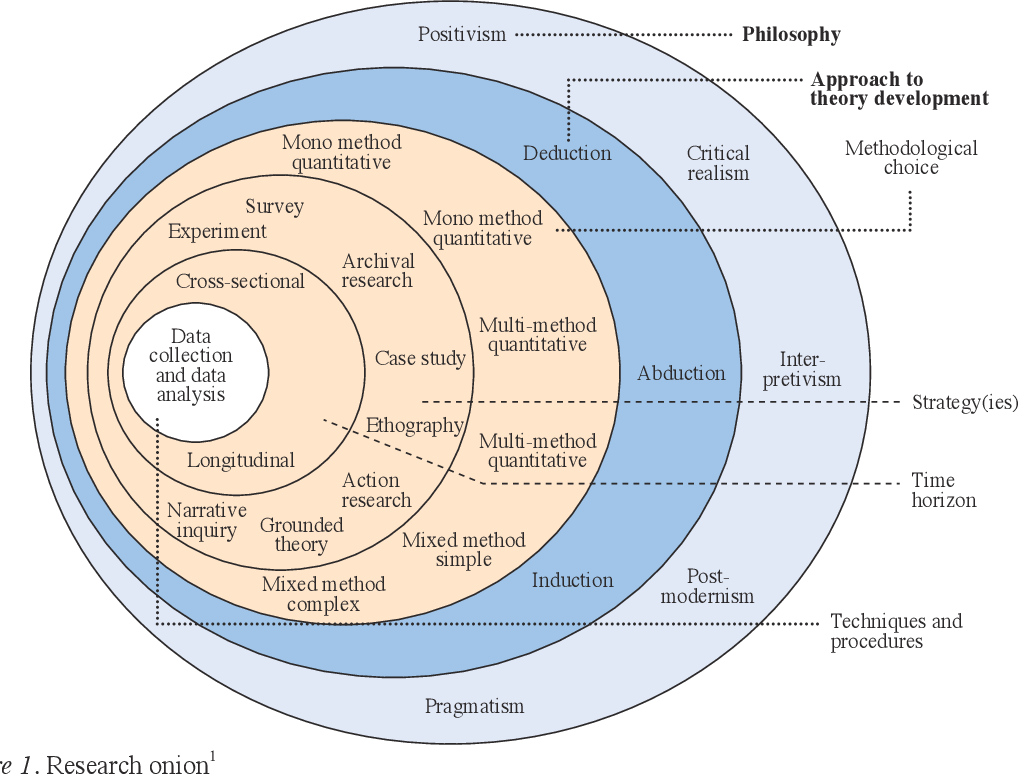
\includegraphics{images/onion.png}

Source: \href{https://www.researchgate.net/profile/Mark-Saunders-10/publication/330760964_Research_Methods_for_Business_Students_Chapter_4_Understanding_research_philosophy_and_approaches_to_theory_development/links/5c53056f299bf12be3f0e2cf/Research-Methods-for-Business-Students-Chapter-4-Understanding-research-philosophy-and-approaches-to-theory-development.pdf}{Saunders, Lewis and Thornhill (2019), Research methods for
business
students}

\hypertarget{alternative-platforms-for-writing-projects}{%
\chapter{Alternative platforms for writing projects}\label{alternative-platforms-for-writing-projects}}

This is a brief list of options when writing a project. Some options are best suited to complex data work, such as Rmarkdown, whereas others are better suited to collaborative writing, such as Overleaf, MS Word via MS Teams.

Each of these platforms are presented in short videos below. There are some clear advantages to using some rather than others. For each you will need to have some knowledge about how the program works in order to use it, and this might require a time investment.

My preference is to recommend open-source options that allow for efficient collaboration and / or reproducible research.

\textbf{Free / open source options}

\begin{enumerate}
\def\labelenumi{\arabic{enumi}.}
\item
  Overleaf / LaTeX
\item
  RMarkdown
\item
  Google Docs (but you pay in terms of data security)
\end{enumerate}

\textbf{Paid / Subscription options}

\begin{enumerate}
\def\labelenumi{\arabic{enumi}.}
\tightlist
\item
  MS Word
\end{enumerate}

\hypertarget{overleaf-latex}{%
\section{Overleaf (LaTeX)}\label{overleaf-latex}}

Overleaf offers a number of excellent guides for getting started, but for those that would like an explanation from me of some of the basics, please feel free to watch the following videos.

One of the most powerful features of Overleaf is the ability to who any change is attributed to, and to roll back changes incrementally. This is possible due to the built in version control features that the platform offers.

\begin{enumerate}
\def\labelenumi{\arabic{enumi}.}
\item
  \href{https://www.youtube.com/watch?v=g8Ejj0T0yG4}{Video: How open an account in Overleaf}
\item
  \href{https://github.com/robabsmith/Example-project}{GitHub: Template documents and resources}
\item
  \href{https://www.loom.com/share/6d0d4f7108f041d082253c636a52dee8}{Video: Integration of Mendely with Overleaf}
\item
  \href{https://youtu.be/BAt5xYP70u0}{Integration of Git with Overleaf (Quite a heavy Spanish accent, but a good guide)}
\end{enumerate}

\hypertarget{rmarkdown}{%
\section{RMarkdown}\label{rmarkdown}}

RMarkdown is a derivative of Markdown syntax, and is a very simple way to write. The video guide below covers a lot of ground, and uses the GitHub template that follows as an example.

\begin{enumerate}
\def\labelenumi{\arabic{enumi}.}
\item
  \href{https://www.loom.com/share/407ae8d0f00e4a05941a9a09e5e13f96}{Video: Getting started with Rmarkdown}
\item
  \href{https://github.com/robabsmith/Rmarkdown-project-template}{GitHub: Project template for single or multi-file projects}
\end{enumerate}

\hypertarget{ms-word-via-ms-teams}{%
\section{MS Word via MS Teams}\label{ms-word-via-ms-teams}}

MS Word files can be dropped into the ``General'' chat area of any Team created using the MS Teams app. These files can then be edited simultaneously by all team members.

\hypertarget{reference-and-bibliography-management}{%
\chapter{Reference and bibliography management}\label{reference-and-bibliography-management}}

With the aid of technology, it is not possible to very easily and efficiently manage and utilise the literature sources that you need when writing an academic project.

The first step is finding the appropriate literature, which is explained in more detail in the chapter below. This section is included in advance as it is useful to select the bibliography management software in advance of completing a literature search.

Each of the more popular reference management software tools have a variety of advantages and disadvantages, depending on what program you choose to work in.

My own preferences are shaped by my experience with each program - and a desire to make sure that the content I create will be accessible to me always, regardless of whether I am at the university or not. If better options exist I would be most interested in hearing about them.

The first two software options enable in-text referencing and automatic generation of reference lists in MS word. The last option, of manually collecting your reference data, is the most inefficient, but has some benefits. The videos below will link to the \href{https://www.loom.com}{Loom} hosting service, and provide a guide to Mendely. Refworks can do pretty much everything that Mendeley can, but it is expensive to use once you leave the university.

\textbf{\textbf{Order of preference}}

\begin{enumerate}
\def\labelenumi{\arabic{enumi}.}
\item
  \href{https://www.mendeley.com/download-desktop-new/}{Mendeley}
\item
  \href{https://www.aub.aau.dk/software-web/refworks/}{Refworks}
\item
  \href{https://youtu.be/JwXQb25cpqA}{Manual storage}
\end{enumerate}

\hypertarget{videos-of-reference-software}{%
\section{Videos of reference software}\label{videos-of-reference-software}}

\begin{enumerate}
\def\labelenumi{\arabic{enumi}.}
\item
  \href{https://youtu.be/MiKbS01Aulo}{Video: Mendeley in 5 minutes: Part 1}
  \href{https://youtu.be/kSu4tO8Dwak}{Video: Mendeley in 5 minutes: Part 2}
  \href{https://youtu.be/XU3cjfY4G5s}{Video: Mendeley in 5 minutes: Part 3}
\item
  \href{https://youtu.be/XTfVCiksapk}{Use of in-text referencing in Ms Word}
\item
  \href{https://youtu.be/zkrVbBSrK_w}{In-text referencing, and creating a reference list in Ms Word}
\item
  \href{https://www.loom.com/share/6d0d4f7108f041d082253c636a52dee8}{Integration of Mendely and Overleaf}
\item
  \href{https://github.com/robabsmith/Example-project}{GitHub Example: Citation options and text edit options in Overleaf}
\item
  \href{https://www.loom.com/share/407ae8d0f00e4a05941a9a09e5e13f96}{Video: Reference lists in RMarkdown}
\item
  \href{https://www.loom.com/share/407ae8d0f00e4a05941a9a09e5e13f96}{Video: Citation options in RMarkdown (Same video as in 6. above)}
\end{enumerate}

\hypertarget{literature-searching}{%
\chapter{Literature searching}\label{literature-searching}}

Literature searches can be completed in a number of ways. There are several very useful free literature search options, as well as more expensive options that you will have access to as a university student.

\hypertarget{free-search-options}{%
\section{Free search options}\label{free-search-options}}

\begin{enumerate}
\def\labelenumi{\arabic{enumi}.}
\tightlist
\item
  \href{https://scholar.google.com}{Google Scholar}
\item
  \href{https://www.semanticscholar.org}{Semantic Scholar}
\end{enumerate}

\hypertarget{paid-search-options}{%
\section{Paid search options}\label{paid-search-options}}

These options are very effectively combined and the University library website. Where the \emph{Primo} service can be used to search a wide variety of databases for a specific search string (or phrase).

\begin{enumerate}
\def\labelenumi{\arabic{enumi}.}
\tightlist
\item
  \href{https://www.en.aub.aau.dk}{Aalborg University Universitetsbiblioteket}
\end{enumerate}

The university site also allows students to access each of the available underlying databases individually and use the special search features that are available for each. Several of these databases allow for bulk exportation of bibliographic information, and can be easily synchronised with referencing software described in the section above.

\begin{enumerate}
\def\labelenumi{\arabic{enumi}.}
\setcounter{enumi}{1}
\tightlist
\item
  \href{https://www.en.aub.aau.dk/find-material/databases}{Databases and suppliers}
\end{enumerate}

A short video introdution to literature search is included as a video reference below. This link will take you to a video recorded and stored on the \textbf{Loom} hosting platform.

\hypertarget{literature-search-videos}{%
\section{Literature search videos}\label{literature-search-videos}}

\begin{enumerate}
\def\labelenumi{\arabic{enumi}.}
\item
  \href{}{How to conduct an efficient literature search}
\item
  \href{}{How to construct the key search criteria for your literature search}
\item
  \href{}{How to save and export search results}
\end{enumerate}

\hypertarget{appendix-literature-search-construction}{%
\chapter{Appendix: Literature search construction}\label{appendix-literature-search-construction}}

\hypertarget{project-title}{%
\section{Project title}\label{project-title}}

Stock-flow consistent models -- property and mortgage

\hypertarget{description-of-subject}{%
\section{Description of subject}\label{description-of-subject}}

Stock flow consistent model to cover mortgage debt of the household sector

\hypertarget{problem-statement-for-project}{%
\section{Problem statement for project}\label{problem-statement-for-project}}

Debt to disposable income levels in several Danish sectors have risen to the highest ever recorded levels, while the Danish central bank (Danmarks nationalbank), the IMF and Finanstilsynet all report that there are no serious threats to financial stability. Financial deregulation, relaxation of borrowing criteria and product innovation have been cited as the leading causes of this trend. This thesis aims to explore credit creation and macro-financial risks related to the expansion of household debt in Denmark by examining institutional sector and individual household balance sheets.

\hypertarget{search-criteria-development-summary}{%
\section{Search criteria development -- summary}\label{search-criteria-development-summary}}

\begin{enumerate}
\def\labelenumi{\arabic{enumi}.}
\tightlist
\item
  Step 01: List all concepts
\item
  Step 02: Group words into ``Blocks'' of concepts
\item
  Step 03: Check for any synonyms
\item
  Step 04: Add Boolean operators
\item
  Step 05: Prioritise blocks according to subject
\item
  Step 06: Selection of appropriate databases
\item
  Step 07: Perform search block by block
\item
  Step 08: Combine search blocks
\item
  Step 09: Refine search parameters based on results
\item
  Step 10: Document search results and search limiters
\item
  Step 11: Compare results and refine search parameters
\item
  Step 12: Export final list of documents
\item
  Step 13: Repeat steps 07 to 12 for each database
\item
  Step 14: Remove duplicates identified from different databases
\item
  Step 15: Remove non-relevant documents based on title and abstract
\item
  Step 16: Read core literature
\item
  Step 17: From core reading, find and read any key literature identified by other authors.
\end{enumerate}

\hypertarget{search-criteria-development}{%
\section{Search criteria development}\label{search-criteria-development}}

\hypertarget{step-01-list-all-concepts}{%
\subsection{Step 01: List all concepts}\label{step-01-list-all-concepts}}

\begin{enumerate}
\def\labelenumi{\arabic{enumi}.}
\tightlist
\item
  Stock Flow Consistent Models
\item
  Structural Econometric Models
\item
  Mortgage debt
\item
  Housing market
\item
  Macroeconomic models
\item
  Post Keynesian theory
\item
  Denmark
\item
  Households
\item
  Sector balance analysis
\item
  Household debt
\end{enumerate}

\hypertarget{step-02-group-words-into-blocks-of-concepts}{%
\subsection{Step 02: Group words into ``Blocks'' of concepts}\label{step-02-group-words-into-blocks-of-concepts}}

\begin{enumerate}
\def\labelenumi{\arabic{enumi}.}
\tightlist
\item
  ``Stock Flow Consistent Models'' OR ``Structural Econometric Models'' OR ``Sector balance analysis''
\item
  ``Macroeconomic''
\item
  ``Mortgage debt'' OR ``Housing market''
\item
  ``Post Keynesian theory''
\item
  ``Denmark''
\item
  ``Households''
\item
  ``debt'' OR Credit''
\end{enumerate}

\hypertarget{step-03-check-for-any-synonyms-and-use-ms-word-to-check-for-spelling-errors}{%
\subsection{Step 03: Check for any synonyms (and use MS Word to check for spelling errors)}\label{step-03-check-for-any-synonyms-and-use-ms-word-to-check-for-spelling-errors}}

\begin{enumerate}
\def\labelenumi{\arabic{enumi}.}
\tightlist
\item
  ``Stock Flow Consistent Models'' OR ``stock flow consistent'' OR ``Stock-flow consistent'' OR ``SFC models'' OR ``SFC'' OR ``Structural Econometric Models'' OR ``Structural econometric'' OR ``SEM models'' OR ``Sector balance analysis'' OR ``SBA'' OR ``Sector financial balances''
\item
  ``Macroeconomic model'' OR ``National model'' OR ``aggregate model''
\item
  ``Mortgage debt'' OR ``mortgage bonds'' OR ``Mortgage credit'' OR ``mortgage borrowing'' OR ``Housing market''
\item
  ``Post Keynesian'' OR ``Post-keynesian''
\item
  ``Denmark'' OR ``Danish'' OR ``Nordic'' OR ``Scandinavian''
\item
  ``Households''
\item
  ``debt'' OR Credit''
\end{enumerate}

\hypertarget{step-04-add-boolean-operators}{%
\subsection{Step 04: Add Boolean operators}\label{step-04-add-boolean-operators}}

\begin{enumerate}
\def\labelenumi{\arabic{enumi}.}
\tightlist
\item
  ``Stock Flow Consistent Model*'' OR ``stock flow consistent'' OR ``Stock-flow consistent'' OR ``SFC model*'' OR ``SFC'' OR ``Structural Econometric Model*'' OR ``Structural econometric'' OR ``SEM model*'' OR ``Sector* balance analysis'' OR ``SBA'' OR ``Sector* financial balance*''
\item
  ``Macroeconomic model*'' OR ``National model*'' OR ``aggregate model*''
\item
  ``Mortgage debt'' OR ``mortgage bonds'' OR ``Mortgage credit'' OR ``mortgage borrowing'' OR ``Housing debt''
\item
  ``Post Keynesian'' OR ``Post-Keynesian''
\item
  ``Denmark'' OR ``Danish'' OR ``Nordic'' OR ``Scandinavian''
\item
  ``Household*''
\item
  ``debt'' OR Credit''
\end{enumerate}

\hypertarget{step-05-prioritise-blocks-according-to-subject}{%
\subsection{Step 05: Prioritise blocks according to subject}\label{step-05-prioritise-blocks-according-to-subject}}

\textbf{Starting with the most relevant first}

(``Stock Flow Consistent'' OR ``Stock-flow consistent'' OR ``SFC model*'')

OR

(``Structural Econometric'' OR ``SEM model*'')

AND

(``Macroeconomic model*'' OR ``National model*'' OR ``aggregate model*'' OR ``sector* model'')

AND

(``Mortgage debt'' OR ``mortgage bonds'' OR ``Mortgage credit'' OR ``mortgage borrowing'' OR ``Housing debt'' OR ``Housing market'' OR ``Property market'' OR ``Property Prices'')

AND

(``Post Keynesian'' OR ``Post-Keynesian'')

AND

(``Denmark*'' OR ``Danish'' OR ``Nordic'' OR ``Scandinavia*'')

AND

(``Household*'' OR ``private sector'')

AND

(``debt'' OR ``Credit'')

\textbf{Optional alternative to add to SFC}
(``Sector* balance analys*'' OR ``Sector* financial balance*'')

\hypertarget{step-06-perform-search-block-by-block}{%
\subsection{Step 06: Perform search block by block}\label{step-06-perform-search-block-by-block}}

\hypertarget{step-07-combine-search-blocks}{%
\subsection{Step 07: Combine search blocks}\label{step-07-combine-search-blocks}}

\hypertarget{step-08-document-search-results-and-limitations}{%
\subsection{Step 08: Document search results and limitations}\label{step-08-document-search-results-and-limitations}}

\hypertarget{step-09-compare-results-and-refine-search-parameters}{%
\subsection{Step 09: Compare results and refine search parameters}\label{step-09-compare-results-and-refine-search-parameters}}

\hypertarget{scopus}{%
\subsubsection{1. Scopus}\label{scopus}}

\textbf{Scopus (371 results)}

\emph{Search string:}

ALL((``Stock Flow Consistent'' OR ``Stock-Flow Consistent'') AND (macroeconomic* model*)) AND DOCTYPE(ar OR re OR bk OR ch OR cp OR sh) AND (LIMIT-TO(LANGUAGE, ``English''))

\textbf{Scopus (138 results)}

\emph{Search string:}

TITLE (``Stock Flow Consistent'' OR ``Stock-Flow Consistent'' OR ``SFC'') AND ALL ( ``propert*'' OR ``hous*'' OR ``mortgage'') AND DOCTYPE ( ar OR re OR bk OR ch OR cp OR sh ) AND ( LIMIT-TO ( LANGUAGE , ``English'' ) )

\textbf{Scopus (6 results) + housing}

\emph{Search string:}

TITLE (``Stock Flow Consistent'' OR ``Stock-Flow Consistent'' OR ``SFC'') AND ALL (``housing'') AND DOCTYPE ( ar OR re OR bk OR ch OR cp OR sh ) AND ( LIMIT-TO ( LANGUAGE , ``English'' ) )

\textbf{Scopus (3 results) + mortgage}

\emph{Search string:}

TITLE ( ``Stock Flow Consistent'' OR ``Stock-Flow Consistent'' OR ``SFC'') AND ALL (``mortgage'') AND DOCTYPE ( ar OR re OR bk OR ch OR cp OR sh ) AND ( LIMIT-TO ( LANGUAGE , ``English'' ) )

\textbf{Scopus (26 results) + property housing mortgage}

\emph{Search string:}

TITLE ( ``Stock Flow Consistent'' OR ``Stock-Flow Consistent'' OR ``SFC'' ) AND ALL ( ``propert*'' OR ``hous*'' OR ``mortgage'' ) AND DOCTYPE ( ar OR re OR bk OR ch OR cp OR sh ) AND NOT ( ``Chromatography'' OR ``lipid solid fat'' OR ``solid fat content'' OR ``silico-ferrite off calcium'' OR molecular* OR ``service function chaining'' OR ``service-function chaining'' OR ``chemistry'' OR ``space-filling curve'' OR ``Sequential Function Chart*'' OR ``SFC binder'' ) AND ( LIMIT-TO ( LANGUAGE , ``English'' ) )

\textbf{Scopus (23 results) + property housing mortgage}

\emph{Search string:}

TITLE ( ``Stock Flow Consistent'' OR ``Stock-Flow Consistent'' OR ``SFC'' ) AND ALL ( ``property market'' OR ``housing market'' OR ``mortgage debt'' ) AND ALL ( ``economics'' ) AND DOCTYPE ( ar OR re OR bk OR ch OR cp OR sh ) AND ( LIMIT-TO ( LANGUAGE , ``English'' ) )

\hypertarget{ebscohost-business-source-premier-academic-source-premier-119-results}{%
\subsubsection{2. EBSCOhost (Business Source Premier, Academic Source Premier) (119 results)}\label{ebscohost-business-source-premier-academic-source-premier-119-results}}

(Search options: Also search in full text of the articles)

(Limits: Academic search premier
Language: English
Publication Type: All
Document Type: Article, book chapter, proceeding, report)

(Limits: Business search premier
Language: English
Publication Type: Academic journal, Book
Document Type: Article, book entry, proceeding, report, working paper)

\textbf{EBSCOhost (119 results)}

\emph{Search string:}

(``Stock Flow Consistent'' OR ``Stock-Flow Consistent'')
AND
(macroeconomic* model*)

\textbf{EBSCOhost (25 results) (included)}

\emph{Search string:}

(``Stock Flow Consistent'' OR ``Stock-Flow Consistent'' OR ``SFC'') (Limit: TITLE)
AND
(macroeconomic* model*)

\textbf{EBSCOhost (9 results)}

\emph{Search string:}

(``Stock Flow Consistent'' OR ``Stock-Flow Consistent'')
AND
(macroeconomic* model*)
AND
(``Denmark*'' OR ``Danish'' OR ``Nordic'' OR ``Scandinavia*'')

\hypertarget{proquest}{%
\subsubsection{3. ProQuest}\label{proquest}}

\textbf{ProQuest (529 results)}

\emph{Search string:}

(``Stock Flow Consistent'' OR ``Stock-Flow Consistent'' OR ``SFC'') AND (macroeconomic* AND model*) AND (LA(English))

\textbf{ProQuest (43 results)}

\emph{Search string:}

TI(``Stock Flow Consistent'' OR ``Stock-Flow Consistent'' OR ``SFC'' ) AND ALL (macroeconomic* AND model*) AND (LA(English))

\textbf{Source type}

Conference Papers \& Proceedings, Dissertations \& Theses, Scholarly Journals, Working Papers

\textbf{Document type}

Article, Book, Book Chapter, Conference Paper, Country Report, Literature Review, Report, Technical Report, Working Paper/Pre-Print

\textbf{Language}

English

\hypertarget{jstor}{%
\subsubsection{4. JSTOR}\label{jstor}}

\textbf{JSTOR (96 results) (selection included -- JSTOR requires click to export)}

\emph{Search string:}

((``Stock Flow Consistent'' OR ``Stock-Flow Consistent'') AND (macroeconomic* model*)) AND la:(eng OR en)

\textbf{JSTOR (19 results)}

\emph{Search string:}

(ti:(``Stock Flow Consistent'' OR ``Stock-Flow Consistent'' OR ``SFC'') la:(eng OR en)

\textbf{JSTOR (13 results)}

\emph{Search string:}

(ti:(``Stock Flow Consistent'' OR ``Stock-Flow Consistent'' OR ``SFC'') AND (macroeconomic* model*)) AND la:(eng OR en)

\hypertarget{web-of-science}{%
\subsubsection{5. Web of Science}\label{web-of-science}}

\textbf{Web of Science (67 results)}

\emph{Search string:}

(``Stock Flow Consistent'' OR ``Stock-Flow Consistent'')
AND
(macroeconomic* model*)

\textbf{Web of Science (24 results)}

\emph{Search string:}

(``Stock Flow Consistent'' OR ``Stock-Flow Consistent'' OR ``SFC'') (Limit: TITLE)
AND
(macroeconomic* model*)

\textbf{Web of Science (1 results)}

\emph{Search string:}

(``Stock Flow Consistent'' OR ``Stock-Flow Consistent'')
AND
(macroeconomic* model*)
AND
(``Denmark*'' OR ``Danish'' OR ``Nordic'' OR ``Scandinavia*'')

\hypertarget{summary}{%
\section{Summary}\label{summary}}

Total of 146 documents found

\hypertarget{data-retrieval-and-plotting}{%
\chapter{Data retrieval and plotting}\label{data-retrieval-and-plotting}}

The examples used in this section (excluding the plotly interactive plots at the bottom) can all be found in a complete RMarkdown file called ``SingleDocument.Rmd'' in \href{https://github.com/robabsmith/Rmarkdown-project-template}{one of my other GitHub repositories, here.}

\hypertarget{example-data-sourcing-and-manipulation}{%
\section{Example data sourcing and manipulation}\label{example-data-sourcing-and-manipulation}}

One of the benefits of online database API access is that you can readily source up to date data directly from web locations without having to save files locally in advance.

Most of the major data providers have easy to handle R packages for directly importing data while building your document. The following code chunk requires several packages to be installed:

\hypertarget{loading-the-required-packages}{%
\subsection{Loading the required packages}\label{loading-the-required-packages}}

The first \texttt{sapply} function is just a nice abbreviation that can be used to run the \texttt{require}command for all of the packages listed in the preceding vector. It can of course be modified to run any function.

The second part is particularly useful when writing PDF documents, as you can set the standard chunk options up front in your document and adjust all image settings at once if you choose to change your document setup.

These packages are mostly used in setting up additional plot options for ggplot 2 for aesthetic purposes, like controlling the colour palette, the location and size of the legend etc. All of that plotting code is included just before the plots below.

\hypertarget{collecting-the-data-from-the-danmarks-statistik-api}{%
\subsection{Collecting the data from the Danmarks Statistik API}\label{collecting-the-data-from-the-danmarks-statistik-api}}

\begin{Shaded}
\begin{Highlighting}[]
\DocumentationTok{\#\#\#\#\#\#\#\#\#\#\#\#\#\#\#\#\#\#\#\#\#\#\#\#\#\#\#\#\#\#\#\#\#\#\#\#\#\#\#\#\#\#\#\#\#\#\#\#\#\#\#\#\#\#\#\#\#\#\#\#\#\#\#\#\#\#\#\#\#\#\#\#\#}
\CommentTok{\# Danmarks statistik example}
\DocumentationTok{\#\#\#\#\#\#\#\#\#\#\#\#\#\#\#\#\#\#\#\#\#\#\#\#\#\#\#\#\#\#\#\#\#\#\#\#\#\#\#\#\#\#\#\#\#\#\#\#\#\#\#\#\#\#\#\#\#\#\#\#\#\#\#\#\#\#\#\#\#\#\#\#\#}

\CommentTok{\# This uses a package called statsDK, which needs to be built from Mikkel Krogsholm\textquotesingle{}s the GitHub repo.}
\CommentTok{\# }
\CommentTok{\#    install.packages("devtools")}
\CommentTok{\#    library(devtools)}
\CommentTok{\#    devtools::install\_github("mikkelkrogsholm/statsDK")}

\CommentTok{\# Fetching interest rate data, and filter for mortgage products}
\DocumentationTok{\#\#\#\#\#\#\#\#\#\#\#\#\#\#\#\#\#\#\#\#\#\#\#\#\#\#\#\#\#\#\#\#\#\#\#\#\#\#\#\#\#\#\#\#\#\#\#\#\#\#\#\#\#\#\#\#\#\#\#\#\#\#\#\#\#\#\#\#\#\#\#\#\#}
\NormalTok{dk\_mortgage\_interest\_raw\_data }\OtherTok{\textless{}{-}} \FunctionTok{data.table}\NormalTok{(}\FunctionTok{sdk\_retrieve\_data}\NormalTok{(}\AttributeTok{table\_id =} \StringTok{"DNRNURI"}\NormalTok{, }
                                                              \AttributeTok{DATA =} \FunctionTok{paste0}\NormalTok{(}\FunctionTok{c}\NormalTok{(}\StringTok{"AL51EFFR"}\NormalTok{, }\StringTok{"AL51BIDS"}\NormalTok{),}\AttributeTok{collapse =} \StringTok{","}\NormalTok{),}
                                                              \AttributeTok{INDSEK =} \FunctionTok{paste0}\NormalTok{(}\FunctionTok{c}\NormalTok{(}\StringTok{"1400"}\NormalTok{),}\AttributeTok{collapse =} \StringTok{","}\NormalTok{),}
                                                              \AttributeTok{VALUTA =} \StringTok{"z01"}\NormalTok{, }
\NormalTok{                                                              LØBETID1 }\OtherTok{=} \StringTok{"ALLE"}\NormalTok{,}
                                                              \AttributeTok{RENTFIX =} \FunctionTok{paste0}\NormalTok{(}\FunctionTok{c}\NormalTok{(}\StringTok{"1A"}\NormalTok{, }\StringTok{"2A"}\NormalTok{, }\StringTok{"3A"}\NormalTok{, }\StringTok{"5A"}\NormalTok{, }\StringTok{"10A"}\NormalTok{, }\StringTok{"S10A"}\NormalTok{),}\AttributeTok{collapse =} \StringTok{","}\NormalTok{),}
                                                              \AttributeTok{LAANSTR =} \StringTok{"ALLE"}\NormalTok{,}
                                                              \AttributeTok{Tid =} \StringTok{"*"}\NormalTok{)) }\SpecialCharTok{\%\textgreater{}\%}
    \FunctionTok{select}\NormalTok{(}\SpecialCharTok{{-}}\FunctionTok{c}\NormalTok{(VALUTA, LØBETID1, LAANSTR, INDSEK)) }\SpecialCharTok{\%\textgreater{}\%}
    \CommentTok{\#mutate(Value = str\_replace\_all(INDHOLD, pattern = "..", "")) \%\textgreater{}\%}
    \FunctionTok{mutate}\NormalTok{(}\AttributeTok{Value =} \FunctionTok{as.double}\NormalTok{(INDHOLD, }\AttributeTok{na.rm =} \ConstantTok{TRUE}\NormalTok{)}\SpecialCharTok{/}\DecValTok{100}\NormalTok{,}
           \AttributeTok{RENTFIX =} \FunctionTok{str\_replace\_all}\NormalTok{(RENTFIX, }\AttributeTok{pattern =} \StringTok{" {-} {-} "}\NormalTok{, }\StringTok{""}\NormalTok{)) }\SpecialCharTok{\%\textgreater{}\%}
    \FunctionTok{mutate}\NormalTok{(}\AttributeTok{RENTFIX =} \FunctionTok{str\_replace\_all}\NormalTok{(RENTFIX, }\AttributeTok{pattern =} \StringTok{" {-} "}\NormalTok{, }\StringTok{""}\NormalTok{)) }\SpecialCharTok{\%\textgreater{}\%}
    \FunctionTok{mutate}\NormalTok{(}\AttributeTok{RENTFIX =} \FunctionTok{str\_replace\_all}\NormalTok{(RENTFIX, }\AttributeTok{pattern =} \StringTok{"{-} "}\NormalTok{, }\StringTok{""}\NormalTok{)) }\SpecialCharTok{\%\textgreater{}\%}
    \FunctionTok{mutate}\NormalTok{(}\AttributeTok{RENTFIX =} \FunctionTok{str\_replace\_all}\NormalTok{(RENTFIX, }\AttributeTok{pattern =} \StringTok{"Over 6 months and up to and including 1 year"}\NormalTok{, }\StringTok{"01 year"}\NormalTok{)) }\SpecialCharTok{\%\textgreater{}\%}
    \FunctionTok{mutate}\NormalTok{(}\AttributeTok{RENTFIX =} \FunctionTok{str\_replace\_all}\NormalTok{(RENTFIX, }\AttributeTok{pattern =} \StringTok{"Over 1 year and up to and including 2 years"}\NormalTok{, }\StringTok{"02 year"}\NormalTok{)) }\SpecialCharTok{\%\textgreater{}\%}
    \FunctionTok{mutate}\NormalTok{(}\AttributeTok{RENTFIX =} \FunctionTok{str\_replace\_all}\NormalTok{(RENTFIX, }\AttributeTok{pattern =} \StringTok{"Over 2 years and up to and including 3 years"}\NormalTok{, }\StringTok{"03 year"}\NormalTok{)) }\SpecialCharTok{\%\textgreater{}\%}
    \FunctionTok{mutate}\NormalTok{(}\AttributeTok{RENTFIX =} \FunctionTok{str\_replace\_all}\NormalTok{(RENTFIX, }\AttributeTok{pattern =} \StringTok{"Over 3 years and up to and including 5 years"}\NormalTok{, }\StringTok{"05 year"}\NormalTok{)) }\SpecialCharTok{\%\textgreater{}\%}
    \FunctionTok{mutate}\NormalTok{(}\AttributeTok{RENTFIX =} \FunctionTok{str\_replace\_all}\NormalTok{(RENTFIX, }\AttributeTok{pattern =} \StringTok{"Over 5 years and up to and including 10 years"}\NormalTok{, }\StringTok{"10 year"}\NormalTok{)) }\SpecialCharTok{\%\textgreater{}\%}
    \FunctionTok{mutate}\NormalTok{(}\AttributeTok{Interest\_Fixation =} \FunctionTok{str\_replace\_all}\NormalTok{(RENTFIX, }\AttributeTok{pattern =} \StringTok{"Over 10 years"}\NormalTok{, }\StringTok{"Fixed"}\NormalTok{)) }\SpecialCharTok{\%\textgreater{}\%}
    \FunctionTok{mutate}\NormalTok{(}\AttributeTok{Date =} \FunctionTok{str\_replace\_all}\NormalTok{(TID, }\AttributeTok{pattern =} \StringTok{"M"}\NormalTok{, }\StringTok{""}\NormalTok{)) }\SpecialCharTok{\%\textgreater{}\%}
    \FunctionTok{mutate}\NormalTok{(}\AttributeTok{Date =} \FunctionTok{paste0}\NormalTok{(Date, }\StringTok{"01"}\NormalTok{)) }\SpecialCharTok{\%\textgreater{}\%}
    \FunctionTok{mutate}\NormalTok{(}\AttributeTok{Date =} \FunctionTok{as.Date}\NormalTok{(Date,}\AttributeTok{format=}\StringTok{\textquotesingle{}\%Y\%m\%d\textquotesingle{}}\NormalTok{))  }\SpecialCharTok{\%\textgreater{}\%}
    \FunctionTok{mutate}\NormalTok{(}\AttributeTok{Interest\_Fixation =} \FunctionTok{factor}\NormalTok{(Interest\_Fixation, }\AttributeTok{order =} \ConstantTok{TRUE}\NormalTok{, }
                                      \AttributeTok{levels =} \FunctionTok{c}\NormalTok{(}\StringTok{"01 year"}\NormalTok{,}
                                                 \StringTok{"02 year"}\NormalTok{,}
                                                 \StringTok{"03 year"}\NormalTok{, }
                                                 \StringTok{"05 year"}\NormalTok{,}
                                                 \StringTok{"10 year"}\NormalTok{,}
                                                 \StringTok{"Fixed"}\NormalTok{))) }\SpecialCharTok{\%\textgreater{}\%}
    \FunctionTok{select}\NormalTok{(}\SpecialCharTok{{-}}\NormalTok{INDHOLD, }\SpecialCharTok{{-}}\NormalTok{RENTFIX, }\SpecialCharTok{{-}}\NormalTok{TID) }\SpecialCharTok{\%\textgreater{}\%}
    \FunctionTok{filter}\NormalTok{(}\SpecialCharTok{!}\FunctionTok{is.na}\NormalTok{(Value))}


\NormalTok{DK\_yield\_curves\_rates }\OtherTok{\textless{}{-}}\NormalTok{ dk\_mortgage\_interest\_raw\_data }\SpecialCharTok{\%\textgreater{}\%}
    \FunctionTok{filter}\NormalTok{(DATA }\SpecialCharTok{!=} \StringTok{"Administration rate (per cent) (not indexed)"}\NormalTok{,}
           \SpecialCharTok{!}\FunctionTok{is.na}\NormalTok{(Value)) }\SpecialCharTok{\%\textgreater{}\%}
    \FunctionTok{select}\NormalTok{(}\SpecialCharTok{{-}}\NormalTok{DATA)}
\end{Highlighting}
\end{Shaded}

\hypertarget{adding-some-extra-plotting-options}{%
\subsection{Adding some extra plotting options}\label{adding-some-extra-plotting-options}}

This section includes some additional code that makes writing a document a little more user friendly.

The first part includes some directory specifications, based on the
location that the user saves this file.

The second part includes a number of ggplot2 theme and colour palette
modifications that can be modified for personal preference.

\begin{itemize}
\tightlist
\item
  The line-width for all line plots in the document.
\item
  Palettes with shades of red, black, blue for 4 5 and 6 variables.
\item
  A mixed colour palette of 10 colours for categorical variables.
\item
  Alternative legend placements inside the plotting area.
  (This saves a lot of space in the final document).
\item
  Percentage formats that work with latex and ggplot2.
\item
  Simplified command to introduce dashed lines for 5 and 6 variables.
\item
  A theme adjustment to reduce font size in all plots.
\end{itemize}

\begin{Shaded}
\begin{Highlighting}[]
\DocumentationTok{\#\#\#\#\#\#\#\#\#\#\#\#\#\#\#\#\#\#\#\#\#\#\#\#\#\#\#\#\#\#\#\#\#\#\#\#\#\#\#\#\#\#\#\#\#\#\#\#\#\#\#\#\#\#\#\#\#\#\#\#\#\#\#\#\#\#\#\#\#\#\#\#\#}
\CommentTok{\# Set up some extra features for plots that will be used later}

\NormalTok{plot\_line\_width }\OtherTok{=} \FloatTok{0.85}

\DocumentationTok{\#\#\#\#\#\#\#\#\#\#\#\#\#\#\#\#\#\#\#\#\#\#\#\#\#\#\#\#\#\#\#\#\#\#\#\#\#\#\#\#\#\#\#\#\#\#\#\#\#\#\#\#\#\#\#\#\#\#\#\#\#\#\#\#\#\#\#\#\#\#\#\#\#}
\CommentTok{\# Set colour palettes}
\DocumentationTok{\#\#\#\#\#\#\#\#\#\#\#\#\#\#\#\#\#\#\#\#\#\#\#\#\#\#\#\#\#\#\#\#\#\#\#\#\#\#\#\#\#\#\#\#\#\#\#\#\#\#\#\#\#\#\#\#\#\#\#\#\#\#\#\#\#\#\#\#\#\#\#\#\#}

\NormalTok{blackpalette }\OtherTok{\textless{}{-}} \FunctionTok{c}\NormalTok{(}\StringTok{"0, 0, 0"}\NormalTok{,}
                  \StringTok{"125, 125, 125"}\NormalTok{,}
                  \StringTok{"75, 75, 75"}\NormalTok{,}
                  \StringTok{"225, 30, 0"}\NormalTok{)}
\NormalTok{bluepalette }\OtherTok{\textless{}{-}} \FunctionTok{c}\NormalTok{(}\StringTok{"0, 50, 130"}\NormalTok{,}
                 \StringTok{"0, 170, 255"}\NormalTok{,}
                 \StringTok{"0, 200, 255"}\NormalTok{,}
                 \StringTok{"0, 55, 255"}\NormalTok{)}
\NormalTok{redpalette }\OtherTok{\textless{}{-}} \FunctionTok{c}\NormalTok{(}\StringTok{"255, 45, 0"}\NormalTok{,}
                \StringTok{"255, 200, 0"}\NormalTok{,}
                \StringTok{"255, 155, 0"}\NormalTok{,}
                \StringTok{"255, 100, 0"}\NormalTok{)}

\NormalTok{blackpalette\_five }\OtherTok{\textless{}{-}} \FunctionTok{c}\NormalTok{(}\StringTok{"0, 0, 0"}\NormalTok{,}
                       \StringTok{"185, 190, 200"}\NormalTok{,}
                       \StringTok{"115, 115, 115"}\NormalTok{,}
                       \StringTok{"75, 75, 75"}\NormalTok{,}
                       \StringTok{"225, 30, 0"}\NormalTok{)}
\NormalTok{bluepalette\_five }\OtherTok{\textless{}{-}} \FunctionTok{c}\NormalTok{(}\StringTok{"0, 50, 130"}\NormalTok{,}
                      \StringTok{"0, 150, 255"}\NormalTok{,}
                      \StringTok{"0, 175, 255"}\NormalTok{,}
                      \StringTok{"0, 200, 255"}\NormalTok{,}
                      \StringTok{"0, 55, 255"}\NormalTok{)}
\NormalTok{redpalette\_five }\OtherTok{\textless{}{-}} \FunctionTok{c}\NormalTok{(}\StringTok{"255, 45, 0"}\NormalTok{,}
                     \StringTok{"255, 200, 0"}\NormalTok{,}
                     \StringTok{"255, 175, 0"}\NormalTok{,}
                     \StringTok{"255, 145, 0"}\NormalTok{,}
                     \StringTok{"255, 100, 0"}\NormalTok{)}

\NormalTok{blackpalette\_six }\OtherTok{\textless{}{-}} \FunctionTok{c}\NormalTok{(}\StringTok{"0, 50, 130"}\NormalTok{,}
                      \StringTok{"0, 0, 0"}\NormalTok{,}
                      \StringTok{"185, 190, 200"}\NormalTok{,}
                      \StringTok{"115, 115, 115"}\NormalTok{,}
                      \StringTok{"75, 75, 75"}\NormalTok{,}
                      \StringTok{"225, 30, 0"}\NormalTok{)}
\NormalTok{bluepalette\_six }\OtherTok{\textless{}{-}} \FunctionTok{c}\NormalTok{(}\StringTok{"0, 50, 130"}\NormalTok{,}
                     \StringTok{"0, 100, 255"}\NormalTok{,}
                     \StringTok{"0, 130, 255"}\NormalTok{,}
                     \StringTok{"0, 165, 255"}\NormalTok{,}
                     \StringTok{"0, 200, 255"}\NormalTok{,}
                     \StringTok{"0, 55, 255"}\NormalTok{)}
\NormalTok{redpalette\_six }\OtherTok{\textless{}{-}} \FunctionTok{c}\NormalTok{(}\StringTok{"255, 45, 0"}\NormalTok{,}
                    \StringTok{"255, 240, 0"}\NormalTok{,}
                    \StringTok{"255, 210, 0"}\NormalTok{,}
                    \StringTok{"255, 180, 0"}\NormalTok{,}
                    \StringTok{"255, 155, 0"}\NormalTok{,}
                    \StringTok{"255, 100, 0"}\NormalTok{)}

\NormalTok{randompalette }\OtherTok{\textless{}{-}} \FunctionTok{c}\NormalTok{(}\StringTok{"91, 163, 111"}\NormalTok{,}
                   \StringTok{"84, 135, 158"}\NormalTok{,}
                   \StringTok{"76, 99, 143"}\NormalTok{,}
                   \StringTok{"204, 157, 2"}\NormalTok{,}
                   \StringTok{"156, 0, 0"}\NormalTok{,}
                   \StringTok{"110, 99, 194"}\NormalTok{,}
                   \StringTok{"11, 132, 176"}\NormalTok{,}
                   \StringTok{"237, 133, 28"}\NormalTok{,}
                   \StringTok{"23, 87, 11"}\NormalTok{,}
                   \StringTok{"49, 163, 79"}\NormalTok{)}

\NormalTok{blackpalette }\OtherTok{\textless{}{-}} \FunctionTok{sapply}\NormalTok{(}\FunctionTok{strsplit}\NormalTok{(blackpalette, }\StringTok{", "}\NormalTok{), }\ControlFlowTok{function}\NormalTok{(x)}
    \FunctionTok{rgb}\NormalTok{(x[}\DecValTok{1}\NormalTok{], x[}\DecValTok{2}\NormalTok{], x[}\DecValTok{3}\NormalTok{], }\AttributeTok{maxColorValue=}\DecValTok{255}\NormalTok{))}
\NormalTok{bluepalette }\OtherTok{\textless{}{-}} \FunctionTok{sapply}\NormalTok{(}\FunctionTok{strsplit}\NormalTok{(bluepalette, }\StringTok{", "}\NormalTok{), }\ControlFlowTok{function}\NormalTok{(x)}
    \FunctionTok{rgb}\NormalTok{(x[}\DecValTok{1}\NormalTok{], x[}\DecValTok{2}\NormalTok{], x[}\DecValTok{3}\NormalTok{], }\AttributeTok{maxColorValue=}\DecValTok{255}\NormalTok{))}
\NormalTok{redpalette }\OtherTok{\textless{}{-}} \FunctionTok{sapply}\NormalTok{(}\FunctionTok{strsplit}\NormalTok{(redpalette, }\StringTok{", "}\NormalTok{), }\ControlFlowTok{function}\NormalTok{(x)}
    \FunctionTok{rgb}\NormalTok{(x[}\DecValTok{1}\NormalTok{], x[}\DecValTok{2}\NormalTok{], x[}\DecValTok{3}\NormalTok{], }\AttributeTok{maxColorValue=}\DecValTok{255}\NormalTok{))}

\NormalTok{blackpalette\_five }\OtherTok{\textless{}{-}} \FunctionTok{sapply}\NormalTok{(}\FunctionTok{strsplit}\NormalTok{(blackpalette\_five, }\StringTok{", "}\NormalTok{), }\ControlFlowTok{function}\NormalTok{(x)}
    \FunctionTok{rgb}\NormalTok{(x[}\DecValTok{1}\NormalTok{], x[}\DecValTok{2}\NormalTok{], x[}\DecValTok{3}\NormalTok{], }\AttributeTok{maxColorValue=}\DecValTok{255}\NormalTok{))}
\NormalTok{bluepalette\_five }\OtherTok{\textless{}{-}} \FunctionTok{sapply}\NormalTok{(}\FunctionTok{strsplit}\NormalTok{(bluepalette\_five, }\StringTok{", "}\NormalTok{), }\ControlFlowTok{function}\NormalTok{(x)}
    \FunctionTok{rgb}\NormalTok{(x[}\DecValTok{1}\NormalTok{], x[}\DecValTok{2}\NormalTok{], x[}\DecValTok{3}\NormalTok{], }\AttributeTok{maxColorValue=}\DecValTok{255}\NormalTok{))}
\NormalTok{redpalette\_five }\OtherTok{\textless{}{-}} \FunctionTok{sapply}\NormalTok{(}\FunctionTok{strsplit}\NormalTok{(redpalette\_five, }\StringTok{", "}\NormalTok{), }\ControlFlowTok{function}\NormalTok{(x)}
    \FunctionTok{rgb}\NormalTok{(x[}\DecValTok{1}\NormalTok{], x[}\DecValTok{2}\NormalTok{], x[}\DecValTok{3}\NormalTok{], }\AttributeTok{maxColorValue=}\DecValTok{255}\NormalTok{))}

\NormalTok{blackpalette\_six }\OtherTok{\textless{}{-}} \FunctionTok{sapply}\NormalTok{(}\FunctionTok{strsplit}\NormalTok{(blackpalette\_six, }\StringTok{", "}\NormalTok{), }\ControlFlowTok{function}\NormalTok{(x)}
    \FunctionTok{rgb}\NormalTok{(x[}\DecValTok{1}\NormalTok{], x[}\DecValTok{2}\NormalTok{], x[}\DecValTok{3}\NormalTok{], }\AttributeTok{maxColorValue=}\DecValTok{255}\NormalTok{))}
\NormalTok{bluepalette\_six }\OtherTok{\textless{}{-}} \FunctionTok{sapply}\NormalTok{(}\FunctionTok{strsplit}\NormalTok{(bluepalette\_six, }\StringTok{", "}\NormalTok{), }\ControlFlowTok{function}\NormalTok{(x)}
    \FunctionTok{rgb}\NormalTok{(x[}\DecValTok{1}\NormalTok{], x[}\DecValTok{2}\NormalTok{], x[}\DecValTok{3}\NormalTok{], }\AttributeTok{maxColorValue=}\DecValTok{255}\NormalTok{))}
\NormalTok{redpalette\_six }\OtherTok{\textless{}{-}} \FunctionTok{sapply}\NormalTok{(}\FunctionTok{strsplit}\NormalTok{(redpalette\_six, }\StringTok{", "}\NormalTok{), }\ControlFlowTok{function}\NormalTok{(x)}
    \FunctionTok{rgb}\NormalTok{(x[}\DecValTok{1}\NormalTok{], x[}\DecValTok{2}\NormalTok{], x[}\DecValTok{3}\NormalTok{], }\AttributeTok{maxColorValue=}\DecValTok{255}\NormalTok{))}

\NormalTok{randompalette }\OtherTok{\textless{}{-}} \FunctionTok{sapply}\NormalTok{(}\FunctionTok{strsplit}\NormalTok{(randompalette, }\StringTok{", "}\NormalTok{), }\ControlFlowTok{function}\NormalTok{(x)}
    \FunctionTok{rgb}\NormalTok{(x[}\DecValTok{1}\NormalTok{], x[}\DecValTok{2}\NormalTok{], x[}\DecValTok{3}\NormalTok{], }\AttributeTok{maxColorValue=}\DecValTok{255}\NormalTok{))}


\DocumentationTok{\#\#\#\#\#\#\#\#\#\#\#\#\#\#\#\#\#\#\#\#\#\#\#\#\#\#\#\#\#\#\#\#\#\#\#\#\#\#\#\#\#\#\#\#\#\#\#\#\#\#\#\#\#\#\#\#\#\#\#\#\#\#\#\#\#\#\#\#\#\#\#\#\#}
\CommentTok{\# Define random colours for plots and theme settings}
\DocumentationTok{\#\#\#\#\#\#\#\#\#\#\#\#\#\#\#\#\#\#\#\#\#\#\#\#\#\#\#\#\#\#\#\#\#\#\#\#\#\#\#\#\#\#\#\#\#\#\#\#\#\#\#\#\#\#\#\#\#\#\#\#\#\#\#\#\#\#\#\#\#\#\#\#\#}

\NormalTok{random\_srv\_palette }\OtherTok{\textless{}{-}} \FunctionTok{c}\NormalTok{(}\StringTok{"91, 163, 111"}\NormalTok{,}
                        \StringTok{"84, 135, 158"}\NormalTok{,}
                        \StringTok{"156, 0, 0"}\NormalTok{,}
                        \StringTok{"204, 157, 2"}\NormalTok{,}
                        \StringTok{"110, 99, 194"}\NormalTok{,}
                        \StringTok{"11, 132, 176"}\NormalTok{,}
                        \StringTok{"76, 99, 143"}\NormalTok{,}
                        \StringTok{"237, 133, 28"}\NormalTok{,}
                        \StringTok{"23, 87, 11"}\NormalTok{,}
                        \StringTok{"11, 132, 176"}\NormalTok{,}
                        \StringTok{"49, 163, 79"}\NormalTok{)}
\NormalTok{random\_srv\_palette }\OtherTok{\textless{}{-}} \FunctionTok{sapply}\NormalTok{(}\FunctionTok{strsplit}\NormalTok{(random\_srv\_palette, }\StringTok{", "}\NormalTok{), }\ControlFlowTok{function}\NormalTok{(x)}
    \FunctionTok{rgb}\NormalTok{(x[}\DecValTok{1}\NormalTok{], x[}\DecValTok{2}\NormalTok{], x[}\DecValTok{3}\NormalTok{], }\AttributeTok{maxColorValue =} \DecValTok{255}\NormalTok{))}

\DocumentationTok{\#\#\#\#\#\#\#\#\#\#\#\#\#\#\#\#\#\#\#\#\#\#\#\#\#\#\#\#\#\#\#\#\#\#\#\#\#\#\#\#\#\#\#\#\#\#\#\#\#\#\#\#\#\#\#\#\#\#\#\#\#\#\#\#\#\#\#\#\#\#\#\#\#}
\CommentTok{\# Set plot options}
\DocumentationTok{\#\#\#\#\#\#\#\#\#\#\#\#\#\#\#\#\#\#\#\#\#\#\#\#\#\#\#\#\#\#\#\#\#\#\#\#\#\#\#\#\#\#\#\#\#\#\#\#\#\#\#\#\#\#\#\#\#\#\#\#\#\#\#\#\#\#\#\#\#\#\#\#\#}
\CommentTok{\# Create alternative legend placements inside the plots}

\NormalTok{legend\_bottom\_right\_inside }\OtherTok{\textless{}{-}} \FunctionTok{theme}\NormalTok{(}\AttributeTok{legend.spacing =} \FunctionTok{unit}\NormalTok{(}\FloatTok{0.02}\NormalTok{, }\StringTok{"cm"}\NormalTok{),}
                                    \AttributeTok{legend.background =} \FunctionTok{element\_rect}\NormalTok{(}\AttributeTok{colour =} \StringTok{"white"}\NormalTok{, }\AttributeTok{size =} \FloatTok{0.1}\NormalTok{),}
                                    \AttributeTok{legend.key.size =} \FunctionTok{unit}\NormalTok{(}\FloatTok{0.5}\NormalTok{, }\StringTok{\textquotesingle{}lines\textquotesingle{}}\NormalTok{),}
                                    \AttributeTok{legend.justification=}\FunctionTok{c}\NormalTok{(}\DecValTok{1}\NormalTok{,}\DecValTok{0}\NormalTok{), }
                                    \AttributeTok{legend.position=}\FunctionTok{c}\NormalTok{(}\DecValTok{1}\NormalTok{,}\DecValTok{0}\NormalTok{))}

\NormalTok{legend\_top\_right\_inside }\OtherTok{\textless{}{-}} \FunctionTok{theme}\NormalTok{(}\AttributeTok{legend.spacing =} \FunctionTok{unit}\NormalTok{(}\FloatTok{0.02}\NormalTok{, }\StringTok{"cm"}\NormalTok{),}
                                 \AttributeTok{legend.background =} \FunctionTok{element\_rect}\NormalTok{(}\AttributeTok{colour =} \StringTok{"white"}\NormalTok{, }\AttributeTok{size =} \FloatTok{0.1}\NormalTok{),}
                                 \AttributeTok{legend.key.size =} \FunctionTok{unit}\NormalTok{(}\FloatTok{0.5}\NormalTok{, }\StringTok{\textquotesingle{}lines\textquotesingle{}}\NormalTok{),}
                                 \AttributeTok{legend.justification=}\FunctionTok{c}\NormalTok{(}\DecValTok{1}\NormalTok{,}\DecValTok{1}\NormalTok{), }
                                 \AttributeTok{legend.position=}\FunctionTok{c}\NormalTok{(}\DecValTok{1}\NormalTok{,}\DecValTok{1}\NormalTok{))}

\NormalTok{legend\_top\_left\_inside }\OtherTok{\textless{}{-}} \FunctionTok{theme}\NormalTok{(}\AttributeTok{legend.spacing =} \FunctionTok{unit}\NormalTok{(}\FloatTok{0.02}\NormalTok{, }\StringTok{"cm"}\NormalTok{),}
                                \AttributeTok{legend.background =} \FunctionTok{element\_rect}\NormalTok{(}\AttributeTok{colour =} \StringTok{"white"}\NormalTok{, }\AttributeTok{size =} \FloatTok{0.1}\NormalTok{),}
                                \AttributeTok{legend.key.size =} \FunctionTok{unit}\NormalTok{(}\FloatTok{0.5}\NormalTok{, }\StringTok{\textquotesingle{}lines\textquotesingle{}}\NormalTok{),}
                                \AttributeTok{legend.justification=}\FunctionTok{c}\NormalTok{(}\DecValTok{0}\NormalTok{,}\DecValTok{1}\NormalTok{), }
                                \AttributeTok{legend.position=}\FunctionTok{c}\NormalTok{(}\DecValTok{0}\NormalTok{,}\DecValTok{1}\NormalTok{))}

\NormalTok{legend\_bottom\_left\_inside }\OtherTok{\textless{}{-}} \FunctionTok{theme}\NormalTok{(}\AttributeTok{legend.spacing =} \FunctionTok{unit}\NormalTok{(}\FloatTok{0.02}\NormalTok{, }\StringTok{"cm"}\NormalTok{),}
                                   \AttributeTok{legend.background =} \FunctionTok{element\_rect}\NormalTok{(}\AttributeTok{colour =} \StringTok{"white"}\NormalTok{, }\AttributeTok{size =} \FloatTok{0.1}\NormalTok{),}
                                   \AttributeTok{legend.key.size =} \FunctionTok{unit}\NormalTok{(}\FloatTok{0.5}\NormalTok{, }\StringTok{\textquotesingle{}lines\textquotesingle{}}\NormalTok{),}
                                   \AttributeTok{legend.justification=}\FunctionTok{c}\NormalTok{(}\DecValTok{0}\NormalTok{,}\DecValTok{0}\NormalTok{), }
                                   \AttributeTok{legend.position=}\FunctionTok{c}\NormalTok{(}\DecValTok{0}\NormalTok{,}\DecValTok{0}\NormalTok{))}

\DocumentationTok{\#\#\#\#\#\#\#\#\#\#\#\#\#\#\#\#\#\#\#\#\#\#\#\#\#\#\#\#\#\#\#\#\#\#\#\#\#\#\#\#\#\#\#\#\#\#\#\#\#\#\#\#\#\#\#\#\#\#\#\#\#\#\#\#\#\#\#\#\#\#\#\#\#}
\CommentTok{\# Create percentage number format settings object for plots}
\DocumentationTok{\#\#\#\#\#\#\#\#\#\#\#\#\#\#\#\#\#\#\#\#\#\#\#\#\#\#\#\#\#\#\#\#\#\#\#\#\#\#\#\#\#\#\#\#\#\#\#\#\#\#\#\#\#\#\#\#\#\#\#\#\#\#\#\#\#\#\#\#\#\#\#\#\#}

\CommentTok{\# This setting is specifically important for LaTeX generated PDF documents, as the escape backslashes in the plot text are sometimes not included and the percentage symbol generated \textbackslash{}\% sometimes can cause errors. This piece of code can be really helpful in eliminating those errors and getting nice percentage symbols on your Y{-}Axis.}

\NormalTok{pct\_scale\_settings }\OtherTok{\textless{}{-}}\NormalTok{ scales}\SpecialCharTok{::}\FunctionTok{percent\_format}\NormalTok{(}\AttributeTok{accuracy =} \ConstantTok{NULL}\NormalTok{,}
                                             \AttributeTok{scale =} \DecValTok{100}\NormalTok{, }
                                             \AttributeTok{prefix =} \StringTok{""}\NormalTok{, }
                                             \AttributeTok{suffix =} \StringTok{"}\SpecialCharTok{\textbackslash{}\textbackslash{}}\StringTok{\%"}\NormalTok{,}
                                             \AttributeTok{big.mark =} \StringTok{" "}\NormalTok{, }
                                             \AttributeTok{decimal.mark =} \StringTok{"."}\NormalTok{, }
                                             \AttributeTok{trim =} \ConstantTok{TRUE}\NormalTok{)}


\DocumentationTok{\#\#\#\#\#\#\#\#\#\#\#\#\#\#\#\#\#\#\#\#\#\#\#\#\#\#\#\#\#\#\#\#\#\#\#\#\#\#\#\#\#\#\#\#\#\#\#\#\#\#\#\#\#\#\#\#\#\#\#\#\#\#\#\#\#\#\#\#\#\#\#\#\#}
\CommentTok{\# Define dash types for plots}
\DocumentationTok{\#\#\#\#\#\#\#\#\#\#\#\#\#\#\#\#\#\#\#\#\#\#\#\#\#\#\#\#\#\#\#\#\#\#\#\#\#\#\#\#\#\#\#\#\#\#\#\#\#\#\#\#\#\#\#\#\#\#\#\#\#\#\#\#\#\#\#\#\#\#\#\#\#}
\CommentTok{\#  0 = blank, 1 = solid, 2 = dashed, 3 = dotted, 4 = dotdash, 5 = longdash, 6 = twodash}

\NormalTok{plt\_line\_types\_5 }\OtherTok{\textless{}{-}} \FunctionTok{c}\NormalTok{(}\StringTok{"solid"}\NormalTok{, }\StringTok{"dashed"}\NormalTok{, }\StringTok{"dashed"}\NormalTok{, }\StringTok{"2222"}\NormalTok{, }\StringTok{"2222"}\NormalTok{)}
\NormalTok{plt\_line\_types\_6 }\OtherTok{\textless{}{-}} \FunctionTok{c}\NormalTok{(}\StringTok{"solid"}\NormalTok{, }\StringTok{"dotdash"}\NormalTok{, }\StringTok{"dashed"}\NormalTok{, }\StringTok{"dashed"}\NormalTok{, }\StringTok{"2222"}\NormalTok{, }\StringTok{"2222"}\NormalTok{)}

\DocumentationTok{\#\#\#\#\#\#\#\#\#\#\#\#\#\#\#\#\#\#\#\#\#\#\#\#\#\#\#\#\#\#\#\#\#\#\#\#\#\#\#\#\#\#\#\#\#\#\#\#\#\#\#\#\#\#\#\#\#\#\#\#\#\#\#\#\#\#\#\#\#\#\#\#\#}
\CommentTok{\# Define additional plotting theme settings for server data}
\DocumentationTok{\#\#\#\#\#\#\#\#\#\#\#\#\#\#\#\#\#\#\#\#\#\#\#\#\#\#\#\#\#\#\#\#\#\#\#\#\#\#\#\#\#\#\#\#\#\#\#\#\#\#\#\#\#\#\#\#\#\#\#\#\#\#\#\#\#\#\#\#\#\#\#\#\#}

\NormalTok{theme\_extra }\OtherTok{\textless{}{-}} \FunctionTok{theme\_minimal}\NormalTok{() }\SpecialCharTok{+}
    \FunctionTok{theme}\NormalTok{(}\AttributeTok{text =} \FunctionTok{element\_text}\NormalTok{(}\AttributeTok{size=}\DecValTok{8}\NormalTok{))}\SpecialCharTok{+}
    \FunctionTok{theme}\NormalTok{(}\AttributeTok{axis.text.x =} \FunctionTok{element\_text}\NormalTok{(}\AttributeTok{angle=}\DecValTok{90}\NormalTok{, }\AttributeTok{vjust=}\FloatTok{0.5}\NormalTok{))}\SpecialCharTok{+}
    \FunctionTok{theme}\NormalTok{(}\AttributeTok{plot.title =} \FunctionTok{element\_text}\NormalTok{(}\AttributeTok{hjust =} \FloatTok{0.5}\NormalTok{))}
\end{Highlighting}
\end{Shaded}

\hypertarget{plotting-the-data}{%
\subsection{Plotting the data}\label{plotting-the-data}}

Creating a plot for the data depends quite critically on the structure of the data that you provide to the function. ggplot2 is most effective when you keep your data in ``long-format'', which basically means that all descriptive and categorising variables have their own columns and the ``values'' that each observation take are located in a single long column. This is structure is terrible for human comprehension but much easier to process programatically.

The plot that follows is a line plot of Danish interest rates. Note the places where you need to record the ``fig.caption'' and ``caption'' labels. \texttt{fig.cap\ =\ "Danish\ interest\ rates"} is included in the code chunk, whereas,
\texttt{caption\ =\ "Source:\ Statistics\ Denmark\ (Danmarks\ Statistik),\ own\ calculations"} is included in the \texttt{labs}options for the plot.

\begin{Shaded}
\begin{Highlighting}[]
\CommentTok{\# Plot the data with GGPlot}
\DocumentationTok{\#\#\#\#\#\#\#\#\#\#\#\#\#\#\#\#\#\#\#\#\#\#\#\#\#\#\#\#\#\#\#\#\#\#\#\#\#\#\#\#\#\#\#\#\#\#\#\#\#\#\#\#\#\#\#\#\#\#\#\#\#\#\#\#\#\#\#\#\#\#\#\#\#}
\NormalTok{DK\_rate\_curves }\OtherTok{\textless{}{-}} \FunctionTok{ggplot}\NormalTok{() }\SpecialCharTok{+}
    \FunctionTok{geom\_line}\NormalTok{(}\AttributeTok{data =}\NormalTok{ DK\_yield\_curves\_rates,}
              \AttributeTok{mapping =} \FunctionTok{aes}\NormalTok{(}\AttributeTok{x =}\NormalTok{ Date,}
                            \AttributeTok{y =}\NormalTok{ Value,}
                            \AttributeTok{group =}\NormalTok{ Interest\_Fixation,}
                            \AttributeTok{colour =}\NormalTok{ Interest\_Fixation),}
              \AttributeTok{lwd =} \FloatTok{0.5}\NormalTok{) }\SpecialCharTok{+}
    \FunctionTok{labs}\NormalTok{(}\AttributeTok{x =} \StringTok{"Interest fixation term"}\NormalTok{, }\AttributeTok{y =} \StringTok{"Rate of interest"}\NormalTok{,}
         \AttributeTok{caption =} \StringTok{"Source: Statistics Denmark (Danmarks Statistik), own calculations"}\NormalTok{) }\SpecialCharTok{+}
    \FunctionTok{scale\_colour\_manual}\NormalTok{(}\AttributeTok{values =}\NormalTok{ randompalette) }\SpecialCharTok{+}
    \CommentTok{\#scale\_colour\_gradient(low = "\#ffffff", high = "\#050f80") +}
    \CommentTok{\#facet\_wrap(\textasciitilde{}Growth) +}
    \FunctionTok{scale\_y\_continuous}\NormalTok{(}\AttributeTok{labels =}\NormalTok{ pct\_scale\_settings) }\SpecialCharTok{+}
\NormalTok{    theme\_extra }\SpecialCharTok{+}
    \FunctionTok{theme}\NormalTok{(}\AttributeTok{legend.direction =} \StringTok{"vertical"}\NormalTok{,}
          \AttributeTok{legend.box =} \StringTok{"horizontal"}\NormalTok{) }\SpecialCharTok{+}
\NormalTok{    legend\_top\_right\_inside }\SpecialCharTok{+}
    \FunctionTok{guides}\NormalTok{(}\AttributeTok{col =} \FunctionTok{guide\_legend}\NormalTok{(}\AttributeTok{nrow =} \DecValTok{3}\NormalTok{, }
                              \AttributeTok{byrow =} \ConstantTok{FALSE}\NormalTok{,}
                              \AttributeTok{title =} \StringTok{"Interest fixation"}\NormalTok{))}
\NormalTok{DK\_rate\_curves}
\end{Highlighting}
\end{Shaded}

\begin{figure}
\centering
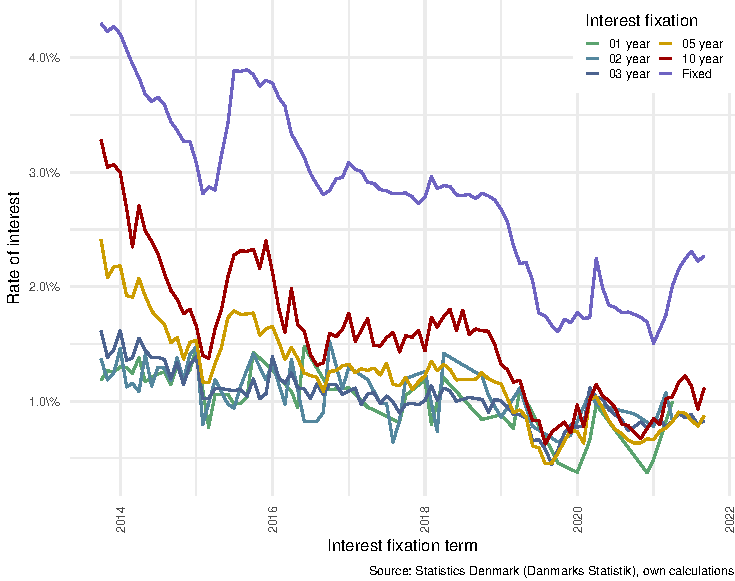
\includegraphics{figures/dst-interestrates-plot-1.pdf}
\caption{\label{fig:dst-interestrates-plot}Danish interest rates}
\end{figure}

\hypertarget{density-plots-using-ggplot2}{%
\subsection{Density plots using ggplot2}\label{density-plots-using-ggplot2}}

ggplot2 offers a wide range of automatic image processing options. Including density plots.

\begin{Shaded}
\begin{Highlighting}[]
\NormalTok{density\_plot\_interest\_rates }\OtherTok{\textless{}{-}} \FunctionTok{ggplot}\NormalTok{() }\SpecialCharTok{+} 
        \FunctionTok{geom\_density}\NormalTok{(}\AttributeTok{data =}\NormalTok{ DK\_yield\_curves\_rates,}
                     \AttributeTok{mapping =} \FunctionTok{aes}\NormalTok{(}\AttributeTok{x =}\NormalTok{ Value,}
                            \AttributeTok{group =}\NormalTok{ Interest\_Fixation,}
                            \AttributeTok{colour =}\NormalTok{ Interest\_Fixation)) }\SpecialCharTok{+}
\NormalTok{    theme\_extra }\SpecialCharTok{+}
\NormalTok{    legend\_top\_right\_inside }\SpecialCharTok{+}
    \FunctionTok{guides}\NormalTok{(}\AttributeTok{col =} \FunctionTok{guide\_legend}\NormalTok{(}\AttributeTok{nrow =} \DecValTok{3}\NormalTok{, }
                              \AttributeTok{byrow =} \ConstantTok{FALSE}\NormalTok{,}
                              \AttributeTok{title =} \StringTok{"Interest fixation"}\NormalTok{))}
\NormalTok{density\_plot\_interest\_rates}
\end{Highlighting}
\end{Shaded}

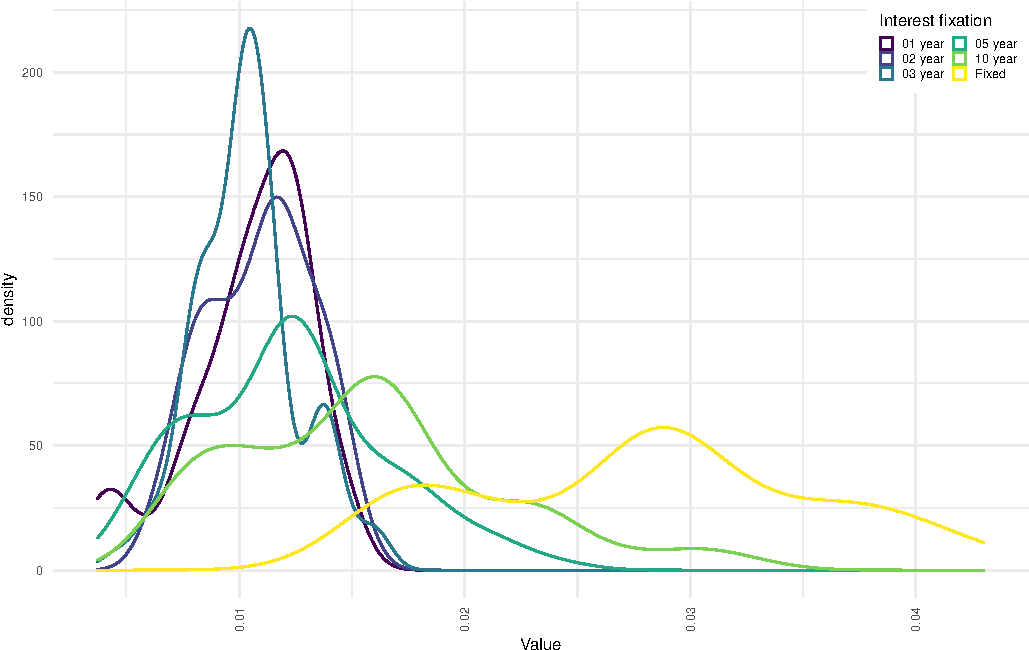
\includegraphics{figures/unnamed-chunk-2-1.pdf}

And the ability to automatically create a tiled ``faceted'' plot of underlying groupings.

\begin{Shaded}
\begin{Highlighting}[]
\NormalTok{density\_plot\_interest\_rates }\OtherTok{\textless{}{-}} \FunctionTok{ggplot}\NormalTok{() }\SpecialCharTok{+} 
        \FunctionTok{geom\_density}\NormalTok{(}\AttributeTok{data =}\NormalTok{ DK\_yield\_curves\_rates,}
                     \AttributeTok{mapping =} \FunctionTok{aes}\NormalTok{(}\AttributeTok{x =}\NormalTok{ Value,}
                            \AttributeTok{group =}\NormalTok{ Interest\_Fixation,}
                            \AttributeTok{colour =}\NormalTok{ Interest\_Fixation)) }\SpecialCharTok{+}
    \FunctionTok{facet\_wrap}\NormalTok{(}\SpecialCharTok{\textasciitilde{}}\NormalTok{Interest\_Fixation) }\SpecialCharTok{+}
\NormalTok{    theme\_extra }\SpecialCharTok{+}
\NormalTok{    legend\_top\_right\_inside }\SpecialCharTok{+}
    \FunctionTok{guides}\NormalTok{(}\AttributeTok{col =} \FunctionTok{guide\_legend}\NormalTok{(}\AttributeTok{nrow =} \DecValTok{3}\NormalTok{, }
                              \AttributeTok{byrow =} \ConstantTok{FALSE}\NormalTok{,}
                              \AttributeTok{title =} \StringTok{"Interest fixation"}\NormalTok{))}
\NormalTok{density\_plot\_interest\_rates}
\end{Highlighting}
\end{Shaded}

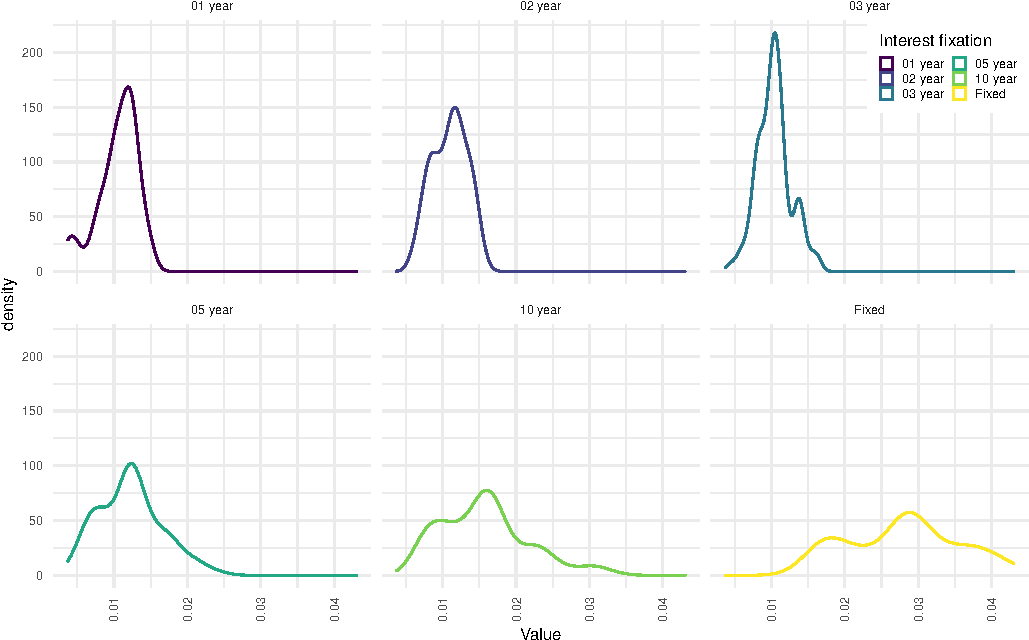
\includegraphics{figures/unnamed-chunk-3-1.pdf}

With minor modifications to the \texttt{aes} (aesthetics) properties, you can automatically change all plots to be filled in for these density plots. The Fill aesthetic is not available for all \texttt{geom}'s, so you will need to investigate the options for the ones that you are interested in.

You can see that I have also modified the number of rows in the legend to 6, to keep the legend narrower - since it overlaps the data in the top right corner. Additional legend options \href{https://ggplot2.tidyverse.org/reference/guide_legend.html}{can be seen here}. The identical legend settings and titles for \texttt{col} and \texttt{fill} prevent duplicate legends from being created. you can test this out by modifying one of the title texts.

The two options \texttt{theme\_extra}, and \texttt{legend\_top\_right\_inside}, are created above in the additional charting options section, and illustrate one way to keep your plotting code a little cleaner.

\begin{Shaded}
\begin{Highlighting}[]
\NormalTok{density\_plot\_interest\_rates }\OtherTok{\textless{}{-}} \FunctionTok{ggplot}\NormalTok{() }\SpecialCharTok{+} 
        \FunctionTok{geom\_density}\NormalTok{(}\AttributeTok{data =}\NormalTok{ DK\_yield\_curves\_rates,}
                     \AttributeTok{mapping =} \FunctionTok{aes}\NormalTok{(}\AttributeTok{x =}\NormalTok{ Value,}
                            \AttributeTok{group =}\NormalTok{ Interest\_Fixation,}
                            \AttributeTok{colour =}\NormalTok{ Interest\_Fixation,}
                            \AttributeTok{fill =}\NormalTok{ Interest\_Fixation)) }\SpecialCharTok{+}
    \FunctionTok{facet\_wrap}\NormalTok{(}\SpecialCharTok{\textasciitilde{}}\NormalTok{Interest\_Fixation) }\SpecialCharTok{+}
\NormalTok{    theme\_extra }\SpecialCharTok{+}
\NormalTok{    legend\_top\_right\_inside }\SpecialCharTok{+}
    \FunctionTok{guides}\NormalTok{(}\AttributeTok{col =} \FunctionTok{guide\_legend}\NormalTok{(}\AttributeTok{nrow =} \DecValTok{6}\NormalTok{, }
                              \AttributeTok{byrow =} \ConstantTok{FALSE}\NormalTok{,}
                              \AttributeTok{title =} \StringTok{"Interest fixation"}\NormalTok{),}
           \AttributeTok{fill =} \FunctionTok{guide\_legend}\NormalTok{(}\AttributeTok{nrow =} \DecValTok{6}\NormalTok{, }
                              \AttributeTok{byrow =} \ConstantTok{FALSE}\NormalTok{,}
                              \AttributeTok{title =} \StringTok{"Interest fixation"}\NormalTok{))}
\NormalTok{density\_plot\_interest\_rates}
\end{Highlighting}
\end{Shaded}

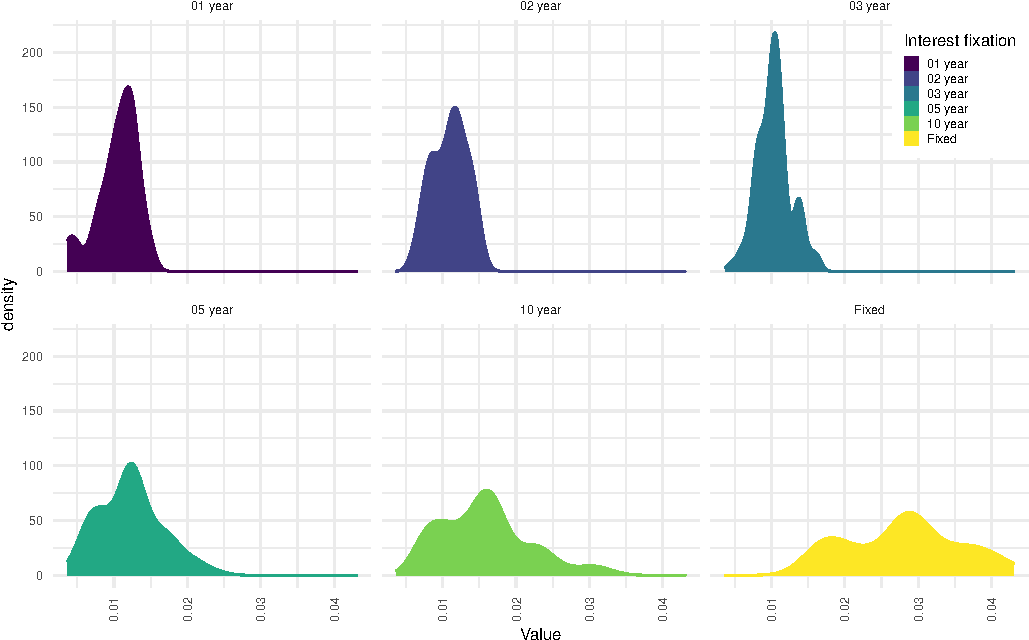
\includegraphics{figures/unnamed-chunk-4-1.pdf}
\newpage

\hypertarget{example-table}{%
\section{Example table}\label{example-table}}

The \texttt{kableExtra} package provides some exceptionally simple quickformatting options for both html and PDF table generation. (\href{https://cran.r-project.org/web/packages/kableExtra/vignettes/awesome_table_in_html.html\#Overview}{Link to explainer page here})

The above sourced interest rate data can be quickly laid out in a table as follows:

\begin{Shaded}
\begin{Highlighting}[]
\NormalTok{pre\_created\_table }\OtherTok{\textless{}{-}}\NormalTok{ DK\_yield\_curves\_rates }\SpecialCharTok{\%\textgreater{}\%}
          \FunctionTok{arrange}\NormalTok{(Interest\_Fixation) }\SpecialCharTok{\%\textgreater{}\%}
          \FunctionTok{spread}\NormalTok{(}\AttributeTok{key =}\NormalTok{ Interest\_Fixation, }\AttributeTok{value =}\NormalTok{ Value)}

\NormalTok{pre\_created\_table }\SpecialCharTok{\%\textgreater{}\%}
  \FunctionTok{kbl}\NormalTok{(}\AttributeTok{caption =} \StringTok{"Table of interest rates over time"}\NormalTok{) }\SpecialCharTok{\%\textgreater{}\%}
  \FunctionTok{kable\_styling}\NormalTok{(}\AttributeTok{bootstrap\_options =} \FunctionTok{c}\NormalTok{(}\StringTok{"striped"}\NormalTok{, }\StringTok{"hover"}\NormalTok{))}
\end{Highlighting}
\end{Shaded}

\begin{table}

\caption{\label{tab:unnamed-chunk-5}Table of interest rates over time}
\centering
\begin{tabular}[t]{l|r|r|r|r|r|r}
\hline
Date & 01 year & 02 year & 03 year & 05 year & 10 year & Fixed\\
\hline
2013-10-01 & 0.01183 & 0.01369 & 0.01613 & 0.02411 & 0.03282 & 0.04302\\
\hline
2013-11-01 & 0.01268 & 0.01185 & 0.01383 & 0.02078 & 0.03044 & 0.04229\\
\hline
2013-12-01 & 0.01252 & 0.01243 & 0.01448 & 0.02172 & 0.03067 & 0.04276\\
\hline
2014-01-01 & 0.01301 & 0.01459 & 0.01615 & 0.02183 & 0.02997 & 0.04208\\
\hline
2014-02-01 & 0.01294 & 0.01124 & 0.01357 & 0.01921 & 0.02680 & 0.04069\\
\hline
2014-03-01 & 0.01245 & 0.01155 & 0.01378 & 0.01909 & 0.02347 & 0.03945\\
\hline
2014-04-01 & 0.01380 & 0.01083 & 0.01550 & 0.02072 & 0.02705 & 0.03826\\
\hline
2014-05-01 & 0.01171 & 0.01405 & 0.01441 & 0.01918 & 0.02486 & 0.03681\\
\hline
2014-06-01 & 0.01209 & 0.01131 & 0.01382 & 0.01788 & 0.02397 & 0.03619\\
\hline
2014-07-01 & 0.01236 & 0.01295 & 0.01383 & 0.01723 & 0.02286 & 0.03656\\
\hline
2014-08-01 & 0.01256 & 0.01288 & 0.01362 & 0.01673 & 0.02114 & 0.03589\\
\hline
2014-09-01 & 0.01145 & 0.01181 & 0.01197 & 0.01510 & 0.01968 & 0.03442\\
\hline
2014-10-01 & 0.01309 & 0.01376 & 0.01334 & 0.01555 & 0.01891 & 0.03366\\
\hline
2014-11-01 & 0.01189 & 0.01186 & 0.01144 & 0.01368 & 0.01763 & 0.03269\\
\hline
2014-12-01 & 0.01272 & 0.01406 & 0.01318 & 0.01514 & 0.01804 & 0.03269\\
\hline
2015-01-01 & 0.01465 & 0.01474 & 0.01387 & 0.01532 & 0.01654 & 0.03083\\
\hline
2015-02-01 &  & 0.00796 & 0.01023 & 0.01168 & 0.01399 & 0.02812\\
\hline
2015-03-01 & 0.00772 &  & 0.01024 & 0.01161 & 0.01373 & 0.02872\\
\hline
2015-04-01 & 0.01061 & 0.01187 & 0.01110 & 0.01328 & 0.01633 & 0.02842\\
\hline
2015-05-01 &  &  & 0.01112 & 0.01465 & 0.01794 & 0.03145\\
\hline
2015-06-01 & 0.01061 & 0.00975 & 0.01099 & 0.01728 & 0.02083 & 0.03419\\
\hline
2015-07-01 & 0.00974 & 0.00938 & 0.01092 & 0.01789 & 0.02276 & 0.03888\\
\hline
2015-08-01 & 0.00983 & 0.01130 & 0.01105 & 0.01758 & 0.02313 & 0.03881\\
\hline
2015-09-01 & 0.01035 &  & 0.01043 & 0.01762 & 0.02309 & 0.03896\\
\hline
2015-10-01 & 0.01427 & 0.01412 & 0.01193 & 0.01770 & 0.02328 & 0.03854\\
\hline
2015-11-01 &  &  & 0.01021 & 0.01576 & 0.02160 & 0.03752\\
\hline
2015-12-01 &  & 0.01188 & 0.01065 & 0.01632 & 0.02399 & 0.03803\\
\hline
2016-01-01 & 0.01271 & 0.01328 & 0.01388 & 0.01653 & 0.02127 & 0.03778\\
\hline
2016-02-01 &  &  & 0.01200 & 0.01513 & 0.01803 & 0.03652\\
\hline
2016-03-01 &  & 0.00975 & 0.01159 & 0.01364 & 0.01602 & 0.03576\\
\hline
2016-04-01 & 0.01084 & 0.01364 & 0.01246 & 0.01468 & 0.01983 & 0.03336\\
\hline
2016-05-01 & 0.00946 &  & 0.01117 & 0.01373 & 0.01669 & 0.03237\\
\hline
2016-06-01 & 0.01477 & 0.00825 & 0.01105 & 0.01246 & 0.01613 & 0.03131\\
\hline
2016-07-01 &  &  & 0.01022 & 0.01225 & 0.01406 & 0.02989\\
\hline
2016-08-01 &  & 0.00824 & 0.01149 & 0.01207 & 0.01313 & 0.02893\\
\hline
2016-09-01 &  & 0.00901 & 0.01058 & 0.01087 & 0.01335 & 0.02803\\
\hline
2016-10-01 & 0.01101 & 0.01521 & 0.01145 & 0.01261 & 0.01594 & 0.02842\\
\hline
2016-11-01 &  &  & 0.01142 & 0.01265 & 0.01564 & 0.02941\\
\hline
2016-12-01 &  & 0.01108 & 0.01058 & 0.01309 & 0.01623 & 0.02955\\
\hline
2017-01-01 & 0.01115 & 0.01296 & 0.01087 & 0.01322 & 0.01767 & 0.03084\\
\hline
2017-02-01 &  &  & 0.01114 & 0.01247 & 0.01522 & 0.03025\\
\hline
2017-03-01 &  &  & 0.00970 & 0.01283 &  & 0.03009\\
\hline
2017-04-01 & 0.00948 & 0.01188 & 0.01063 & 0.01269 & 0.01721 & 0.02911\\
\hline
2017-05-01 &  &  & 0.01074 & 0.01288 & 0.01486 & 0.02903\\
\hline
2017-06-01 &  & 0.00983 & 0.00978 & 0.01229 & 0.01481 & 0.02847\\
\hline
2017-07-01 &  & 0.00979 & 0.01045 & 0.01330 & 0.01555 & 0.02839\\
\hline
2017-08-01 &  & 0.00642 & 0.00992 & 0.01147 & 0.01599 & 0.02811\\
\hline
2017-09-01 & 0.00813 & 0.00827 & 0.00896 & 0.01133 & 0.01430 & 0.02817\\
\hline
2017-10-01 & 0.01051 & 0.01198 & 0.00972 & 0.01207 & 0.01572 & 0.02818\\
\hline
2017-11-01 &  &  & 0.00980 & 0.01102 & 0.01558 & 0.02786\\
\hline
2017-12-01 &  &  & 0.00969 & 0.01168 & 0.01617 & 0.02727\\
\hline
2018-01-01 & 0.01184 & 0.01259 & 0.01004 & 0.01222 & 0.01440 & 0.02779\\
\hline
2018-02-01 & 0.00797 &  & 0.01133 & 0.01348 & 0.01733 & 0.02962\\
\hline
2018-03-01 &  & 0.00735 & 0.01009 & 0.01266 & 0.01648 & 0.02858\\
\hline
2018-04-01 & 0.01203 & 0.01417 & 0.01113 & 0.01321 & 0.01740 & 0.02882\\
\hline
2018-05-01 &  &  & 0.01089 & 0.01277 & 0.01802 & 0.02877\\
\hline
2018-06-01 &  &  & 0.00999 & 0.01184 & 0.01618 & 0.02801\\
\hline
2018-07-01 &  &  & 0.01016 & 0.01191 & 0.01795 & 0.02798\\
\hline
2018-08-01 &  &  & 0.01034 & 0.01189 & 0.01579 & 0.02805\\
\hline
2018-09-01 &  &  & 0.01021 & 0.01193 & 0.01631 & 0.02770\\
\hline
2018-10-01 & 0.00840 & 0.01218 & 0.01017 & 0.01249 & 0.01615 & 0.02816\\
\hline
2018-11-01 &  & 0.01051 & 0.00903 & 0.01195 & 0.01611 & 0.02793\\
\hline
2018-12-01 &  &  & 0.01016 & 0.01169 & 0.01498 & 0.02760\\
\hline
2019-01-01 & 0.00882 & 0.00858 & 0.01002 & 0.01149 & 0.01319 & 0.02674\\
\hline
2019-02-01 &  &  & 0.00948 & 0.01021 & 0.01274 & 0.02565\\
\hline
2019-03-01 & 0.00763 &  & 0.00887 & 0.00901 & 0.01166 & 0.02359\\
\hline
2019-04-01 & 0.01109 & 0.01114 & 0.00881 & 0.00922 & 0.01182 & 0.02202\\
\hline
2019-05-01 &  &  & 0.00853 & 0.00862 & 0.00998 & 0.02212\\
\hline
2019-06-01 &  & 0.00780 & 0.00655 & 0.00608 & 0.00831 & 0.02053\\
\hline
2019-07-01 &  &  & 0.00663 & 0.00590 & 0.00828 & 0.01769\\
\hline
2019-08-01 &  &  & 0.00582 & 0.00453 & 0.00626 & 0.01744\\
\hline
2019-09-01 &  &  & 0.00448 & 0.00460 & 0.00728 & 0.01660\\
\hline
2019-10-01 & 0.00459 & 0.00643 & 0.00576 & 0.00545 & 0.00774 & 0.01609\\
\hline
2019-11-01 &  &  & 0.00723 & 0.00653 & 0.00817 & 0.01716\\
\hline
2019-12-01 &  & 0.00704 & 0.00793 & 0.00746 & 0.00723 & 0.01684\\
\hline
2020-01-01 & 0.00378 & 0.00822 & 0.00772 & 0.00734 & 0.00966 & 0.01772\\
\hline
2020-02-01 &  &  & 0.00786 & 0.00633 & 0.00777 & 0.01723\\
\hline
2020-03-01 & 0.00655 & 0.01075 & 0.01116 & 0.01016 & 0.01004 & 0.01729\\
\hline
2020-04-01 & 0.00969 & 0.00971 & 0.01035 & 0.01038 & 0.01147 & 0.02249\\
\hline
2020-05-01 &  &  & 0.01019 & 0.00940 & 0.01047 & 0.01994\\
\hline
2020-06-01 &  &  & 0.00927 & 0.00829 & 0.01004 & 0.01839\\
\hline
2020-07-01 &  &  & 0.00879 & 0.00754 & 0.00941 & 0.01818\\
\hline
2020-08-01 &  &  & 0.00838 & 0.00716 & 0.00801 & 0.01774\\
\hline
2020-09-01 &  &  & 0.00743 & 0.00658 & 0.00786 & 0.01778\\
\hline
2020-10-01 &  & 0.00888 & 0.00778 & 0.00633 & 0.00726 & 0.01758\\
\hline
2020-11-01 &  &  & 0.00818 & 0.00635 & 0.00675 & 0.01732\\
\hline
2020-12-01 & 0.00373 &  & 0.00762 & 0.00671 &  & 0.01690\\
\hline
2021-01-01 & 0.00487 & 0.00779 & 0.00823 & 0.00662 & 0.00846 & 0.01507\\
\hline
2021-02-01 &  &  & 0.00835 & 0.00742 & 0.00796 & 0.01630\\
\hline
2021-03-01 &  & 0.01072 & 0.00775 & 0.00763 & 0.01020 & 0.01752\\
\hline
\end{tabular}
\end{table}

\hypertarget{interactive-html-plots-with-plotly}{%
\section{Interactive html plots with Plotly}\label{interactive-html-plots-with-plotly}}

A scatter plot with labels on all points can be easily created (some axis limits for the data were necessary below). I also wanted uniform dot sizes and so simply used \texttt{Value\ /\ Value} which returns \texttt{1} for all dot sizes.

\begin{Shaded}
\begin{Highlighting}[]
\FunctionTok{library}\NormalTok{(plotly)}

\NormalTok{a }\OtherTok{\textless{}{-}} \FunctionTok{as.numeric}\NormalTok{(}\FunctionTok{min}\NormalTok{(DK\_yield\_curves\_rates}\SpecialCharTok{$}\NormalTok{Date)) }\SpecialCharTok{*} \DecValTok{24} \SpecialCharTok{*} \DecValTok{60} \SpecialCharTok{*} \DecValTok{60} \SpecialCharTok{*} \DecValTok{1000}
\NormalTok{b }\OtherTok{\textless{}{-}} \FunctionTok{as.numeric}\NormalTok{(}\FunctionTok{max}\NormalTok{(DK\_yield\_curves\_rates}\SpecialCharTok{$}\NormalTok{Date)) }\SpecialCharTok{*} \DecValTok{24} \SpecialCharTok{*} \DecValTok{60} \SpecialCharTok{*} \DecValTok{60} \SpecialCharTok{*} \DecValTok{1000}

\NormalTok{fig }\OtherTok{\textless{}{-}} \FunctionTok{plot\_ly}\NormalTok{(DK\_yield\_curves\_rates }\SpecialCharTok{\%\textgreater{}\%}
\NormalTok{    filter, }\AttributeTok{x =} \SpecialCharTok{\textasciitilde{}}\NormalTok{Date, }\AttributeTok{y =} \SpecialCharTok{\textasciitilde{}}\NormalTok{Value,}
  \CommentTok{\# Hover text:}
  \AttributeTok{text =} \SpecialCharTok{\textasciitilde{}}\FunctionTok{paste}\NormalTok{(}\StringTok{"Interest rate: "}\NormalTok{, Value, }\StringTok{\textquotesingle{}\%\textless{}br\textgreater{}Fixation:\textquotesingle{}}\NormalTok{, Interest\_Fixation),}
  \AttributeTok{mode =} \StringTok{"markers"}\NormalTok{,}
  \AttributeTok{color =} \SpecialCharTok{\textasciitilde{}}\NormalTok{Value, }\AttributeTok{size =} \SpecialCharTok{\textasciitilde{}}\NormalTok{Value}\SpecialCharTok{/}\NormalTok{Value}
\NormalTok{) }\SpecialCharTok{\%\textgreater{}\%}
  \FunctionTok{layout}\NormalTok{(}\AttributeTok{xaxis =} \FunctionTok{list}\NormalTok{(}\AttributeTok{range =} \FunctionTok{c}\NormalTok{(a, b)))}

\NormalTok{fig}
\end{Highlighting}
\end{Shaded}

\hypertarget{htmlwidget-aefe04492b630a916db6}{}

Modifying this plot to return lines, we just need to arrange the data in the correct order to ensure that the lines traced follow the correct pattern.

\begin{Shaded}
\begin{Highlighting}[]
\FunctionTok{library}\NormalTok{(plotly)}

\NormalTok{a }\OtherTok{\textless{}{-}} \FunctionTok{as.numeric}\NormalTok{(}\FunctionTok{min}\NormalTok{(DK\_yield\_curves\_rates}\SpecialCharTok{$}\NormalTok{Date)) }\SpecialCharTok{*} \DecValTok{24} \SpecialCharTok{*} \DecValTok{60} \SpecialCharTok{*} \DecValTok{60} \SpecialCharTok{*} \DecValTok{1000}
\NormalTok{b }\OtherTok{\textless{}{-}} \FunctionTok{as.numeric}\NormalTok{(}\FunctionTok{max}\NormalTok{(DK\_yield\_curves\_rates}\SpecialCharTok{$}\NormalTok{Date)) }\SpecialCharTok{*} \DecValTok{24} \SpecialCharTok{*} \DecValTok{60} \SpecialCharTok{*} \DecValTok{60} \SpecialCharTok{*} \DecValTok{1000}

\NormalTok{fig }\OtherTok{\textless{}{-}} \FunctionTok{plot\_ly}\NormalTok{(DK\_yield\_curves\_rates }\SpecialCharTok{\%\textgreater{}\%}
    \FunctionTok{arrange}\NormalTok{(Date), }
    \AttributeTok{x =} \SpecialCharTok{\textasciitilde{}}\NormalTok{Date, }
    \AttributeTok{y =} \SpecialCharTok{\textasciitilde{}}\NormalTok{Value, }
    \AttributeTok{color =} \SpecialCharTok{\textasciitilde{}}\NormalTok{Interest\_Fixation,}
  \CommentTok{\# Hover text:}
  \AttributeTok{text =} \SpecialCharTok{\textasciitilde{}}\FunctionTok{paste}\NormalTok{(}\StringTok{"Interest rate: "}\NormalTok{, Value, }\StringTok{\textquotesingle{}\%\textless{}br\textgreater{}Fixation:\textquotesingle{}}\NormalTok{, Interest\_Fixation), }
  \AttributeTok{mode =} \StringTok{\textquotesingle{}lines\textquotesingle{}}
\NormalTok{) }\SpecialCharTok{\%\textgreater{}\%}
  \FunctionTok{layout}\NormalTok{(}\AttributeTok{xaxis =} \FunctionTok{list}\NormalTok{(}\AttributeTok{range =} \FunctionTok{c}\NormalTok{(a, b)))}

\NormalTok{fig}
\end{Highlighting}
\end{Shaded}

\hypertarget{htmlwidget-856dd35af42cb78c6f22}{}

\hypertarget{sfc-model-presentation}{%
\chapter{SFC model presentation}\label{sfc-model-presentation}}

Flexible rate mortgage loans: An SFC model of the impact of mortgage credit innovations on Danish balance sheet stability

\hypertarget{abstract}{%
\section*{Abstract}\label{abstract}}
\addcontentsline{toc}{section}{Abstract}

Innovations in mortgage lending options have expounded in recent decades, resulting primarily in a reduction in the initial monthly costs associated with borrowing, and made home ownership possible for socio-economic groups that were previously excluded from the market. These changes have also drastically changed the composition of household balance sheets, both at a micro and a macro level, and the volume of outstanding debt relative to household income expanded aggressively leading up to the global financial crisis in 2007-8. The innovations unfortunately also simultaneously transferred significant risks to borrowers. This paper investigates the present day macroeconomic consequences of the change in composition from fixed- to adjustable-rate mortgage (ARM) debt that occurred in Denmark between 2003 and 2009. A state-of-the-art Stock-Flow Consistent model is adapted to allow for changes in the composition of debt, and to permit shifts in the proportion of debt between fixed-interest and ARM products. The risks to financial stability are evaluated through the imposition of two plausible shocks to the economy: the first is a two percentage point rise in borrowing costs; and, the second is a 20 per cent decline in property prices. The model allows for a clear observation of the transmission channels, and the stocks and flows most at risk, and the results suggest that the expansion of ARM mortgage credit has increased the instability of the household sector. An interesting observation was that a positive net lending response can be misinterpreted as positive developments in the absence of the broader economic context. The paper is supplemented by a new presentation method for SFC model responses, where a cross-section of proportional responses are ranked, ordered and categorised in tabular form.

\hypertarget{sec:fi-fl-sfc-intro}{%
\section{Introduction}\label{sec:fi-fl-sfc-intro}}

Private sector debt continues to be a concern in many developed countries, in particular mortgage debt. Debt levels expanded in most developed countries during the period leading up to the financial crisis, in the household sector this was driven primarily by the extension of mortgage credit (as can be seen in Figure \ref{fig:fl-fi-sfc-lt-debt}, Section \ref{sec:fi-fl-sfc-Ap-A-MtoL}). The proportion of mortgage debt to total debt increased in all countries from around 1960, but accelerated dramatically during the 1990s and 2000s \citep{jorda2017macrofinancial}. That growth was unfortunately not matched by growth in household incomes, and debt-to-income continued to expand for all countries until the great financial crisis in 2007-08 (see Figure \ref{fig:fl-fi-sfc-hh-debt} in Section \ref{sec:fi-fl-sfc-Ap-A-MtoGDP}). In most countries, the supply of credit slowed or even reversed as liquidity in overnight markets dried up during the financial crisis\footnote{It should also be noted that since GDP fell in 2007-08 in most countries, the peak in debt-to-GDP ratios in 2007-08 does not necessarily represent growth in debt, but partly a fall in GDP.}.

The growing debt, particularly relative to income, carries several significant risks to financial stability. These include several demand related risks, such as the future need to deleverage and the associated intertemporal substitution of demand \citep{Justiniano2015, Raberto2012, Seppecher2015}, deterioration of balance sheets and potential risks to refinancing requirements \citep{bernanke2007, scanlon2008, disyatat2011}, and sensitivity of interest payments to rate changes \citep{sheehy2014}. There are also possible contagion effects across financial markets of default (or non-performance on loans), asset price adjustments and possible deterioration of financial intermediary capital positions \citep{DanmarksNationalbank2016a}. As seen in credit-default-swap market during the 2007-08 financial crisis, the possible collapse of liquidity in certain markets can also generate global instability. At a sectoral level there is also the general risk of the accumulation of large imbalances, such as government or foreign deficits, that can take many years to unwind.

While there are a number of parallels between various housing finance systems, the stability of each is unique to a variety of in and out of country conditions. The European Network of Housing Research (ENHR) \citep{lunde2014introduction} found that Political, geographical and institutional factors were not sufficient to explain significant differences in developments across 21 OECD countries since 1989. They \citep[pp.~4]{lunde2014introduction} noted that ``housing finance systems are very specific to each country, reflecting different histories, legal systems, institutions, economic conditions, policies and politics.'' It is therefore necessary to explore the particular dynamics that are at play in each country.

This paper focuses on the Danish system, which makes an excellent country for a number of reasons. Firstly, the Danish housing finance system has been no stranger to innovation, with a number of legislative and product changes introduced since 2003. It is also a relatively small and open economy with strong international trade ties and close ties with the European Union. Thus, a number of parallels can be drawn between the Danish system and several other countries with advanced mortgage financing systems. Denmark is also one of the very few countries that has reliable data for institutional sector balance sheets in granular detail from 1995, and sub-sector level data from 2003. This data allows one to study the problem from comprehensive empirical data. It also allows one to construct a model that integrates the complex interactions and feedback mechanisms of the five institutional sectors that is founded on observable empirical relationships\footnote{In addition, administrative registers make it possible to explore the trajectory of various product ranges in far greater detail, although these are only available after 2009 for mortgage bond debt.}.

In this paper I modify an existing empirical stock flow consistent (SFC) model for the Danish economy first presented by \citet{byrialsenraza2019empirical}. As explained by \citet{godleylavoie2012}, these models maintain strict stock and flow consistency, in the sense that all flows are accounted for in a complete system of accumulations in the stocks of all five major institutional sectors. It attempts to capture the aggregate drivers of macroeconomic interactions as they happen in real time, although it uses \emph{ex post} aggregate accounting values to estimate these relationships.

The completeness of the model requires that some of the variables in the model are passive to changes in others. The choice of the active variables over the passive (residual) variables is determined by a combination of accounting identities and economic theory, in this case, Post Keynesian theory. The grounds for this decision are discussed in Section \ref{sec:fi-fl-sfc-lit}.

Since the household sector is at the core of the analysis in the model, most sectors are passive to changes in the household sector, and it combines the attractive features of econometrics (structural econometric models, SEMs) with path dependency and Post Keynesian behaviours. In the strict sense the model does not demonstrate causality. Rather, it estimates the expected co-movement of certain economic aggregates based on historical evidence and theoretical expectations. These estimates inform several parameters in a medium sized system of equations\footnote{This model has 131 equations, there are thus 131 endogenous variables (including checks) and 78 exogenous. There are in also several equations included as checks and balances, but which do not impact the functioning of the model.}.

The core focus of the investigation in this version of the model is the Danish mortgage system, and the expected macroeconomic consequences of innovations in the mortgage product range offered to Danish borrowers. The model in \citet{byrialsenraza2019empirical} is the most advanced empirical SFC model available for Denmark, and thus provides the best possible point of departure. The model is under continuous development, and there are some limitations imposed by the largely exogenous nature of rates of return (including interest rates) and asset prices. A secondary goal is to identify any potential improvements to the existing model with respect to mortgage credit markets.

The original structure is modified to include a split in household debt between fixed and flexible rate products. This allows for the evaluation of the effects of proportional shifts in credit composition. In particular, to investigate the short-term implications for the accumulation of stocks in the household sector of a shift in the proportion of debt from flexible-interest-rate debt to fixed-interest-rate debt, and vice versa\footnote{By making a simple split in the proportion of debt in flexible and fixed rate instruments, and adjusting the rate of interest on each separately, it offers a relatively simple means by which to incorporate a wide variety of credit market and macro-prudential policy tools into an empirical SFC model - many of which can be achieved via a weighted proportional adjustment of the interest rate on each of the debt types.}. The exogenous nature of rates of return and financial asset prices is both an advantage and disadvantage. On the one hand they allow for specific channels in the model to be highlighted, free of disturbance of from inter-connected markets. On the other hand, it implies that market rates and price fluctuations are not propagated automatically. This makes the overall model results less realistic.

One of the major benefits of the SFC framework is that it allows for path dependent accumulation of imbalances. Although there are some limitations (as discussed below), it is thus possible to fully account for feedback effects from accumulations in selected asset classes, albeit within a simple structure. The analysis that follows may also be of value in the assessment of mortgage financing structures in a macroeconomic framework, and contributes to the growing literature on empirical SFC models.

The remainder of the paper is structured as follows,
Section \ref{sec:fi-fl-sfc-lit} presents a review of the literature, and
Section \ref{sec:fi-fl-rk-dk} provides context for the Danish mortgage market.
Section \ref{sec:fi-fl-sfc-model-features} describes the model, and explains some of the key innovations made in this paper, and
Section \ref{sec:fi-fl-sfc-scenarios} explains the scenarios for shocks applied to the model.
In Section \ref{sec:fi-fl-sfc-simulations} the effects of the shocks are described for each of the scenarios, taken from the perspective of each of the main institutional sectors.
Section \ref{sec:fi-fl-sfc-discussion} contains a discussion of the main observations from the model, and
Section \ref{sec:fi-fl-sfc-conclusion} concludes. The first appendix,
Section \ref{sec:Appendix}, contains a number of additional charts and figures, and the second appendix,
Section \ref{sec:fi-fl-sfc-full-model}, provides a full exposition of the model employed, together with explanations for the major innovations.

\hypertarget{sec:fi-fl-sfc-lit}{%
\section{Literature and theory}\label{sec:fi-fl-sfc-lit}}

\hypertarget{stock-flow-consistent-models}{%
\subsection{Stock flow consistent models}\label{stock-flow-consistent-models}}

Stock flow consistent (SFC) models are a relatively new branch of macroeconomic model, and as mentioned above, are characterised by strict adherence to double entry accounting rules. They resemble structural econometric models, but the expected behaviours that are modelled are typically informed by Post Keynesian theory. \citet{godleylavoie2007}\footnote{The original work has been revised and re-published as \citet{godleylavoie2012}.} is widely regarded as the catalyst for the recent growth in research using the SFC framework, and since 2007 the number of models has grown rapidly.

As noted by \citet[pp.~3]{nikiforoszezza2017}, ``accounting consistency is just one side of the SFC approach, with a demand-led economy and an explicit treatment of the financial side being the other.'' \citet{dossantos2006}, \citet{caverzasi2013}, \citet{caverzasigodin2015} and \citet{nikiforoszezza2017} provide surveys of the literature, each progressively covering the most recent publications. These studies provide a comprehensive review of both the topic and methodological coverage of SFC research. SFC models can be separated into three broad categories; theoretical models, which are typically much simpler and are used for the exploration of theoretical propositions; simulated calibrated models, which are larger models that are constructed to have similar features to real economies, but where the underlying data is constructed for illustrative purposes; and, empirical models, where the entire model is based on real-world data. While each form presents challenges, empirical models face additional challenges with regards availability and reliability of data. Where data is available, the researcher is faced with the challenge of appropriate aggregation.

There are relatively few fully empirical SFC models in the literature, and the number of models for which comprehensive data was available is even lower. The model presented below is an empirical model, based on the one constructed by \citet{byrialsenraza2019empirical}. Unlike many other empirical SFC models, it is constructed from the ground up, rather than adapted from one of the more broadly used \citet{godleylavoie2012} models. This approach mirrors that suggested by \citet{zezza2019design}, where the full complexity of national accounts data is used as the point of departure. The explicit treatment of the financial side entails significant simplification of the wide variety of financial instruments that are available.

Much like many other modelling forms, the complexity of an SFC model has implications for how easily the results can be interpreted. The greater the number of interdependent features, the lower the transparency of transmission mechanisms. In summary of a central banker forum, \citet[pp.~25]{Pill2001} noted that some participants argued that large ``eclectic'' macroeconomic models often ``lack the simplicity, internal consistency and intuitive appeal which are prerequisites for providing good policy advice''. In contrast, others ``suggested that preparing policy guidance in the context of a single model allowed a holistic and rich picture of the economic situation to be obtained.'' This conflict between holistic context and intuitive simplicity was a key part of the decision to keep rates of return exogenous in the present model. It also provides some explanation of the aggregation process. A careful investigation of the size and relative importance of various stocks and flows was conducted to render the model to workable size. Further details regarding the actual aggregation of different categories financial and real flows are provided in Section \ref{sec:fi-fl-sfc-model-features}.

This process requires detailed data, particularly in terms of the balance sheets and flow-of-funds between the institutional sectors. This data is available for very few countries for a long enough time-period to be able to estimate statistical relationships, and Denmark is one of those countries. The model is based on annual data from 1995 to 2017, and there are thus a maximum of twenty two observations in any estimation and the extent to which the model effectively follows the data is comprehensively illustrated in \citet{byrialsenraza2019empirical}.

\hypertarget{post-keynesian-theoretical-foundations}{%
\subsection{Post Keynesian theoretical foundations}\label{post-keynesian-theoretical-foundations}}

The theoretical basis of the model informs the behaviours in and ordering of equations. Since the publication of \citet{godleylavoie2012}'s first edition in 2007, the number of SFC models developed globally has grown exponentially, and due to the Post Keynesian roots of the framework, the bulk of these models could be referred to as Post Keynesian Stock Flow Consistent models (PK-SFC models), PK will henceforth be used refer to the ``Post Keynesian'' school of thought. PK theory is typically juxtaposed with the New Neo-Classical synthesis, or New Keynesianism in order to highlight the points of difference. Such a discussion is beyond the scope of this paper\footnote{For a full discussion of these comparisons the reader is referred to \citet{dow1985}, \citet{dow2001pkm}, \citet{chickdow2001flr} and \citet{chick2003}.}, and a brief summary of the key characteristics of PK systems will need to suffice here, with a special focus on those parts used to inform the model below.

In terms of the trajectory of the economy, PKs typically reject the notion of a long run equilibrium in favour of path dependency, and argue that present decisions and institutional structures materially change the nature of the economy in the future. For the present model, this is reflected in the focus on short to medium term (typically the first period or two after a shock, but up to approximately 5 years). They argue also that the economy is significantly more complex than the sum of its parts \citep{chick2003}, and sometimes liken it to an organic entity, or the complex interactions of an ecosystem. Economic trajectories can therefore be altered by active intervention and long term historical averages are therefore not predictive of future events. This is reflected in the model below by a lack of long-run mean reversion or stabilising elements in the model. The most significant omission relative to mainstream literature is the inter-temporal optimisation of household consumption. There are no utility functions, and there is no long-run or inter-temporal optimisation of behaviour.

For economic policy concerns, the implication is that financial and social imbalances cannot self-correct (at least not without significant social, political or economic consequences), and market mechanisms are not able to manage these issues automatically. To the contrary, unchecked imbalances that are perpetuated by market structures are problematic. Just as the accumulation of poor quality private debt prior to the 2007-08 GFC proved to be.

PKs often refer to \citet{keynes1937}, who stated that the future is fundamentally uncertain. It is therefore crucial to understand the economy as it presently stands, and to have some idea of what future economic conditions are desirable. It should thereafter be possible to actively plan for and develop a desirable future economic landscape, without the need for projections of the distant future, or acceptance of any long-run equilibria or natural rates. From a modelling perspective it is therefore not necessary that a model be stationary in order to be useful, it is more important that it should be representative of the present reality.

In terms of the sequence of events inside PK models, they emphasise the importance of demand (or rather effective demand\footnote{Intended here to include both consumption and investment, as explained by \citet{keynes1937}. A slightly broader definition than \citet[pp.~73]{Smith1776}'s effectual demand, which refers to commodity purchase, but with a very similar line of reasoning, where in Smith's commodity markets buyers with the capacity to pay for a good ``may be called the effectual demanders, and their demand the effectual demand; since it may be sufficient to effectuate the bringing of the commodity to market. It is different from the absolute demand. A very poor man may be said in some sense to have a demand for a coach and six; he might like to have it; but his demand is not an effectual demand, as the commodity can never be brought to market in order to satisfy it.''}) in the economy, and are predominantly demand driven rather than supply driven - although, more recent works have put more emphasis on supply side constrains \citep{skott2008supplyside}. Keynes's animal spirits and short term expectations drive investors to either increase or decrease investment. This is also related to the PK theory of an endogenous demand and supply of money in the economy. The demands of possible borrowers are tested against credit worthiness and all viable demand for credit is (or can be) accommodated by the banking sector. New lending creates new money, and therefore the demand for investment funding drives the growth in money. In this model, this analogy is applied to the household sector in that the demand for new housing investment drives the demand for mortgage credit.

There are several estimated equations in the model, and the motivations for each are discussed in a full presentation of the model in Section \ref{sec:fi-fl-sfc-full-model}, in the appendix. The structure of the estimated equations are informed by PK and country specific literature, and refined to reflect the reality of the data.

\hypertarget{credit-markets-and-global-financial-conditions}{%
\subsection{Credit markets and global financial conditions}\label{credit-markets-and-global-financial-conditions}}

From a broader international perspective, the period leading up to the crisis has been called ``the great moderation'' (as noted by, \citet[pp.~28]{Buttiglione2014}) and was an extended period of unprecedented economic growth and apparent stability of financial markets. As noted by \citet{englund1999}, this was accompanied by the relaxation of lending requirements and credit worthiness checks, and as \citet{scanlon2008} identified, rising property prices and expectations of capital gains. There was a gradual reduction of interest rates, and the cost of borrowing (the long-run cost of capital falling steadily from the 1970s). According to \citet{scanlon2008}, a simultaneous development on a global scale was an increased belief in the market mechanism, extensive privatisation and deregulation of financial markets\footnote{One such development in Denmark was the 1993 relaxation of home equity extraction laws \citep{Andersen2019}.}. The onset of the global financial crisis (GFC) later revealed significant flaws and systemically risky interdependencies between markets. Even though the initial effects were felt by all countries, the effects, both in terms of intensity and real economic and financial trajectories, differed greatly. \citep{lunde2014introduction}

In the post-crisis period, there have been significant changes to the regulatory landscape, and the extent of mortgage lending has slowed or reversed in many countries. At the height of the crisis, liquidity in key financial instruments, particularly credit default swaps, dried up almost instantly \citep{danmarksnationalbank2008}. Ultimately this triggered quantitative easing (QE) policies in both the USA and Europe, with the Fed and the ECB buying immense quantities of financial assets and market-making with the assistance of larger banks. On the regulatory front, banking prudential and capital adequacy requirements were tightened significantly. The period from 2009 to 2018, while not as extreme as the period preceding the crisis, has however, continued to show strong growth in property prices, with more than half of the OECD countries in the sample showing year-on-year growth rates of over 2\%, as can be seen in \ref{tab:oecd-house-price-table}.

US and European QE policies also led to excess liquidity in global financial markets. The low short-term rates have gradually resulted in record low long-term rates of return, placing added pressure on fund management and investment companies to search for yield in unconventional investments\footnote{Where performance guarantees have been provided, such as for defined benefit pension schemes, some institutions face negative spreads and the risk that they might not be able to foot the bill at the end of the day. Now in 2019, eleven years after the financial crisis, \citet{ECB2019} announced, on 12 September 2019, a further reduction of ECB deposit facility rates to \(-0.5\%\), and the marginal lending facility to remain at \(0.25\%\). In addition, net purchases of financial assets will begin again in the ``asset purchase programme (APP) at a monthly pace of €20 billion as from 1 November''.}. These policies and other commitments by European central banks and the ECB have contributed significantly to persistent low interest rates in market based mortgage lending systems. While the rate of growth in the level of debt relative to income appears to stabilised in many countries, the magnitude of household debt continues to expand. The risks associated with this debt depend not only on the magnitude of the debt, but also very strongly on its composition.

A correlated development has been the expansion of the product range offered by mortgage lenders. Leading up to 2007, innovations were made to almost every aspect of mortgage lending, and the vast majority of these changes have contributed to a reduction in the initial payments on mortgages for the borrower. According to \citet{scanlon2008}, while the innovations were different according to each specific country, some broader characteristics were similar across developed nations. Two key aspects to these innovations were that they made initial payments on mortgages cheaper, and secondly, they increased the flexibility and range of options available, and thus transferred significant elements of risk to the borrower. \citet{andre2016household} also explains that house price bubbles are often related to periods of financial de-regulation, and highlights the introduction of interest-only (periods without capital repayments) loans in Denmark in 2003 as an example.

These international developments were not applied uniformly to all countries, or even in specific geographical areas. \citet{lunde2014introduction} found, rather surprisingly, that in contrast to a geo-political grouping, for example with other Scandinavian countries, Denmark was closer to Finland, Poland and Russia in terms of real economic and housing financing conditions after the 2007-08 financial crisis. An additional point was that the introduction of adjustable rate mortgage (ARM) products introduced a small but significant possibility of systemic risk to the Danish mortgage system\footnote{In particular, they referred to potential for market failure through liquidity risks for products with 30 year loan guarantees but with interest reset each year. \citet{lunde2014introduction}}. ARMs were first introduced in 1996, but and are just one of several innovations that were introduced to the Danish market.

Affordability of housing also became a prominent issue and tax incentives for interest payments on mortgages were common. According to \citet{scanlon2011}, real house prices in Denmark fell 14.9\% from the peak in 2007 to Q4 2008. House prices rose in all OECD countries from 2000 to 2007\footnote{Data for OECD countries for the periods 2000 - 2007, 2007 - 2008, and 2008 - 2018 can be seen in Table \ref{tab:oecd-house-price-table}, in Section \ref{sec:fi-fl-sfc-Ap-A-OECD-house-prices}.}, with Slovakia (22.41\% year-on-year (yoy)), Ireland (16.65\% yoy), Estonia (15.89\% yoy), Hungary (13.52\% yoy) and Latvia (11.22\% yoy) as the most extreme examples, while Denmark rose at 3.11\% yoy. From 2007 to 2009, house prices stabilised in most countries, and collapsed in a few with Estonia (-17.06\% yoy) and Ireland (-12.57\% yoy) showing the largest collapses. As noted above, Danish house prices reached a trough in Q4 2008 at -14.9\%.

The asset and property price bubbles and collapses of recent years appear therefore to be closely related to developments in credit markets, and as is briefly explained below, the over-extension of private balance sheets and the risk of significant declines in property prices (the bursting of a bubble) could have serious consequences for both individual borrowers and the broader economy. Some of the key credit market innovations that occurred are discussed in the next section, together with some of their main advantages and disadvantages.

\hypertarget{key-innovations-and-developments-in-product-scope}{%
\subsection{Key innovations and developments in product scope}\label{key-innovations-and-developments-in-product-scope}}

Amongst the most common innovations noted by \citet{scanlon2008} included the following. The introduction of flexible-interest rates, and a variety of length of interest rate fixation periods. The introduction of interest-only periods, where repayment of capital or principal are postponed temporarily. Full term interest-only loans, with the principal payable on maturity - these are sometimes linked to investment vehicles designed to accumulate greater capital than the amount contributed (i.e.~with an expected positive spread above the rate of interest). Longer terms of debt, some up to 50 years. Reduced up-front cash (or own) contribution requirements. Increased percentages allowed to be allocated to bond financing, typically at a significantly lower interest rate than would otherwise be available from a bank. Exceptionally low interest rate levels have also seen some innovations in terms of price. Zero-interest 20 year fixed-rate loans as well as negative interest rate flexible-rate (ARM) bonds are at the time of writing available in the Danish market.

Some of the key drivers of these innovations were, as noted by \citet{Alpanda2017}, the availability of new technology, which permitted significantly more complex products to be managed effectively. Government deregulation, and the associated greater market orientation. Rising asset prices and problems with housing affordability. In the post-crisis period, innovations have been driven by some additional factors, including record low interest rates and quantitative easing. Interest rates in developed economies, particularly northern Europe, have been set to record low levels. This has had the dual impact of reducing the cost of borrowing and significantly reducing lender revenues.

\hypertarget{advantages-of-innovations}{%
\subsubsection{Advantages of innovations}\label{advantages-of-innovations}}

The advantages of these innovations have been felt most by borrowers, particularly those groups of borrowers that were previously unable to afford initial payments on home loans \citep{scanlon2008}. As mentioned above, mortgage repayments are in many countries now more affordable in the short term. The flexibility of repayment options has made it possible for borrowers to structure their mortgages according to their expected cash flow requirements, this is especially helpful for borrowers with irregular incomes.

The introduction of interest-only periods, allow borrowers that have limited capacity to change their income levels, particularly the elderly, to maintain a stable standard of living \citep{scanlon2008} - in effect consuming part of their home equity without the need to liquidate the asset. Interest-only periods also allow younger families to absorb temporary increases in living costs, without necessitating the sale of the family home. For example the cost of children, education, or other foreseeable and unforeseeable expenses.

The lengthening of the term of mortgage debts also reduces payments for the full term of the debt, making housing more accessible to groups that would otherwise not have been able to afford it. More sophisticated investors also have the opportunity to benefit from the innovations, where in very low interest environments, they might be able to borrow and invest at higher rates of return than the cost of borrowing. Unfortunately these advantages come with a cost.

\hypertarget{disadvantages-of-innovations}{%
\subsubsection{Disadvantages of innovations}\label{disadvantages-of-innovations}}

The disadvantages described below are considered as compared with a standard fixed-rate annuity mortgage. In general, the innovations in mortgages place significantly greater onus on the borrower to fully understand the product that they choose to take. Several of the benefits described above are also only true for the initial stages of the debt contract, as principal repayment is often built into later stages. These products also introduce additional risk in several forms, including interest rate risk, credit risk, market risk and significant potential opportunity costs - each will be discussed briefly below.

\emph{Interest rate risk}\newline
Perhaps the simplest and most direct effect, which would not be felt by a fix interest rate borrower, is that flexibility of interest rates expose the borrower to future increases in interest expenses, and therefore negative effects to disposable income if interest rates rise.

\emph{Credit risk}\newline
Interest-only periods may reduce monthly outlays, but they also prevent the accumulation of equity by the borrower. This means that there is less of a buffer, making them more sensitive to negative shocks. Negative shocks may include an increase interest rates, the loss of income, illness of self or family members, breakdown of relationships (possibly divorce) or a fall in property prices.

\emph{Market risk}\newline
Borrower solvency is determined on the basis of outstanding debt relative to the value of the property held as collateral, or loan-to-value (LTV) ratio. In the case of property price declines, traditional borrowers would have built a buffer to absorb a decline in collateral value. By contrast, the lack of equity accumulation for interest-only borrowers means that the outstanding debt would not have fallen relative to collateral. Any borrowers with LTVs close to the limit would risk falling into negative equity, and possibly insolvency. \citet{scanlon2011} found that the groups that were most likely to be negatively affected in a crisis were those who had withdrawn equity (potentially via refinancing), or those who had bought close to the top of the market - resulting in high loan-to-value ratios and increased probability of falling into negative equity.

\emph{Opportunity cost}\newline
Taking Denmark as an example, the borrower is endowed with several rights, one of which is that any mortgage bond is callable at any time, and at which time, the borrow can choose to either pay the remaining par value of debt, or to repurchase the same (or similar) bond sold at time of borrowing. What this means is that if interest rates rise after the date of borrowing, there is an opportunity for mortgage borrowers to settle their debt at a significantly reduced capital value. This reduction of debt can also be accomplished by refinancing at a later stage if interest rates were to rise sufficiently to outweigh the costs of refinancing. Borrowers with flexible rate mortgages lose this opportunity, since interest rates on flexible rate bonds are reset more frequently basis, and thus price adjustments are negligible.

In summary, the increased complexity introduced by innovations requires the borrower to have a more sophisticated knowledge of financial matters and to take on more responsibility for the security of collateral and repayment of capital. As has been reported by \citet{scanlon2008}, it is doubtful whether most borrowers are sufficiently equipped to deal with these challenges. Where they do not have sufficient knowledge or skill, households become dependent on financial advisers and service providers to ensure that they have the most appropriate products.

\emph{The credit-asset-price virtuous cycle}\newline
The self-reinforcing cycle of ease in credit markets and growth in asset prices is well documented. \citet{Bernanke1999a} and \citet{disyatat2011} explained this in the context of the financial accelerator, rising property, and asset prices more generally, incentivise borrowing via balance sheet improvements and positive sentiment. In some cases borrowing is speculative, in order to benefit from the rising tide. Low interest rates and greater ease of access to mortgage debt simultaneously increase the pool of participants that demand assets, driving prices progressively higher. This virtuous cycle is mirrored by a similar decline in property prices and availability of credit on the way down. Conditions in credit markets and asset prices are thus difficult to separate.

\hypertarget{sec:fi-fl-rk-dk}{%
\section{Mortgage credit in Denmark}\label{sec:fi-fl-rk-dk}}

As mentioned above, the Danish mortgage lending market has also experienced a number
of the innovations, and is a particularly interesting case due
to a relatively unique approach to mortgage lending.
The system is characterised by what is called the balance principle, which \citet{laustsen2009}
describes as a traditional fund matching principle for mortgage lending. Denmark is
unique in that this traditional principle has been respected for over 200 years. As
noted by \citet[pp.~1]{laustsen2009}, it results in ``Transparent pricing in the form of a direct
transfer of market-based prices to the individual borrower and market-based prepayment
terms. And to the issuer: Limited and transparent risks.''\footnote{The mitigation of risk includes differences in term structure of assets
  and liabilities, refinancing risk, option risk across variations of bond type,
  liquidity risk, foreign exchange risk, and interest rate risk. The instruments issued
  include SDOs (særligt dækkede obligationer, covered bonds), SDROs (særligt dækkede
  realkreditobligationer, covered mortgage bonds) or ROs (traditionelle realkreditobligationer,
  traditional mortgage bonds). \citep{laustsen2009}} As noted by
\citet[pp.~2]{haldrup2017}, a mortgage deed in Denmark is a ``money-creating debt contract'', but in
Denmark, this is financed from the existing money stock\footnote{Another important consideration is that mortgage bond financing is only
  available for a portion of the debt, depending on the nature of the property, and the
  nature of the purchase. See \citet{danske2017danish} and \citet{nykredit2018} for a detailed description
  of the covered bond and covered mortgage bond market in Denmark. Further information is
  available on similar Nordic products in \citet{danske2017nordic}.}.

These stable mortgage lending and covered bond markets have, since 1996, experienced
a number of product\footnote{2003, loans with interest-only (IO) periods. 2004, loans with interest
  rate caps and adjustable rate mortgages (ARMs, or floating-to-fixed rate options). 2007, ratchet coupons.}, operational\footnote{2006 additional auctions in March and September. 2014, additional
  auction in June.} and
legislative\footnote{English translations of financial regulation acts are available
  from \url{https://www.dfsa.dk/en/Rules-and-Practice/Translated_regulations/Acts}, however, there
  have been additional alterations since then. Legislation permitting multiple purpose use
  of mortgage debt against fixed property was introduced as early 1993.} innovations. The IMF \citep{sheehy2014} conducted an
assessment of the risk related to the structure of mortgage debt in Denmark in 2014,
and found that there was a strong shift after 2003 towards flexible rate mortgages. This
strong shift was warned against, and the financial supervisory authority, in collaboration
with banks, began to reduce the exposure of HH to flexible rate products. While the problem
was recognised, the level of flexible rate mortgage bond exposure remains high, with roughly 70\%
of outstanding mortgage debt to be repriced within the next five years. As in most other countries,
the rights and protections of the borrower have been enhanced by several additional legislative
changes\footnote{As noted by \citet[pp.~12]{laustsen2009}, these include 1.) EU Capital Requirements
  Directive (CRD) and the UCITS Directive together set out the EU's
  definition of covered bonds. EU Directive 2006/48/EC of 14 June 2006 relating to the taking
  up and pursuit of the business of credit institutions, and EU Directive 2006/49/EC of 14 June 2006
  on the capital adequacy of investment firms and credit institutions (dubbed the Capital
  Requirement Directive -- CRD).
  2.) Executive Order no 718 of 21 June 2007 -- Executive Order on bond issuance, balance
  principle and risk management.
  3.) The par rule, applied from the final report of the committee on business and commerce of
  the Danish parliament prior to the adoption of the act in May 2007. Prepayment of loans funded
  by SDO issuance must ``\ldots{} take place on reasonable terms and according to a practice that does
  not deviate from the terms applicable to housing loans today. this means that prepayment may
  take place by way of a buyback of the underlying bonds or at a price that does not deviate
  significantly from par, in part out of consideration for ARMs-like products. If a loan is not
  linked to listed bonds, prepayment may take place at par.''
  4.) Act no 577 of 6 June 2007 -- Act amending the Financial Business Act and various other acts
  (SDOs) -- and pertaining explanatory notes and final report.}, several of which have been implemented in order to keep up with
the rapid innovations in mortgage markets described above.

\hypertarget{composition-of-danish-mortgage-debt}{%
\subsubsection{Composition of Danish mortgage debt}\label{composition-of-danish-mortgage-debt}}

The composition of Danish real estate debt is rather complex to measure in its entirety,
as there is a strong possibility that first-time
home buyers will take an additional bank loan against their physical property for
approximately 15\% of the market value. In the data below, this portion of the debt
is not included, and thus, the total debt outstanding represents a somewhat lower total
than that official measures of total household debt used in the model that follows\footnote{The data used for the model is aggregate data sourced from Eurostat, and does not provide the level of granularity presented here. It does, however, separate long- and short-term debt, and the majority of bank loans for the purpose of property purchase are included in the long term category. These bank loans are also flexible-interest rate products, and could thus be included in the flexible portion of mortgage debts outstanding. Unfortunately we do not have data that makes it possible to identify this debt separately, and thus it is excluded in the present section.}.

The following data are constructed from administrative registers, which allows for a more granular view
of recent developments than is typically available. The actual data are significantly more detailed
than that presented here, but further disaggregation makes visual comparison difficult due to the relative
(in)significance of some subcategories of debt. The two main dimensions on which we are interested in
splitting mortgage debt are the term remaining on the debt and the length of time for which the interest rate
is fixed (referred to as `\emph{interest fixation}' below). The interest fixation for ARM products shortened dramatically
leading up to 2007, but has lengthened somewhat since the crisis, Unfortunately, the detailed micro-data is
only available after 2009, which means that details during the expansion of mortgage debt are not available.

At a national level, the total level of debt split by interest fixation, can be seen in Figure \ref{fig:debt-composition-dk-all-term}. The first thing to note is that the nominal level of mortgage debt, in panel (a), has continued to rise throughout the period from 2009 through 2017.

\begin{figure}[H]
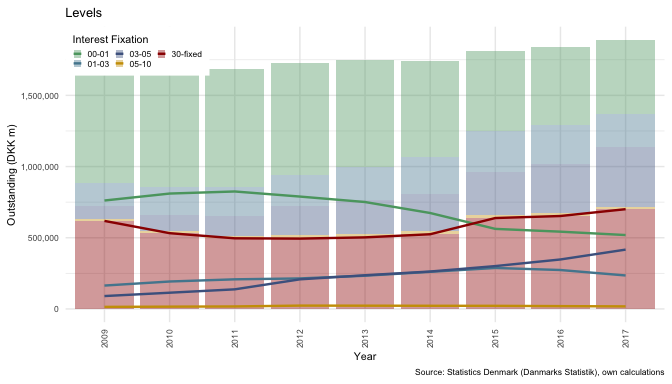
\includegraphics[width=0.5\linewidth]{figures/unnamed-chunk-8-1} 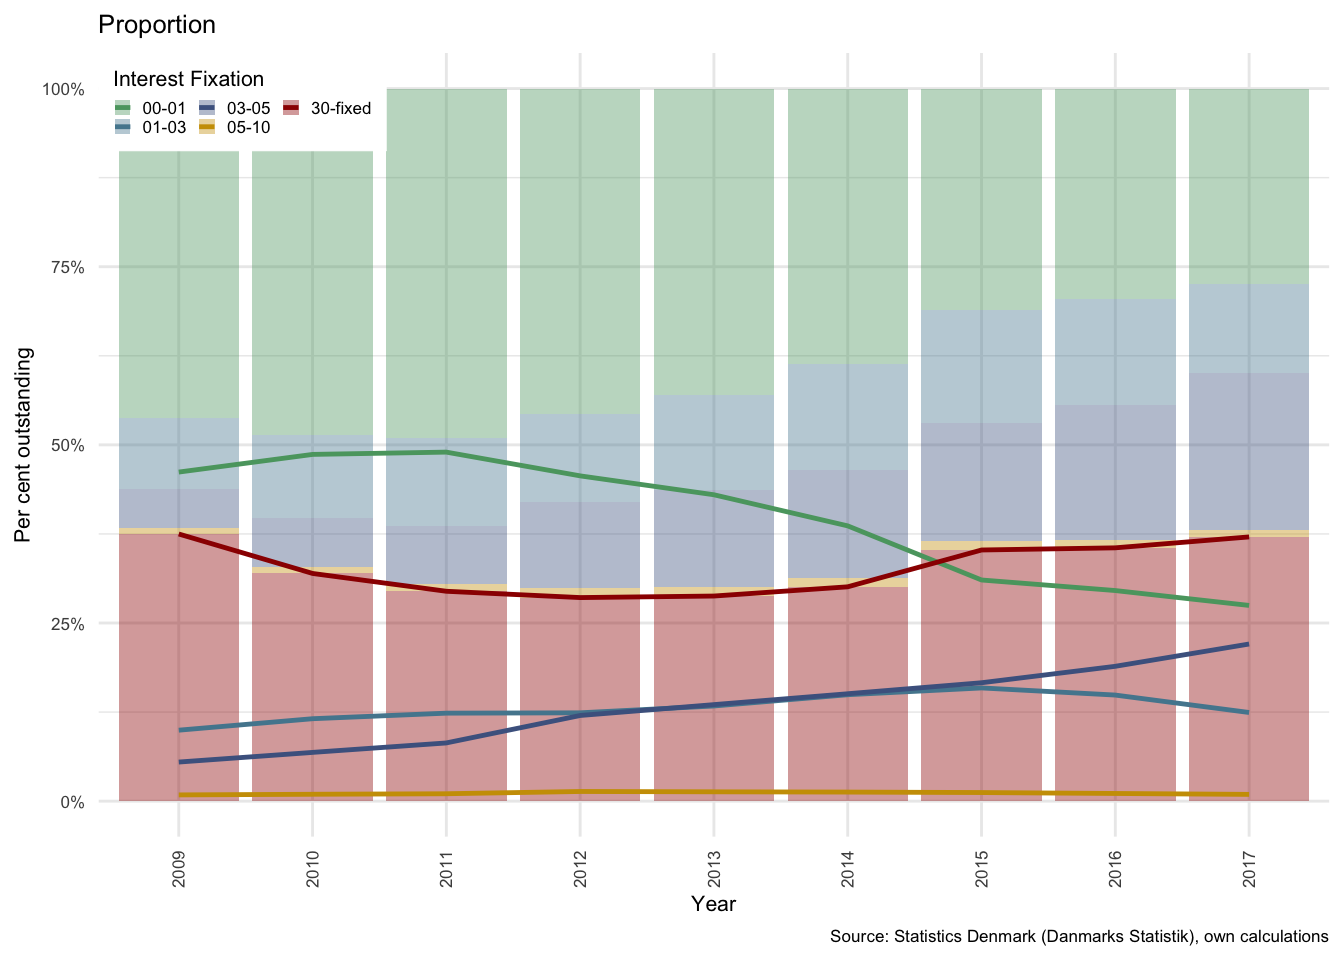
\includegraphics[width=0.5\linewidth]{figures/unnamed-chunk-8-2} \caption{Mortgage debt in Denmark: All term lengths}\label{fig:unnamed-chunk-8}
\end{figure}

This can also be considered in proportional terms, where the percentage of debt outstanding in
each category is easier to read. As can be seen in Figure \ref{fig:debt-composition-dk-all-term} part (b) above,
the 30-fixed category, which covers all fixed rate products\footnote{Due to the choice of data categorisation in the real-kredit register from Statistics Denmark, all contracts with fixed-interest are recorded as a 30 year fixation period.}, was still in decline as a proportion of total outstanding mortgage debt from 2009 to 2012.

The most concerning factor, and one raised by \citet{sheehy2014}, in an IMF stability report, was the growing proportion of debt that would reprice within relatively short intervals. At the start of 2011, debt with an interest fixation of less than and up to 1 year (the green line) was by far the largest contributor. This was recognised by both domestic and foreign prudential regulators as a risky development, and in collaboration with the banking sector and real estate finance companies a variety of measures were implemented to reverse this trajectory. \citep{sheehy2014}

These patterns can further be decomposed into a variety of term structures.
As can be seen from Figure \ref{fig:debt-composition-dk-det-term}, the
proportional composition of debt is significantly different for each of the
term groupings\footnote{Debt is separated by term to maturity of between 0
  and 10 years, from 10 to 20 years, from 20 to 25 years and those with a term
  greater than 25 years.}. We will not explore this too deeply, as the
relative importance of each category varies dramatically.

\begin{figure}
\centering
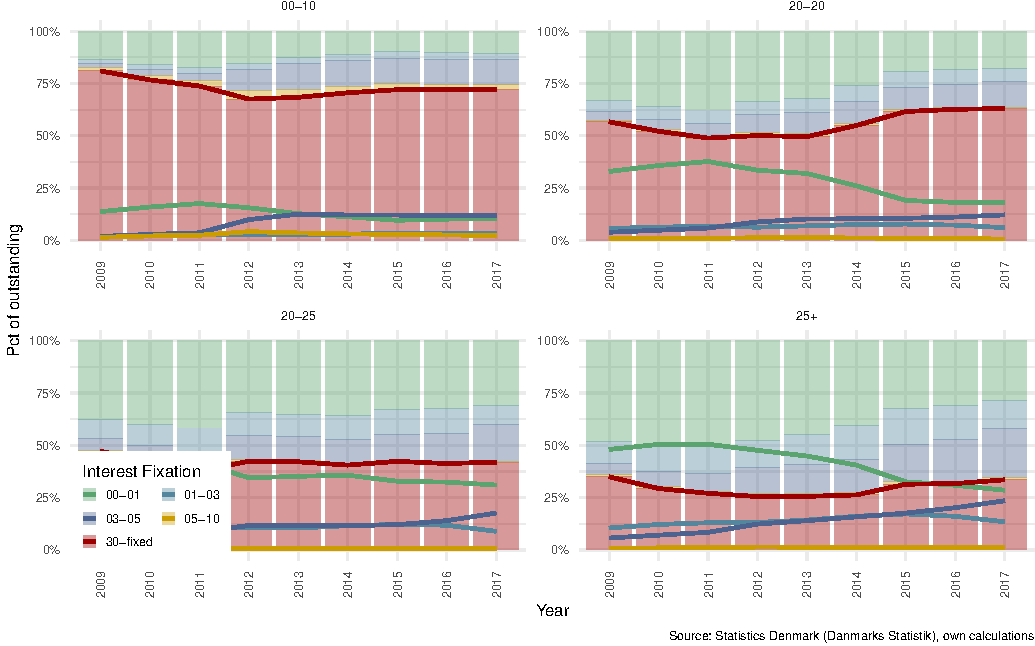
\includegraphics{figures/debt-composition-dk-det-term-1.pdf}
\caption{\label{fig:debt-composition-dk-det-term}Composition of mortgage debt in Denmark: Split by term}
\end{figure}

Figure \ref{fig:debt-values-dk-det-term} illustrates the total outstanding debt in each of the term categories, it can quite easily be seen that by far the largest portion of debt has a term to maturity of over 25 years. In Denmark, the maximum term for which mortgage debt can be acquired is 30 years, thus all debt in this category in each year was issued under five years prior to the year in question. Roughly only one sixth of all outstanding mortgage debt has a term to maturity of less than 25 years.

Of the debt with greater than 25 years to maturity, it can be seen from Figure \ref{fig:debt-composition-dk-det-term}, that only approximately 30\% of this outstanding debt has an interest fixation period of longer than 5 years. This together with approximately half of the other 15\% results in a total of just over 37\% of all outstanding mortgage bond debt. This means that the remaining 63\% of mortgage debt will adjust together with interest rates. The outstanding mortgage bonds will also adjust in price, which effectively means that in the event of an increase in interest rates, nominal debt outstanding will remain fairly constant for the 63\% that has flexible interest products, and debt service costs will rise commensurate with the rise in rates. The aggregate opportunity cost related to capital adjustments for borrowers in this case is potentially very large.

By 2017, the proportion of debt with an interest fixation period of 1 year or less had fallen to approximately 25\% of all outstanding debt. A significant improvement from just under 50\% for 2010 and 2011.

\begin{figure}
\centering
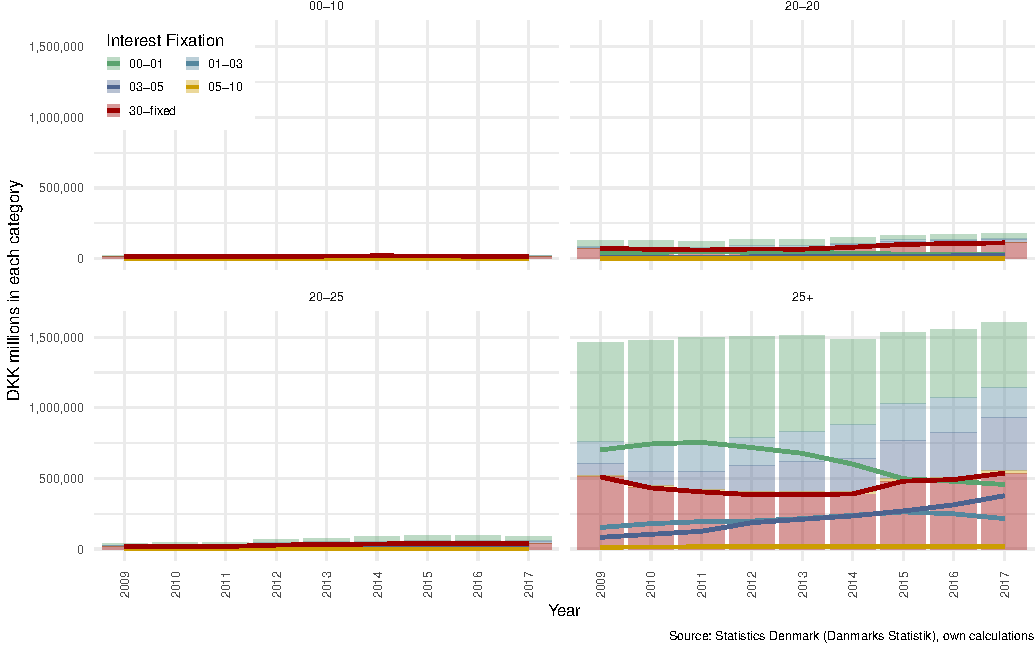
\includegraphics{figures/debt-values-dk-det-term-1.pdf}
\caption{\label{fig:debt-values-dk-det-term}Levels of mortgage debt in Denmark: Split by term}
\end{figure}

Based on the distribution that can be seen in Figure \ref{fig:debt-values-dk-det-term} above, the remainder of the paper uses a much simpler term and interest fixation categorisation. In order to capture all long term debt, all outstanding debt with a term longer than 10 years is included in long term debt, while all shorter terms maturity are included in the short term category. Similarly, interest fixation periods of less than 10 years are included in the short fixation period category, of which the overwhelming majority is fixed for less than five years. All interest fixation periods of longer than 10 years are included in the fixed-interest category. Because the level of mortgage debt with a shorter term is so low (largely irrelevant), this additional categorisation is dropped. Any shorter term mortgage debt is also likely to have similar characteristics of longer term debt that has short interest fixation periods. As such, it is assumed that the only fixed interest debt held by HH is held in the form of mortgage debt. It is therefore possible to categorise all debt in terms of the ``interest fixation'' dimension.

This is supported by Figure \ref{fig:debt-composition-dk-simp}, where the proportion of debt in the shorter term category is essentially negligible in comparison with the longer term outstanding portion.

\begin{figure}
\centering
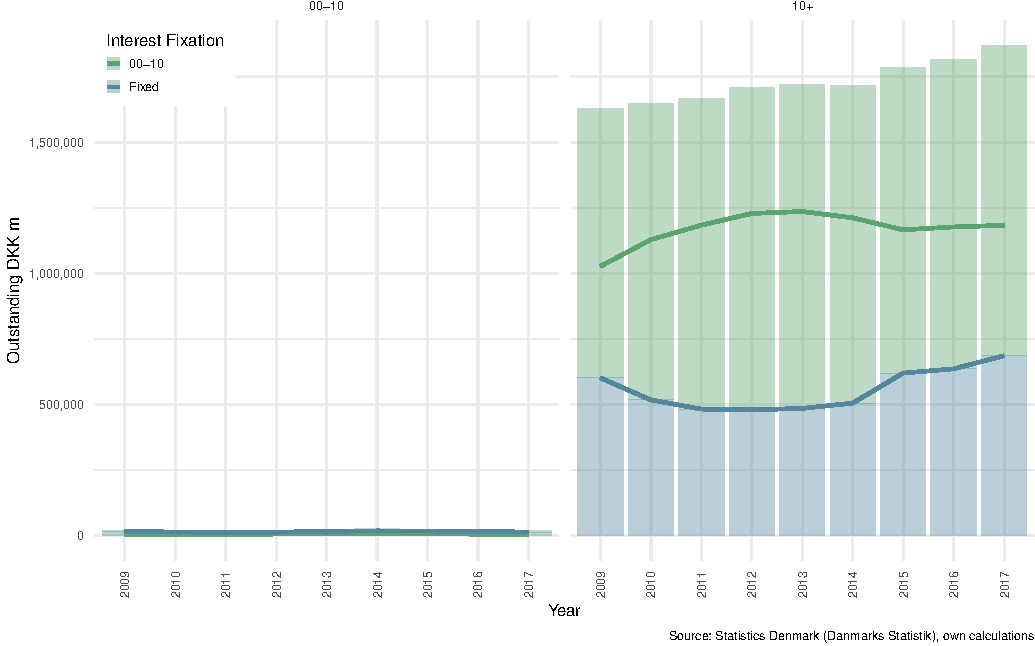
\includegraphics{figures/debt-composition-dk-simp-1.pdf}
\caption{\label{fig:debt-composition-dk-simp}Composition of mortgage debt in Denmark: Simplified, panels by term}
\end{figure}

Figure \ref{fig:debt-composition-dk-simp} shows the nominal outstanding amounts in the short and long term to maturity categories. As can noted above, the short-term-to-maturity debt to the left is of negligible interest for the analysis that follows, and so most of the figures below focus purely on the long term-to-maturity (10+ category) to the right.

Figure \ref{fig:debt-composition-dk-simp-term}, part (a), reflects the relative proportions of fixed and flexible-interest fixation periods in each interest fixation category. The debt with interest-fixation periods of less than 10 years will be referred to as adjustable rate mortgages (ARMs) or flexible-rate mortgages below.

\begin{figure}[H]
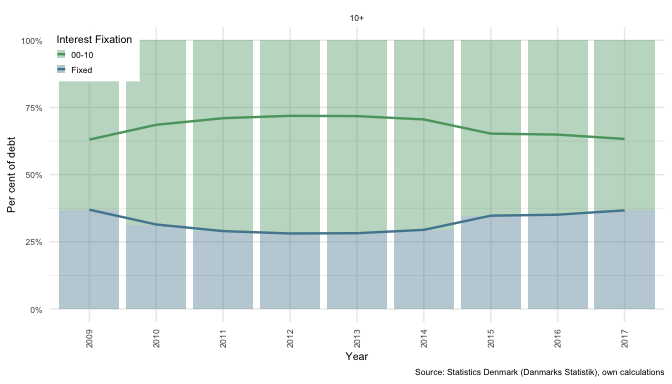
\includegraphics[width=0.95\linewidth]{figures/debt-composition-dk-simp-term-1} \caption{Outstanding mortgage debt and interest payments: Term of 10+ years}\label{fig:debt-composition-dk-simp-term}
\end{figure}

\begin{figure}[H]
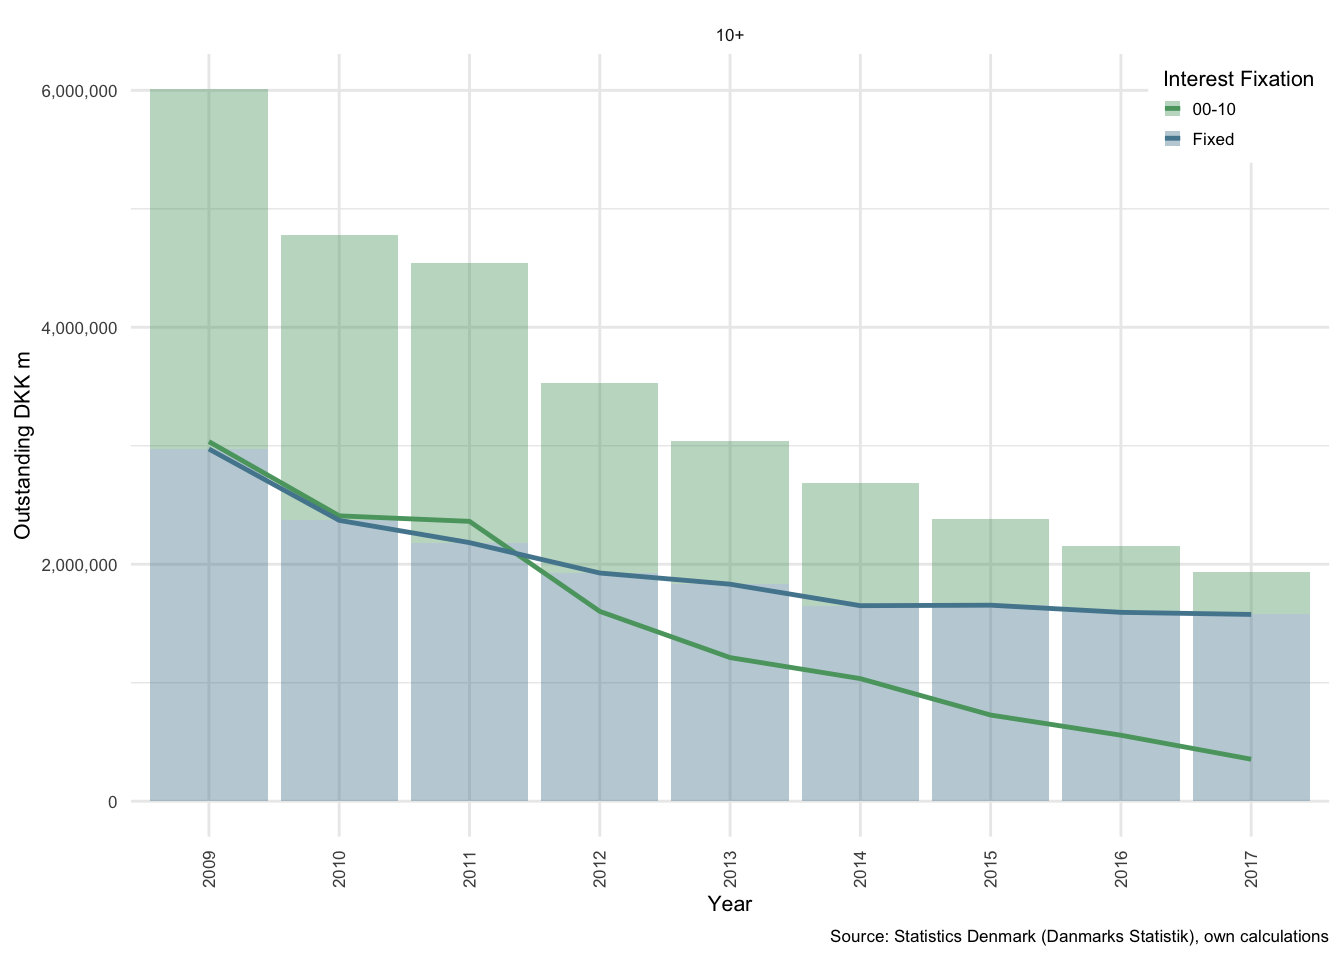
\includegraphics[width=0.95\linewidth]{figures/debt-composition-dk-simp-term-1-1} \caption{Interest payments}\label{fig:debt-composition-dk-simp-term-1}
\end{figure}

The cost of the outstanding debt has not followed the same pattern. Figure \ref{fig:debt-composition-dk-simp-term} part (b) above, shows that the total interest expenses paid on shorter ARM debt has declined in nominal terms from roughly equivalent to the fixed-interest debt in 2011 to just a fraction of total interest paid on fixed-interest products by the end of 2017.

This can then be represented as an average rate of interest by calculating the amount paid divided by the total outstanding debt. In Figure \ref{fig:interest-rate-composition-dk-simp}, the short-term-to-maturity characteristics are shown on the left to illustrate the these products follow market rates more closely. Again, however, it is the panel to the right that we are most interested in, where it is possible to see that longer term ARM debt paid an average rate of just under 0.5\%, while fixed rate longer term debt paid on average approximately 2.4\% in 2017. The spread has interestingly remained relatively constant between the two average rates, but the proportional decline in the ARM average rate has been approximately -86\%, while the same for fixed rate products has been approximately -50\%. It appears, from this illustration, that a fall in official interest rates has passed through to mortgage markets at roughly the same speed in fixed and ARM products\footnote{Although it is beyond the scope of this study, a useful experiment would be to estimate the total expected effect on household equity positions for an increase in interest rates, taking refinancing opportunities into account. Unfortunately data is not available to simply measure this impact directly, but it could be accomplished with reasonable assumptions. Measuring interest payments relative to debt in isolation unfortunately cannot capture this effect.}.

\begin{figure}
\centering
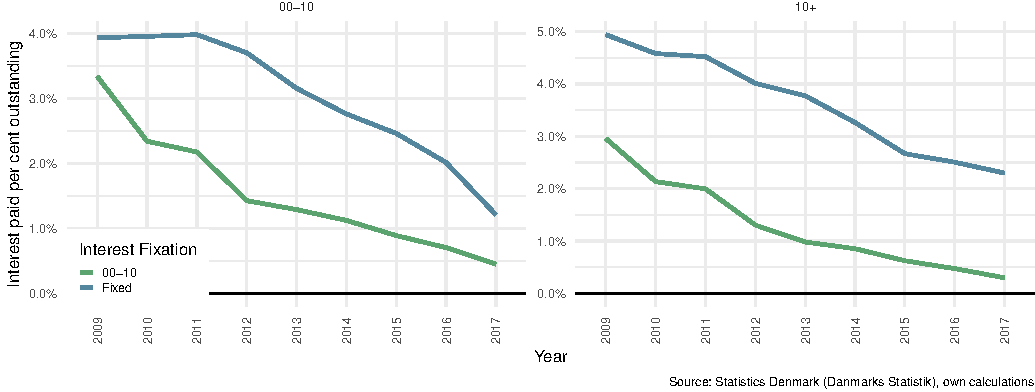
\includegraphics{figures/interest-rate-composition-dk-simp-1.pdf}
\caption{\label{fig:interest-rate-composition-dk-simp}Interest paid per cent of mortgage debt outstanding: By term}
\end{figure}

As can be expected, in the Danish environment, as interest rates fall and the option to refinance remains available to households, the rate of interest on fixed-interest securities has followed the flexible rate of interest downwards - with a relatively constant spread of approximately 2\% points. Unfortunately we do not have data on how this spread alters during a rising interest rate period. It can be seen that there was some delay in convergence in shorter terms to maturity. This is expected as the costs associated with refinancing existing contracts are likely to outweigh the benefits of a reduction in interest expense on smaller capital values, or on products with shorter terms to maturity (i.e.~fewer interest payments remaining).

In a rising rate environment borrowers again have the incentive to refinance in order to take advantage of falling bond prices, since in Denmark the borrower has the option to either pay back the cash capital value or to repurchase an equivalent bond to the one issued on the date of borrowing (otherwise known as a prepayment or buy-back option). If interest rates rise sufficiently to make it profitable, and if they have accumulated sufficient equity, the borrower has the opportunity to make a substantial reduction in the outstanding capital amount. Thus, unless rates remain unchanged, or only vary marginally, for an extended period of time, the proportion of outstanding debt that has been recently refinanced will typically be quite high\footnote{This is indeed the case at present, after interest rates declined gradually, but ultimately to a record low level in 2019. At the time of writing it is possible to borrow at a fixed rate for 30 years (the longest term to maturity available at present) of 0.5\% p.a. against 80\% of the market value of a primary residence. As can be seen from Figure \ref{fig:debt-values-dk-det-term} in the text above, approximately 85\% of mortgage debt outstanding has more than 25 years remaining to maturity. In other words, 85\% of all mortgage contracts in Denmark (by value) were issued inside of the previous 5 years.}.

\hypertarget{affordability-of-debt}{%
\subsubsection{Affordability of debt}\label{affordability-of-debt}}

The debt-service ratio (DSR) is shown in Figure \ref{fig:debt-service}, and calculated as the ratio between total outgoing property income payments to annual HH disposable income. In aggregate terms, it is unsurprising that the DSR has fallen continuously for the Danish household sector since the GFC. It is presently at the lowest level since 1995, and according to data collated by \citet{abildgren2017}, the lowest level ever. Thus in relative terms, while debt may be at record high levels relative to income, the aggregate cost of servicing that debt is at an all time low.

\begin{figure}[H]
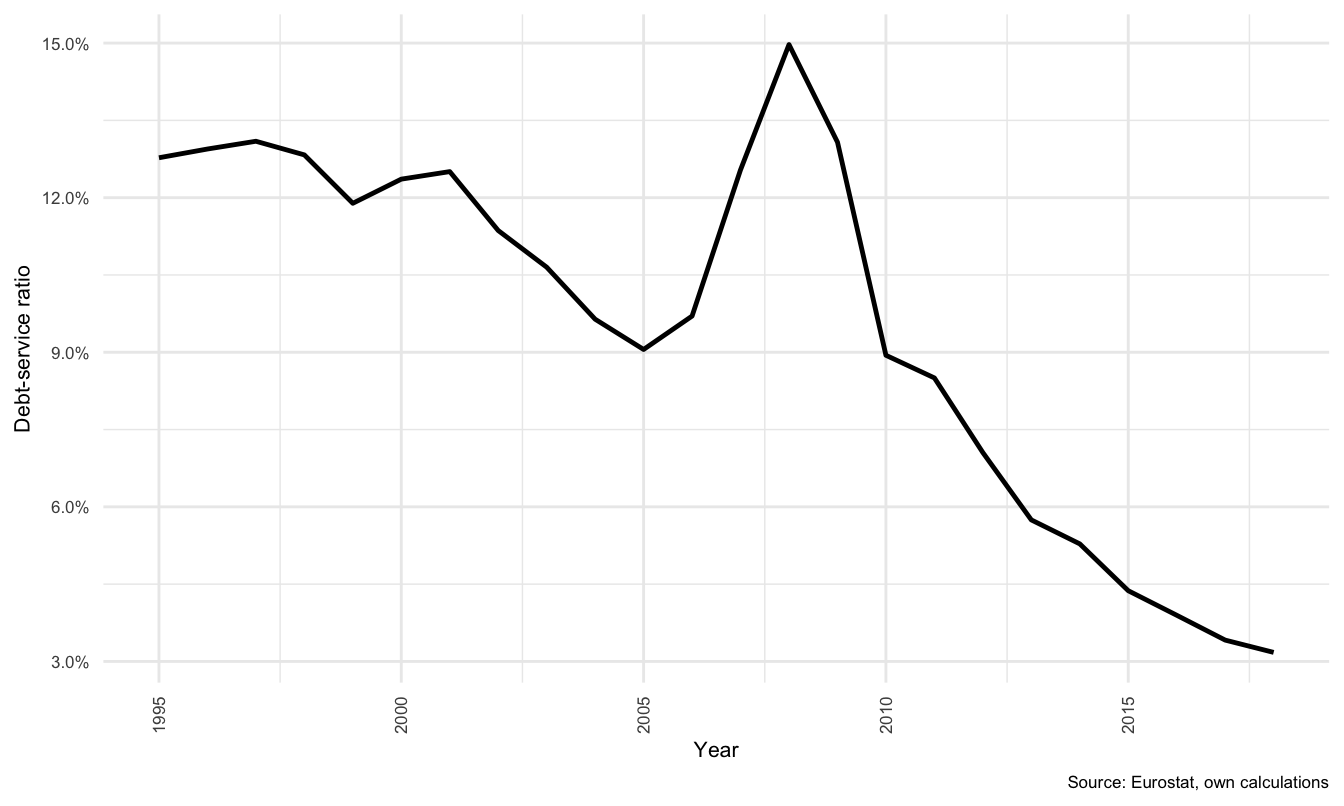
\includegraphics[width=0.6\linewidth]{figures/debt-service-1} \caption{Debt-service ratio: Denmark}\label{fig:debt-service}
\end{figure}

This paradox between the level of debt outstanding and the declining DSR
is discussed in analysis in Section \ref{sec:fi-fl-sfc-simulations} The implications for the
economy as a whole and for the household sector depend on the macroeconomic linkages
between the sectors and the drivers of agent decision-making in the model structure.

\hypertarget{sec:fi-fl-sfc-model-features}{%
\section{The model}\label{sec:fi-fl-sfc-model-features}}

The model implemented in this section is based on \citet{byrialsenraza2019empirical}, which is at the time of writing the most advanced empirical Stock-Flow-Consistent (SFC) macroeconomic model of Denmark. The full model together with an explanation for each equation and the logical connections between each of the sectors, flows and stocks is provided in Section \ref{sec:fi-fl-sfc-full-model}, in the appendix.

Throughout this section some of the equations and explanations thereof are duplicated for explanatory purposes. It will provide only a brief summary of the core features of the model, and the highlight the main changes made for this analysis.

The model consists of the five main institutional sectors, namely the household sector (HH) non-financial corporate sector (NFC), the financial corporate sector (FC), the general government (G), and the rest of the world (ROW). It was developed between 2017 and 2019 with a focus on the Danish HH. As such, the behaviours of all sectors are significantly simplified, except in so far as they engage directly with HH. The model is fully empirical, in the sense that all variables included in the model are available as a dataset, against which the performance of the model can be tested.

One feature is worth noting up front. As mentioned in the introduction, the full model has 131 endogenous and 78 exogenous variables. Included in the exogenous variables are all rates of return and all financial asset prices. The most important implication is that correlated asset price and market movements are not endogenous in the model, and this limits the analysis to very short-term model responses.

\hypertarget{data}{%
\subsection{Data}\label{data}}

The data used for the model in this article is sourced from a combination of Eurostat data, OECD data, and AMECO data. The period for which annual data is available in sufficient detail is from 1995 to 2017. This data is then processed in a series of aggregations. The data and the model accounting structures follow the ESA 2010 \citep{ESA2010} accounting structure, and the contents of the financial balance sheet can be summarised as:

Monetary gold and special drawing rights (F1), Currency and deposits (F2), Debt securities (F3), Loans (F4), Equity and investment fund shares (F5), Insurance, pensions and standardized guarantee schemes (F6), Financial derivatives and employees stock options (F7) and Other accounts (F8). These data are aggregated according to Table \ref{tab:eurostat-aggregation-table}.

\begin{table}

\caption{\label{tab:eurostat-aggregation-table}Aggregation of ESA balance sheet categories}
\centering
\fontsize{10}{12}\selectfont
\begin{tabular}[t]{l|l}
\hline
\multicolumn{1}{c|}{Assets} & \multicolumn{1}{c}{Eurostat Code (ESA 2010)} \\
\cline{1-1} \cline{2-2}
Interest bearing (\$IB\$) & \$F\_1\$, \$F\_2\$, \$F\_3\$, \$F\_4\$, \$F\_7\$ or \$F\_8\$\\
\hline
Net interest bearing (\$NIB\$) & \$F\_1\$, \$F\_2\$, \$F\_3\$, \$F\_4\$, \$F\_7\$ or \$F\_8\$\\
\hline
Net equities (\$NEQ\$) & \$F\_5\$\\
\hline
Pension (\$PEN\$) & \$F\_6\$\\
\hline
\end{tabular}
\end{table}

The financial markets are thus highly aggregated in the model with effectively only three asset classes. \(IB\) covers all securities that provide a financial return that is analogous to interest, as does \(NIB\). The only difference is that for NFC, GOV and ROW, as part of the aggregation process, only the net position in these assets and liabilities are considered.

The other two major asset classes are equities and pension funds. All except HH equities are expressed as net equity assets and liabilities, \(NEQ\), and for HH they are expressed as equity assets, \(EQA\), as they cannot issue equity liabilities by definition. Pension assets are expressed as \(PEN\), and are recorded as net pension assets (\(NPEN\)) for ROW.

\hypertarget{major-changes}{%
\subsection{Major changes}\label{major-changes}}

The most significant change in this version of the model is the introduction of a split between fixed and flexible rate mortgage debt. This relatively simple alteration allows one to test the sensitivity of HH balance sheets to a change in debt composition. The drivers of debt remain the same, and the rates of return on all other assets have been left unchanged.

This is to isolate the channel through which the change in the cost of borrowing affects households in the short term. This makes it possible to identify the transmission channels and magnitude of each shock more clearly. It is one of the advantages of fully exogenous rates of return and asset prices, but comes at the cost of more realistic inter-market (``pass-through'') responses.

\hypertarget{sec:fi-fl-sfc-model-tables}{%
\subsection{Balance sheet and transactions flow matrices}\label{sec:fi-fl-sfc-model-tables}}

As with all SFC models, the balance sheet matrix represents the distribution
of ownership of assets (\(+\)) and liabilities (\(-\)) in the modelled economy. As can be seen
from Table \ref{tab:sfc-fi-fl-BS}, the sum of all rows, with the exception of fixed capital, are zero. This reflects that each asset (except fixed assets, \(K\)) is exactly offset by a liability held by another sector.

The financial asset classes mentioned above are assigned to each sector according to assumptions of which sector issues or holds each type of security. FC holds the majority of counterpart financial securities, and in all sectors except HH, financial assets and liabilities are recorded in net terms (assets minus liabilities).

The interest bearing liabilities of HH are, as noted in the previous section, by a vast majority, long term debt. This is separated into fixed-interest (\(IBL(FI)^F\)) and flexible-interest (\(IBL(FL)^F\)) (or, ARM) mortgage liabilities.

Horizontal consistency captures the idea that all accounts are recorded as dual entry
accounting records, and the sum of all sector positions in any financial asset class should be zero. Vertical consistency represents the financial position of each sector, where financial net wealth (\(FNW\)) is the sum of all assets and liabilities and will either be a net positive or negative value. The sum across sectors of the \(FNW\) of all sectors is also zero.

\begin{table}

\caption{\label{tab:sfc-fi-fl-BS}Balance sheet matrix: BSM}
\centering
\fontsize{10}{12}\selectfont
\begin{tabular}[t]{l|c|c|c|c|c|c|c|c}
\hline
\multicolumn{1}{c|}{Stocks} & \multicolumn{1}{c|}{NFC} & \multicolumn{2}{c|}{FC} & \multicolumn{1}{c|}{GOV} & \multicolumn{2}{c|}{HH} & \multicolumn{1}{c|}{ROW} & \multicolumn{1}{c}{$Sigma$} \\
\cline{1-1} \cline{2-2} \cline{3-4} \cline{5-5} \cline{6-7} \cline{8-8} \cline{9-9}
\multicolumn{1}{c|}{ } & \multicolumn{1}{c|}{ } & \multicolumn{1}{c|}{Assets} & \multicolumn{1}{c|}{Liabilities} & \multicolumn{1}{c|}{ } & \multicolumn{1}{c|}{Assets} & \multicolumn{1}{c|}{Liabilities} & \multicolumn{1}{c|}{ } & \multicolumn{1}{c}{ } \\
\cline{3-3} \cline{4-4} \cline{6-6} \cline{7-7}
Interest bearing (IBA / IBL) &  &  & $-IBL^{F}$ &  & $+IBA^{H}$ &  &  & 0\\
\hline
\multicolumn{9}{l}{\textbf{Financial Stocks}}\\
\hline
\hspace{1em}Interest bearing Fixed &  & $+IBA(FI)^{F}$ &  &  &  & $-IBL(FI)^{H}$ &  & 0\\
\hline
\hspace{1em}Interest bearing Flexible &  & $+IBA(FL)^{F}$ &  &  &  & $-IBL(FL)^{H}$ &  & 0\\
\hline
\hspace{1em}Net interest bearing (NIB) & $NIB^{N}$ & $NIB^{F}$ &  & $NIB^{G}$ &  &  & $NIB^{W}$ & 0\\
\hline
\hspace{1em}Net equities (NEQ) & $NEQ^{N}$ & $NEQ^{F}$ &  &  & $NEQ^{H}$ &  & $NEQ^{W}$ & 0\\
\hline
\hspace{1em}Pensions (PEN) &  &  & $-PEN^{F}$ &  & $+PEN^{H}$ &  & $NPEN^{W}$ & 0\\
\hline
\midrule Financial net wealth (FNW) & $FNW^{N}$ & $FNW^{F}$ &  & $FNW^{G}$ & $FNW^{H}$ &  & $FNW^{W}$ & 0\\
\hline
\multicolumn{9}{l}{\textbf{Fixed Stocks}}\\
\hline
\hspace{1em}Fixed assets (K) & $K^{N}$ & $K^{F}$ &  & $K^{G}$ & $K^{H}$ &  &  & $K^{T}$\\
\hline
\end{tabular}
\end{table}

The transactions flow matrix is presented below. This matrix, much like the balance sheet matrix presented above, observes the requirements of horizontal and vertical consistency. In this table, all items that result in a positive flow of funds for the sector in question are marked with a plus sign (\(+\)), and all those that result in a flow outwards of funds are marked with a minus sign (\(-\)).

The expenditure approach to GDP is captured in the first five lines of the table, and can be captured as,

\begin{equation}
Y = C + I + G + (X - M)
\label{eq:gdp_intext}
\end{equation}

Where \(C\) is consumption, \(I\) is investment, \(G\) is government expenditure, \(X\) is exports and \(M\) is imports. All in nominal terms to reflect the actual flows of funds in each period. The income approach to national expenditure is captured in the following six lines in the table up until the row called \emph{Savings}. Each row name reflects the flow that is applicable to each sector. The full detail of how these flows are defined can be found in the full model description in Section \ref{sec:fi-fl-sfc-full-model}, in the appendix.

Capital income (\(rK\)), transfers (\(STR\)), capital transfers (\(KTR\)), acquisitions less disposal of fixed assets (\(NP\)) and net lending (\(NL\)) are presented without a particular sign attached to each sector. The reason for which is that each sector both receives and pays social transfers, and although GOV is the primary counterpart for all of these, the size and net sign of these transfers can change over time. The same is true for \(KTR\) and \(NP\). Net lending (\(NL\)) is a passive (residual) value and is determined by the balance of funding requirements between the sectors over time, and can therefore also swing between negative or positive as a flow.

\begin{table}

\caption{\label{tab:sfc-fi-fl-TFM}Transactions flow matrix: TFM}
\centering
\fontsize{10}{12}\selectfont
\begin{tabular}[t]{l|c|c|c|c|c|c|c|c|c|c|c}
\hline
\multicolumn{1}{c|}{Flows} & \multicolumn{2}{c|}{NFC} & \multicolumn{2}{c|}{FC} & \multicolumn{2}{c|}{GOV} & \multicolumn{2}{c|}{HH} & \multicolumn{2}{c|}{ROW} & \multicolumn{1}{c}{$Sigma$} \\
\cline{1-1} \cline{2-3} \cline{4-5} \cline{6-7} \cline{8-9} \cline{10-11} \cline{12-12}
\multicolumn{1}{c|}{ } & \multicolumn{1}{c|}{Current} & \multicolumn{1}{c|}{Capital} & \multicolumn{1}{c|}{Current} & \multicolumn{1}{c|}{Capital} & \multicolumn{1}{c|}{Current} & \multicolumn{1}{c|}{Capital} & \multicolumn{1}{c|}{Current} & \multicolumn{1}{c|}{Capital} & \multicolumn{1}{c|}{Current} & \multicolumn{1}{c|}{Capital} & \multicolumn{1}{c}{ } \\
\cline{2-2} \cline{3-3} \cline{4-4} \cline{5-5} \cline{6-6} \cline{7-7} \cline{8-8} \cline{9-9} \cline{10-10} \cline{11-11}
Private consumption & \$+C\$ &  &  &  &  &  & \$-C\$ &  &  &  & 0\\
\hline
Government consumption & \$+G\$ &  &  &  & \$-G\$ &  &  &  &  &  & 0\\
\hline
Investment & \$+I\$ & \$-I\textasciicircum{}\{N\}\$ &  & \$-I\textasciicircum{}\{F\}\$ &  & \$-I\textasciicircum{}\{G\}\$ &  & \$-I\textasciicircum{}\{H\}\$ &  &  & 0\\
\hline
Exports & \$+X\$ &  &  &  &  &  &  &  & \$-X\$ &  & 0\\
\hline
Imports & \$-M\$ &  &  &  &  &  &  &  & \$+M\$ &  & 0\\
\hline
\textbackslash{}midrule GDP & Y &  &  &  &  &  &  &  &  &  & 0\\
\hline
\textbackslash{}midrule Taxes & \$-T\textasciicircum{}\{N\}\$ &  & \$-T\textasciicircum{}\{F\}\$ &  & \$+T\textasciicircum{}\{G\}\$ &  & \$-T\textasciicircum{}\{H\}\$ &  & \$-T\textasciicircum{}\{W\}\$ &  & 0\\
\hline
Gross operating surplus & \$-B2\textasciicircum{}\{N\}\$ &  & \$+B2\textasciicircum{}\{F\}\$ &  & \$+B2\textasciicircum{}\{G\}\$ &  & \$+B2\textasciicircum{}\{H\}\$ &  &  &  & 0\\
\hline
Wages & \$-WB\textasciicircum{}\{N\}\$ &  &  &  &  &  & \$+WB\textasciicircum{}\{H\}\$ &  & \$WB\textasciicircum{}\{W\}\$ &  & 0\\
\hline
Capital income & \$rK\textasciicircum{}\{N\}\$ &  & \$rK\textasciicircum{}\{F\}\$ &  & \$rK\textasciicircum{}\{G\}\$ &  & \$rK\textasciicircum{}\{H\}\$ &  & \$rK\textasciicircum{}\{W\}\$ &  & 0\\
\hline
Transfers & \$STR\textasciicircum{}\{N\}\$ &  & \$STR\textasciicircum{}\{F\}\$ &  & \$STR\textasciicircum{}\{G\}\$ &  & \$STR\textasciicircum{}\{H\}\$ &  & \$STR\textasciicircum{}\{W\}\$ &  & 0\\
\hline
Pension adjustments &  &  & \$-CPEN\textasciicircum{}\{F\}\$ &  &  &  & \$+CPEN\textasciicircum{}\{F\}\$ &  &  &  & 0\\
\hline
\textbackslash{}midrule Savings (per sector) & \$-S\{N\}\$ & \$+S\{N\}\$ & \$-S\{F\}\$ & \$+S\{F\}\$ & \$-S\{G\}\$ & \$+S\{G\}\$ & \$-S\{H\}\$ & \$+S\{H\}\$ & \$-S\{W\}\$ & \$+S\{W\}\$ & 0\\
\hline
\textbackslash{}midrule Capital transfers &  & \$KTR\textasciicircum{}\{N\}\$ &  & \$KTR\textasciicircum{}\{F\}\$ &  & \$KTR\textasciicircum{}\{G\}\$ &  & \$KTR\textasciicircum{}\{H\}\$ &  & \$KTR\textasciicircum{}\{W\}\$ & 0\\
\hline
Acquisitions less disposal FA &  & \$NP\textasciicircum{}\{N\}\$ &  & \$NP\textasciicircum{}\{F\}\$ &  & \$NP\textasciicircum{}\{G\}\$ &  & \$NP\textasciicircum{}\{H\}\$ &  & \$NP\textasciicircum{}\{W\}\$ & 0\\
\hline
Net lending &  & \$NL\textasciicircum{}\{N\}\$ &  & \$NL\textasciicircum{}\{F\}\$ &  & \$NL\textasciicircum{}\{G\}\$ &  & \$NL\textasciicircum{}\{H\}\$ &  & \$NL\textasciicircum{}\{W\}\$ & 0\\
\hline
\textbackslash{}midrule \$\textbackslash{}Sigma\$ & 0 & 0 & 0 & 0 & 0 & 0 & 0 & 0 & 0 & 0 & 0\\
\hline
\end{tabular}
\end{table}

The three rows after the \emph{Savings} row illustrate adjustments to the level of savings (\(S\)) as a result of capital transfers (\(KTR\)), purchase and sale of fixed assets (\(NP\)) and (from the third row of the table) the level of investment (\(I\)) of each sector - summed vertically in the \emph{capital} accounts column for each sector. The sum of all of these items is reflected in a net financing requirement for each sector, in the table is called \emph{Net lending}. The sum of all net lending positions in the economy is again necessarily equal to zero, as one sector's surplus is at least one other sector's deficit. The sum of all columns and all rows are thus all equal to zero, and this criterion is respected by the data collected from Eurostat on an annual basis.

Financial and fixed assets in the model are subject to both transactions and revaluations (or capital gains or losses). The accumulation of certain types of assets or liabilities depends in part on the action of the sector in question and in part on the effects of the other sectors. As can be read in the full model description in the appendix, the nominal values that are sourced from the Eurostat database and or AMECO can then be deflated using appropriate price indices. There are 19 different price indices used in the model, some of which are calculated, but the majority of which are sourced either from Statistics Denmark, AMECO or the OECD. The details of the model structure and the performance of the model relative to the data available can be found in \citet{byrialsenraza2019empirical}, and the details of the behavioural equations available in Section \ref{sec:fi-fl-sfc-full-model}, in the appendix.

What we are most interested in here, however, is the specific channels through which the scenarios proposed below transmit. As mentioned above, the model contains active behaviours and passive behaviours. In each period, in order to ensure closure in the model, there is one variable in each sector that is passive to the budget constraints of each year.

The passive accumulator flows (or residual, buffer variables) for each sector are as follows:
transactions in net interest bearing securities for NFC (\(NIBTR^N_t\)), GOV (\(NIBTR^G_t\)), and ROW (\(NIBTR^W_t\));and, transactions in interest bearing assets for HH (\(IBATR^H_t\)).
While specific behavioural equations determine the holding of all other financial assets, \(NIB\) securities act as a catch all category for NFC, GOV and ROW. The sum of those positions is then absorbed by FC. As will be discussed below, the final closure of the model is provided through the indirect provision of equity assets to HH by FC on demand. This is fitting, since HH purchases of mutual funds or unit trusts are likely to be fulfilled by FC, rather than directly by NFC.

\hypertarget{sec:fi-fl-sfc-scenarios}{%
\section{Scenarios}\label{sec:fi-fl-sfc-scenarios}}

This section briefly explains the four scenarios investigated using the model. Apart from alterations to the structure of household mortgage liabilities, the model operates in the same manner as in \citet{byrialsenraza2019empirical}. The shocks presented below are measured as a percentage change from the baseline scenario.
This allows for a simpler comparison between scenarios, and the aggregate nominal
and real values of stocks and flows are illustrated where relevant.

The first shock (and Scenario 1) is an increase in interest rates in 2020, the second shock (and Scenario 2) is a decline in property prices in 2022. Scenario 3 compounds the first two, in that the first shock is kept in the model before the shock to property prices is imposed. The last scenario, Scenario 4, is a reduction in the level of ARMs in 2017. Effectively, the last scenario changes the pre-conditions for the first two shocks, but applies them in exactly the same manner. It is therefore possible to make a direct comparison between Scenario 3 and Scenario 4, given two different starting points.

This ordering allows the answer to a counter-factual question: What if HH had not taken on as much flexible rate mortgage debt? How would this shift in interest rate exposure affect outcomes, both for HH and the broader economy? In essence, what might have been the case if the innovations leading up to 2003 had not impacted borrowing decisions to the same degree? There are however, some limitations to the current model that are relevant for this exercise.

\hypertarget{sec:fi-fl-sfc-scenarios-limitations}{%
\subsection{Limitations for interpretation of results}\label{sec:fi-fl-sfc-scenarios-limitations}}

\emph{Adjustable Rate Mortgages (ARMs) typically do not adjust immediately}

As noted above, the bulk of ARMs in Denmark adjust fewer than 5 years into the future. This allows households an extended period of time to observe interest rate fluctuations and make a decision regarding refinancing or property sale. It also means that the effects of an interest rate change will only impact HH cash flows after between one and five years.

\emph{A decline in house prices is unlikely to happen in isolation}

A fall in house prices is not expected to occur in isolation. Unlike in the model below, a collapse in property prices is unlikely to be an isolated event. It would more likely accompany broader systemic problems or be triggered by some form of financial or economic crisis.

\emph{The structure of the economy at end 2017 is integrated with the volume and structure of household debt}

For the fourth scenario, it is assumed that we can simply shift the structure of debt and leave the remainder of the economy unchanged. In reality, the total level of debt outstanding would probably be significantly lower if ARM and interest-only products had not been made available. This would have affected a significant array of economic variables, not least of all, domestic demand and house prices. Although this is true, HH have already accumulated significant levels of debt. As such, Scenario 4 is less a question of, what if things had been different, and more a question of how to structure policy in order to best influence future refinancing decisions of HH.

\emph{Interest rate changes would change the composition of debt}

Refinancing in response to interest rate changes in Denmark is extensive. In a rising interest rate environment, the incentive is to repurchase the previously issued bond at a reduced price, settle the older debt, and then refinance at similar monthly instalments, but with a lower capital value outstanding.

With falling interest rates, the incentive is to refinance at lower monthly instalments, and if possible using a bond with fixed-interest, thus creating the opportunity to refinance if rates rise significantly in the future, and thus reduce the level of debt outstanding. It is therefore unlikely that the structure of debt would remain constant after a shift in rates\footnote{Micro-level contractual data is presently only available from 2009 onwards, thus at an individual level, there is no data that can be used to model household behaviour in response to an increase in interest rates. If the home owner intends to sell their property inside of 5 years, interest rates must fall dramatically for it to be financially beneficial to refinance due to the costs involved. In a rising interest rate environment, a fixed-interest bond holder that sells their property will always be able to benefit from capital losses on their outstanding bond, but might face difficulties in selling their property as demand is expected to be suppressed due to higher borrowing costs. In the same situation, a fixed rate borrower will again need quite significant changes in the level of interest rates for a prepayment or buy-back operation to be profitable in under 5 years.}. Due to the costs involved in refinancing, a change in interest rates is expected impact debt structures gradually, remaining fairly stable for the first year or two, and adjusting to a greater degree in the medium term (approximately up to 5 years).

\hypertarget{sec:fi-fl-sfc-scenarios-s1}{%
\subsection{Scenario 1 - An increase in interest rates}\label{sec:fi-fl-sfc-scenarios-s1}}

The first shock is a simple interest rate change. The point is to illustrate the expected impact on the level of household disposable income and the household balance sheet.

In this shock we consider a 2 percentage point (\(2\%\) points) rise in official rates. This is assumed to be passed through perfectly to ARM mortgages (interest rate on flexible-interest-rate mortgage debt, i.e.~flexible rate products, with subscript (FL), (\(r^H_{L(FL)_{t}}\)). The cost of fixed-interest mortgage debt (\(r^H_{L(FI)_{t}}\)) is increased by a proportionally lower adjustment of point five percentage points (\(0.5\%\) points) to reflect lower sensitivity of adjustments of the overall stock of fixedinterest rate products. This is a strong assumption, and is not likely to hold over longer periods of time, fixed-interest rate debt holders are expected to retain their debt at lower interest rates, while the majority of flexible-interest rate holders are expected to participate fully in the rise in interest rates after a period of three years\footnote{These time periods are purely for illustrative purposes, since, as mentioned just above, the Danish market is expected to have extensive refinancing as rates shift. This is however expected to be somewhat muted by the expectation that the demand for new debt, and therefore the demand for houses are expected to fall - potentially leading to a fall in house prices, or at the very least, slower capital gains. Selling conditions are generally expected to be worse in a higher interest rate environment, where the rise in the cost of house purchase will naturally exclude a large number of potential buyers.}.

In the model baseline, the current rate is calculated as interest payments relative to outstanding debts. This gives a weighted average at the end of 2017 of 1.41\% for all debts\footnote{As noted earlier, interest rates are currently at historically low levels. The actual average rates of interest paid on flexible and fixed-interest mortgage products were 0.29\% and 2.29\% per annum at the close of 2017. These values, however exclude a variety of debt types such as bank debt, vehicle finance and consumer credit. The use of the average payment on all debt types is a simplification that is made to suit the aggregation of data, and the reader should be aware that this does not take into account the multitude of behavioural incentives that apply to each underlying debt type.}. After the shock, the adjustment is from this average rate upwards - thus flexible-interest rates are adjusted up to 2.41\% and fixed-interest rates up to 1.91\%. This constitutes a 141.75 per cent increase in flexible rates, and taking into account changes in the level of outstanding debt in 2021, a 136.29\% increase in interest payments. For fixed-interest debt, it constitutes a 35.44 per cent increase in fixed rates, and a 32.38\% increase in interest payments.

The interest rates in the model include, interest on fixed (\(r^H_{L(FI)}\)) and flexible rate (\(r^H_{L(FL)}\)) mortgages, and the counterpart assets (\(r^F_{A(FI)}\), \(r^F_{A(FL)}\)), the general rate of return on net interest bearing assets (\(r_{N}\)), and the return on interest bearing assets for households (\(r^H_{A}\)). The other rates of return are the domestic and foreign rate of return on equities (\(\chi _t\)), and pension assets (\(\psi _t\)). All rates of return in the model are determined exogenously, which means that any adjustment must be applied manually. As noted above, the change is limited to the cost of borrowing for HH only.

In the case of household debt, it is FC that holds the counter-balance assets. Thus,

\[r^F_{A(FI)_{t}} = r^H_{L(FI)_{t}}\]
and,
\[r^F_{A(FL)_{t}} = r^H_{L(FL)_{t}}\]

FC receives \(r^F_{A(FI)_{t-1}}(IBA^{F\sim H}_{A(FI)_{t-1}})\), and the two interest rates are simply made equivalent. An increase in rates results in an increase in costs for HH and an increase in revenues for FC.

Figure \ref{fig:dst-mortgage-debt-interest} illustrates, in part (a) the actual monthly interest rates available for new debt on Danish mortgage markets since 2013 (separated by term of interest fixation). Part (b) shows the progression of official interest rates in Denmark since 2000, where the ``Mortgage bond'' rate is the dark-red line, and is comparable with \emph{Fixed} mortgage bonds in panel (a), the purple line, from 2013 onwards. Part (c) illustrates the impact of the shock to interest rates in the model in 2020.

\begin{figure}[H]
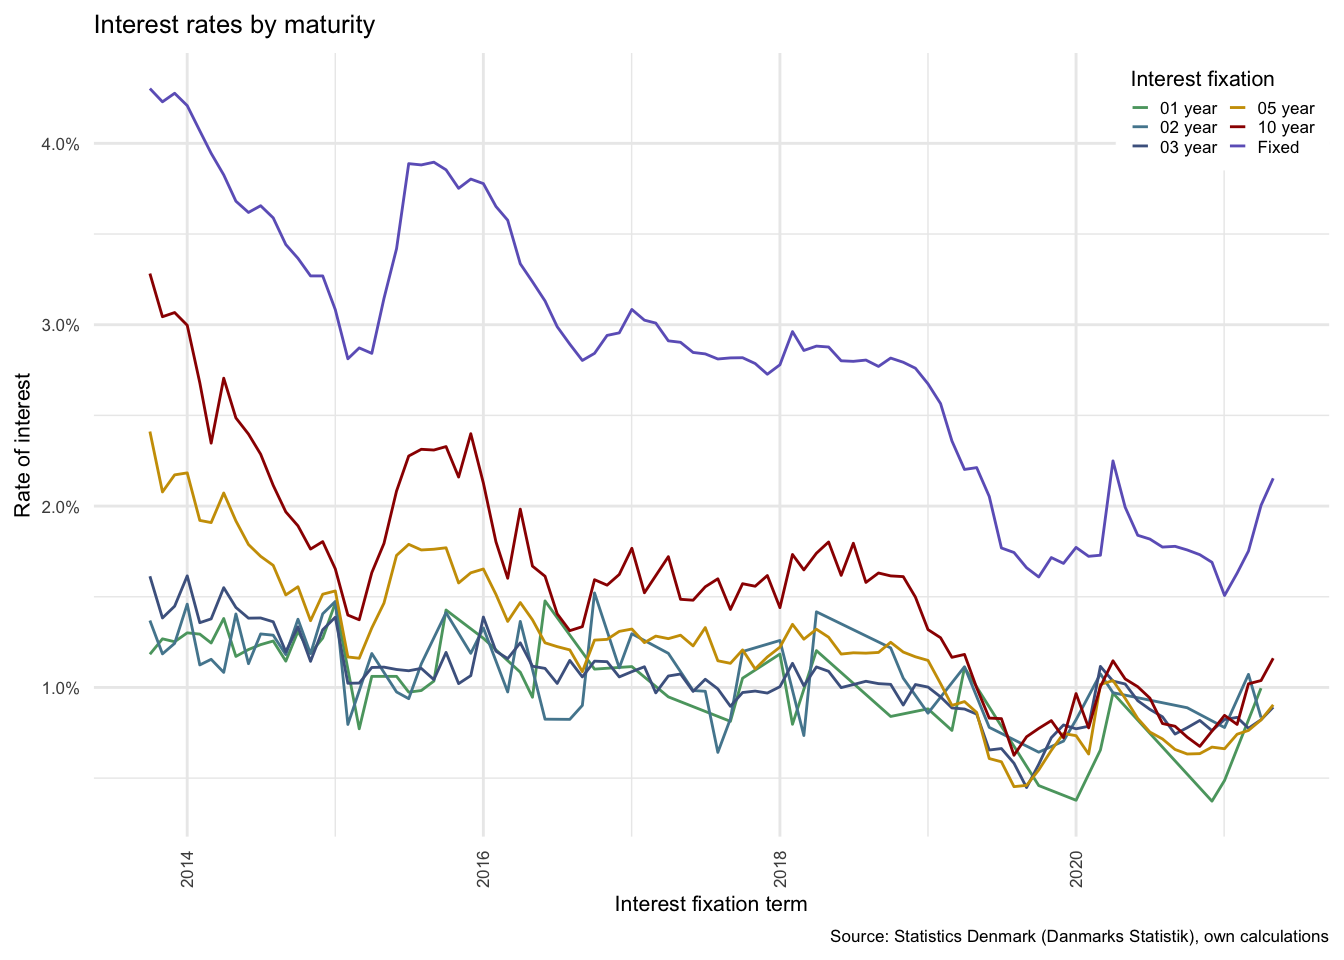
\includegraphics[width=0.33\linewidth]{figures/dst-mortgage-debt-interest-1} 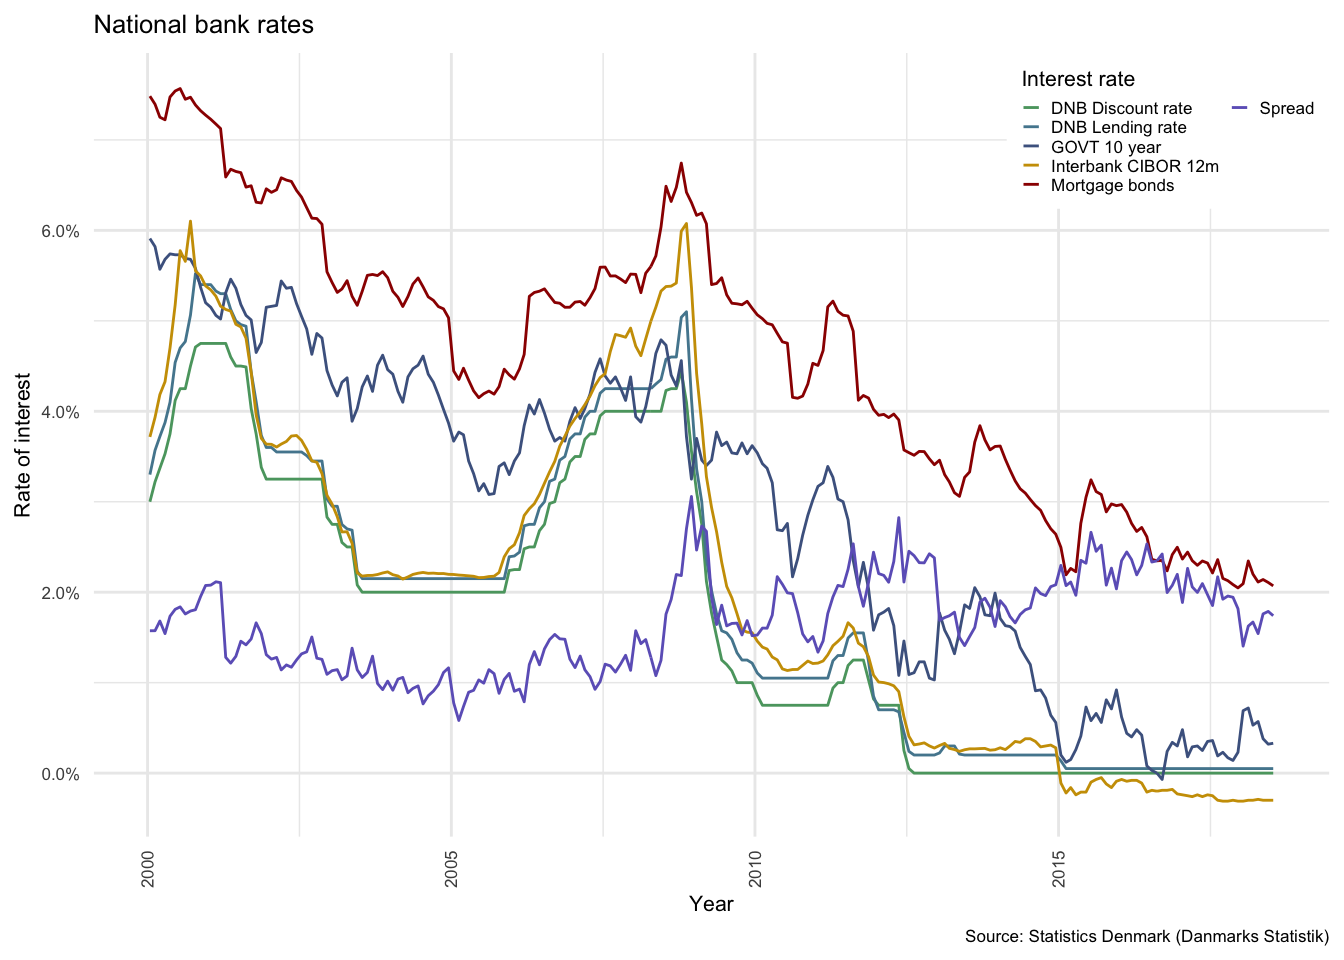
\includegraphics[width=0.33\linewidth]{figures/dst-mortgage-debt-interest-2} 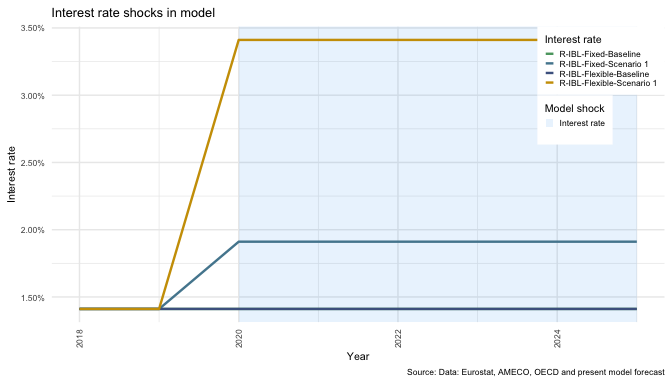
\includegraphics[width=0.33\linewidth]{figures/dst-mortgage-debt-interest-3} \caption{Interest rates in Denmark}\label{fig:dst-mortgage-debt-interest}
\end{figure}

As can be seen from part (a), the rates available to fixed rate borrowers have followed market rates downwards throughout the period, although this illustrates only those rates available, rather than those paid. Figure \ref{fig:interest-rate-composition-dk-simp} showing the amounts actually paid in the section above, however, illustrates that the amount paid has also declined at a similar pace, although with a marginal delay.

The interest rates in the model are split into fixed and flexible rates for the purpose of
testing the effects of a shock to interest rate on alternative compositions of mortgage debt.
The baseline value of interest rates remains just below 1.5\% on average for all debt.

The expected outcome is that where the proportion of fixed-interest outstanding debt is higher, the effects of a shock will be weaker, and vice versa. This of course can only have an impact in the case where mortgage debt is itself split into fixed- and flexible-rate debt.

The total level of outstanding \(IBL\) for HH is split into fixed-interest (\(IBL_{FI}\)) and flexible-interest bearing liabilities (\(IBL_{FL}\)). The proportion of interest bearing assets held as \(IBL_{FI}\) is \(\alpha\).

\begin{equation}
IBL^H_{{FI}_t} = \alpha(IBL^H_t)
\end{equation}

and thus,

\begin{equation}
IBL^H_{{FL}_t} = (1-\alpha)(IBL^H_t)
\end{equation}

The level of \(\alpha\) is calculated from data acquired from multiple data sources at Statistics Denmark, and varies over time. The split was first introduced in 1996, but initial volumes were low. As discussed in Section \ref{sec:fi-fl-rk-dk}, while the composition of this debt is significantly more complex than this, a strong argument can be made for an aggregation up to just these two categories. This split has no effect on the model prior to the shock in 2020, as the rate of interest on each is considered to be equal to the average rate used in the baseline scenario up to that point.

It is also possible to shock all other rates of return to a similar degree. Given the integration of financial markets, this would produce results in the model that are more realistic. Unfortunately, it would also conceal the effects that are purely due to dynamics linked to the interest cost of borrowing for households\footnote{Several alternative formulations of the shock were tested, but the inclusion of changes to other rates of return require a number of additional assumptions. For example, an increase in domestic bond rates are only likely in Denmark if European interest rates also rise. Also, the speed and proportion to which rates pass through from official rates to each market are likely to differ across products, but also over time.}.

\hypertarget{sec:fi-fl-sfc-scenarios-s2}{%
\subsection{Scenario 2 - A fall in house prices}\label{sec:fi-fl-sfc-scenarios-s2}}

The second scenario is a fall in house prices. This is effected through a negative twenty per cent adjustment to the house price index (\(-20\%\)). This is a large change to house prices, but is equivalent to the stress test applied by the IMF \citep{sheehy2014}. At a national level, Figure \ref{fig:fl-fi-house-prices-national} illustrates that the average nominal house price index (HPI) for dwellings in Denmark has risen at a relatively steady pace since the GFC.

\begin{figure}[H]
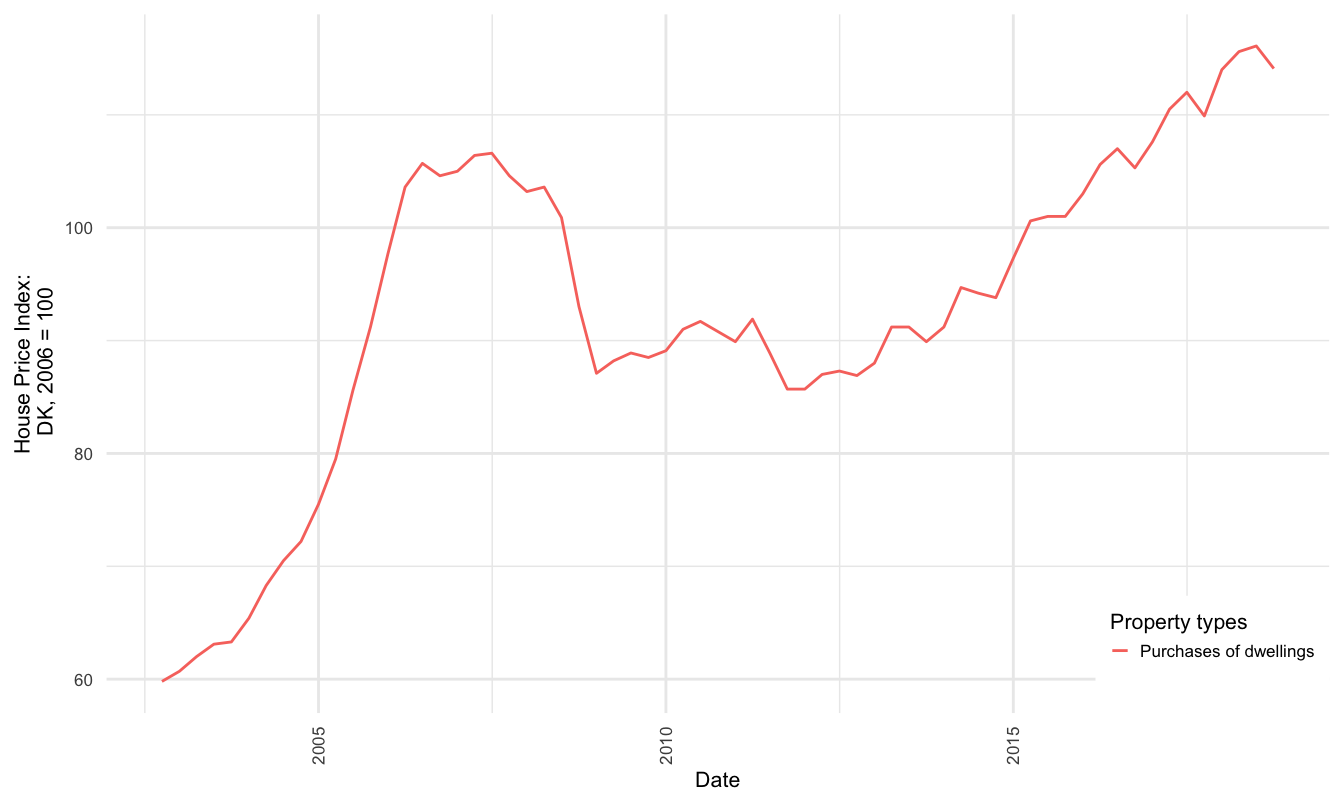
\includegraphics[width=0.7\linewidth]{figures/fl-fi-house-prices-national-1} \caption{National House price index (HPI), 2006 = 100}\label{fig:fl-fi-house-prices-national}
\end{figure}

This follows a collapse of house prices during the GFC, where prices of Danish dwellings fell approximately 20\% from the peak in 2006 to the trough in 2011. This average was not uniform across property types or regions. As shown in Figure \ref{fig:fl-fi-house-prices-regional}, the prices of owner occupied flats in the Capital and North Denmark Regions have risen at roughly the same pace as prior to the GFC. This is not predictive of a correction or price collapse, but does suggest a possible housing price bubble in those markets. All other regions, appear to have only just recovered to pre-crisis prices\footnote{The capital region holds a disproportionately large share of real estate assets by value, and thus the impact of property prices there carry a greater weight for an average for the country as a whole.}.

\begin{figure}[H]
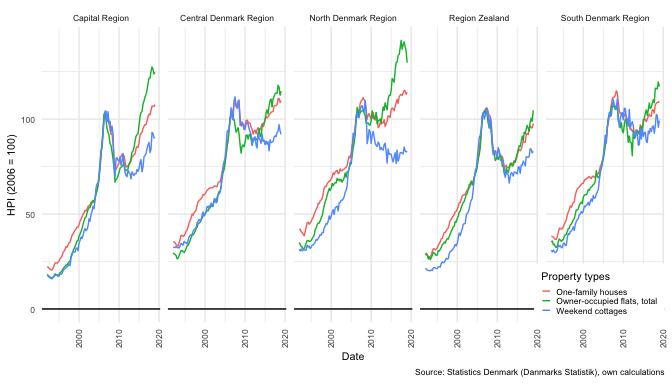
\includegraphics[width=0.95\linewidth]{figures/fl-fi-house-prices-regional-1} \caption{House price index (HPI), 2006 = 100}\label{fig:fl-fi-house-prices-regional}
\end{figure}

A more serious concern for potential borrowers is that several markets, particularly those for weekend cottages (otherwise known as summer houses) have not recovered in the period following the GFC. Thus, any property purchased between 2005 and the collapse in 2007 would have a high probability of falling into negative equity\footnote{Although the risk that the LTV ratio rises above 1 is lower for cottages, since the cap on bond financing has until very recently been significantly lower than for primary residences (60\% as opposed to 80\%).}.

In this model, households are only permitted to make productive investment in
housing, which, as in \citet{Zezza2008}, \citet{fontana2013securitization} and \citet{beckta2015modelling}, is considered only as a primary market. The major difference here is that households are assumed to produce the houses, whereas firms are housing producers for all three of the above-mentioned studies. The secondary market for houses is assumed to affect prices, but not the demand for additional housing investment. Demand for housing investment is determined by by a Tobin's-Q-like function, partially driven by changes in disposable income and previous period housing investment, and partially driven by a relative shift in sales price (\({P^H_{t-i}}\)) and construction cost (\({P^i_{t-i}}\)) indices.

Real investment in fixed assets (dwellings), in Equation \ref{eq:realhousinginvestment_intext}, is estimated as a log-linear function that depends on conditions in previous periods. This assumes that the decision to invest in houses occurs based on recent developments, but that actual changes in investment in fixed assets takes some time to materialise. It thus takes one period before the effects of the house price shock can be observed.

\begin{equation}
ln(i^H_t) = \beta _i + \beta _i ln(i^H_{t-i}) + \beta _i ln \Bigg( \frac{P^H_{t-i}}{P^i_{t-i}}\Bigg) + \beta _iln(yd^H_{t-i})
\label{eq:realhousinginvestment_intext}
\end{equation}

The shock imposed on the model is to the numerator of the Tobin's Q ratio\footnote{In the present structure of the model, investment is regressed against real investment of the previous period \(i^H_{t-1}\); real disposable income \(y^H_{d}\), and the same at \(t-2\) (\(y^H_{d_{t-2}}\)); the Tobin's Q ratio at level terms \(\Bigg( \frac{P^H_{t}}{P^i_{t}}\Bigg)\), and with a one period lag \(\Bigg( \frac{P^H_{t-1}}{P^i_{t-1}}\Bigg)\); a constant; and, a trend component.}. The imposed decline in house prices affects sales prices negatively, relative to the cost of production, and thus has a contractionary effect on the Tobin's q ratio, \(\Bigg(\frac{P^H_{t-i}}{P^i_{t-i}}\Bigg)\), and thus on HH real investment (\(i^H_t\)). The shock is implemented as a permanent decline in prices, and thus changes the value of the ratio for all periods following the shock. Growth in house prices continues according to the same trajectory as in the baseline in order to make for a more effective comparison.

The nominal level of investment in housing can be calculated by inflating the real investment in housing
series (\(i^H_t\)) by the investment price index (\(P^i_t\), which is sourced from Statistics Denmark):

\begin{equation}
I^H_t = i^H_t(P^i_t)
\end{equation}

The nominal stock of housing (\(K^H\)), as with other assets to come, follows the simple
process of previous stock (\(K^H_{t-1}\)), plus acquisition (in this case investment in new houses), less depreciation (\(D^H_t\)) plus capital gains (\(K^H_{CG_t}\)).

\begin{equation}
K^H_t = K^H_{t-1} + I^H_t - D^H_t + K^H_{CG_t}
\label{eq:nominalhoushingcapital1}
\end{equation}

Capital gains on houses, in turn, can be calculated in an \emph{ex post} manner as:
\begin{equation}
K^H_{CG} = \Delta P^H_t (K^H_{t-1})
\end{equation}

Which is simply the change in the price of houses applied to the level of stock at
the end of the preceding period.

The change in house prices (\(\Delta P^H_t\)) leading into the current period is then by definition the same ratio proportion of capital gains to previous housing capital.

\begin{equation}
\Delta P^H_t = \frac{KH_{CG}}{K^H_{t-1}}
\label{eq:changehouseprice_intext}
\end{equation}

Nominal housing capital held by HH at the end of the current period
can be expressed as the price adjusted stock at the end of the previous
period, plus net investment and depreciation. Equation \ref{eq:nominalhoushingcapital2}
is effectively a restatement of Equation \ref{eq:nominalhoushingcapital1}, but
with greater emphasis on the variable shocked in the analysis.

\begin{equation}
K^H_t = K^H_{t-1}(1 + \Delta P^H_t) + I^H_t- D^H_t
\label{eq:nominalhoushingcapital2}
\end{equation}

The deflated real capital index can then be found, as in Equation (\ref{eq:realhoushingcapital_intext}) by dividing the series by the investment (housing) price index, from Equation (\ref{eq:changehouseprice_intext}).

\begin{equation}
k^H_t = \frac{K^H_t}{P^i_t}
\label{eq:realhoushingcapital_intext}
\end{equation}

Housing capital then forms part of HH net wealth, which feeds back into consumption decisions in subsequent periods. A decline in net wealth in period \(t\) leads to a decline in consumption in period \(t+1\).

The effects of changes in net wealth (\(NW\)), are then felt directly in the level of HH consumption, but with a lag on one period (as can be seen in Equation (\ref{eq:hh_consumption}) in the appendix). Although a fall in house prices does not affect household disposable income to a substantial degree is contributes to a decline in overall economic activity, and therefore reduces the demand for labour in subsequent periods. This ultimately does affect household income but the effect is not as immediate as was the case for the interest-rate shock.

\hypertarget{sec:fi-fl-sfc-scenarios-s3}{%
\subsection{Scenario 3 - Combination of Scenarios 1 and 2}\label{sec:fi-fl-sfc-scenarios-s3}}

The third scenario consecutively applies the shocks from Scenarios 1 and 2. First the interest rate increase in 2020, and then the decline in property prices in 2022. This combination sets up the comparison to be introduced in Scenario 4 below.

\hypertarget{sec:fi-fl-sfc-scenarios-s4}\label{sec:fi-fl-sfc-scenarios-s4}}

The final alteration to the model is an increase in the proportion of mortgage debt held as fixed debt (\(\alpha\)) from the 2016 level of 33.42\% up to 80\% in 2017. This shift allows us to test the hypothetical difference of the impact of a shock to interest rates in an artificial scenario, where the proportion of flexible debt amounts to only 20\% of outstanding household mortgage liabilities.

\hypertarget{sec:fi-fl-sfc-simulations}{%
\section{Simulations}\label{sec:fi-fl-sfc-simulations}}

This section explains the transmission of the two shocks in the scenarios described above. First, the components of the economy that are most dramatically affected are identified, and thereafter the key transmission channels that cause these effects are briefly discussed.

The key take-aways from this section are that shock 1 and 2 both propagate through the economy as described above, and that Scenario 3 results in greater volatility in the responses of the economy than Scenario 4. This has implications for the stability of the balance sheets of each sector and for the economy as a whole.

The effects of each shock are summarised in tables in Section \ref{sec:fi-fl-sfc-Ap-A-scenario-summaries} for each of the above-mentioned scenarios\footnote{Those tables are organised, firstly, according to whether the affected variable is a stock, flow, parameter, rate, or index of some kind; and secondly, in order of largest variation from the baseline scenario (as a proportion of the baseline). Transactions in and revaluations in stocks, which occur on an annual basis, are considered flow variables. To capture accumulation effects, tables are provided at the end of period 2021 (\(t+1\)) for Scenarios 1 and at the end of periods 2022 (\(t\)) and 2025 (\(t+3\)) for Scenarios 2, 3 and 4.}. This approach allows a quick summary of the impacts of a shock. It shows all affected variables, and thus provides a snapshot of how broadly the shock propagates. One drawback is that it is a cross section in time, and thus is not able to show the progression of feedback effects over time. These tables are both used as a guide to the most important transmissions, and as a consistency check, to ensure that the model behaves within reason.

The model responds largely as expected to the first shock, with the exception of the rather extreme response of the financial sector. This is because FC transactions in net interest bearing assets (\(NIBTR^F\)) absorbs all financial transactions of the other sectors - or, stated differently, accumulates all financial imbalances. The second shock, to property prices, has a more interesting result with regard HH savings and will be discussed in more detail in the HH section below.

As noted above, each of the sectors has a buffer flow that summarises the collective effect of each shock, and each of the shocks are quite extreme in nature. It is therefore unsurprising that the effect on the passive elements is somewhat exaggerated. Even though shocks of the same magnitude have occurred in the past, they are not common events and have only been used here to enhance the potential risks associated with the different debt structures.

\hypertarget{general-economy}{%
\subsection{General economy}\label{general-economy}}

The first shock (to interest rates) has a delayed effect that is first visible in the shift from period 2020 to period 2021; as can be seen for Scenarios 1, 3 and 4. The second shock (to property prices) takes effect immediately in 2022, and can therefore be seen to take effect from period 2021 to period 2022 for Scenarios 2, 3 and 4. At a broader economic level, the strongest impact on the major components of GDP from the first shock are a decline in gross fixed capital formation (\(I\)) of -1.25\% and in imports (\(M\)) of -1.22\% (and as a result, net exports rise by just over 10.52\%). Figure \ref{fig:fl-fi-sfc-plot-gdp-indicators_s1_s2} shows how \(C\), \(I\), \(G\), \(X\) and \(M\) would evolve relative to the baseline, for scenarios 1 and 2, and Figure \ref{fig:fl-fi-sfc-plot-gdp-indicators_s3_s4} that shows the same for Scenarios 3 and 4.

The shock to interest rates only impacts the model at \(t+1\) and so there is no change from the baseline in year 2020, whereas the impact of a property price shock takes immediate effect in 2022. Exports remain relatively unchanged under both shocks, only marginally affected due to a shift in domestic prices. \(Y\), or GDP, is more affected by the shock to interest rates in Scenario 1 than by property prices in Scenario 2, largely as a result of the limited impact of the property price shock on \(C\) and \(M\). The rapid rise in interest costs clearly result in a decline in all demand components except for \(G\), which is exogenous and therefore remains completely unchanged in all scenarios.

\begin{figure}[H]
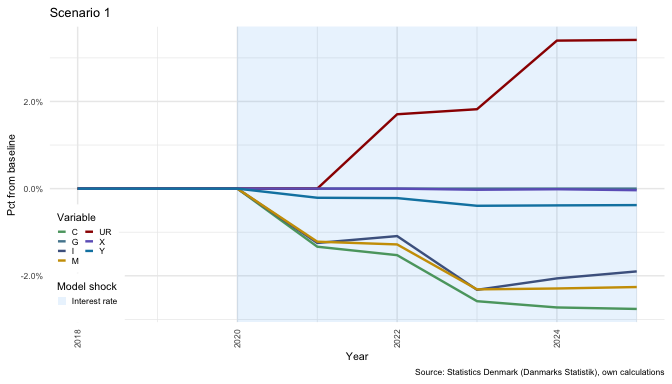
\includegraphics[width=0.5\linewidth]{figures/fl-fi-sfc-plot-gdp-indicators-s1-s2-1} 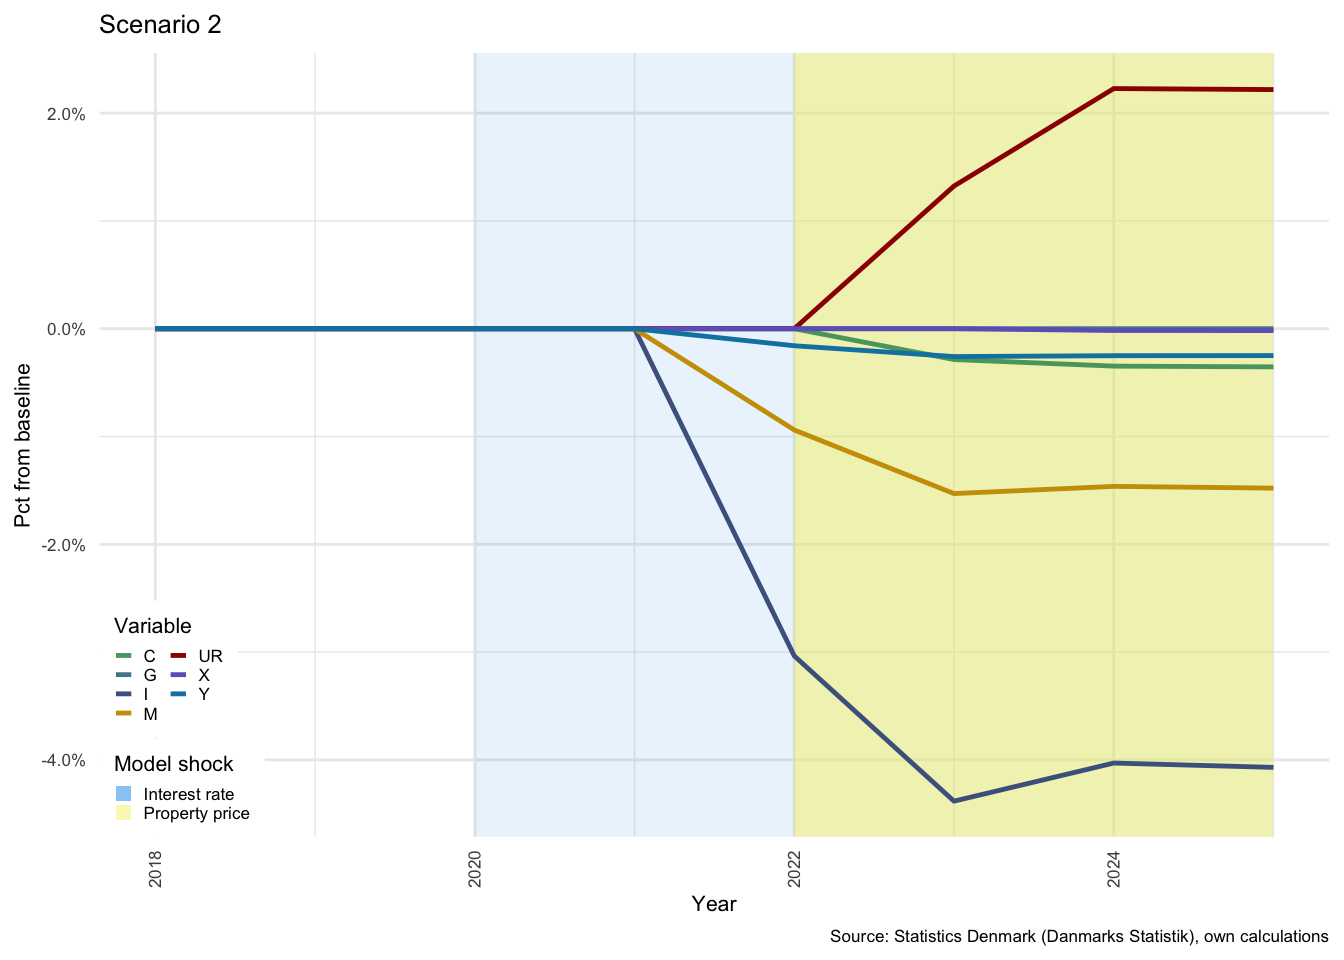
\includegraphics[width=0.5\linewidth]{figures/fl-fi-sfc-plot-gdp-indicators-s1-s2-2} \caption{National income indicators - Scenarios 1 and 2}\label{fig:fl-fi-sfc-plot-gdp-indicators-s1-s2}
\end{figure}

As described above, Scenarios 3 and 4 illustrate the compound effect of the two shocks under two different household debt positions. In Scenarios 1 to 3, proportion of fixed-interest debt (\(\alpha\)) is 38.91\%, in Scenario 4, \(\alpha\) is set to 80\%. The primary impact of this shift is a reduction in the sensitivity of household disposable income to a dramatic rise in interest rates.

As expected, the effects of the combination of the two shocks are significantly dampened when \(\alpha\) is higher. This is clear from the scales in Figure \ref{fig:fl-fi-sfc-plot-gdp-indicators_s3_s4}, where on the left for Scenario 3, investment drops just below -6\% compared with -5.5\% on the right for Scenario 4. This pattern repeats itself throughout this results section.

\begin{figure}[H]
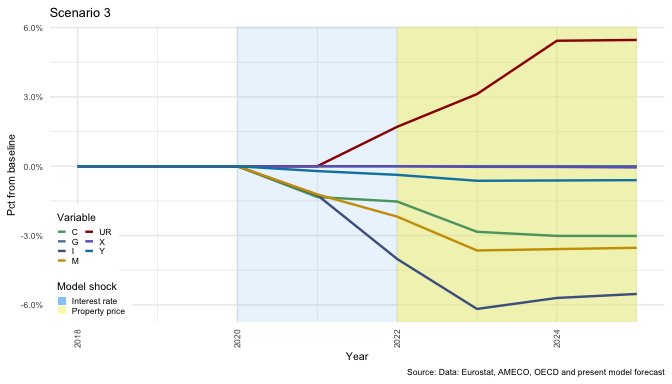
\includegraphics[width=0.5\linewidth]{figures/fl-fi-sfc-plot-gdp-indicators-s3-s4-1} 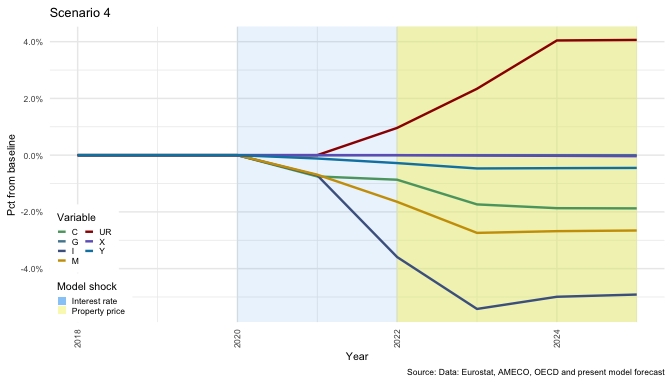
\includegraphics[width=0.5\linewidth]{figures/fl-fi-sfc-plot-gdp-indicators-s3-s4-2} \caption{National income indicators - Scenarios 3 and 4}\label{fig:fl-fi-sfc-plot-gdp-indicators-s3-s4}
\end{figure}

GDP is also somewhat better protected from the shock in the latter case. The unemployment rate (\(UR\)) increase is a compound effect of the two shocks, and is also significantly higher in Scenario 3 than in Scenario 4. The number of persons employed are determined by the NFC, and is a function of the level of \(Y\) in the previous period and changes in the size of the labour force. Exogenous growth in the size of the labour force combined with a decline in economic activity, drive the proportion of unemployed persons upwards. This also results in a rise in the level of social benefits drawn by HH from GOV, but this will be discussed in the sections for each sector below.

In many of the charts that follow, all scenarios are displayed for each of the variables. This allows for a comparison of the impact of the shocks. The baseline scenario is illustrated by a solid black line, Scenario 1 by a light-grey, dashed line. Scenario 2 by a medium-dark-grey, dashed line. Scenario 3 by the dark-grey short-dashed line and Scenario 4 by the red short-dashed line.

For each sector we will highlight the components that move most dramatically for shocks 1 and 2, and thereafter will focus on the comparative difference of these effects in Scenarios 3 and 4. This highlights the major transmissions for each shock in each sector. It also allows us to compare the impact of a hypothetical change in the allocation of debt between fixed- and flexible-interest rate products. Essentially we are able to show the impact of financial innovations, within the bounds of the assumptions discussed above.

A summary of the impact of the shocks, as captured by the net financing requirements (Net lending, \(NL\)) of each sector for each year following the shocks, can be seen in Figure \ref{fig:fl-fi-sfc-plot-nl-S1-S4}.

\begin{figure}[H]
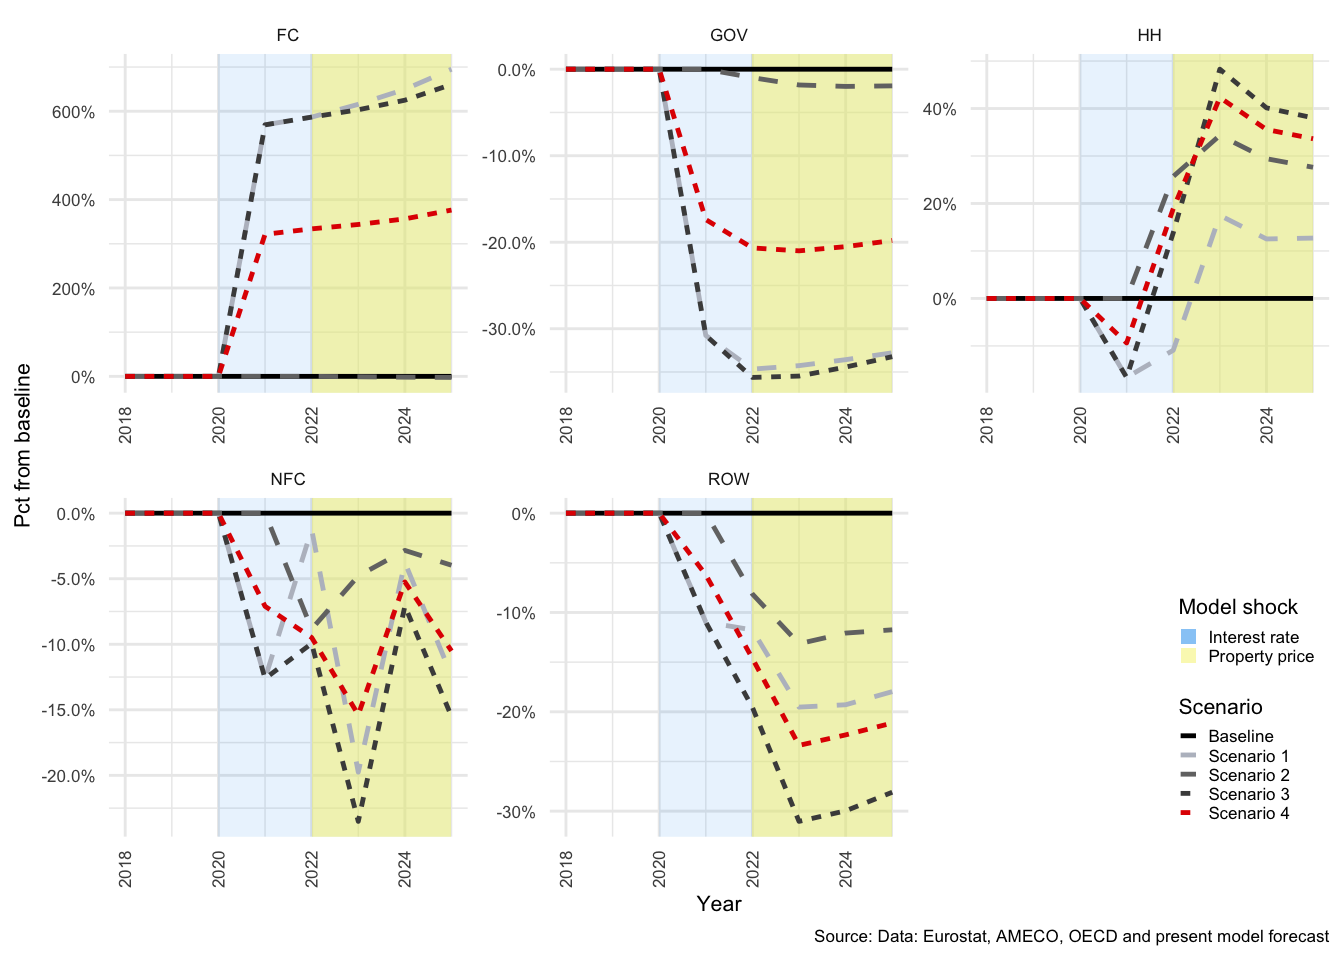
\includegraphics[width=0.95\linewidth]{figures/fl-fi-sfc-plot-nl-S1-S4-1} \caption{Net lending}\label{fig:fl-fi-sfc-plot-nl-S1-S4}
\end{figure}

Base purely on \(NL\), as shown in Figure \ref{fig:fl-fi-sfc-plot-nl-S1-S4}, it would appear that HH are net borrowers (have negative \(NL\)) as a result of the interest rate rise, as might be expected, but rather counter-intuitively\footnote{This result is perfectly logical in the context of the model, but at first glance appears to be illogical.} move into a strong net lending position following the property price collapse in 2022. ROW moves into positive \(NL\) in all scenarios, as does FC, with the exception of Scenario 2, which leaves FC \(NL\) unchanged. The scale of the changes in FC's \(NL\) are a cause for concern, and will be addressed in the FC section below. NFC and GOV move into negative \(NL\) in all circumstances, but NFC has much more erratic movements.

For all sectors, Scenario 4 is again similar to Scenario 3, but with significantly less dramatic effects. The next section will help to highlight a problem with a focus purely on \(NL\). In summary, such a focus may not be indicative of the actual economic consequences of these shocks for each sector.

For each sector the analysis includes a brief summary the most affected components from each shock, plus a graphical analysis of the most important transmission channels. For Scenario 1, these can be seen in Tables \ref{tab:most-affected-scenario-1-perc-2020-economy} to \ref{tab:most-affected-scenario-1-perc-2020-ROW} for (\(t + 1\)) 2021, and Tables \ref{tab:most-affected-scenario-1-perc-2023-economy} to \ref{tab:most-affected-scenario-1-perc-2023-ROW} for (\(t+3\)), which is 2023.

For Scenario 2, they can be seen in Tables \ref{tab:most-affected-scenario-2-perc-economy} to \ref{tab:most-affected-scenario-2-perc-ROW} for 2022, and Tables \ref{tab:most-affected-scenario-2-perc-2025-economy} to \ref{tab:most-affected-scenario-2-perc-2025-ROW} for (\(t+3\)), which is 2025. Similar tables can be seen for Scenarios 3 and 4 from Table \ref{tab:most-affected-Scenario-3-perc-economy} to Table \ref{tab:most-affected-Scenario-4-2025-perc-ROW}, where the effects are summarised for the years 2021, which allows for a comparison of the first shock, and 2025, which captures the difference in the compound effect of both shocks.

\hypertarget{effects-for-the-hh-sector}{%
\subsection{Effects for the HH sector}\label{effects-for-the-hh-sector}}

For HH, in 2021, the most obvious effect of the first shock is the increase in interest paid on mortgage debt (or property income paid) of 95.85\%. The immediate reduction in transactions for new interest-bearing assets (\(\downarrow IBATR^H\)) and liabilities (\(\downarrow IBLTR^H\)) by -78.28\% and -73.94\% respectively, and transactions in equity assets (\(\downarrow EQATR^H\)) fall by -68.34\%. These are dramatic proportional shifts, largely due to the very low base of the baseline figures. These changes are not only driven by portfolio allocation decisions but also by changes in the real economy, as aggregate demand is reduced due tot he change in interest rates.

HH investment (gross fixed capital formation, \(\downarrow I^H\), which is only houses in this model) falls by -6.81\% and savings by -10.3\% (thus the decline in \(\downarrow NL\) of around -16.64\%). This follows a decline in disposable income of -2.58\% and consequently in consumption of about -1.33\%. In terms of stocks, households immediately reduce holdings of IBL by -2.26\% and IBA by -3.23\%.

The residual financial flow for HH is transactions in interest bearing assets, \(IBATR^H_t\), which are assumed to be deposits. It is directly affected by changes in the level of net lending (\(NL^H\)), changes in transactions in IBL (\(IBLTR^H_t\)), transactions in equities (\(EQATR^H_t\)) and net transactions in pension assets (\(PENATR^H_t\)). The link between new debt \(IBL^H\) and new deposits \(IBA^H\) is analogous to the PK theory of endogenous money supply since an increase in debt is associated with an increase in deposits. This is represented in Equation \ref{eq:ibatr_hh_intext}.

\begin{equation}
IBATR^H_t = NL^H + IBLTR^H_t - EQATR^H_t - PENATR^H_t
\label{eq:ibatr_hh_intext}
\end{equation}

The progression of each of these transaction flows is presented in Figure \ref{fig:fl-fi-sfc-plot-hh-indicators-ibatr} below. The decline in \(\downarrow IBATR^H\) of -78.28\% is easily discernible. The reader should note that the scale on each plot differs, and the change to \(PENATR^H\) is largely irrelevant at less than 1\%, and the declines in \(IBLTR^H\), \(EQATR^H\) and \(IBATR^H\) are of far greater interest. This is appropriate, as each item should be read independently.

Following the dark-grey dotted line describes Scenario 1, where, in all but pension asset transactions, the initial decline is dramatic, but in subsequent years there is a fairly rapid recovery. \(IBATR^H\) is represented in the top centre panel, and is the sum of the remaining four items. In Scenarios 1,3 and 4, the interest rate shock results in significant negative savings, but with the introduction of the property price collapse in 2022, for Scenarios 2 to 4, NL swings positive. This is explored further below.

Comparing Scenarios 3 (dark-grey short-dashed line) and 4 (red short-dashed line) reveals that the effect of the combination of the two shocks is 50\% smaller for Scenario 4 after the interest rate shock (shock 1), and roughly 10\% to 20\% smaller for the property shock (shock 2).

\begin{figure}[H]
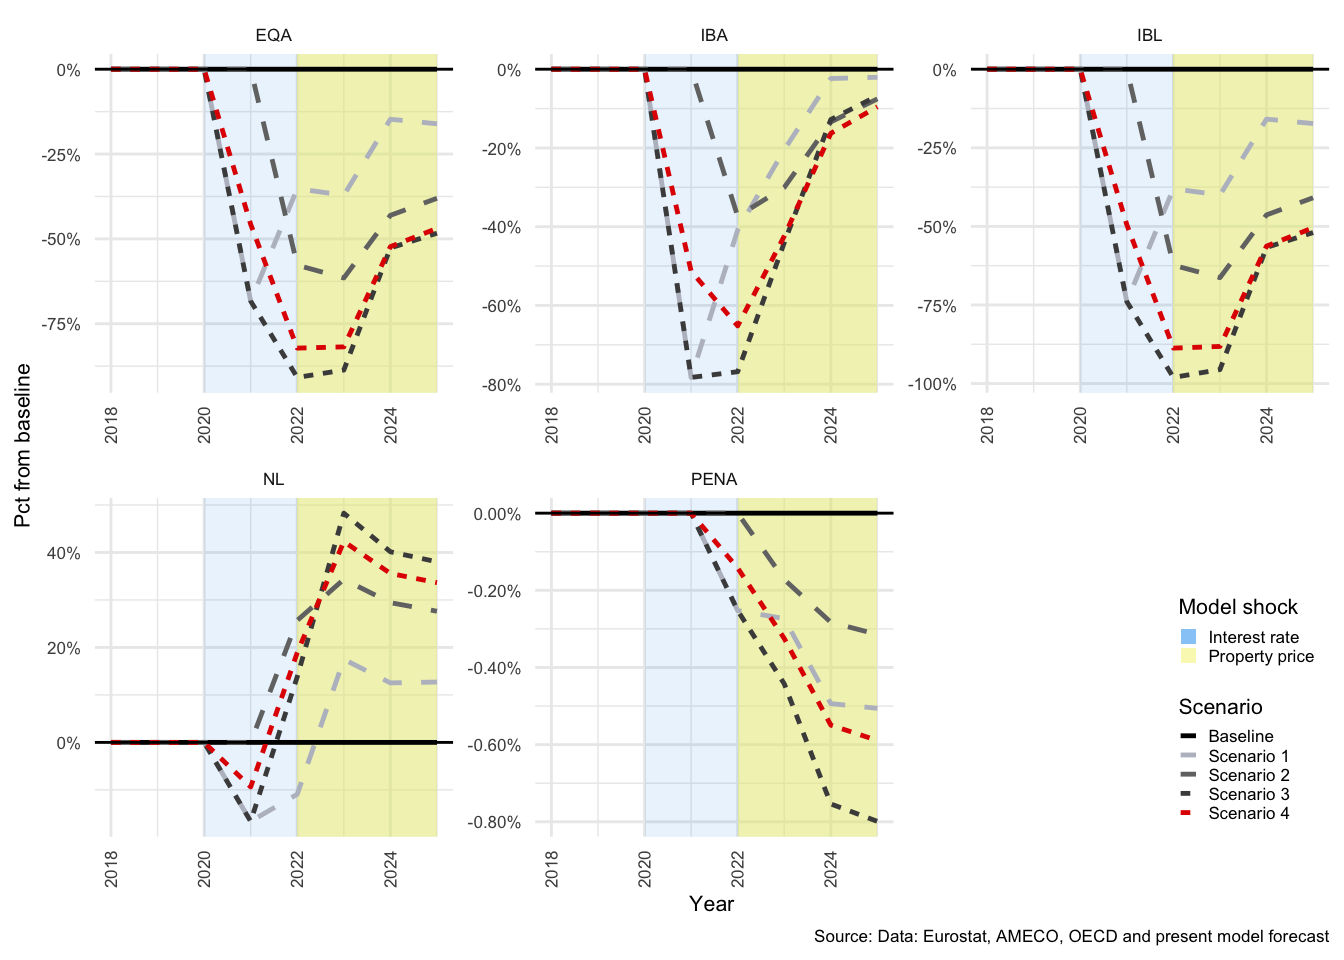
\includegraphics[width=0.95\linewidth]{figures/fl-fi-sfc-plot-hh-indicators-ibatr-1} \caption{Households: Transactions in assets}\label{fig:fl-fi-sfc-plot-hh-indicators-ibatr}
\end{figure}

The level of net lending \(NL^H_t\) is essentially driven by changes in savings (\(S^H_t\)) and investment levels (\(I^H_t\)). The changes in net purchases and sales of fixed assets (\(NP^H\)) and net capital transfers (\(KTR^H\)) are exogenous, and so do not differ from the baseline (this is repeated for all sectors). The level of net lending for HH is calculated as follows.

\begin{equation}
NL^H_t = S^H_t - I^H_t - NP^H_t + KTR^H_t
\end{equation}

The \(I^H\) and \(S^H\) components of \(NL\) can be seen in Figure \ref{fig:fl-fi-sfc-plot-hh-indicators-nl}. \(I^H\) (INV in the plot) recovers in the second period after the shock but then declines again in the fourth. \(S^H\) and \(NL\) fall by about around 10\% in Scenarios 1 and 3, but only by about half of that for Scenario 4. \(I^H\) (which is entirely in houses) declines even more dramatically in Scenarios 2 with the collapse in house prices, and this is compounded with the fall of shock 1 in Scenarios 3 and 4. There is a decline of over 30\% from baseline investment by 2023 when the level of ARM (flexible-rate mortgages) is allowed to remain high in Scenario 3.

\begin{figure}[H]
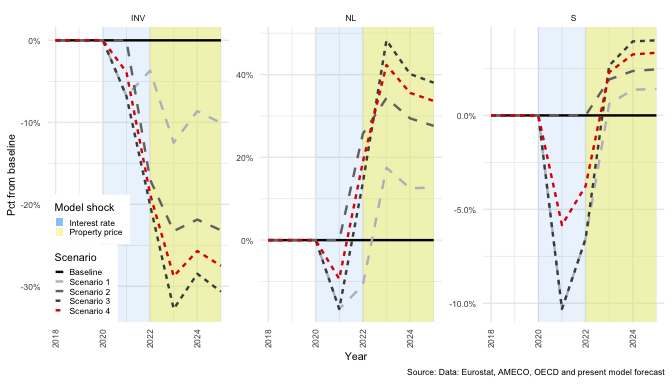
\includegraphics[width=0.95\linewidth]{figures/fl-fi-sfc-plot-hh-indicators-nl-1} \caption{Household Net Lending components}\label{fig:fl-fi-sfc-plot-hh-indicators-nl}
\end{figure}

Savings (\(S^H\)) are almost entirely determined by the level of disposable income of HH, and since the tax proportion is held constant, it is the income portion that drives most of the changes. While savings recover in the periods after the shock, investment activity declines further, which is the main driver behind the correction of \(NL\). Thus, it is unfortunately a decline in economic activity that allows for the financial recovery. The decline in \(I^H\) also means that capital formation fails to offset depreciation, and thus, HH capital levels decline.

Equation (\ref{eq:Yht-text}) describes the incomes and expenditures of HH that ultimately determine the gross income for the sector (\(Y^H_t\)). The primary sources of which are wages (\(WB^H\), W in the plot below), profits (\(B2\), which is exogenous), property income (or returns on financial capital, which stems from interest bearing assets, \(IBA^H\), pensions, \(PENA^H\), and equities, \(EQA^H\)), and social transfers (\(STR^H\), STRA in the plot below).

\begin{equation}
\begin{split}
Y^H_t = & WB^H_t + B2^H_{t} + r^H_{A_{t-1}}(IBA^H_{t-1})\\
        & - r^H_{L(FI)_{t-1}}(IBL(FI)^H_{t-1})\\
        & - r^H_{L(FL)_{t-1}}(IBL(FL)^H_{t-1})\\
        & + \chi _t(EQA^H_{t-1}) + \psi _t(PENA^H_{t-1}) + STR^H_t + \epsilon ^H
\label{eq:Yht-text}
\end{split}
\end{equation}

Interest rates are represented by \(r^H\), and the ``A'' (``L'') subscript referring to the assets (liabilities), and (\(\chi _t\)) and (\(\psi _t\)) are the rates of return on equities and pensions. As part of the key change in this model, the level of interest paid on \(IBL\) in this model is split between fixed and flexible rate mortgages into \(r^H_{L(FI)_{t-1}}(IBL(FI)^H_{t-1})\) (PIP-IBL-Fixed, in the plot below) and \(r^H_{L(FL)_{t-1}}(IBL(FL)^H_{t-1})\) (PIP-IBL-Flexible, in the plot below). A similar split is present in the financial corporate sector (FC) below.

The \(\epsilon ^H\) refers to adjustments made to ensure stock and flow consistency in the level of property income received or paid during the periods where data was available\footnote{This convention is used for all sectors. The returns on financial assets are estimated with varying degrees of accuracy for each of the sectors. In order to ensure that the model is consistent in all periods, any difference between the estimated returns and actual returns (on a net basis for each asset class) are added to the adjustment term. These errors in estimation are minimised in the estimation specification for each asset class individually.}.

Figure \ref{fig:fl-fi-sfc-plot-hh-indicators-y} displays the endogenous components of HH income. Property income received on financial assets, are labelled PIR-EQA for \(EQA^H\), PIR-IBA for \(IBA^H\), PIR-PENA for \(PENA^H\). PIP-IBL is the sum of interest paid on \(IBL(FI)^H\) and \(IBL(FL)^H\), which is all interest paid on mortgage debt. Also included in the figure are consumption (\(C^H\)) and income tax (\(T^H\), TAX in the plot below).

\begin{figure}[H]
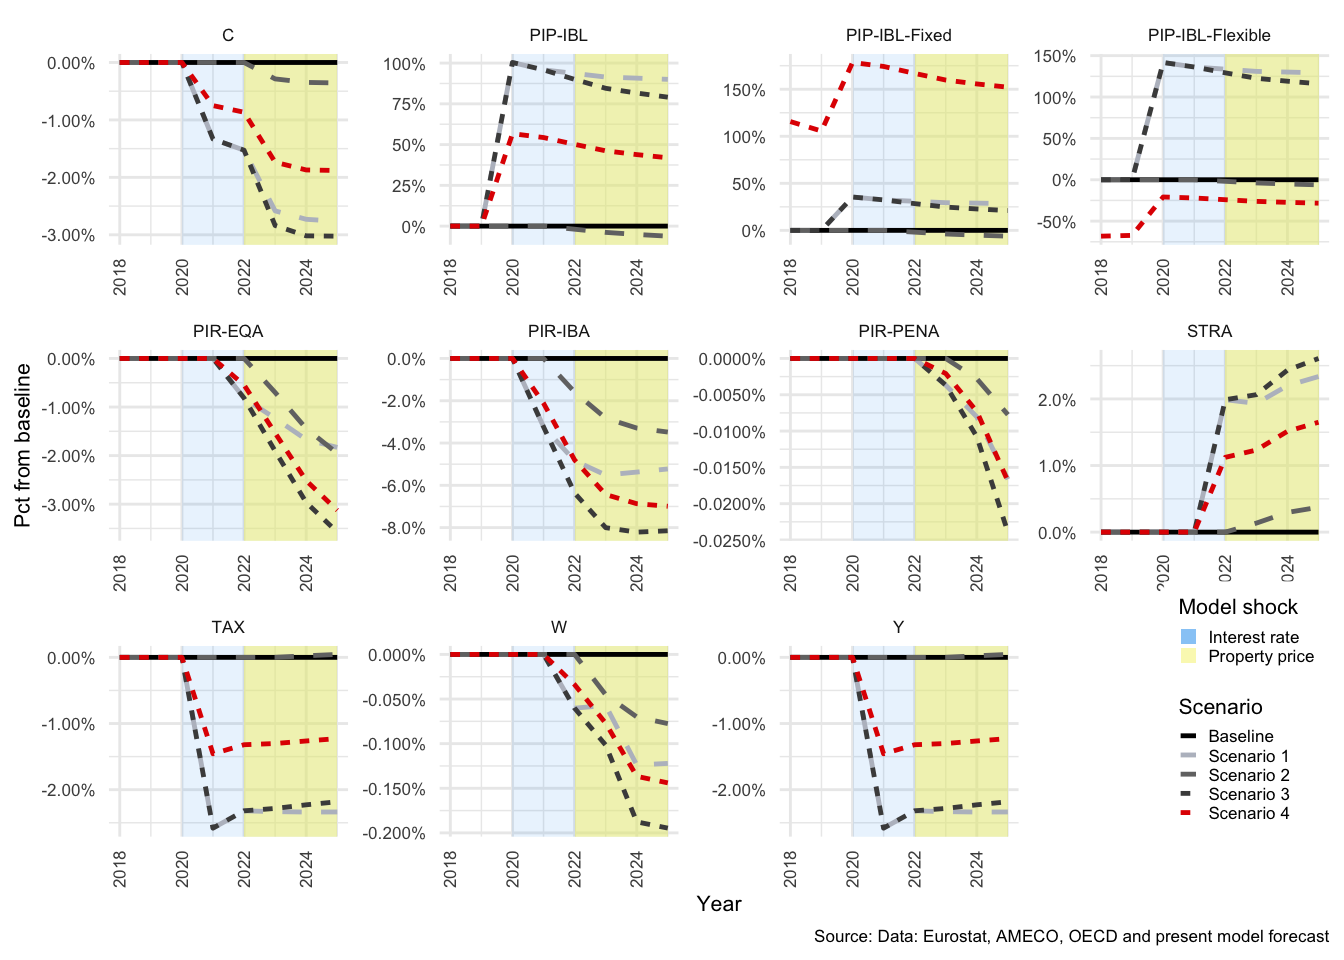
\includegraphics[width=0.95\linewidth]{figures/fl-fi-sfc-plot-hh-indicators-y-1} \caption{Household income components}\label{fig:fl-fi-sfc-plot-hh-indicators-y}
\end{figure}

The sum of all changes in the model accumulate in the level of \(Y^H\) in the bottom right hand panel of Figure \ref{fig:fl-fi-sfc-plot-hh-indicators-y}, Scenario 2 has almost zero impact on \(Y^H\), while Scenarios 1, 3 and 4, which include the interest rate change, all result in a significant net decline. PIP-IBL, in the panel to the right of consumption (\(C\)) in the top left corner, is the total interest paid on debt by HH, and highlights the most dramatic change. It also illustrates the key difference introduced in Scenario 4, which is a reduction in the sensitivity of HH income to changes in interest rates relative to Scenario 3.

The largest contributors to HH income are wages (\(W^H\)) and social transfers (\(STR^H\), STRA in the plot above). Since 2007, approximately 35\% to 37\% of social transfers represent a tax funded pension income, and most of the remainder covers medical and disability support\footnote{Based on data from Statistics Denmark, since 2007, approximately 35\% - 37\% of all social benefits
  were for old age payments. A further 20\% - 22.3\% are attributed to medical benefits, an almost
  constant 14.4\% to disability and 10\% - 13.2\% to family and child benefits. Unemployment (app. 5\%),
  social exclusion (app. 5\%), housing (app. 2\%) and survivorship (app. 1\%) benefits making up the balance. The bulk of these transfers can be thought of as supplementary income, rather than unemployment support.}. To give a sense of scale, Figure \ref{fig:fl-fi-sfc-plot-hh-indicators-npir} shows the actual values of the major contributors, where NPIR is a net sum of all property income received and paid, and remains positive, but falls by roughly 50\% due to the rise in interest costs on mortgages\footnote{The impact of the shift in \(\alpha\) can be seen in the two panels to the top right. PIP-IBL-Fixed, and PIP-IBL-Flexible are drastically different in Scenario 4 to all other Scenarios. This is because Scenarios 1 to 3 all keep the baseline allocations of debt between fixed and flexible. The difference from baseline illustrated in Figure \ref{fig:fl-fi-sfc-plot-hh-indicators-y} above are predominantly due to the change in \(\alpha\) in 2017 - hence the separation prior to the first shock in 2020.}.

Wages (\(W\)), taxes (\(T^H\), TAX) and consumption (\(C\)) all decline with \(Y^H\).

\begin{figure}[H]
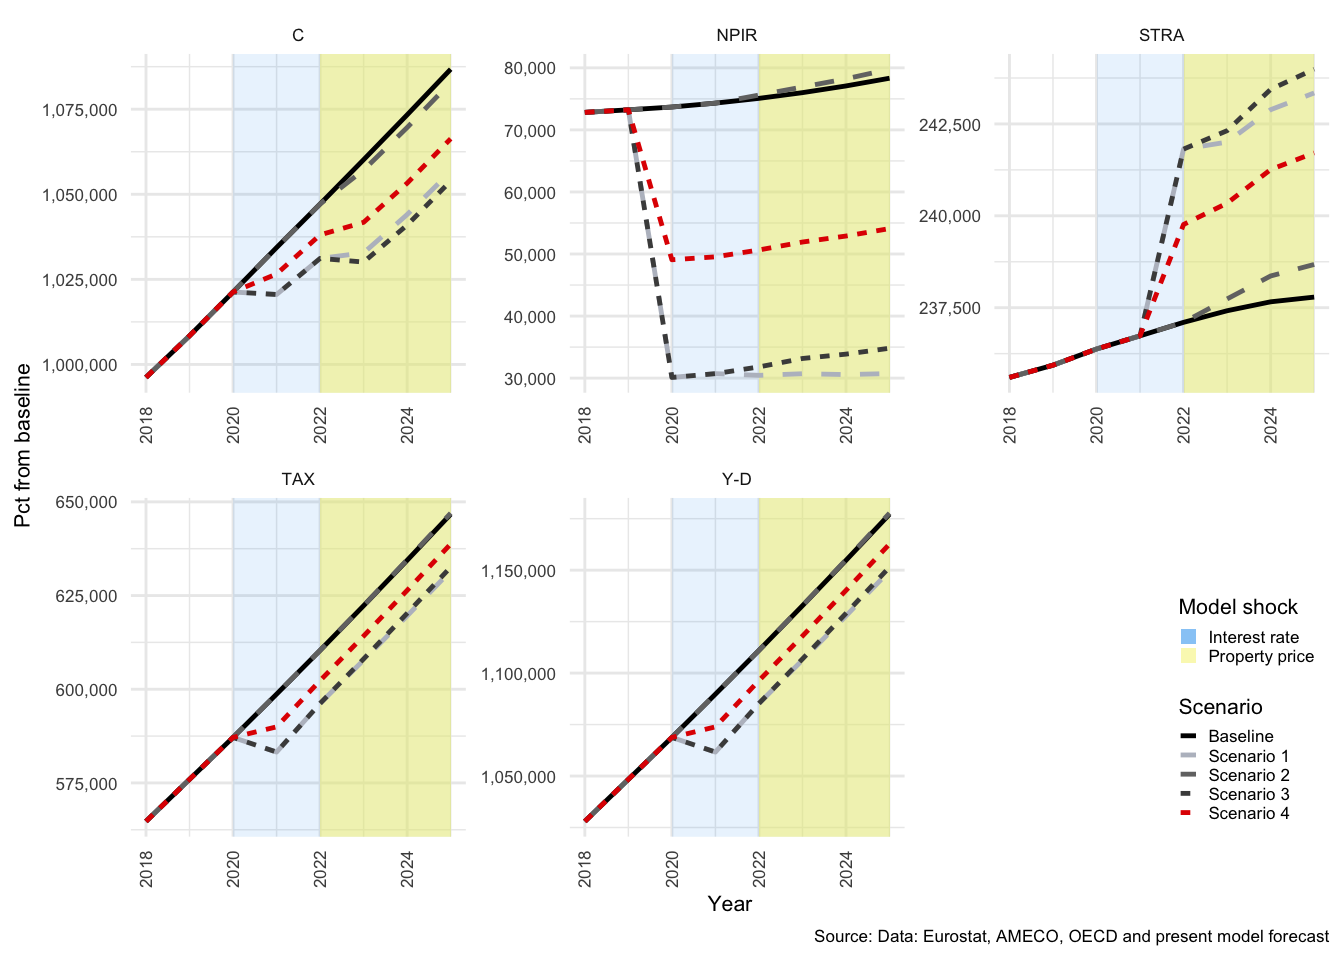
\includegraphics[width=0.95\linewidth]{figures/fl-fi-sfc-plot-hh-indicators-npir-1} \caption{Household savings components}\label{fig:fl-fi-sfc-plot-hh-indicators-npir}
\end{figure}

From this it is possible to see that the rise in \(STR^H\) is not sufficient to offset the fall in property income. Scenario 2 is the obvious exception, where income rises marginally. Disposable income (\(Y_d\), shown as Y-D above) declines in Scenarios 1 and 3, but in Scenario 4 only stagnates before trending upwards again. The trend in consumption follows the shift in \(Y_d\). The effects of the shocks on the HH financial balance sheet can be seen in Figure \ref{fig:fl-fi-sfc-plot-hh-bs}.

\begin{figure}[H]
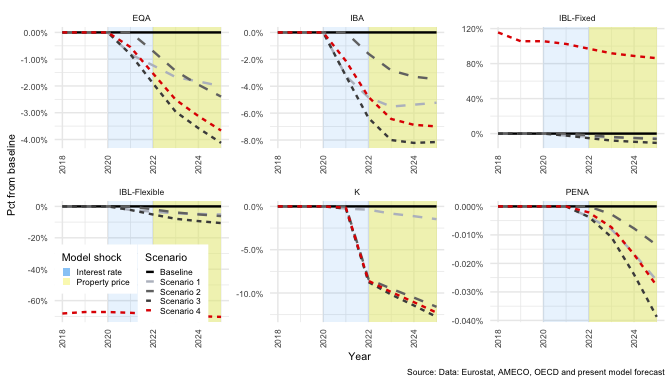
\includegraphics[width=0.95\linewidth]{figures/fl-fi-sfc-plot-hh-bs-1} \caption{Household balance sheet}\label{fig:fl-fi-sfc-plot-hh-bs}
\end{figure}

The decline in \(PENA\) are negligible relative to the baseline, but the decline in capital (\(K^H\)) that occurs due to the shock to housing prices, has a significant impact on both consumption and investment in subsequent periods. The consequence of the rise in interest rates, and decline in housing investment can be seen in the panel for \(K\) above, where Scenario 1 shows a gradual decline relative to the baseline. The impact of a shock to housing prices, however, has a far more dramatic impact in 2022.

In the scenario three, three years after the compounding of the property price decline, net HH wealth falls by 3.34\%, but this understates the impact on the HH, since, as mentioned in the introduction, net measurements fail to take into account the impact on gross balances. In gross terms, stock of interest bearing liabilities falls by 10.6\%, HH wealth in financial assets falls by 3.55\% while stock of capital held in houses falls by 12.76\%. These are substantial declines in the total level of wealth, but probably overstates the effect on property, since although property prices are allowed rise gradually, the recovery is more gradual that was observed for the Danish economy. The contraction in liabilites is also substantially higher than the modest effect observed over the GFC. One major difference, however, is that HH benefitted from global suppression of interest rates, which would be quite the opposite if interest rates were to rise.

In summary, on the basis of the model, an interest rate hike and a collapse in property prices would both force the HH balance sheet to contract. The main transmission channel that this would occur through is a direct reduction in disposable income due to debt costs, or the credit channel. It also shows that if it were possible to instigate a change in the composition of debt from flexible- towards fixed-interest products, the lower sensitivity of fixed-rate debt products might protect HH from the majority of these impacts.

\hypertarget{effects-for-the-nfc-sector}{%
\subsection{Effects for the NFC sector}\label{effects-for-the-nfc-sector}}

The changes in Scenario 1 for NFC are rather limited at first, as can be seen in Table \ref{tab:most-affected-scenario-1-perc-2020-NFC}, but by 2023, as shown in Table \ref{tab:most-affected-scenario-1-perc-2023-NFC}, the effects of the shocks have spread far enough that changes in real economic activity have an impact on the level of employment and output.

In 2021 \(NIBTR^N\) falls by -12.62\%, which is equal to the fall in \(NL\). \(S^N\) falls by -1.1\%, \(T^N\) by -0.2\%
and profits (\(B2^N\)) by -0.19\%.

By 2023 the real economy effects feed into NFC, and \(NIBTR^N\) has fallen by -19.75\%, which is equal to the fall in \(NL\). \(I^N\) has fallen by -0.22\%, and \(S^N\) by -1.61\%. \(T^N\) by -0.33\% and profits (\(B2^N\)) by -0.31\%. The net flow of all property income is -0.17\% lower and the stock of \(NIB^N\) is -1.48\% lower than baseline. There is also a -0.08\% fall in total capital of NFC.

NFC's residual financial flow is \(NIBTR^N\), and the contributors to it are net lending (\(NL^N\)) and net equity transactions (\(NEQTR^N\)). Unlike the household sector, the financial activity of the NFC is not modelled directly, and \(NEQTR^N\) are therefore exogenously determined for periods where data is available, and revert exogenously to zero for all periods of estimation. \(NIBTR^N\) therefore depend only on \(NL\).

\begin{equation}
NIBTR^N_t = NL^N_t - NEQTR^N_t
\end{equation}

Net lending again depends on Savings and investment,

\begin{equation}
NL^N_t = S^N_t - I^N_t- NP^N_t + KTR^N
\end{equation}

Investment is estimated in real terms, and is positively dependent on real gross income (\(y_{t-i}\)), and negatively dependent on the real level of capital (\(k^N_{t-i}\)), each with a variable number of lags in the estimate\footnote{In this versions of the model, \(k^N_{t-i}\) and \(y_{t-i}\) are both estimated at \(t-1\), together with a significant dummy variable for 2009.}. In this context, the proportion, \(\Bigg( \frac{y_{t-i}}{k^N_{t-i}} \Bigg)\), represents capacity utilisation.

\begin{equation}
ln(i^N_t) = \beta _i + ln\beta _i \Bigg( \frac{y_{t-i}}{k^N_{t-i}}\Bigg)
\end{equation}

\begin{figure}
\centering
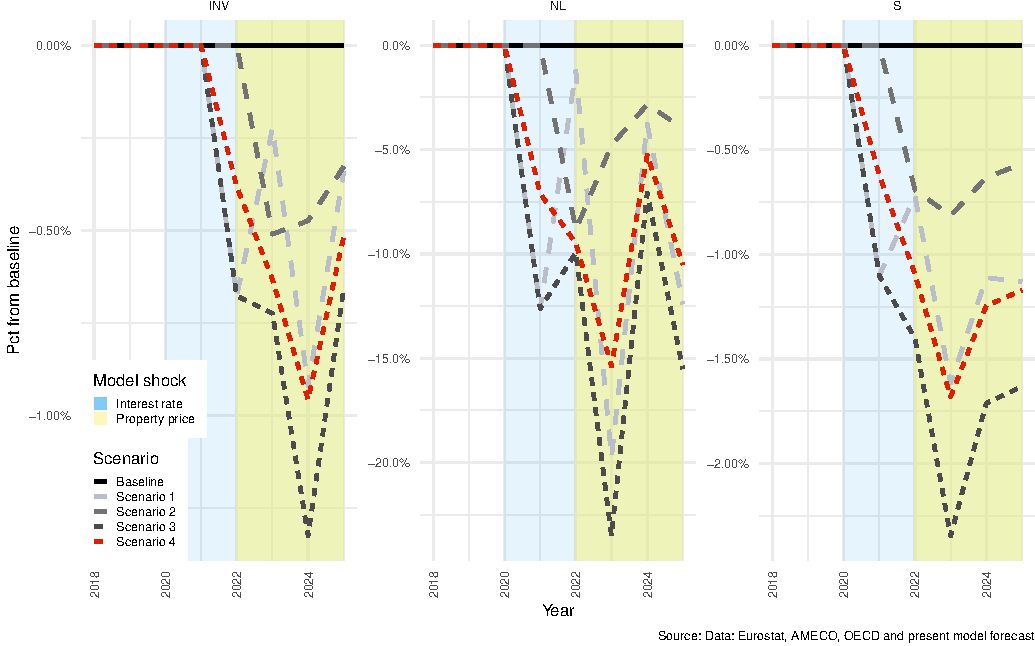
\includegraphics{figures/fl-fi-sfc-plot-nfc-indicators-nl-1.pdf}
\caption{\label{fig:fl-fi-sfc-plot-nfc-indicators-nl}NFC Net Lending components}
\end{figure}

The major determinants of investment are therefore the major determinants of GDP, together with previous capital accumulation in NFC (previous capital, plus investment less depreciation). As can be seen in Figure \ref{fig:fl-fi-sfc-plot-nfc-indicators-nl}, \(I^N\) (INV in the plot) is fist affected by Scenario 1 (interest rates) in 2022, this the change in NL observable is 2021 is purely due to the decline in savings. Although the shapes of the panels in Figure \ref{fig:fl-fi-sfc-plot-nfc-indicators-nl} are very similar, the scales are quite different. The actual underlying values of each category are also significantly different. Plotted as actual values in Figure \ref{fig:fl-fi-sfc-plot-nfc-indicators-nl-actuals}, the changes would be almost indiscernible from the baseline.

\begin{figure}
\centering
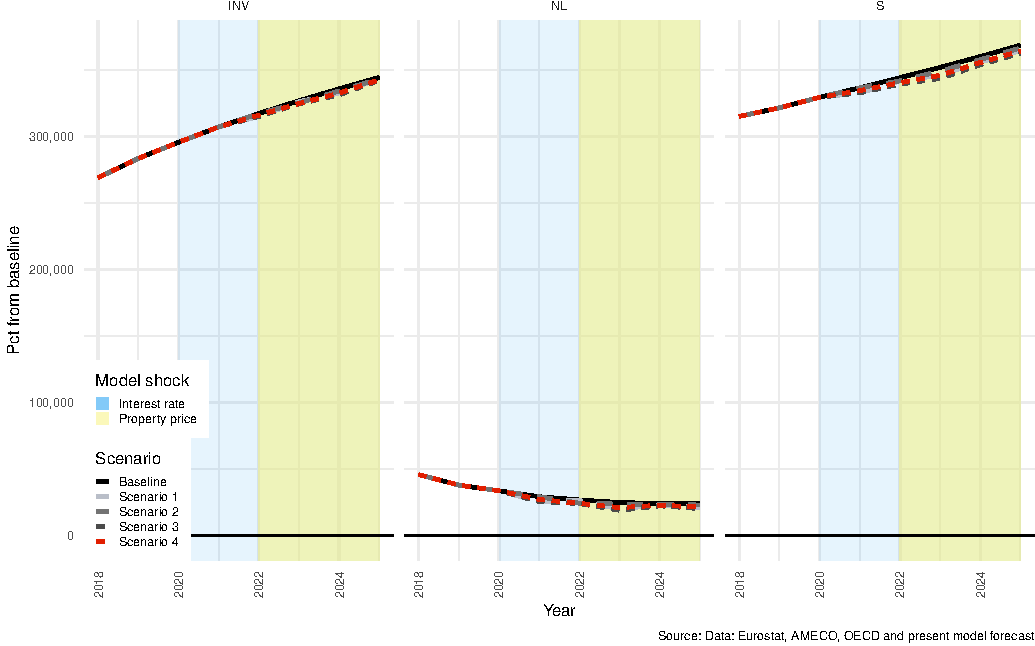
\includegraphics{figures/fl-fi-sfc-plot-nfc-indicators-nl-actuals-1.pdf}
\caption{\label{fig:fl-fi-sfc-plot-nfc-indicators-nl-actuals}NFC Net Lending components}
\end{figure}

NFC savings (\(S^N_t\)), can be calculated as the net sum primary and secondary income and expenditures.

\begin{equation}
\begin{split}
S^N_t = & Y_t - WB^N_t + (B2^N_{t} - B2_{t}) + r^N_{t-1}(NIB^N_{t-1})\\
        & + \chi _t (NEQ^N_{t-1}) - T^N_t + STR^N_t + \epsilon ^N
\end{split}
\end{equation}

\(NPIR-NEQ\) and \(STRA\) are exogenous, and revert to zero values after the last period of available data, 2017.

\begin{figure}
\centering
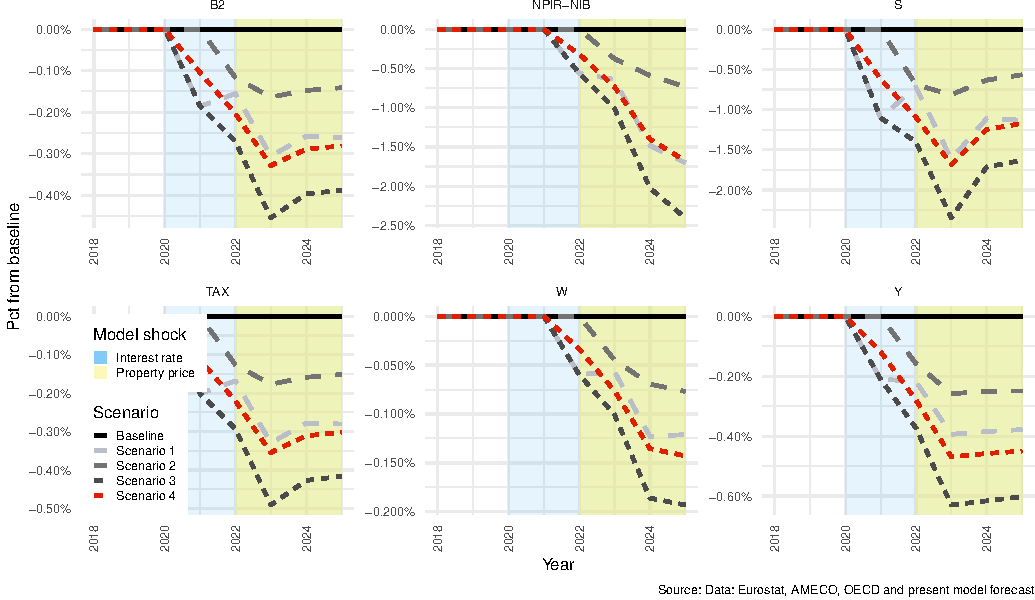
\includegraphics{figures/fl-fi-sfc-plot-nfc-indicators-saving-1.pdf}
\caption{\label{fig:fl-fi-sfc-plot-nfc-indicators-saving}NFC Savings components}
\end{figure}

\hypertarget{effects-for-the-gov-sector}{%
\subsection{Effects for the GOV sector}\label{effects-for-the-gov-sector}}

For Scenario 1, in 2021 \(NIBTR^G\) is -30.78 \% lower than the baseline. The source of this decline can be traced through the plots below. Figure \ref{fig:fl-fi-sfc-plot-GOV-indicators-nl} shows the decline in net lending and savings.

Contributing to the decline in \(NL^G\) is a decline of -11.85\% in \(S^G\). The main contributor to which is a fall in \(T^G\) of -1.56\%. The net issue of \(IBL\) results in a fall in \(NIB^G\) of -9.16\% and for net wealth to decline by -1.3\%.

By 2023 the first shock has spread through the economy and \(NL\) is -34.27\% below the baseline levels. The delayed effect of the change in interest rates is by that stage in effect, and results in a decline in net property income of -15.36\%. This contributes to a reduced level of \(S^G\) of -14.07\% below. The major contributor is a -1.47\% lower level of tax revenue.

Social transfers for each sector, \(STRA^G\) in the case of GOV, are a net value of receipts less payments. \(STRA^G\) declines by -1.21\%, indicating that the level of payments has increased relative to receipts. This contributes further to the negative balance in GOV. The decline in \(NIBTR^G\) above accumulates in \(NIB^G\) that is -19.27\% lower than the baseline, and net wealth, \(NW^G\), that is -4.02\% lower.

Shock 2 in 2022, the property price decline, has very little impact on GOV, with only a marginal decline in \(S^G\), flowing from limited impacts to the underlying components. \(NL^G\) falls by only -0.97\%. This since tax revenues are only marginally affected when HH disposable income remains fairly constant, and the ultimate effect on \(NIB^G\) is only -0.24\%. In reality this could have been substantially worse if the property price collapse resulted in non-performing loans and GOV was required to step in, as was the case for the banking crisis in Sweden in 1993. \citep{englund1999}

By 2025, the effects remain modest, with \(NL^G\) only -1.93\% down from the baseline level, and \(NW^G\) only -0.27\% lower.

The largest changes in Scenario 1 for GOV in 2021 are in the residual financial flow for GOV, transactions in net interest bearing assets (\(NIBTR^G\)). These changes come almost entirely from changes in \(NL\), another term for which would be a government deficit or surplus, for negative and positive \(NL\) respectively. GOV issues debt (\(NIBTR^G\)) to cover the deficit. These assets are accumulated by FC (below), together with property income flows according to the return on these assets (\(r_N\)). As can be seen from Equation (\ref{eq:nibtrg_intext}) below,

\begin{equation}
NIBTR^G_t = NL^G_t
\label{eq:nibtrg_intext}
\end{equation}

Government investment (\(I^G\)), (and, as with NFC) \(NP^G\) and \(KTR^G\) are exogenous, so in Equation (\ref{eq:NL_G_intext}) below, it is only changes in savings (\(S^G\)) that are influential after the shocks in each scenario.

\begin{equation}
NL^G_t = S^G_t - I^G_t - NP^G_t + KTR^G_t
\label{eq:NL_G_intext}
\end{equation}

\begin{figure}[H]
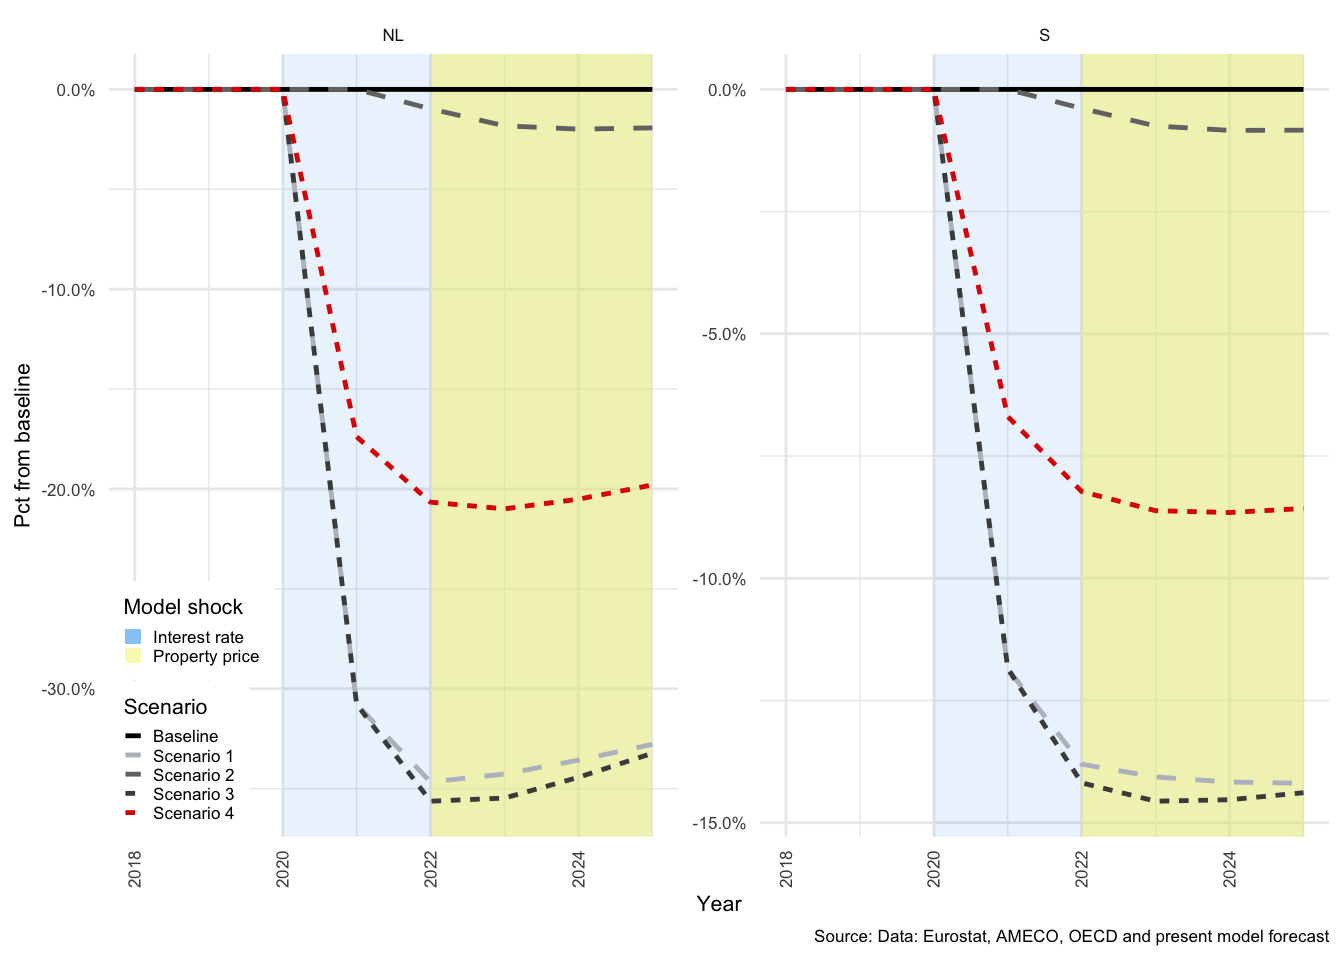
\includegraphics[width=0.95\linewidth]{figures/fl-fi-sfc-plot-GOV-indicators-nl-1} \caption{GOV Net Lending components}\label{fig:fl-fi-sfc-plot-GOV-indicators-nl}
\end{figure}

Equation (\ref{eq:savings_G_intext}) highlights the core components of GOV income. Of these \(B2^G\)+ net property income received, (\(r_{N_{t-1}}(NIB^G_{t-1})\), and NPIR in the plot below) and tax \(T^G\) are the incomes received by GOV. Social transfers (\(STR^G\), STRA in the plot below) and GOV expenditure (\(G\)). The exogenous component from the incomes is \(B2\), and from expenditure \(G\).

\begin{equation}
S^G_t= B2^G_t + r_{N_{t-1}}(NIB^G_{t-1}) + T^G_t+ STR^G_t - G_t + \epsilon ^G
\label{eq:savings_G_intext}
\end{equation}

\begin{figure}[H]
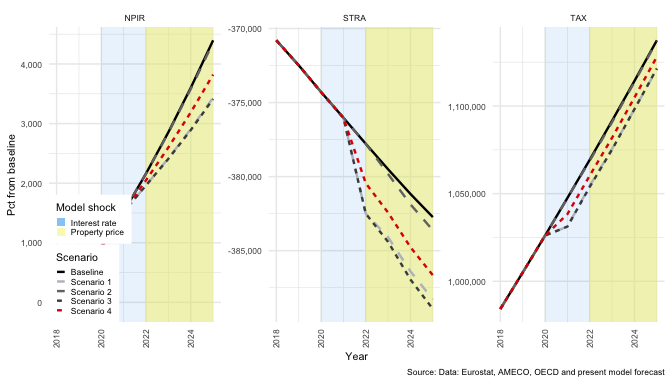
\includegraphics[width=0.95\linewidth]{figures/fl-fi-sfc-plot-GOV-indicators-savings-1} \caption{GOV Savings components}\label{fig:fl-fi-sfc-plot-GOV-indicators-savings}
\end{figure}

Considering Scenarios 3 and 4, the difference in the impact of shocks is about half as strong for Scenario 4, where \(\alpha\) is at 80\%. Scenarios 1 and 3 however result in stronger effects. The impacts to GOV are directly a result of the deterioration in HH cash flows and needs for social support. While \(STR^G\) is the expenditure of GOV that flows to HH, based on total net benefit and contribution flows. Rising \(STR^G\) expenses are exacerbated by a fall in revenues in the form of both net property income received (NPIR) and taxation \(T^G\) (TAX in the plot above.)

\hypertarget{effects-for-the-row-sector}{%
\subsection{Effects for the ROW sector}\label{effects-for-the-row-sector}}

The ROW sector is primarily driven by exports, which are exogenous, and imports, which are endogenous to changes in the level of household income. The sharp decline in household income causes an immediate improvement in the current account balance, which is reflected as a negative NL balance for ROW\footnote{The flows for ROW are recorded from the perspective of ROW. Thus, if ROW net-lends, it is the same as to say that Denmark net borrows. A positive current account for Denmark is therefore the equivalent of a net borrowing (or, negative net lending) position for ROW.}.

For shock 1, in 2021, ROW is driven into a further deficit to Denmark, with a decline of -10.97\% in \(NIBTR^W\), which captures the -10.97\% decline in \(NL^W\) and \(S^W\). This has a negative effect of -0.7\% on the level of net wealth (\(NW^W\)) held by ROW in Denmark.

The deficit in \(NL^W\) continues to grow, and by 2023 is -10.97\% lower than the baseline value. The net flow of property income on all financial assets is lower by \%, which reflects a -1.21\% fall in the stock of \(NIB^W\). From a balance sheet perspective, there is a decline of -0.7\% in net wealth (\(NW^W\)).

The second shock, to property prices has less of an impact on ROW, with \(NIBTR^W\) still lower, but in 2022, this is only by -8.14\%. This is again driven by an equal decline in \(S^W\), which leads to an equal decline in \(NL^W\). The fall in \(NIBTR^W\) is reflected as a decline in \(NIB^W\) by -0.87\%.

By 2025, the shock has spread through the economy, and the impact on \(S^W\), \(NL^W\) and \(NIBTR^W\) is lower again at -11.74\% less than the baseline value. The changes in interest earning assets reduce the level of property income from \(NIB^W\) by -3.14\%, and from all financial assets by -1.71\%. The level of \(NIB^W\) continues to fall further into deficit by -3.98\% relative to the baseline. After the three year period of accumulative effects, \(NW^W\) would be -2.69\% lower.

The transmission of these shocks, working backwards from the accumulative effect on transactions in \(NIB^W\), begins with Equation (\ref{eq:NIBTR_row_intext}).

\begin{equation}
NIBTR^W_t = NL^W_t - NEQTR^W_t - NPENTR^W_t
\label{eq:NIBTR_row_intext}
\end{equation}

Equation (\ref{eq:NIBTR_row_intext}) describes the source of changes in \(NIBTR^W\), where \(NEQTR^W\) and \(NPENTR^W\) are exogenous in the model. This leaves only \(NL\) as a possible source of change. Unlike the domestic sectors, ROW is assumed not invest in the domestic economy, which means that the net lending function is somewhat simpler, with only savings as the possible source of change.

\begin{figure}[H]
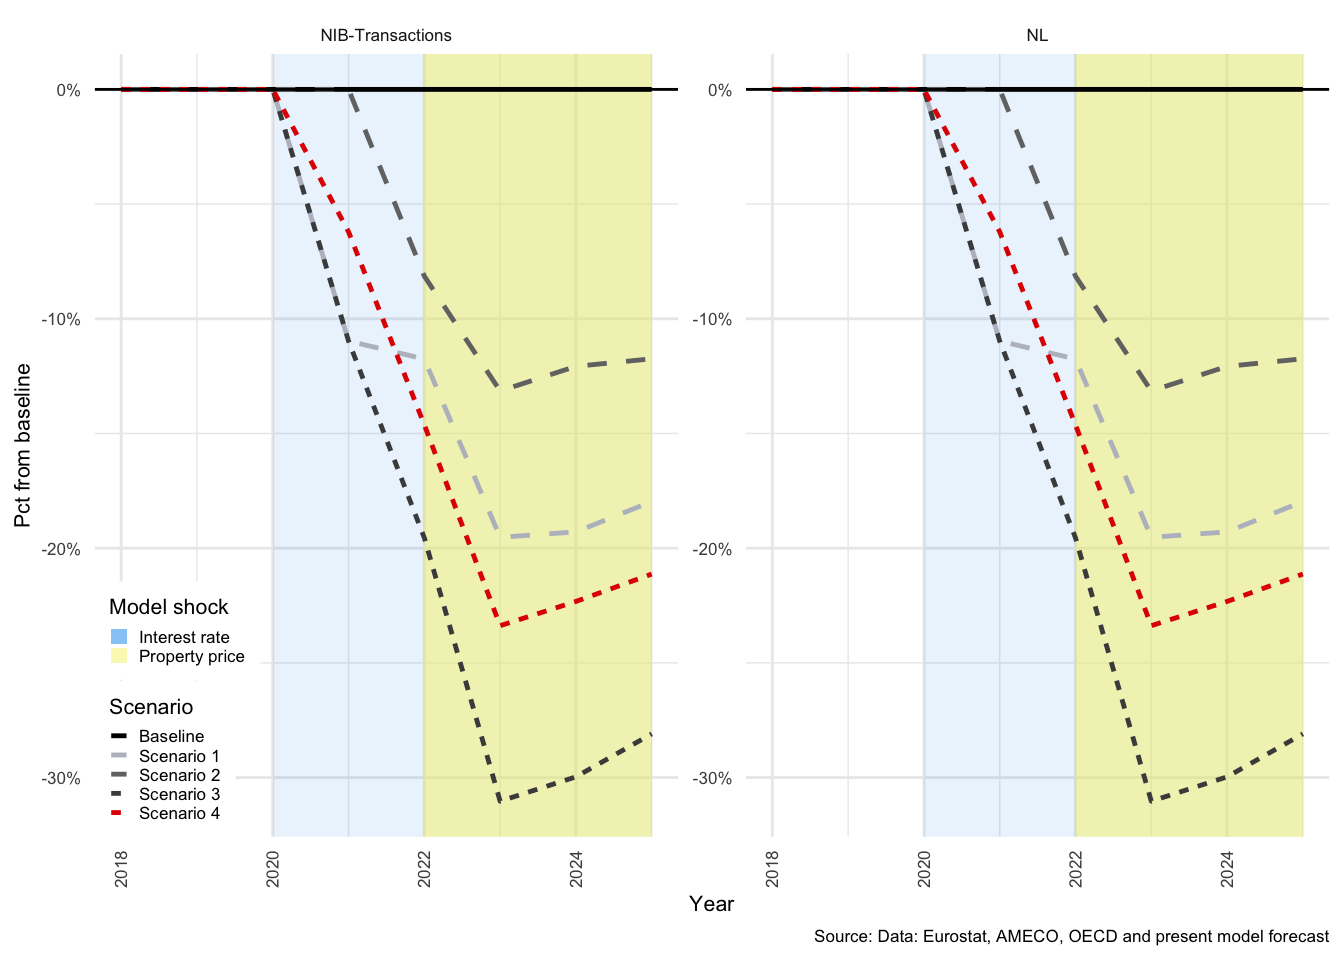
\includegraphics[width=0.7\linewidth]{figures/fl-fi-sfc-plot-row-indicators-nibtr-1} \caption{ROW: NIBTR: Transactions in assets and net lending}\label{fig:fl-fi-sfc-plot-row-indicators-nibtr}
\end{figure}

Equation (\ref{eq:NL_row_intext}) highlights the components of \(NL\), and much like the previous sectors, only \(S^W\) is endogenous in the model.

\begin{equation}
NL^W_t = S^W_t - NP^W_t + KTR^W
\label{eq:NL_row_intext}
\end{equation}

It is therefore only savings that drives changes in \(NL\). The total level of \(NL\) is then, as mentioned earlier, equivalent to the current account balances - although what is positive in the current account must be negative in the ROW \(NL\) account.

\begin{equation}
CAB_t = -NL^W_t
\label{eq:CAB_row_intext}
\end{equation}

Savings are described by Equation (\ref{eq:Savings_row_intext}).

\begin{equation}
\begin{split}
S^W_t = & M_t - X_t+\chi _t(NEQ^W_{t-1}) + \psi _t(NPEN^W{t-1}) + r_{N_{t-1}}(NIB^W_{t-1})\\
        & + WB^W_t - T^W_t +STR^W_t +\epsilon ^W
\label{eq:Savings_row_intext}
\end{split}
\end{equation}

ROW is assumed to be largely independent of developments in the domestic economy, and thus \(WB^W\), \(\chi _t(NEQ^W_{t-1})\), \(\psi _t(NPEN^W{t-1})\), \(STR^W\), and \(T^W\) are considered to be exogenous. This is with the exception that the rates of return on each of the asset classes is assumed to be the same as those available domestically. The reason for this is that Denmark is a AAA rated country and maintains a fixed exchange rate regime with the EU, and arbitrage keeps rates of return very close to those available in neighbouring Europe.

\begin{figure}[H]
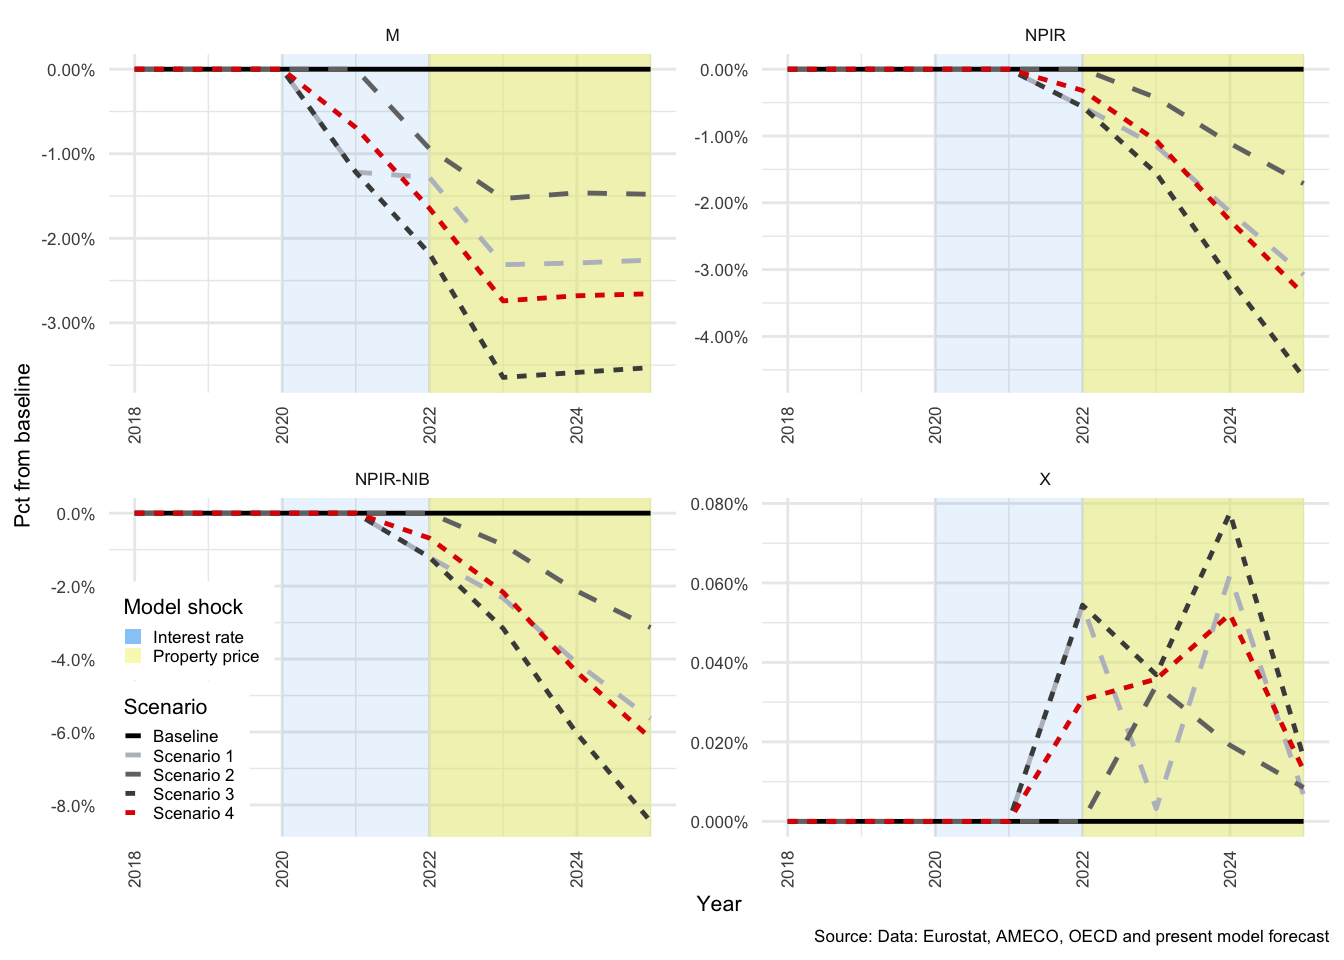
\includegraphics[width=0.95\linewidth]{figures/fl-fi-sfc-plot-row-indicators-savings-1} \caption{ROW Savings components}\label{fig:fl-fi-sfc-plot-row-indicators-savings}
\end{figure}

Imports (\(M\)) from the model are a revenue for ROW and exports (\(X\)) an expenditure. The return on net interest bearing stocks, \(r_{N_{t-1}}(NIB^W_{t-1})\), (NPIR-NIB in the plot above) depends on whether \(NIB^W\) is positive or negative.

Imports are estimated in real terms in the log-linear form in Equation (\ref{eq:imports_intext}), and depend on the level of domestic demand in the previous period, and a relative price index between domestic and foreign goods from the previous period \(\Bigg( \frac{P^y_{t-1}}{P^m_{t-1}} \Bigg)\).

\begin{equation}
ln(m_t) = \beta _i + \beta _iln \Bigg( \frac{P^y_{t-1}}{P^m_{t-1}} \Bigg) + \beta _iln(c_{t-1} + i_{t-1} + x_{t-1})
\label{eq:imports_intext}
\end{equation}

As noted by \citet{byrialsenraza2019empirical}, the ``export function is based on the
Armington (1969) model where the market share of the Danish exports is explained by
relative prices.''

This relation is captured below as annual Danish exports relative to a weighted index
of all trading partners (\(m^W_t\)), which should be determined by domestic prices
(the export price index, \(P^x_t\)) relative to foreign prices (the import price
index, \(P^m_t\)), but moderated by price elasticity (\(\beta\)).

\begin{equation}
\frac{x_t}{m^W_t} = \Bigg( \frac{P^x_t}{P^m_t}\Bigg)^ \beta
\end{equation}

Exports thus stay relatively stable in the model, and are only affected by minor changes in the relative price ratio. The lower right panel in Figure \ref{fig:fl-fi-sfc-plot-row-indicators-savings} above is a little deceptive, as the scale is very small. The most important change for ROW is a strong decline in Danish imports, which is primarily driven by the fall in HH disposable income

\hypertarget{effects-for-the-fc-sector}{%
\subsection{Effects for the FC sector}\label{effects-for-the-fc-sector}}

FC absorbs all of the imbalances in the other four sectors, and the relatively extreme shock to interest rates culminates in large changes to each. Transactions in net interest bearing assets, \(NIBTR^F\), are simply an inversion of the accumulation of \(NIBTR\) in three of the four sectors (GOV, NFC and ROW), and \(IBLTR^{F\sim H}\) is a reflection of household accumulation of deposits, \(IBATR^H\).

\begin{equation}
NIBTR^F_t = -(NIBTR^N_t + NIBTR^G_t + NIBTR^W_t )
\label{eq:nibtr_f_intext}
\end{equation}

The second, and rather indirect accumulation is that of equities to offset any equity investment by HH. The full explanation is available in the appendix, in Section \ref{sec:fi-fl-sfc-model-eq-f}. An abbreviated summary is that all other components of Equation (\ref{eq:neqtr_fc_intext}) are accounted for by accounting identities between FC and the other sectors, and the value of \(EQATR^H\) is carried into FC via \(IBLTR^{F\sim H}\). Once all other terms are netted out, the \(NEQTR^F\) value is equivalent to \(EQATR^H\). This equivalence is the redundant equation in the model, and is not specified in order to avoid over-identification.

\begin{equation}
NEQTR^F_t = NL^F_t + IBLTR^{F\sim H}_t + PENLTR^F_t - IBATR^{F\sim H}_t - NIBTR^F_t
\label{eq:neqtr_fc_intext}
\end{equation}

Because \(NIBTR^F\) captures the net flows of all other sectors, it also represents any excess or shortfall (i.e.~net lending) experienced by FC. This is because all flows of all other sectors with each other will already be captured and netted out by the sum of their \(NIBTR\) in Equation (\ref{eq:nibtr_f_intext}) above. The only unaccounted for flow is the net value of FC flows, which is captured in \(NL^F\). Again, \(NP^F\), \(I^F\)\footnote{FC investment is assumed to grow at a constant 2\% per annum.} and \(KTR^F\) are exogenous.

\begin{equation}
NL^F_t = S^F_t - I^F_t - NP^F_t + KTR^F_t
\end{equation}

Rather than show the percentage changes, Figure \ref{fig:fl-fi-sfc-plot-fc-indicators-nl} shows the actual increase in FC NL and savings as a result of the shocks in each scenario. As can be seen, the impact of the second shock is almost negligible. Scenarios 1 and 3 are almost identical, and Scenario 2 remains very close to the baseline level. It is thus the interest rate change that has the dominating effect on FC's flows and thus balance sheet. It should be unsurprising therefore that there is a substantial difference between Scenarios 3 and 4. In Scenario 4, where a greater portion of HH debt is \emph{less} sensitive to changes in interest rates, the transfer of wealth from HH to FC is substantially reduced.

\begin{figure}[H]
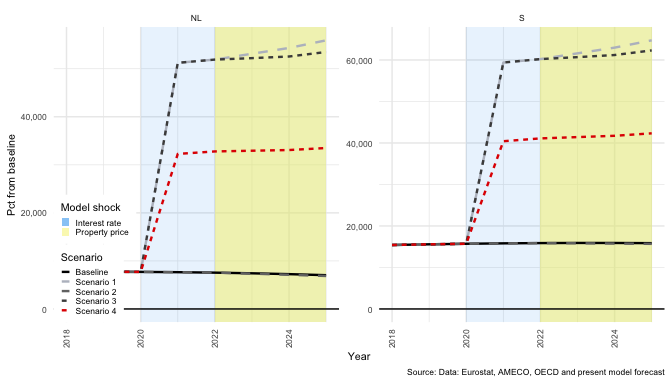
\includegraphics[width=0.95\linewidth]{figures/fl-fi-sfc-plot-fc-indicators-nl-1} \caption{FC Net Lending components}\label{fig:fl-fi-sfc-plot-fc-indicators-nl}
\end{figure}

From a very low base, \(NL^F\) rises by 569.17\%, or is roughly five and a half times larger. The shifts in the values of the underlying FC components are sensibly also substantial. Transactions in most assets are net positive, and in liabilities negative - both relative to the baseline and in absolute terms.

The exception is a decline in loan assets as HH deleverage in 2021 by -3.23\%. Apart from this single entry, HH borrowing is positive in all periods. Relative to the baseline after the first shock, \(IBLTR^{F\sim H}\) is down by -78.28\%, and \(IBATR^{F\sim H}\) is down by -73.94\%. FC is a net issuer of equity and interest bearing assets, with transactions in equity, \(NEQTR^F\), up 68.34\%, and in \(NIB\) up 61.82\%. FC thus begins to accumulate assets rapidly.

In terms of property income flows, the rise in interest rates in this example is only allowed to affect the asset returns of FC, and thus the net increase is more extreme than if we adjusted all rates of return. The total net property income received by FC, \(NPIR^F\), is 323.58\% higher. This comes from the increase in fixed and flexible rate interest receipts, which rise by 32.38\%, and 136.29\% respectively.

As noted above, FC accumulates assets rapidly. \(NEQ^F\) rises by 46.26\% and \(NIB^F\) by 2.02\%. The fall in \(IBA^{F\sim H}\) by -2.26\% and in \(IBL^{F\sim H}\) by -3.23\% almost offset each other entirely, and the final impact on net wealth of FC is an increase of 42.82\%.

Equation (\ref{eq:S_fc_intext}) highlights the income and expenditure components that contribute to FC savings, and Figure \ref{fig:fl-fi-sfc-plot-fc-indicators-saving} illustrates these components in nominal values.

\begin{equation}
\begin{split}
    S^F_t = & B2^F_t \\
            & + r^F_{A(FI)_{t-1}}(IBA^{F\sim H}_{A(FI)_{t-1}}) + r^F_{A(FL)_{t-1}}(IBA^{F\sim H}_{A(FL)_{t-1}}) \\
            & - r^F_{L_{t-1}}(IBL^{F\sim H}_{L_{t-1}}) + r_{N_{t-1}}(NIB^F_{t-1}) \\
            & + \chi _t(NEQ^F_{t-1}) -\psi _t(PENL^F_{t-1}) - T^F_t + STR^F_t - CPEN^F_t + \epsilon ^F
\end{split}
\label{eq:S_fc_intext}
\end{equation}

From Equation (\ref{eq:S_fc_intext}), \(B2^F\) and \(T^F\) are exogenous, and the change in FC output, \(Y^F\), is less than -1\%. Nominal values are illustrated here in order to give better context to the changes implied by the shocks. The percentage changes that are discussed above for Scenario 1 do not appear to be as unrealistic when viewed in these terms.

\begin{figure}
\centering
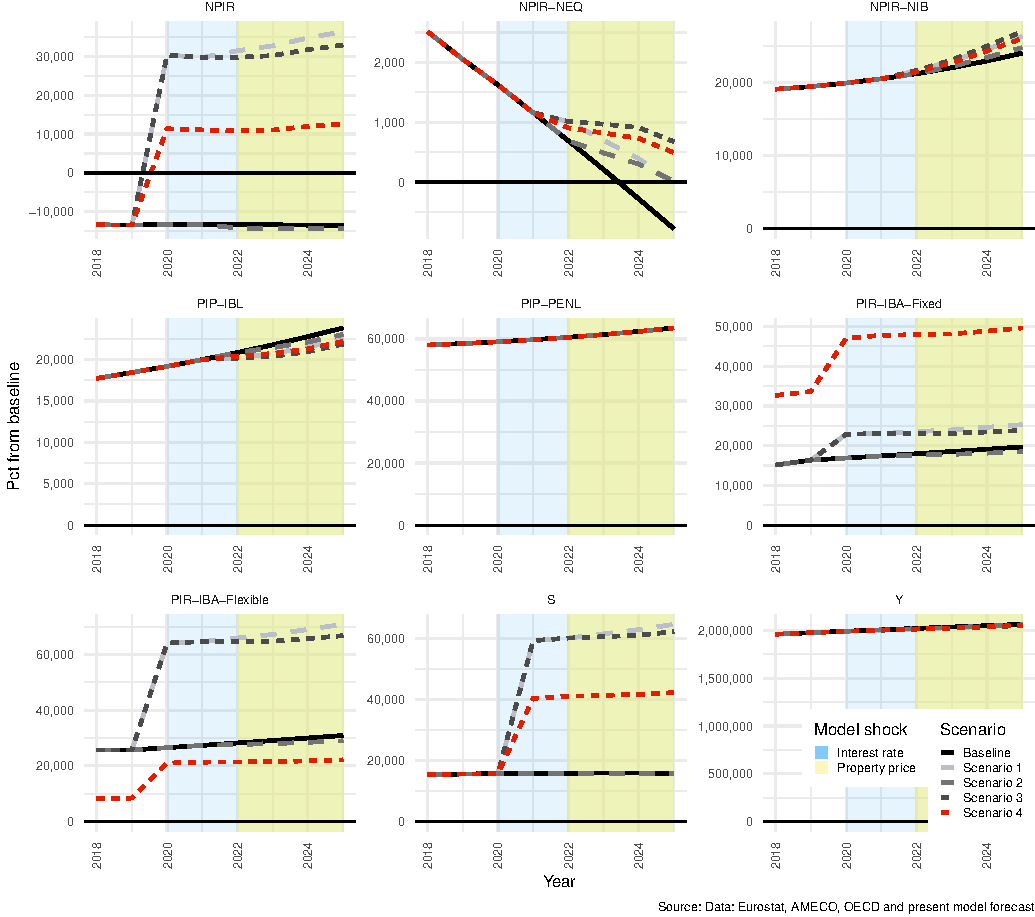
\includegraphics{figures/fl-fi-sfc-plot-fc-indicators-saving-1.pdf}
\caption{\label{fig:fl-fi-sfc-plot-fc-indicators-saving}FC Savings components}
\end{figure}

The panel titled net property income (NPIR) in the plot above is a sum of all property income flows, and is similar to Equation (\ref{eq:S_fc_intext}) above for \(S^F\), but with all other terms removed. The total impact on property income helps to identify the source of changes in FC savings. NPIR is calculated as follows.

\begin{equation}
\begin{split}
    NPIR^F_t = & + r^F_{A(FI)_{t-1}}(IBA^{F\sim H}_{A(FI)_{t-1}}) + r^F_{A(FL)_{t-1}}(IBA^{F\sim H}_{A(FL)_{t-1}}) \\
               & + r_{N_{t-1}}(NIB^F_{t-1}) + \chi _t(NEQ^F_{t-1})  \\
               & -\psi _t(PENL^F_{t-1}) - r^F_{L_{t-1}}(IBL^{F\sim H}_{L_{t-1}})
\end{split}
\label{eq:NPIR_fc_intext}
\end{equation}

The bulk of FC flows are property income paid (PIP), property income received (PIR), or NPIR. The representations in Figure \ref{fig:fl-fi-sfc-plot-fc-indicators-saving} above are categories of these property income flows. NPIR-NEQ for \(\chi _t(NEQ^F_{t-1})\) (on equities), NPIR-NIB for \(r_{N_{t-1}}(NIB^F_{t-1})\) (on net interest bearing assets with all sectors other than HH), PIR-IBA-Fixed for \(r^F_{A(FI)_{t-1}}(IBA^{F\sim H}_{A(FI)_{t-1}})\) (on fixed-rate HH debt), PIR-IBA-Flexible for \(r^F_{A(FL)_{t-1}}(IBA^{F\sim H}_{A(FL)_{t-1}})\) (on flexible-rate HH debt), PIP-IBL for \(r^F_{L_{t-1}}(IBL^{F\sim H}_{L_{t-1}})\) (on deposit liabilities).

The shock to interest rates in Scenarios 1, 3 and 4 all result in positive NPIR for FC. The substantially lower level of NPIR in Scenario 4 (the red line) can be traced back to PIR-IBA-Fixed and PIR-IBA-Flexible. The sum of the total revenue generated by the rise in interest rates is the summarised in NPIR. The steady decline of net return on equities, NPIR-NEQ, is due to the systematic issuance of equity to HH as HH demands equity. This demand is retarded slightly in all scenarios. Equity investment by HH is dependent on previous returns, previous returns on house investment and previous changes in the quantity of loans acquired. For both shock 1 and 2, it is due to the reduction in \(IBLTR^H\) and for shock 2 it is also driven by a fall in returns on houses.

The effect on FC savings, \(S^F\), is to triple the value in Scenarios 1 and 3, and double the value in Scenario 4.

\begin{figure}[H]
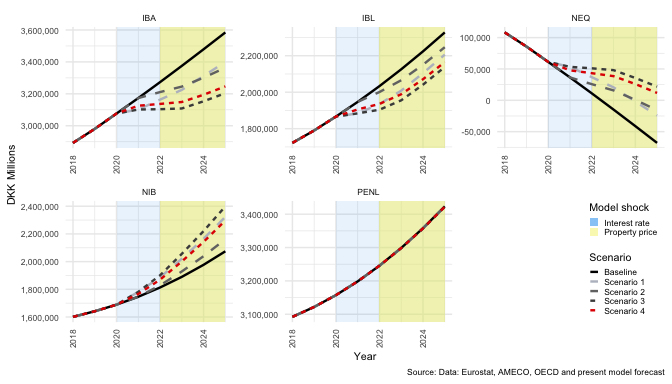
\includegraphics[width=0.95\linewidth]{figures/fl-fi-sfc-plot-FC-bs-1} \caption{FC balance sheet}\label{fig:fl-fi-sfc-plot-FC-bs}
\end{figure}

\hypertarget{sec:fi-fl-sfc-discussion}{%
\section{Discussion}\label{sec:fi-fl-sfc-discussion}}

As noted in Section \ref{sec:fi-fl-rk-dk}, many of the innovations that occurred around the world during the past decades also occurred in the Danish mortgage lending system. In addition, since the GFC, interest rates have reduced to and remained at historically low levels. These conditions provided the platform for rapid expansion of household mortgage debt leading up to the crisis, and to continued expansion of that debt in more recent years. This has coincided with the rapid recovery and inflation of asset prices. Property prices are discussed in Section \ref{sec:fi-fl-sfc-scenarios-s2} above, and as can be seen from panel (a) in Figure \ref{fig:fl-fi-sfc-plot-dk-equity-int}, Danish equity prices (the yellow line) have risen over 230\% from 2010 to 2018, with only one other European country (Latvia, the blue line) with a higher increase in its equity price index.

The main effects of the innovations that occurred were a reduction in initial payments for borrowers, a decline in the level of payments towards the outstanding principal debt (and thus a decline in the level of equity accumulation) and a significant shift of risk from investors to lenders. Danish HH responded rapidly to the innovations, and the composition of debt changed from 100\% fixed interest debt, in 2000 to less than 30\% by 2012, as can be seen in panel (b) of Figure \ref{fig:fl-fi-sfc-plot-dk-equity-int}\footnote{The gradual shift out of fixed interest bonds prior to 2003 is due to the introduction of index-linked bonds, which made up a relatively small share of less than 10\% the market, and this share reduced rapidly after 2003. There has also been a gradual move back towards more fixed-interest rate products since 2012.}.

\begin{figure}[H]
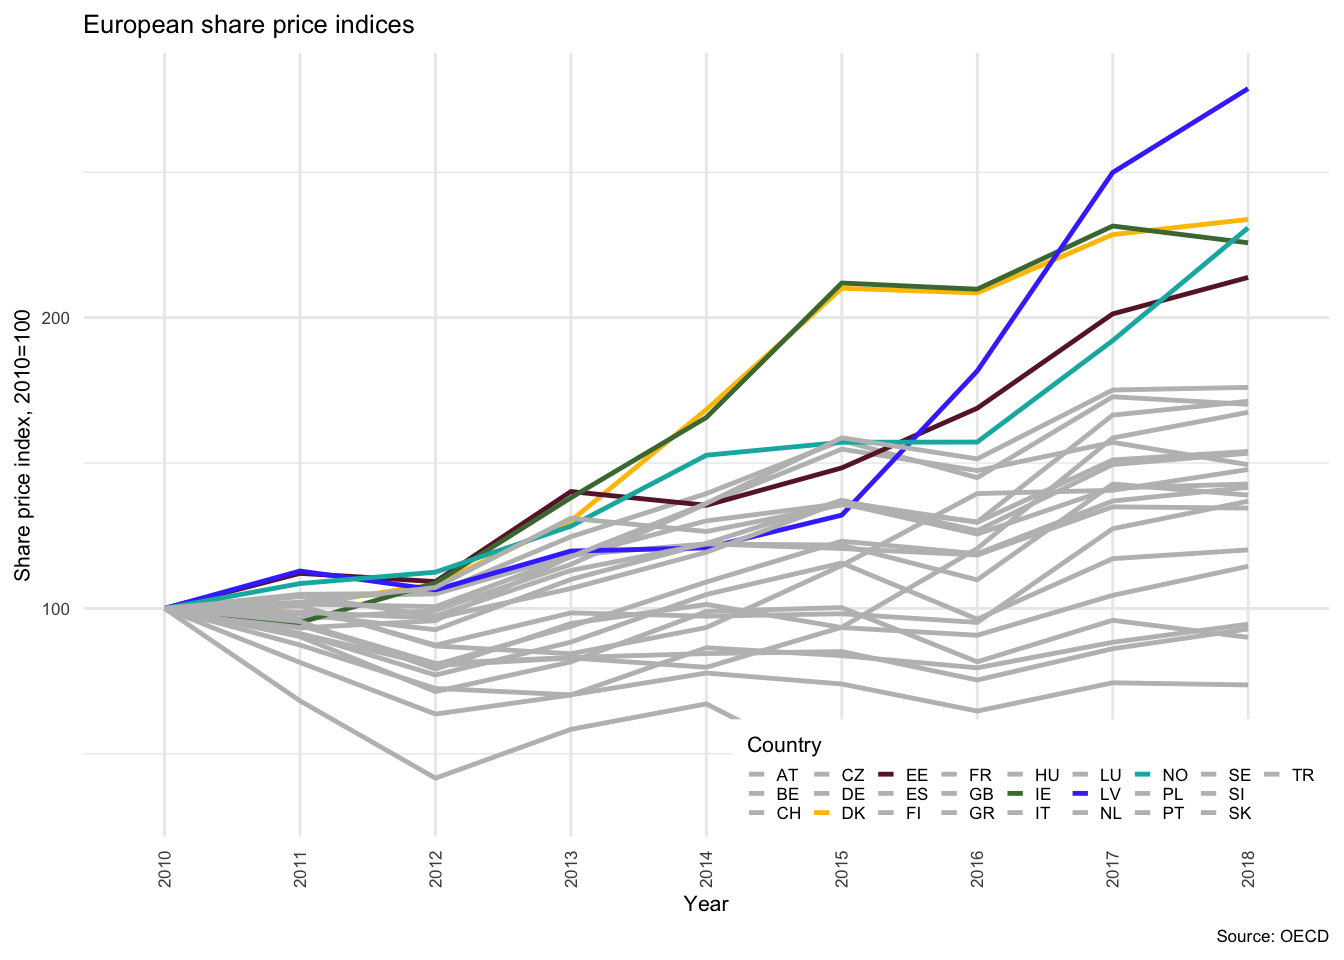
\includegraphics[width=0.95\linewidth]{figures/fl-fi-sfc-plot-dk-equity-int-1} 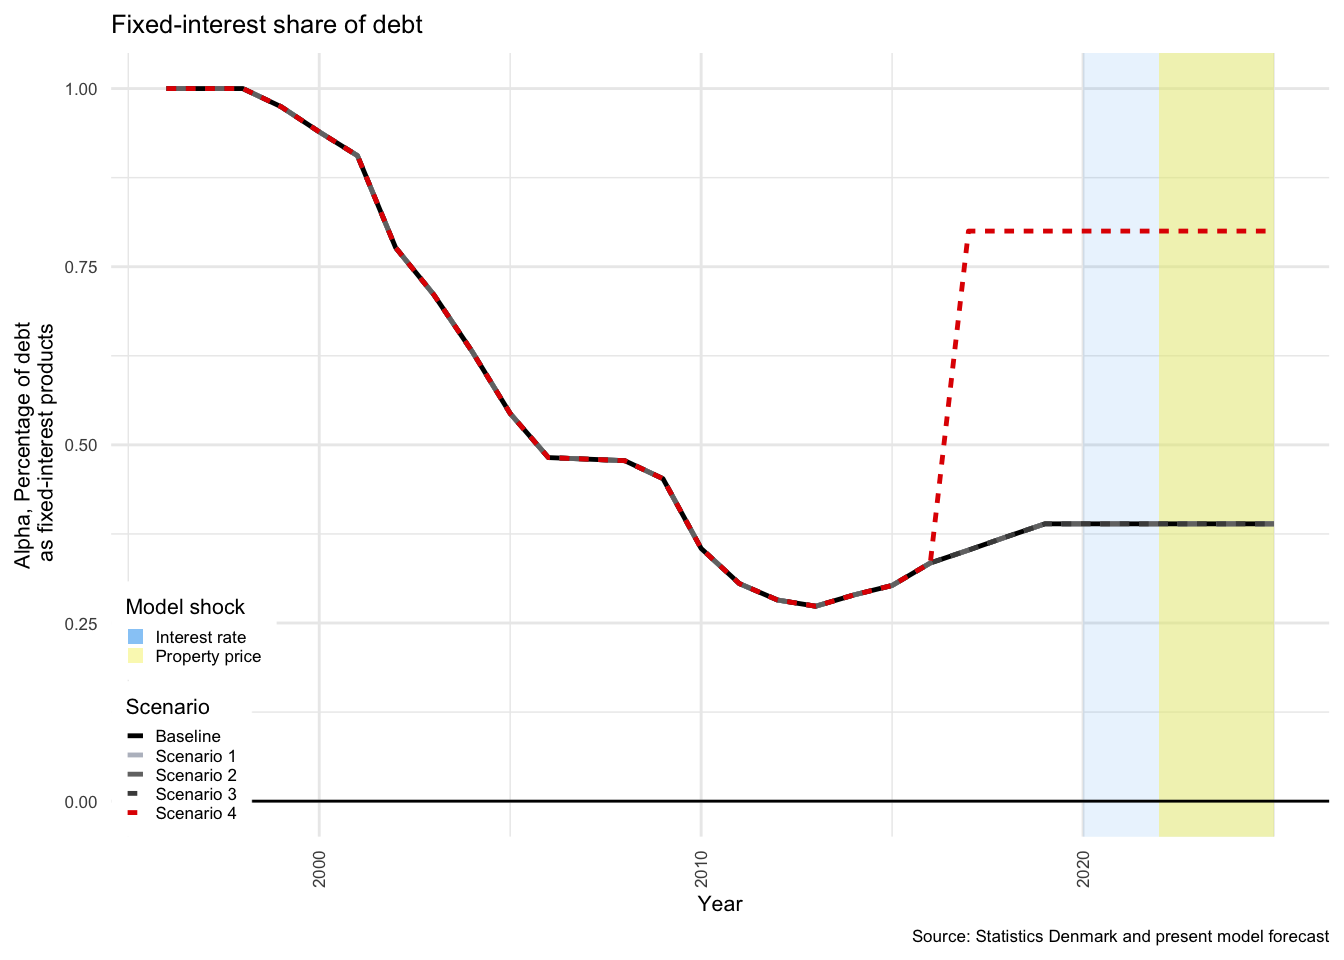
\includegraphics[width=0.95\linewidth]{figures/fl-fi-sfc-plot-dk-equity-int-2} \caption{Share prices and mortgage composition}\label{fig:fl-fi-sfc-plot-dk-equity-int}
\end{figure}

The major benefits of fixed interest products include stability of expenditures, insulation against unforseen interest rate hikes, and the possibility to refinance at various favourable instances (stemming from the buy-back, and prepayment rights assigned to borrowers \citep{Skinhoj2019}). Flexible interest rate products on the other hand, provide low initial cost of borrowing, but transfer interest rate risk to the borrower. Revisions to the coupon rate on the counter-balancing bonds also create a significant opportunity cost for ARM borrowers if rates rise. This is opportunity cost is enhanced if it is a distressed borrower, or the borrower faces negative shocks, such as a loss of income or an injury. A fixed rate borrower (even without amortization) would be able to accept a lower sale value for their property, since the bond that represents the outstanding debt would reprice downwards as interest rates rise. In the case of an interest rate increase, flexible rate borrowers face the same possibility of unfavourable property market conditions, but the price of bonds outstanding will remain relatively constant, due to the re-setting of the short-term fixation of coupon payments. Flexible rate borrowers, and borrowers with interest-only periods thus face a much higher risk of falling into negative equity if house prices fall.

Many of these dynamics are captured in the model presented in this article, as are several economic relationships between the real and financial sides of the economy. These connections make it possible to show some of the expected ``real'' economic feedback effects of each shock. Although it is a highly simplified version of the Danish mortgage market, it is still able to provide a realistic scale for the core transmission channels for each of the shocks, and due to the simple structure of the model, it was relatively easy to incorporate a split in the composition of debt of HH.

One of the goals at the outset was to test the sensitivity of HH balance sheets for different compositions of debt. Two shocks were introduced across four scenarios. The primary effect of the first shock, an increase in interest rates by 2\% in 2020, was an immediate reduction in HH income. The primary effect of the second shock, a decline in property prices by 20\% in 2022, was to reduce the level of HH capital and the attractiveness of housing as an investment alternative. These two shocks were then compounded in Scenarios 3 and 4, but in Scenario 4 the level of debt held in fixed-interest products (\(\alpha\)) was increased from around 37\% to 80\%, as shown in panel (b) of Figure \ref{fig:fl-fi-sfc-plot-dk-equity-int} above.

The model behaved as expected, and in Scenario 3, with the higher proportion of ARMs, HH are exposed to significantly greater income volatility than in Scenario 4, a result that is corroborated by \citet{DanmarksNationalbank2016a} and \citet{Skinhoj2019}. This transmits to both the real and financial sides of the economy, with lower economic output and higher unemployment as a result of the increased sensitivity. The results in Section \ref{sec:fi-fl-sfc-simulations} above suggest that for a significant rise in interest rates, or a collapse in property prices, HH would be in a more favourable financial position as a sector if the proportion of mortgage debt held in fixed-interest products (\(\alpha\)) was higher. This suggests that policies with a focus on increasing the coverage of fixed-interest-rate products in the mortgage financing system would result in a more resilient HH, and economy as a whole.

The specific movements of variables, however, should be interpreted with caution, as the shocks in this model are not designed to provide a comprehensive economic response within the model structure. Especially since it is only the rates that affect the cost of borrowing that are adjusted in shock 1.

In terms of the transmission channels in the model, HH is a key driver. The primary transmission channel in the interest rate shock is the credit channel, and it is clearly more impactful where interest rates are more sensitive. In a more realistic setting, the rise in interest rates would also affect HH incomes positively. In Denmark, pension funds hold a large portion of the outstanding covered covered bonds on behalf of households, and fees of the mortgage lending companies are generally a fixed rate. This would mean that increased mortgage costs should translate directly to increased pension incomes. HH pension assets are also substantially larger than HH debt, which means that if an interest rate hike resulted in a rise of the rates of return on most asset classes, then HH could experience a net gain. One argument against this is that pension assets are not directly accessible, and therefore would not contribute to short term disposable income of HH. HH in this case do not have discretion over the consumption of all wealth, and therefore those parts that are inaccessible should be excluded.

The current form of the model is also important to consider. Presently, HH consume out of wealth, and there is a positive return on \(IBA\), which are assumed to be deposits. If we adjust the rate of return on \(IBA\) (\(r^H_N\)) upwards, it would change relative rates of return available for HH investment allocation, and would lead to a rapid accumulation of \(IBA\). It would also drive a large positive effect on HH income, which would conceal the negative effects to disposable income that are displayed in the current form. This would, at least in the short run, not be in line with realistic expectations regarding accessible disposable income of HH.

Even if other asset class returns are adjusted to mitigate the fall in HH disposable income, investment will necessarily be lower as the cost of borrowing rises. In the case of an interest rate rise, aggregate demand and output would still decline, pushing unemployment upwards and providing downward pressure on the wage rate. after several years, the relative improvement in competitiveness in export prices would have a positive influence on exports and negative on imports. Ultimately this would strengthen the current account balance, but at the expense of higher unemployment in the domestic economy. The positive feedback of rising imports on wage income and output would depend on the elasticities of wages to changes in output, and imports and exports to relative price changes. The effect of a fall in house prices on housing investment would also remain in the short-term, as it is dependent on previous returns.

Another transmission channel that would be concealed is the negative pressure that a fall in demand has on the tax base, and therefore on GOV revenues. In the analysis above, it is clear that the fall in overall demand would lead to a fall in employment, a fall in tax revenues and therefore a large negative shift in the GOV net financing requirement. If the Danish GOV enforces a balanced budget, there would need to be a reduction in GOV spending, and the vast majority of this spending is split between a tax funded pension scheme, healthcare, disability support, family and child support. A reduction in any of these categories would result in a further reduction of output and ultimately in HH income.

Even with the simplifications, it should be safe to conclude that larger portions of debt in fixed-interest products would result in much lower volatility of HH disposable income. The use of a more comprehensive model, rather than a simple test of income volatility, allows us to observe the expected accumulation effects of the two shocks for different levels of \(\alpha\). The exogeneity of asset prices and rates of return are potential drawbacks, however, it is not obvious that creating endogenous links between financial markets, assets and rates of return (i.e.~a more integrated financial sector) would be an improvement on the current model structure. At present, the most immediate transmission channels for each of the shocks are transparent, and because of the empirical nature of the model, it is possible to get an accurate scale of the initial effects of the shocks, without the complication of complex interdependencies between markets. There is a clear trade-off between complexity with greater accuracy, and better interpretability with greater transparency.

The more complete macroeconomic SFC model presented above requires attention to the gross levels of economic stocks and flows, and thus makes it possible to identify that the rise in HH \(NL\) following the second shock (the fall in property prices) was not due to positive changes in HH. Contrarily, HH experienced a decline in investment demand, together with rising unemployment. The model presented here helps to prevent such misinterpretations, and to provide a more complete picture of the possible impact of shocks\footnote{In addition to the alterations made, the output of the model is presented in an alternative format. The tables in the appendix provide an exhaustive list of all elements applicable to each sector that are affected by each shock. This cross-section provides at least two things to the modeller. Firstly it identifies the components applicable to each sector that are most dramatically impacted. Secondly, the comprehensive list of affected components expand as a shock propagates through the economy and assists in the identification of timing errors in the model structure.}.

The model unfortunately does not presently incorporate some key issues from the mortgage system, including the effect of changes in loan-to-value (LTV) ratios, or second round credit risk effects that might occur due to loss of income due to unemployment. The inclusion of a measure of non-performing loans or some other measure of credit risk might be able to capture these effects. Perhaps the most relevant omission, for the present discussion, is the effect of refinancing behaviour on the composition of debt, although this is not a simple matter to include, as noted by \citet[pp.~19]{Skinhoj2019}, ``The stochastic modelling of prepayment behaviour is a complex task and is outside the scope for most international investors.''

The possibility to explore a variety of modifications and alterations is also one of the major benefits that the baseline version of the model offers. It has made it possible to explore some of the complex economic feedback mechanisms described above. This version is also under continuous development by the MaMTEP group\footnote{The Macroeconomic Methodology, Theory and Economic Policy Research Group, Aalborg University.}, and as additional economic components are explored in greater detail it will be possible to include any alterations that strengthen the core structure.

\hypertarget{sec:fi-fl-sfc-conclusion}{%
\section{Conclusion}\label{sec:fi-fl-sfc-conclusion}}

The Danish mortgage financing system has experienced several innovations in recent decades. Collectively these innovations have had a variety of benefits for borrowers, but these come with a transfer of responsibility and risk to the borrower. One of the most prominent innovations was the introduction of adjustable rate mortgages (ARMs) with periods of interest fixation of a variety of lengths.

Access to individual level administrative data-sets allowed for the construction of aggregate outstanding mortgage data from 2009 to 2017, and highlights the increased concentration of flexible-rate mortgage debt. By the end of 2017, after the introduction of ARM products, approximately 63\% of all mortgage debt outstanding was subject to an interest rate adjustment within 5 years. These products were collectively considered to be flexible-interest rate products in the analysis above, and the remaining debt considered to be fixed rate.

The model in this article was adapted from \citet{byrialsenraza2019empirical} to explore the effects of this shift on the stability of incomes and balance sheets of the Danish economy. The primary innovation in the model was to introduce the split in debt, and to test the effect of the changes on the overall sensitivity of incomes and balance sheets, with a particular focus on HH. There are some additional changes that could be incorporated in future versions of the model that might strengthen the outputs of the model. Firstly, additional data could be sourced to provide a further split in HH debt between mortgage institute, bank and consumer debt. Secondly, it might be possible to actively model the refinancing behaviour of Danish property buyers\footnote{There is unfortunately no data available at an individual level that would be representative of a rising interest rate environment.}. It might also be possible to include some measure of credit supply constraints, and or borrower risk, for example, non-performing loans. Further developments of the model could make this possible.

The core aim of the analysis was to test the sensitivity of HH and economic conditions of a potential shift in the composition of debt from ARM type products to fixed-interest products. This is an intuitively simple proposition, but the accurately scaled empirical model presented in this article provides a clear indication of the potential scale of these impacts. For a shift in the fixed proportion from 37\% up to 80\%, in the case of a 2\% point increase in interest rates and a 20\% decline in property prices, the difference in aggregate unemployment effects could be as much as 2\%. The effects discussed for each sector mirror this increase in sensitivity. Both in the initial effects and in terms of volatility in subsequent periods.

The results thus provide evidence to support reports made by the IMF \citep{sheehy2014}, the Danish national bank \citep{DanmarksNationalbank2016a} and the leading mortgage credit institution in Denmark, Nykredit Realkredit \citep{Skinhoj2019}, that the increased concentration of household debt in ARM (flexible-rate) products has resulted in greater sensitivity (and thus less stability) of both HH and the Danish economy in general. This does not imply that the level of outstanding debt poses a systemic economic risk. Again in support of reports presented by the above institutions, it should be noted that simultaneous and sizable shocks to both the cost of borrowing and to property prices only resulted in modest effects on overall output, even where the shock is restricted to borrowing costs.

In contrast to suggestions regarding the systemic risk of household debt in itself, the analysis suggests that the potential risks related to the present high ratio of HH debt to disposable income in Denmark can be dramatically reduced through a migration of HH mortgage debt away from ARM type products towards fixed interest rate products. The all-time low levels of interest rates that are currently available also present an excellent opportunity to support this transition.

\hypertarget{sec:Appendix}{%
\section{Appendix}\label{sec:Appendix}}

\hypertarget{sec:fi-fl-sfc-Ap-A-MtoL}{%
\subsection{Mortgage debt as a percentage of total loans to non-financial private sector (nominal, local currency)}\label{sec:fi-fl-sfc-Ap-A-MtoL}}

\begin{figure}
\centering
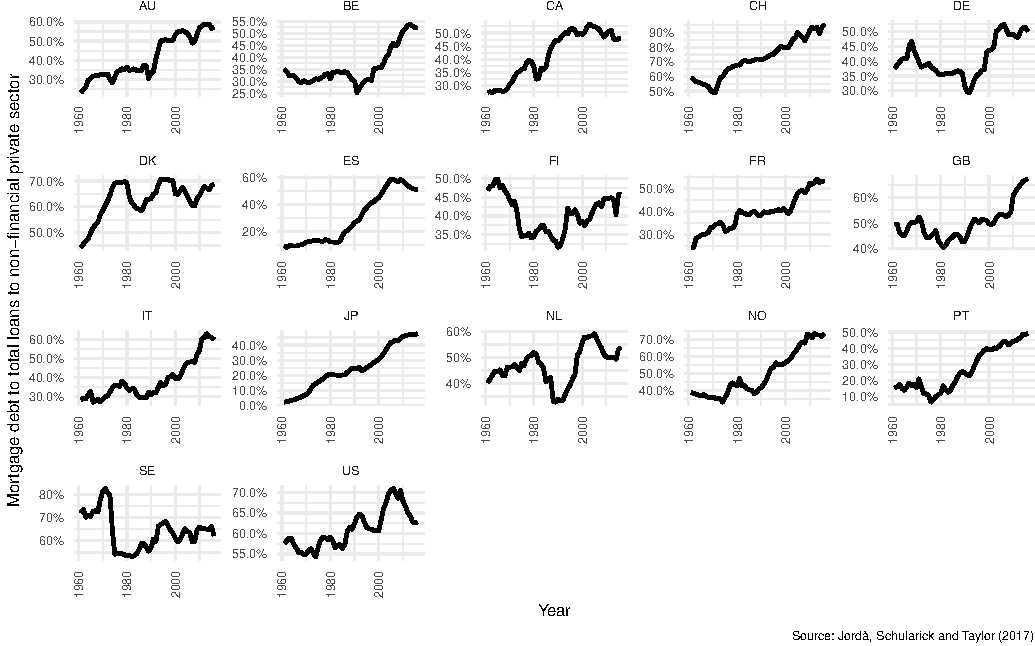
\includegraphics{figures/fl-fi-sfc-lt-debt-1.pdf}
\caption{\label{fig:fl-fi-sfc-lt-debt}Mortgage debt as percentage of total loans}
\end{figure}

\hypertarget{sec:fi-fl-sfc-Ap-A-MtoGDP}{%
\subsection{Mortgage debt to GDP}\label{sec:fi-fl-sfc-Ap-A-MtoGDP}}

\begin{figure}
\centering
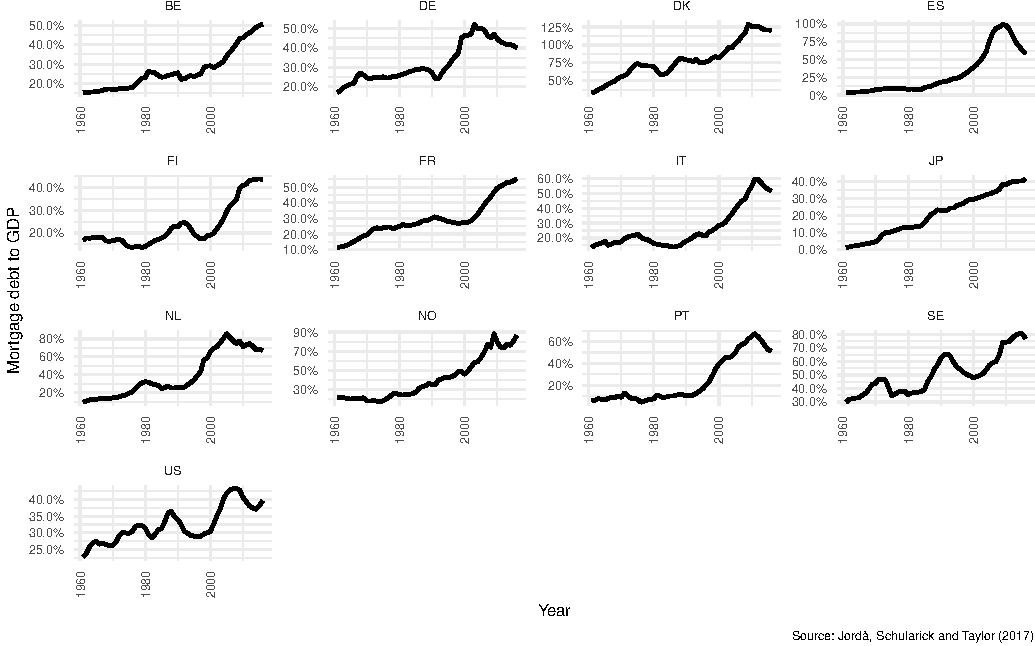
\includegraphics{figures/fl-fi-sfc-hh-debt-1.pdf}
\caption{\label{fig:fl-fi-sfc-hh-debt}Mortgage debt to GDP}
\end{figure}

\hypertarget{sec:fi-fl-sfc-Ap-A-OECD-house-prices}{%
\subsection{House Prices}\label{sec:fi-fl-sfc-Ap-A-OECD-house-prices}}

\begin{table}

\caption{\label{tab:oecd-house-price-table}OECD House price index changes, Year on year}
\centering
\begin{tabular}[t]{l|l|l|l}
\hline
Country & 2000 to 2007 & 2007 to 2009 & 2009 to 2018\\
\hline
Estonia & 15.89\textbackslash{}\% & -17.06\textbackslash{}\% & 11.33\textbackslash{}\%\\
\hline
Costa Rica & 08.94\textbackslash{}\% & 06.07\textbackslash{}\% & 04.11\textbackslash{}\%\\
\hline
Austria & 03.63\textbackslash{}\% & 03.01\textbackslash{}\% & 03.97\textbackslash{}\%\\
\hline
Colombia & 04.58\textbackslash{}\% & 04.79\textbackslash{}\% & 03.85\textbackslash{}\%\\
\hline
Hungary & 13.52\textbackslash{}\% & 08.14\textbackslash{}\% & 03.01\textbackslash{}\%\\
\hline
Czech Republic & 05.25\textbackslash{}\% & 16.46\textbackslash{}\% & 02.83\textbackslash{}\%\\
\hline
United States & 04.10\textbackslash{}\% & 01.82\textbackslash{}\% & 02.78\textbackslash{}\%\\
\hline
Netherlands & 03.35\textbackslash{}\% & 02.03\textbackslash{}\% & 02.62\textbackslash{}\%\\
\hline
Ireland & 16.65\textbackslash{}\% & -12.57\textbackslash{}\% & 02.50\textbackslash{}\%\\
\hline
Finland & 02.96\textbackslash{}\% & 00.33\textbackslash{}\% & 02.43\textbackslash{}\%\\
\hline
Israel & 00.55\textbackslash{}\% & 05.02\textbackslash{}\% & 02.40\textbackslash{}\%\\
\hline
Korea, Republic of & 03.01\textbackslash{}\% & 01.93\textbackslash{}\% & 02.39\textbackslash{}\%\\
\hline
Norway & 03.72\textbackslash{}\% & 03.27\textbackslash{}\% & 02.35\textbackslash{}\%\\
\hline
Poland & 08.40\textbackslash{}\% & 05.06\textbackslash{}\% & 02.23\textbackslash{}\%\\
\hline
Mexico & 06.03\textbackslash{}\% & 03.23\textbackslash{}\% & 02.15\textbackslash{}\%\\
\hline
New Zealand & 00.97\textbackslash{}\% & 02.29\textbackslash{}\% & 02.07\textbackslash{}\%\\
\hline
Denmark & 03.11\textbackslash{}\% & 02.95\textbackslash{}\% & 01.98\textbackslash{}\%\\
\hline
United Kingdom & 03.52\textbackslash{}\% & 02.65\textbackslash{}\% & 01.95\textbackslash{}\%\\
\hline
Portugal & 03.37\textbackslash{}\% & 02.90\textbackslash{}\% & 01.76\textbackslash{}\%\\
\hline
Sweden & 02.56\textbackslash{}\% & 02.92\textbackslash{}\% & 01.56\textbackslash{}\%\\
\hline
Latvia & 11.22\textbackslash{}\% & 03.58\textbackslash{}\% & 01.39\textbackslash{}\%\\
\hline
Luxembourg & 02.87\textbackslash{}\% & 02.79\textbackslash{}\% & 01.31\textbackslash{}\%\\
\hline
Germany & 01.30\textbackslash{}\% & 01.17\textbackslash{}\% & 01.23\textbackslash{}\%\\
\hline
Canada & 01.64\textbackslash{}\% & 01.63\textbackslash{}\% & 01.09\textbackslash{}\%\\
\hline
Slovenia & 12.31\textbackslash{}\% & 02.53\textbackslash{}\% & 01.00\textbackslash{}\%\\
\hline
France & 03.36\textbackslash{}\% & 02.15\textbackslash{}\% & 00.82\textbackslash{}\%\\
\hline
Italy & 03.07\textbackslash{}\% & 02.95\textbackslash{}\% & 00.80\textbackslash{}\%\\
\hline
Switzerland & 01.87\textbackslash{}\% & 02.46\textbackslash{}\% & 00.75\textbackslash{}\%\\
\hline
Slovakia & 22.41\textbackslash{}\% & 04.09\textbackslash{}\% & 00.42\textbackslash{}\%\\
\hline
Spain & 05.69\textbackslash{}\% & 03.72\textbackslash{}\% & 00.29\textbackslash{}\%\\
\hline
Greece & 06.25\textbackslash{}\% & 03.82\textbackslash{}\% & -2.33\textbackslash{}\%\\
\hline
Japan & -0.27\textbackslash{}\% & -0.22\textbackslash{}\% & -0.31\textbackslash{}\%\\
\hline
\end{tabular}
\end{table}

\begin{figure}
\centering
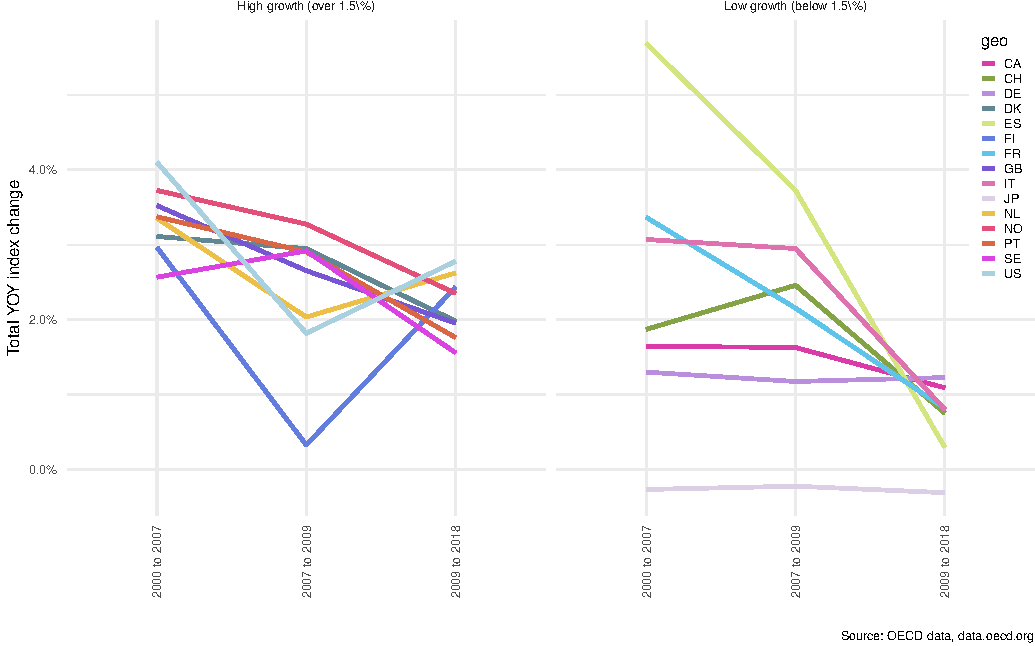
\includegraphics{figures/oecd-house-prices-1.pdf}
\caption{\label{fig:oecd-house-prices}OECD house prices: Year-on-year changes}
\end{figure}

\begin{figure}
\centering
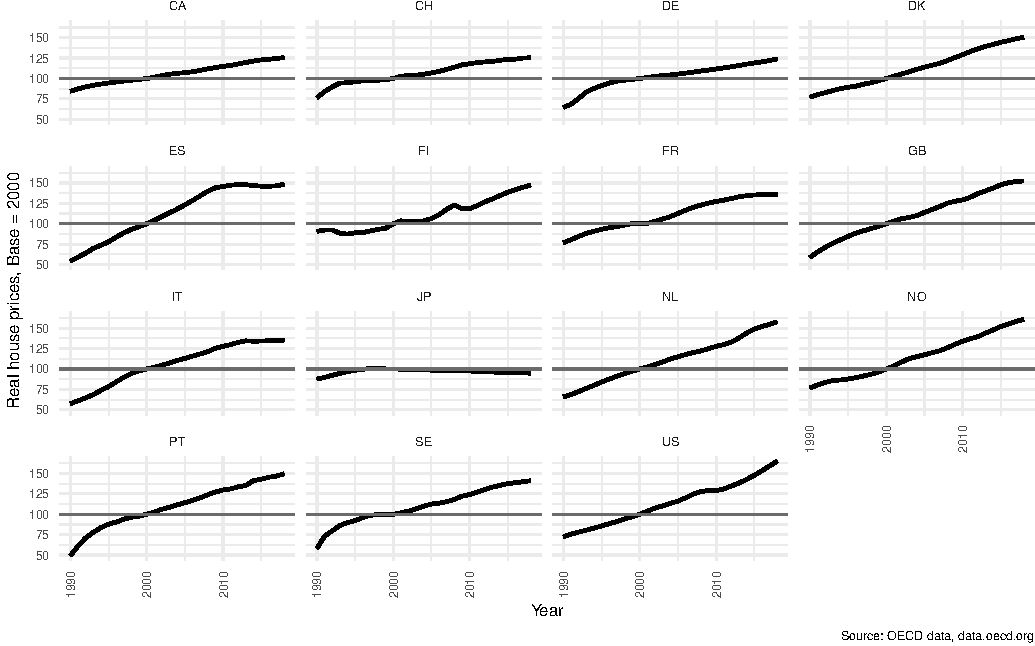
\includegraphics{figures/oecd-house-prices-facet-1.pdf}
\caption{\label{fig:oecd-house-prices-facet}OECD house prices: Real price index}
\end{figure}

\hypertarget{sec:fi-fl-sfc-Ap-A-scenario-summaries}{%
\subsection{Simulation most affected variables in each shock}\label{sec:fi-fl-sfc-Ap-A-scenario-summaries}}

\hypertarget{scenario-1-percentage-from-baseline-an-increase-in-2020-interest-rates-measured-in-2021}{%
\subsubsection{Scenario 1: Percentage from baseline: An increase in 2020 interest rates, measured in 2021}\label{scenario-1-percentage-from-baseline-an-increase-in-2020-interest-rates-measured-in-2021}}

\begin{table}

\caption{\label{tab:most-affected-scenario-1-perc-2020-economy}Most affected variables: Perc change from baseline: Scenario 1, 2021: Economy wide}
\centering
\fontsize{10}{12}\selectfont
\begin{tabular}[t]{l|l|l|l}
\hline
Variables & Type & Description & Change\\
\hline
PY & Deflation index & Price deflator: GDP & 00.0082\textbackslash{}\%\\
\hline
CAB & Flow & Current account balance & 10.9700\textbackslash{}\%\\
\hline
FAB & Flow & Financial account balance & -10.9700\textbackslash{}\%\\
\hline
NX & Flow & Net Exports & 10.5161\textbackslash{}\%\\
\hline
I-Real prices & Flow & Gross fixed capital formation & -1.2468\textbackslash{}\%\\
\hline
I & Flow & Gross fixed capital formation & -1.2468\textbackslash{}\%\\
\hline
M & Flow & Imports & -1.2173\textbackslash{}\%\\
\hline
M-Real prices & Flow & Imports & -1.2173\textbackslash{}\%\\
\hline
PRIVATE & Flow & Gross income & -0.6908\textbackslash{}\%\\
\hline
S-Real prices & Flow & Savings & -0.5725\textbackslash{}\%\\
\hline
S & Flow & Savings & -0.5638\textbackslash{}\%\\
\hline
Y-Real prices & Flow & Total income & -0.2097\textbackslash{}\%\\
\hline
Y & Flow & Total income & -0.2016\textbackslash{}\%\\
\hline
B2 & Flow & Gross operating surplus & -0.1126\textbackslash{}\%\\
\hline
ULC & Rate & Labour force: Unit labour cost: Price index: Index for the price deflator with reference to 2010 (all other price deflator indices are referenced to 2010) & 00.2021\textbackslash{}\%\\
\hline
UL-COST & Rate & Labour force: Unit labour cost & 00.2020\textbackslash{}\%\\
\hline
CU & Ratio & Capacity Utilisation (Real GNI  /  real capital stock) & -0.2098\textbackslash{}\%\\
\hline
WS & Ratio & Wage share & 00.0442\textbackslash{}\%\\
\hline
\end{tabular}
\end{table}

\begin{table}

\caption{\label{tab:most-affected-scenario-1-perc-2020-HH}Most affected variables: Perc change from baseline: Scenario 1, 2021: HH}
\centering
\fontsize{10}{12}\selectfont
\begin{tabular}[t]{l|l|l|l}
\hline
Variables & Type & Description & Change\\
\hline
PIP-IBL-HH-Flexible & Flow & Property income paid: IBL & 136.2914\textbackslash{}\%\\
\hline
PIP-IBL-HH & Flow & Property income paid: IBL & 95.8530\textbackslash{}\%\\
\hline
IBA-HH-Transactions & Flow & Financial Assets: Interest bearing assets & -78.2793\textbackslash{}\%\\
\hline
FL-HH-Transactions & Flow & Financial liabilities & -73.9372\textbackslash{}\%\\
\hline
IBL-HH-Transactions & Flow & Financial Liabilities: Interest bearing liabilities & -73.9372\textbackslash{}\%\\
\hline
EQA-HH-Transactions & Flow & Financial Assets: Equity assets & -68.3376\textbackslash{}\%\\
\hline
NPIR-HH & Flow & Net property income received: Total & -58.6600\textbackslash{}\%\\
\hline
FA-HH-Transactions & Flow & Financial Assets & -54.5574\textbackslash{}\%\\
\hline
PIP-IBL-HH-Fixed & Flow & Property income paid: IBL & 32.3802\textbackslash{}\%\\
\hline
FNL-HH & Flow & Financial Net Lending (Balance) & -16.6354\textbackslash{}\%\\
\hline
NL-HH & Flow & Sector Balance & -16.6354\textbackslash{}\%\\
\hline
S-HH & Flow & Savings & -10.3028\textbackslash{}\%\\
\hline
INV-HH-Real prices & Flow & Gross fixed capital formation & -6.8066\textbackslash{}\%\\
\hline
INV-HH & Flow & Gross fixed capital formation & -6.8066\textbackslash{}\%\\
\hline
PIR-IBA-HH & Flow & Property income received: IBA & -3.2347\textbackslash{}\%\\
\hline
Y-D-HH & Flow & Disposable Income & -2.5806\textbackslash{}\%\\
\hline
Y-HH & Flow & Total income & -2.5806\textbackslash{}\%\\
\hline
TAX-HH & Flow & Tax & -2.5806\textbackslash{}\%\\
\hline
Y-D-HH-Real prices & Flow & Disposable Income & -2.5806\textbackslash{}\%\\
\hline
C-HH-Real prices & Flow & Consumption & -1.3327\textbackslash{}\%\\
\hline
C-HH & Flow & Consumption & -1.3326\textbackslash{}\%\\
\hline
R-IBL-HH-Flexible & Rate & Rate of interest: Interest bearing liabilities & 141.7474\textbackslash{}\%\\
\hline
R-IBL-HH-Fixed & Rate & Rate of interest: Interest bearing liabilities & 35.4369\textbackslash{}\%\\
\hline
IBA-HH & Stock & Financial Assets: Interest bearing assets & -3.2347\textbackslash{}\%\\
\hline
IBL-HH & Stock & Financial Liabilities: Interest bearing liabilities & -2.2569\textbackslash{}\%\\
\hline
IBL-HH-Fixed & Stock & Financial Liabilities: Interest bearing liabilities & -2.2569\textbackslash{}\%\\
\hline
IBL-HH-Flexible & Stock & Financial Liabilities: Interest bearing liabilities & -2.2569\textbackslash{}\%\\
\hline
FA-HH & Stock & Financial Assets & -1.1087\textbackslash{}\%\\
\hline
EQA-HH & Stock & Financial Assets: Equity assets & -0.8157\textbackslash{}\%\\
\hline
K-HH & Stock & Stock of Capital & -0.2520\textbackslash{}\%\\
\hline
K-HH-Real prices & Stock & Stock of Capital & -0.2520\textbackslash{}\%\\
\hline
NW-HH & Stock & Net Wealth & -0.2223\textbackslash{}\%\\
\hline
NW-HH-Real prices & Stock & Net Wealth & -0.2222\textbackslash{}\%\\
\hline
FNW-HH-Real prices & Stock & Financial net wealth & -0.2044\textbackslash{}\%\\
\hline
FNW-HH & Stock & Financial net wealth & -0.2044\textbackslash{}\%\\
\hline
\end{tabular}
\end{table}

\vspace{1cm}
\begin{table}

\caption{\label{tab:most-affected-scenario-1-perc-2020-NFC}Most affected variables: Perc change from baseline: Scenario 1, 2021: NFC}
\centering
\fontsize{10}{12}\selectfont
\begin{tabular}[t]{l|l|l|l}
\hline
Variables & Type & Description & Change\\
\hline
FNL-NFC & Flow & Financial Net Lending (Balance) & -12.6166\textbackslash{}\%\\
\hline
NIB-NFC-Transactions & Flow & Net financial stock: Interest bearing & -12.6166\textbackslash{}\%\\
\hline
NL-NFC & Flow & Sector Balance & -12.6166\textbackslash{}\%\\
\hline
S-NFC & Flow & Savings & -1.1026\textbackslash{}\%\\
\hline
TAX-NFC & Flow & Tax & -0.2016\textbackslash{}\%\\
\hline
B2-NFC & Flow & Gross operating surplus & -0.1858\textbackslash{}\%\\
\hline
NIB-NFC & Stock & Net financial stock: Interest bearing & -0.5636\textbackslash{}\%\\
\hline
NW-NFC & Stock & Net Wealth & -0.2341\textbackslash{}\%\\
\hline
FNW-NFC & Stock & Financial net wealth & -0.2042\textbackslash{}\%\\
\hline
\end{tabular}
\end{table}

\begin{table}

\caption{\label{tab:most-affected-scenario-1-perc-2020-FC}Most affected variables: Perc change from baseline: Scenario 1, 2021: FC}
\centering
\fontsize{10}{12}\selectfont
\begin{tabular}[t]{l|l|l|l}
\hline
Variables & Type & Description & Change\\
\hline
FNL-FC & Flow & Financial Net Lending (Balance) & 569.1674\textbackslash{}\%\\
\hline
NL-FC & Flow & Sector Balance & 569.1674\textbackslash{}\%\\
\hline
NPIR-FC & Flow & Net property income received: Total & 323.5769\textbackslash{}\%\\
\hline
S-FC & Flow & Savings & 275.5754\textbackslash{}\%\\
\hline
PIR-IBA-FC-HH-Flexible & Flow & Property income received: IBA & 136.2914\textbackslash{}\%\\
\hline
IBL-FC-HH-Transactions & Flow & Financial Liabilities: Interest bearing liabilities & -78.2793\textbackslash{}\%\\
\hline
IBA-FC-HH-Transactions & Flow & Financial Assets: Interest bearing assets & -73.9372\textbackslash{}\%\\
\hline
NEQ-FC-Transactions & Flow & Net financial stock: Equity & 68.3376\textbackslash{}\%\\
\hline
NIB-FC-Transactions & Flow & Net financial stock: Interest bearing & 61.8225\textbackslash{}\%\\
\hline
PIR-IBA-FC-HH-Fixed & Flow & Property income received: IBA & 32.3802\textbackslash{}\%\\
\hline
Y-FC & Flow & Total income & -0.0442\textbackslash{}\%\\
\hline
NEQ-FC & Stock & Net financial stock: Equity & 46.2640\textbackslash{}\%\\
\hline
NW-FC & Stock & Net Wealth & 42.8191\textbackslash{}\%\\
\hline
FNW-FC & Stock & Financial net wealth & 23.0242\textbackslash{}\%\\
\hline
IBL-FC-HH & Stock & Financial Liabilities: Interest bearing liabilities & -3.2347\textbackslash{}\%\\
\hline
IBA-FC-HH & Stock & Financial Assets: Interest bearing assets & -2.2569\textbackslash{}\%\\
\hline
NIB-FC & Stock & Net financial stock: Interest bearing & 02.0236\textbackslash{}\%\\
\hline
\end{tabular}
\end{table}

\begin{table}

\caption{\label{tab:most-affected-scenario-1-perc-2020-GOV}Most affected variables: Perc change from baseline: Scenario 1, 2021: GOV}
\centering
\fontsize{10}{12}\selectfont
\begin{tabular}[t]{l|l|l|l}
\hline
Variables & Type & Description & Change\\
\hline
FNL-GOV & Flow & Financial Net Lending (Balance) & -30.7775\textbackslash{}\%\\
\hline
NIB-GOV-Transactions & Flow & Net financial stock: Interest bearing & -30.7775\textbackslash{}\%\\
\hline
NL-GOV & Flow & Sector Balance & -30.7775\textbackslash{}\%\\
\hline
S-GOV & Flow & Savings & -11.8501\textbackslash{}\%\\
\hline
TAX-GOV & Flow & Tax & -1.5577\textbackslash{}\%\\
\hline
FNW-GOV & Stock & Financial net wealth & -9.1649\textbackslash{}\%\\
\hline
NIB-GOV & Stock & Net financial stock: Interest bearing & -9.1649\textbackslash{}\%\\
\hline
NW-GOV & Stock & Net Wealth & -1.2954\textbackslash{}\%\\
\hline
\end{tabular}
\end{table}

\begin{table}

\caption{\label{tab:most-affected-scenario-1-perc-2020-ROW}Most affected variables: Perc change from baseline: Scenario 1, 2021: ROW}
\centering
\fontsize{10}{12}\selectfont
\begin{tabular}[t]{l|l|l|l}
\hline
Variables & Type & Description & Change\\
\hline
FNL-ROW & Flow & Financial Net Lending (Balance) & -10.9700\textbackslash{}\%\\
\hline
NIB-ROW-Transactions & Flow & Net financial stock: Interest bearing & -10.9700\textbackslash{}\%\\
\hline
NL-ROW & Flow & Sector Balance & -10.9700\textbackslash{}\%\\
\hline
S-ROW & Flow & Savings & -10.9700\textbackslash{}\%\\
\hline
NIB-ROW & Stock & Net financial stock: Interest bearing & -1.2091\textbackslash{}\%\\
\hline
FNW-ROW & Stock & Financial net wealth & -0.6953\textbackslash{}\%\\
\hline
NW-ROW & Stock & Net Wealth & -0.6953\textbackslash{}\%\\
\hline
\end{tabular}
\end{table}

\hypertarget{scenario-1-percentage-from-baseline-an-increase-in-2020-interest-rates-measured-in-2023}{%
\subsubsection{Scenario 1: Percentage from baseline: An increase in 2020 interest rates, measured in 2023}\label{scenario-1-percentage-from-baseline-an-increase-in-2020-interest-rates-measured-in-2023}}

\begin{table}

\caption{\label{tab:most-affected-scenario-1-perc-2023-economy}Most affected variables: Perc change from baseline: Scenario 1: Economy wide, 2023}
\centering
\fontsize{10}{12}\selectfont
\begin{tabular}[t]{l|l|l|l}
\hline
Variables & Type & Description & Change\\
\hline
PY & Deflation index & Price deflator: GDP & 00.0645\textbackslash{}\%\\
\hline
PX & Deflation index & Price deflator: Exports & 00.0293\textbackslash{}\%\\
\hline
CAB & Flow & Current account balance & 19.5257\textbackslash{}\%\\
\hline
FAB & Flow & Financial account balance & -19.5257\textbackslash{}\%\\
\hline
NX & Flow & Net Exports & 18.9600\textbackslash{}\%\\
\hline
I-Real prices & Flow & Gross fixed capital formation & -2.3220\textbackslash{}\%\\
\hline
I & Flow & Gross fixed capital formation & -2.3220\textbackslash{}\%\\
\hline
M-Real prices & Flow & Imports & -2.3121\textbackslash{}\%\\
\hline
M & Flow & Imports & -2.3120\textbackslash{}\%\\
\hline
PRIVATE & Flow & Gross income & -1.3215\textbackslash{}\%\\
\hline
S-Real prices & Flow & Savings & -1.0950\textbackslash{}\%\\
\hline
S & Flow & Savings & -1.0518\textbackslash{}\%\\
\hline
Y-Real prices & Flow & Total income & -0.3939\textbackslash{}\%\\
\hline
Y & Flow & Total income & -0.3297\textbackslash{}\%\\
\hline
B2 & Flow & Gross operating surplus & -0.1848\textbackslash{}\%\\
\hline
X-Real prices & Flow & Exports & -0.0261\textbackslash{}\%\\
\hline
X & Flow & Exports & 00.0032\textbackslash{}\%\\
\hline
UL-COST & Rate & Labour force: Unit labour cost & 00.2739\textbackslash{}\%\\
\hline
ULC & Rate & Labour force: Unit labour cost: Price index: Index for the price deflator with reference to 2010 (all other price deflator indices are referenced to 2010) & 00.2739\textbackslash{}\%\\
\hline
WAGE & Rate & Labour force: Wage rate & -0.0066\textbackslash{}\%\\
\hline
UR & Ratio & Labour force: Unemployment rate & 01.8221\textbackslash{}\%\\
\hline
CU & Ratio & Capacity Utilisation (Real GNI  /  real capital stock) & -0.3141\textbackslash{}\%\\
\hline
WS & Ratio & Wage share & 00.0501\textbackslash{}\%\\
\hline
UN & Stock & Labour force: Unemployed persons & 01.8219\textbackslash{}\%\\
\hline
N & Stock & Labour force: Denmark for workers in production & -0.0506\textbackslash{}\%\\
\hline
NF & Stock & Labour force: Employed persons: Danish waged & -0.0501\textbackslash{}\%\\
\hline
NU & Stock & Labour force: Employed persons: Danish nationals: Employed abroad & 00.0066\textbackslash{}\%\\
\hline
\end{tabular}
\end{table}

\begin{table}

\caption{\label{tab:most-affected-scenario-1-perc-2023-HH}Most affected variables: Perc change from baseline: Scenario 1: HH, 2023}
\centering
\fontsize{10}{12}\selectfont
\begin{tabular}[t]{l|l|l|l}
\hline
Variables & Type & Description & Change\\
\hline
PIP-IBL-HH-Flexible & Flow & Property income paid: IBL & 130.9800\textbackslash{}\%\\
\hline
PIP-IBL-HH & Flow & Property income paid: IBL & 91.4505\textbackslash{}\%\\
\hline
NPIR-HH & Flow & Net property income received: Total & -59.5976\textbackslash{}\%\\
\hline
FL-HH-Transactions & Flow & Financial liabilities & -40.0111\textbackslash{}\%\\
\hline
IBL-HH-Transactions & Flow & Financial Liabilities: Interest bearing liabilities & -40.0111\textbackslash{}\%\\
\hline
EQA-HH-Transactions & Flow & Financial Assets: Equity assets & -37.1202\textbackslash{}\%\\
\hline
PIP-IBL-HH-Fixed & Flow & Property income paid: IBL & 29.4045\textbackslash{}\%\\
\hline
IBA-HH-Transactions & Flow & Financial Assets: Interest bearing assets & -20.4450\textbackslash{}\%\\
\hline
FNL-HH & Flow & Financial Net Lending (Balance) & 17.4954\textbackslash{}\%\\
\hline
NL-HH & Flow & Sector Balance & 17.4954\textbackslash{}\%\\
\hline
FA-HH-Transactions & Flow & Financial Assets & -16.7101\textbackslash{}\%\\
\hline
INV-HH & Flow & Gross fixed capital formation & -12.4945\textbackslash{}\%\\
\hline
INV-HH-Real prices & Flow & Gross fixed capital formation & -12.4945\textbackslash{}\%\\
\hline
PIR-IBA-HH & Flow & Property income received: IBA & -5.5128\textbackslash{}\%\\
\hline
C-HH-Real prices & Flow & Consumption & -2.5833\textbackslash{}\%\\
\hline
C-HH & Flow & Consumption & -2.5833\textbackslash{}\%\\
\hline
TAX-HH & Flow & Tax & -2.3318\textbackslash{}\%\\
\hline
Y-D-HH-Real prices & Flow & Disposable Income & -2.3318\textbackslash{}\%\\
\hline
Y-D-HH & Flow & Disposable Income & -2.3318\textbackslash{}\%\\
\hline
Y-HH & Flow & Total income & -2.3317\textbackslash{}\%\\
\hline
SCO-HH & Flow & Social benefit contributions & -2.3195\textbackslash{}\%\\
\hline
STRA-HH & Flow & Social transfers & 01.9329\textbackslash{}\%\\
\hline
PIR-EQA-HH & Flow & Property income received: EQA & -1.2325\textbackslash{}\%\\
\hline
S-HH & Flow & Savings & 00.6134\textbackslash{}\%\\
\hline
PENA-HH-Transactions & Flow & Financial Assets: Pension assets & -0.2734\textbackslash{}\%\\
\hline
SBE-HH & Flow & Social benefit transfers & 00.1583\textbackslash{}\%\\
\hline
W-HH & Flow & Wages & -0.0572\textbackslash{}\%\\
\hline
PIR-PENA-HH & Flow & Property income received: PENA & -0.0037\textbackslash{}\%\\
\hline
R-IBL-HH-Flexible & Rate & Rate of interest: Interest bearing liabilities & 141.7474\textbackslash{}\%\\
\hline
R-IBL-HH-Fixed & Rate & Rate of interest: Interest bearing liabilities & 35.4369\textbackslash{}\%\\
\hline
IBA-HH & Stock & Financial Assets: Interest bearing assets & -5.5128\textbackslash{}\%\\
\hline
IBL-HH-Fixed & Stock & Financial Liabilities: Interest bearing liabilities & -4.4541\textbackslash{}\%\\
\hline
IBL-HH & Stock & Financial Liabilities: Interest bearing liabilities & -4.4540\textbackslash{}\%\\
\hline
IBL-HH-Flexible & Stock & Financial Liabilities: Interest bearing liabilities & -4.4540\textbackslash{}\%\\
\hline
FA-HH & Stock & Financial Assets & -2.0294\textbackslash{}\%\\
\hline
EQA-HH & Stock & Financial Assets: Equity assets & -1.6706\textbackslash{}\%\\
\hline
K-HH & Stock & Stock of Capital & -0.8297\textbackslash{}\%\\
\hline
K-HH-Real prices & Stock & Stock of Capital & -0.8297\textbackslash{}\%\\
\hline
NW-HH & Stock & Net Wealth & -0.3508\textbackslash{}\%\\
\hline
NW-HH-Real prices & Stock & Net Wealth & -0.3508\textbackslash{}\%\\
\hline
FNW-HH & Stock & Financial net wealth & -0.0614\textbackslash{}\%\\
\hline
FNW-HH-Real prices & Stock & Financial net wealth & -0.0614\textbackslash{}\%\\
\hline
PENA-HH & Stock & Financial Assets: Pension assets & -0.0080\textbackslash{}\%\\
\hline
\end{tabular}
\end{table}

\begin{table}

\caption{\label{tab:most-affected-scenario-1-perc-2023-NFC}Most affected variables: Perc change from baseline: Scenario 1: NFC, 2023}
\centering
\fontsize{10}{12}\selectfont
\begin{tabular}[t]{l|l|l|l}
\hline
Variables & Type & Description & Change\\
\hline
FNL-NFC & Flow & Financial Net Lending (Balance) & -19.7550\textbackslash{}\%\\
\hline
NIB-NFC-Transactions & Flow & Net financial stock: Interest bearing & -19.7550\textbackslash{}\%\\
\hline
NL-NFC & Flow & Sector Balance & -19.7550\textbackslash{}\%\\
\hline
S-NFC & Flow & Savings & -1.6144\textbackslash{}\%\\
\hline
NPIR-NIB-NFC & Flow & Net property income received: NIB & -0.6404\textbackslash{}\%\\
\hline
TAX-NFC & Flow & Tax & -0.3297\textbackslash{}\%\\
\hline
B2-NFC & Flow & Gross operating surplus & -0.3054\textbackslash{}\%\\
\hline
INV-NFC-Real prices & Flow & Gross fixed capital formation & -0.2240\textbackslash{}\%\\
\hline
INV-NFC & Flow & Gross fixed capital formation & -0.2240\textbackslash{}\%\\
\hline
NPIR-NFC & Flow & Net property income received: Total & -0.1657\textbackslash{}\%\\
\hline
W-NFC & Flow & Wages & -0.0567\textbackslash{}\%\\
\hline
NIB-NFC & Stock & Net financial stock: Interest bearing & -1.4829\textbackslash{}\%\\
\hline
NW-NFC & Stock & Net Wealth & -0.6495\textbackslash{}\%\\
\hline
FNW-NFC & Stock & Financial net wealth & -0.5094\textbackslash{}\%\\
\hline
K-NFC & Stock & Stock of Capital & -0.0801\textbackslash{}\%\\
\hline
K-NFC-Real prices & Stock & Stock of Capital & -0.0801\textbackslash{}\%\\
\hline
\end{tabular}
\end{table}

\begin{table}

\caption{\label{tab:most-affected-scenario-1-perc-2023-FC}Most affected variables: Perc change from baseline: Scenario 1: FC, 2023}
\centering
\fontsize{10}{12}\selectfont
\begin{tabular}[t]{l|l|l|l}
\hline
Variables & Type & Description & Change\\
\hline
FNL-FC & Flow & Financial Net Lending (Balance) & 615.6131\textbackslash{}\%\\
\hline
NL-FC & Flow & Sector Balance & 615.6131\textbackslash{}\%\\
\hline
NPIR-FC & Flow & Net property income received: Total & 345.2026\textbackslash{}\%\\
\hline
S-FC & Flow & Savings & 287.2370\textbackslash{}\%\\
\hline
NPIR-NEQ-FC & Flow & Net property income received: NEQ & 232.6801\textbackslash{}\%\\
\hline
PIR-IBA-FC-HH-Flexible & Flow & Property income received: IBA & 130.9800\textbackslash{}\%\\
\hline
NIB-FC-Transactions & Flow & Net financial stock: Interest bearing & 75.2630\textbackslash{}\%\\
\hline
IBA-FC-HH-Transactions & Flow & Financial Assets: Interest bearing assets & -40.0111\textbackslash{}\%\\
\hline
NEQ-FC-Transactions & Flow & Net financial stock: Equity & 37.1202\textbackslash{}\%\\
\hline
PIR-IBA-FC-HH-Fixed & Flow & Property income received: IBA & 29.4045\textbackslash{}\%\\
\hline
IBL-FC-HH-Transactions & Flow & Financial Liabilities: Interest bearing liabilities & -20.4450\textbackslash{}\%\\
\hline
PIP-IBL-FC & Flow & Property income paid: IBL & -4.8349\textbackslash{}\%\\
\hline
NPIR-NIB-FC & Flow & Net property income received: NIB & 04.0381\textbackslash{}\%\\
\hline
PENL-FC-Transactions & Flow & Financial Liabilities: Pension liabilities & -0.2734\textbackslash{}\%\\
\hline
Y-FC & Flow & Total income & -0.1069\textbackslash{}\%\\
\hline
PIP-PENL-FC & Flow & Property income paid: PENL & -0.0037\textbackslash{}\%\\
\hline
NEQ-FC & Stock & Net financial stock: Equity & 239.4789\textbackslash{}\%\\
\hline
NW-FC & Stock & Net Wealth & 157.9216\textbackslash{}\%\\
\hline
FNW-FC & Stock & Financial net wealth & 76.6691\textbackslash{}\%\\
\hline
NIB-FC & Stock & Net financial stock: Interest bearing & 06.9344\textbackslash{}\%\\
\hline
IBL-FC-HH & Stock & Financial Liabilities: Interest bearing liabilities & -5.5128\textbackslash{}\%\\
\hline
IBA-FC-HH & Stock & Financial Assets: Interest bearing assets & -4.4540\textbackslash{}\%\\
\hline
PENL-FC & Stock & Financial Liabilities: Pension liabilities & -0.0080\textbackslash{}\%\\
\hline
\end{tabular}
\end{table}

\begin{table}

\caption{\label{tab:most-affected-scenario-1-perc-2023-GOV}Most affected variables: Perc change from baseline: Scenario 1: GOV, 2023}
\centering
\fontsize{10}{12}\selectfont
\begin{tabular}[t]{l|l|l|l}
\hline
Variables & Type & Description & Change\\
\hline
FNL-GOV & Flow & Financial Net Lending (Balance) & -34.2672\textbackslash{}\%\\
\hline
NIB-GOV-Transactions & Flow & Net financial stock: Interest bearing & -34.2672\textbackslash{}\%\\
\hline
NL-GOV & Flow & Sector Balance & -34.2672\textbackslash{}\%\\
\hline
NPIR-GOV & Flow & Net property income received: Total & -15.3614\textbackslash{}\%\\
\hline
NPIR-NIB-GOV & Flow & Net property income received: NIB & -15.3614\textbackslash{}\%\\
\hline
S-GOV & Flow & Savings & -14.0661\textbackslash{}\%\\
\hline
TAX-GOV & Flow & Tax & -1.4651\textbackslash{}\%\\
\hline
STRA-GOV & Flow & Social transfers & -1.2092\textbackslash{}\%\\
\hline
FNW-GOV & Stock & Financial net wealth & -19.2726\textbackslash{}\%\\
\hline
NIB-GOV & Stock & Net financial stock: Interest bearing & -19.2726\textbackslash{}\%\\
\hline
NW-GOV & Stock & Net Wealth & -4.0170\textbackslash{}\%\\
\hline
\end{tabular}
\end{table}

\begin{table}

\caption{\label{tab:most-affected-scenario-1-perc-2023-ROW}Most affected variables: Perc change from baseline: Scenario 1: ROW, 2023}
\centering
\fontsize{10}{12}\selectfont
\begin{tabular}[t]{l|l|l|l}
\hline
Variables & Type & Description & Change\\
\hline
FNL-ROW & Flow & Financial Net Lending (Balance) & -19.5257\textbackslash{}\%\\
\hline
NIB-ROW-Transactions & Flow & Net financial stock: Interest bearing & -19.5257\textbackslash{}\%\\
\hline
NL-ROW & Flow & Sector Balance & -19.5257\textbackslash{}\%\\
\hline
S-ROW & Flow & Savings & -19.5257\textbackslash{}\%\\
\hline
NPIR-NIB-ROW & Flow & Net property income received: NIB & -2.3317\textbackslash{}\%\\
\hline
NPIR-ROW & Flow & Net property income received: Total & -1.1482\textbackslash{}\%\\
\hline
NIB-ROW & Stock & Net financial stock: Interest bearing & -4.1077\textbackslash{}\%\\
\hline
FNW-ROW & Stock & Financial net wealth & -2.5799\textbackslash{}\%\\
\hline
NW-ROW & Stock & Net Wealth & -2.5799\textbackslash{}\%\\
\hline
\end{tabular}
\end{table}

\hypertarget{scenario-2-percentage-from-baseline-fall-in-2022-property-prices-measured-in-2022}{%
\subsubsection{Scenario 2: Percentage from baseline: Fall in 2022 property prices, measured in 2022}\label{scenario-2-percentage-from-baseline-fall-in-2022-property-prices-measured-in-2022}}

\begin{table}

\caption{\label{tab:most-affected-scenario-2-perc-economy}Most affected variables: Perc change from baseline: Scenario 2, 2022: Economy wide}
\centering
\fontsize{10}{12}\selectfont
\begin{tabular}[t]{l|l|l|l}
\hline
Variables & Type & Description & Change\\
\hline
PY & Deflation index & Price deflator: GDP & 00.0316\textbackslash{}\%\\
\hline
CAB & Flow & Current account balance & 08.1425\textbackslash{}\%\\
\hline
FAB & Flow & Financial account balance & -8.1425\textbackslash{}\%\\
\hline
NX & Flow & Net Exports & 07.9087\textbackslash{}\%\\
\hline
I & Flow & Gross fixed capital formation & -3.0357\textbackslash{}\%\\
\hline
I-Real prices & Flow & Gross fixed capital formation & -3.0357\textbackslash{}\%\\
\hline
M-Real prices & Flow & Imports & -0.9393\textbackslash{}\%\\
\hline
M & Flow & Imports & -0.9393\textbackslash{}\%\\
\hline
PRIVATE & Flow & Gross income & -0.5328\textbackslash{}\%\\
\hline
S-Real prices & Flow & Savings & -0.4415\textbackslash{}\%\\
\hline
S & Flow & Savings & -0.4195\textbackslash{}\%\\
\hline
Y-Real prices & Flow & Total income & -0.1581\textbackslash{}\%\\
\hline
Y & Flow & Total income & -0.1265\textbackslash{}\%\\
\hline
B2 & Flow & Gross operating surplus & -0.0708\textbackslash{}\%\\
\hline
ZZ1 & Index & Index: House price: Imported from DST & -495.5506\textbackslash{}\%\\
\hline
ZZ-I & Index & Index: House price: Imported from DST & -20.0000\textbackslash{}\%\\
\hline
TOBIN-Q & Index & Index: House price index: Tobin's Q = Ratio between the house price index and the construction cost of housing index & -20.0000\textbackslash{}\%\\
\hline
ULC & Rate & Labour force: Unit labour cost: Price index: Index for the price deflator with reference to 2010 (all other price deflator indices are referenced to 2010) & 00.1267\textbackslash{}\%\\
\hline
UL-COST & Rate & Labour force: Unit labour cost & 00.1267\textbackslash{}\%\\
\hline
CU & Ratio & Capacity Utilisation (Real GNI  /  real capital stock) & -0.1581\textbackslash{}\%\\
\hline
WS & Ratio & Wage share & 00.0277\textbackslash{}\%\\
\hline
\end{tabular}
\end{table}

\begin{table}

\caption{\label{tab:most-affected-scenario-2-perc-HH}Most affected variables: Perc change from baseline: Scenario 2, 2022: HH}
\centering
\fontsize{10}{12}\selectfont
\begin{tabular}[t]{l|l|l|l}
\hline
Variables & Type & Description & Change\\
\hline
FL-HH-Transactions & Flow & Financial liabilities & -62.3432\textbackslash{}\%\\
\hline
IBL-HH-Transactions & Flow & Financial Liabilities: Interest bearing liabilities & -62.3432\textbackslash{}\%\\
\hline
EQA-HH-Transactions & Flow & Financial Assets: Equity assets & -57.7498\textbackslash{}\%\\
\hline
IBA-HH-Transactions & Flow & Financial Assets: Interest bearing assets & -37.3670\textbackslash{}\%\\
\hline
FA-HH-Transactions & Flow & Financial Assets & -29.5485\textbackslash{}\%\\
\hline
FNL-HH & Flow & Financial Net Lending (Balance) & 25.6920\textbackslash{}\%\\
\hline
NL-HH & Flow & Sector Balance & 25.6920\textbackslash{}\%\\
\hline
INV-HH & Flow & Gross fixed capital formation & -16.9799\textbackslash{}\%\\
\hline
INV-HH-Real prices & Flow & Gross fixed capital formation & -16.9799\textbackslash{}\%\\
\hline
PIP-IBL-HH-Fixed & Flow & Property income paid: IBL & -1.9007\textbackslash{}\%\\
\hline
PIP-IBL-HH & Flow & Property income paid: IBL & -1.9007\textbackslash{}\%\\
\hline
PIP-IBL-HH-Flexible & Flow & Property income paid: IBL & -1.9006\textbackslash{}\%\\
\hline
PIR-IBA-HH & Flow & Property income received: IBA & -1.5899\textbackslash{}\%\\
\hline
NPIR-HH & Flow & Net property income received: Total & 00.7082\textbackslash{}\%\\
\hline
K-HH & Stock & Stock of Capital & -8.3997\textbackslash{}\%\\
\hline
K-HH-Real prices & Stock & Stock of Capital & -8.3997\textbackslash{}\%\\
\hline
NW-HH & Stock & Net Wealth & -2.9289\textbackslash{}\%\\
\hline
NW-HH-Real prices & Stock & Net Wealth & -2.9289\textbackslash{}\%\\
\hline
IBL-HH-Flexible & Stock & Financial Liabilities: Interest bearing liabilities & -1.9007\textbackslash{}\%\\
\hline
IBL-HH & Stock & Financial Liabilities: Interest bearing liabilities & -1.9006\textbackslash{}\%\\
\hline
IBL-HH-Fixed & Stock & Financial Liabilities: Interest bearing liabilities & -1.9006\textbackslash{}\%\\
\hline
IBA-HH & Stock & Financial Assets: Interest bearing assets & -1.5899\textbackslash{}\%\\
\hline
EQA-HH & Stock & Financial Assets: Equity assets & -0.6999\textbackslash{}\%\\
\hline
FA-HH & Stock & Financial Assets & -0.6383\textbackslash{}\%\\
\hline
FNW-HH-Real prices & Stock & Financial net wealth & 00.3723\textbackslash{}\%\\
\hline
FNW-HH & Stock & Financial net wealth & 00.3722\textbackslash{}\%\\
\hline
\end{tabular}
\end{table}

\begin{table}

\caption{\label{tab:most-affected-scenario-2-perc-NFC}Most affected variables: Perc change from baseline: Scenario 2, 2022: NFC}
\centering
\fontsize{10}{12}\selectfont
\begin{tabular}[t]{l|l|l|l}
\hline
Variables & Type & Description & Change\\
\hline
FNL-NFC & Flow & Financial Net Lending (Balance) & -8.8374\textbackslash{}\%\\
\hline
NIB-NFC-Transactions & Flow & Net financial stock: Interest bearing & -8.8374\textbackslash{}\%\\
\hline
NL-NFC & Flow & Sector Balance & -8.8374\textbackslash{}\%\\
\hline
S-NFC & Flow & Savings & -0.6918\textbackslash{}\%\\
\hline
TAX-NFC & Flow & Tax & -0.1265\textbackslash{}\%\\
\hline
B2-NFC & Flow & Gross operating surplus & -0.1169\textbackslash{}\%\\
\hline
NIB-NFC & Stock & Net financial stock: Interest bearing & -0.3771\textbackslash{}\%\\
\hline
NW-NFC & Stock & Net Wealth & -0.1397\textbackslash{}\%\\
\hline
FNW-NFC & Stock & Financial net wealth & -0.1330\textbackslash{}\%\\
\hline
\end{tabular}
\end{table}

\begin{table}

\caption{\label{tab:most-affected-scenario-2-perc-FC}Most affected variables: Perc change from baseline: Scenario 2, 2022: FC}
\centering
\fontsize{10}{12}\selectfont
\begin{tabular}[t]{l|l|l|l}
\hline
Variables & Type & Description & Change\\
\hline
IBA-FC-HH-Transactions & Flow & Financial Assets: Interest bearing assets & -62.3432\textbackslash{}\%\\
\hline
NEQ-FC-Transactions & Flow & Net financial stock: Equity & 57.7498\textbackslash{}\%\\
\hline
IBL-FC-HH-Transactions & Flow & Financial Liabilities: Interest bearing liabilities & -37.3670\textbackslash{}\%\\
\hline
NIB-FC-Transactions & Flow & Net financial stock: Interest bearing & 22.7852\textbackslash{}\%\\
\hline
NPIR-FC & Flow & Net property income received: Total & -6.6143\textbackslash{}\%\\
\hline
PIR-IBA-FC-HH-Fixed & Flow & Property income received: IBA & -1.9007\textbackslash{}\%\\
\hline
PIR-IBA-FC-HH-Flexible & Flow & Property income received: IBA & -1.9006\textbackslash{}\%\\
\hline
Y-FC & Flow & Total income & -0.0278\textbackslash{}\%\\
\hline
NEQ-FC & Stock & Net financial stock: Equity & 132.1362\textbackslash{}\%\\
\hline
IBA-FC-HH & Stock & Financial Assets: Interest bearing assets & -1.9006\textbackslash{}\%\\
\hline
IBL-FC-HH & Stock & Financial Liabilities: Interest bearing liabilities & -1.5899\textbackslash{}\%\\
\hline
NIB-FC & Stock & Net financial stock: Interest bearing & 00.8395\textbackslash{}\%\\
\hline
\end{tabular}
\end{table}

\begin{table}

\caption{\label{tab:most-affected-scenario-2-perc-GOV}Most affected variables: Perc change from baseline: Scenario 2, 2022: GOV}
\centering
\fontsize{10}{12}\selectfont
\begin{tabular}[t]{l|l|l|l}
\hline
Variables & Type & Description & Change\\
\hline
FNL-GOV & Flow & Financial Net Lending (Balance) & -0.9744\textbackslash{}\%\\
\hline
NIB-GOV-Transactions & Flow & Net financial stock: Interest bearing & -0.9744\textbackslash{}\%\\
\hline
NL-GOV & Flow & Sector Balance & -0.9744\textbackslash{}\%\\
\hline
S-GOV & Flow & Savings & -0.3880\textbackslash{}\%\\
\hline
TAX-GOV & Flow & Tax & -0.0521\textbackslash{}\%\\
\hline
FNW-GOV & Stock & Financial net wealth & -0.2368\textbackslash{}\%\\
\hline
NIB-GOV & Stock & Net financial stock: Interest bearing & -0.2368\textbackslash{}\%\\
\hline
NW-GOV & Stock & Net Wealth & -0.0415\textbackslash{}\%\\
\hline
\end{tabular}
\end{table}

\begin{table}

\caption{\label{tab:most-affected-scenario-2-perc-ROW}Most affected variables: Perc change from baseline: Scenario 2, 2022: ROW}
\centering
\fontsize{10}{12}\selectfont
\begin{tabular}[t]{l|l|l|l}
\hline
Variables & Type & Description & Change\\
\hline
FNL-ROW & Flow & Financial Net Lending (Balance) & -8.1425\textbackslash{}\%\\
\hline
NIB-ROW-Transactions & Flow & Net financial stock: Interest bearing & -8.1425\textbackslash{}\%\\
\hline
NL-ROW & Flow & Sector Balance & -8.1425\textbackslash{}\%\\
\hline
S-ROW & Flow & Savings & -8.1425\textbackslash{}\%\\
\hline
NIB-ROW & Stock & Net financial stock: Interest bearing & -0.8668\textbackslash{}\%\\
\hline
FNW-ROW & Stock & Financial net wealth & -0.5220\textbackslash{}\%\\
\hline
NW-ROW & Stock & Net Wealth & -0.5220\textbackslash{}\%\\
\hline
\end{tabular}
\end{table}

\hypertarget{scenario-2-percentage-from-baseline-fall-in-2022-property-prices-measured-in-2025}{%
\subsubsection{Scenario 2: Percentage from baseline: Fall in 2022 property prices, measured in 2025}\label{scenario-2-percentage-from-baseline-fall-in-2022-property-prices-measured-in-2025}}

\begin{table}

\caption{\label{tab:most-affected-scenario-2-perc-2025-economy}Most affected variables: Perc change from baseline: Scenario 2, 2025: Economy wide}
\centering
\fontsize{10}{12}\selectfont
\begin{tabular}[t]{l|l|l|l}
\hline
Variables & Type & Description & Change\\
\hline
PY & Deflation index & Price deflator: GDP & 00.0981\textbackslash{}\%\\
\hline
PX & Deflation index & Price deflator: Exports & 00.0256\textbackslash{}\%\\
\hline
PC & Deflation index & Price deflator: Consumption & -0.0023\textbackslash{}\%\\
\hline
CAB & Flow & Current account balance & 11.7439\textbackslash{}\%\\
\hline
FAB & Flow & Financial account balance & -11.7439\textbackslash{}\%\\
\hline
NX & Flow & Net Exports & 11.4623\textbackslash{}\%\\
\hline
I & Flow & Gross fixed capital formation & -4.0697\textbackslash{}\%\\
\hline
I-Real prices & Flow & Gross fixed capital formation & -4.0697\textbackslash{}\%\\
\hline
M & Flow & Imports & -1.4791\textbackslash{}\%\\
\hline
M-Real prices & Flow & Imports & -1.4790\textbackslash{}\%\\
\hline
PRIVATE & Flow & Gross income & -0.8513\textbackslash{}\%\\
\hline
S-Real prices & Flow & Savings & -0.7053\textbackslash{}\%\\
\hline
S & Flow & Savings & -0.6449\textbackslash{}\%\\
\hline
Y-Real prices & Flow & Total income & -0.2493\textbackslash{}\%\\
\hline
Y & Flow & Total income & -0.1514\textbackslash{}\%\\
\hline
B2 & Flow & Gross operating surplus & -0.0852\textbackslash{}\%\\
\hline
X-Real prices & Flow & Exports & -0.0171\textbackslash{}\%\\
\hline
X & Flow & Exports & 00.0085\textbackslash{}\%\\
\hline
TOBIN-Q & Index & Index: House price index: Tobin's Q = Ratio between the house price index and the construction cost of housing index & -20.0000\textbackslash{}\%\\
\hline
ZZ1 & Index & Index: House price: Imported from DST & -20.0000\textbackslash{}\%\\
\hline
ZZ-I & Index & Index: House price: Imported from DST & -20.0000\textbackslash{}\%\\
\hline
UL-COST & Rate & Labour force: Unit labour cost & 00.0746\textbackslash{}\%\\
\hline
ULC & Rate & Labour force: Unit labour cost: Price index: Index for the price deflator with reference to 2010 (all other price deflator indices are referenced to 2010) & 00.0746\textbackslash{}\%\\
\hline
WAGE & Rate & Labour force: Wage rate & -0.0193\textbackslash{}\%\\
\hline
UR & Ratio & Labour force: Unemployment rate & 02.2183\textbackslash{}\%\\
\hline
CU & Ratio & Capacity Utilisation (Real GNI  /  real capital stock) & -0.1342\textbackslash{}\%\\
\hline
WS & Ratio & Wage share & 00.0032\textbackslash{}\%\\
\hline
UN & Stock & Labour force: Unemployed persons & 02.2183\textbackslash{}\%\\
\hline
N & Stock & Labour force: Denmark for workers in production & -0.0582\textbackslash{}\%\\
\hline
NF & Stock & Labour force: Employed persons: Danish waged & -0.0576\textbackslash{}\%\\
\hline
NU & Stock & Labour force: Employed persons: Danish nationals: Employed abroad & 00.0193\textbackslash{}\%\\
\hline
\end{tabular}
\end{table}

\begin{table}

\caption{\label{tab:most-affected-scenario-2-perc-2025-HH}Most affected variables: Perc change from baseline: Scenario 2, 2025: HH}
\centering
\fontsize{10}{12}\selectfont
\begin{tabular}[t]{l|l|l|l}
\hline
Variables & Type & Description & Change\\
\hline
FL-HH-Transactions & Flow & Financial liabilities & -40.8998\textbackslash{}\%\\
\hline
IBL-HH-Transactions & Flow & Financial Liabilities: Interest bearing liabilities & -40.8998\textbackslash{}\%\\
\hline
EQA-HH-Transactions & Flow & Financial Assets: Equity assets & -38.0412\textbackslash{}\%\\
\hline
FNL-HH & Flow & Financial Net Lending (Balance) & 27.6257\textbackslash{}\%\\
\hline
NL-HH & Flow & Sector Balance & 27.6257\textbackslash{}\%\\
\hline
INV-HH-Real prices & Flow & Gross fixed capital formation & -23.1670\textbackslash{}\%\\
\hline
INV-HH & Flow & Gross fixed capital formation & -23.1670\textbackslash{}\%\\
\hline
FA-HH-Transactions & Flow & Financial Assets & -9.2935\textbackslash{}\%\\
\hline
IBA-HH-Transactions & Flow & Financial Assets: Interest bearing assets & -7.5369\textbackslash{}\%\\
\hline
PIP-IBL-HH-Flexible & Flow & Property income paid: IBL & -6.1696\textbackslash{}\%\\
\hline
PIP-IBL-HH & Flow & Property income paid: IBL & -6.1696\textbackslash{}\%\\
\hline
PIP-IBL-HH-Fixed & Flow & Property income paid: IBL & -6.1696\textbackslash{}\%\\
\hline
PIR-IBA-HH & Flow & Property income received: IBA & -3.4809\textbackslash{}\%\\
\hline
S-HH & Flow & Savings & 02.4518\textbackslash{}\%\\
\hline
PIR-EQA-HH & Flow & Property income received: EQA & -1.9534\textbackslash{}\%\\
\hline
NPIR-HH & Flow & Net property income received: Total & 01.8554\textbackslash{}\%\\
\hline
STRA-HH & Flow & Social transfers & 00.3734\textbackslash{}\%\\
\hline
C-HH & Flow & Consumption & -0.3563\textbackslash{}\%\\
\hline
C-HH-Real prices & Flow & Consumption & -0.3540\textbackslash{}\%\\
\hline
PENA-HH-Transactions & Flow & Financial Assets: Pension assets & -0.3143\textbackslash{}\%\\
\hline
SBE-HH & Flow & Social benefit transfers & 00.2243\textbackslash{}\%\\
\hline
W-HH & Flow & Wages & -0.0775\textbackslash{}\%\\
\hline
Y-D-HH-Real prices & Flow & Disposable Income & 00.0467\textbackslash{}\%\\
\hline
Y-HH & Flow & Total income & 00.0445\textbackslash{}\%\\
\hline
TAX-HH & Flow & Tax & 00.0444\textbackslash{}\%\\
\hline
Y-D-HH & Flow & Disposable Income & 00.0444\textbackslash{}\%\\
\hline
SCO-HH & Flow & Social benefit contributions & 00.0236\textbackslash{}\%\\
\hline
PIR-PENA-HH & Flow & Property income received: PENA & -0.0077\textbackslash{}\%\\
\hline
K-HH-Real prices & Stock & Stock of Capital & -11.5971\textbackslash{}\%\\
\hline
K-HH & Stock & Stock of Capital & -11.5971\textbackslash{}\%\\
\hline
IBL-HH-Fixed & Stock & Financial Liabilities: Interest bearing liabilities & -6.1696\textbackslash{}\%\\
\hline
IBL-HH & Stock & Financial Liabilities: Interest bearing liabilities & -6.1696\textbackslash{}\%\\
\hline
IBL-HH-Flexible & Stock & Financial Liabilities: Interest bearing liabilities & -6.1695\textbackslash{}\%\\
\hline
IBA-HH & Stock & Financial Assets: Interest bearing assets & -3.4809\textbackslash{}\%\\
\hline
NW-HH & Stock & Net Wealth & -3.0871\textbackslash{}\%\\
\hline
NW-HH-Real prices & Stock & Net Wealth & -3.0849\textbackslash{}\%\\
\hline
EQA-HH & Stock & Financial Assets: Equity assets & -2.3977\textbackslash{}\%\\
\hline
FNW-HH-Real prices & Stock & Financial net wealth & 02.0247\textbackslash{}\%\\
\hline
FNW-HH & Stock & Financial net wealth & 02.0224\textbackslash{}\%\\
\hline
FA-HH & Stock & Financial Assets & -1.6886\textbackslash{}\%\\
\hline
PENA-HH & Stock & Financial Assets: Pension assets & -0.0136\textbackslash{}\%\\
\hline
\end{tabular}
\end{table}

\begin{table}

\caption{\label{tab:most-affected-scenario-2-perc-2025-NFC}Most affected variables: Perc change from baseline: Scenario 2, 2025: NFC}
\centering
\fontsize{10}{12}\selectfont
\begin{tabular}[t]{l|l|l|l}
\hline
Variables & Type & Description & Change\\
\hline
FNL-NFC & Flow & Financial Net Lending (Balance) & -3.9717\textbackslash{}\%\\
\hline
NIB-NFC-Transactions & Flow & Net financial stock: Interest bearing & -3.9717\textbackslash{}\%\\
\hline
NL-NFC & Flow & Sector Balance & -3.9717\textbackslash{}\%\\
\hline
NPIR-NIB-NFC & Flow & Net property income received: NIB & -0.7335\textbackslash{}\%\\
\hline
S-NFC & Flow & Savings & -0.5667\textbackslash{}\%\\
\hline
INV-NFC-Real prices & Flow & Gross fixed capital formation & -0.3277\textbackslash{}\%\\
\hline
INV-NFC & Flow & Gross fixed capital formation & -0.3277\textbackslash{}\%\\
\hline
NPIR-NFC & Flow & Net property income received: Total & -0.1786\textbackslash{}\%\\
\hline
TAX-NFC & Flow & Tax & -0.1514\textbackslash{}\%\\
\hline
B2-NFC & Flow & Gross operating surplus & -0.1411\textbackslash{}\%\\
\hline
W-NFC & Flow & Wages & -0.0769\textbackslash{}\%\\
\hline
NIB-NFC & Stock & Net financial stock: Interest bearing & -0.9374\textbackslash{}\%\\
\hline
NW-NFC & Stock & Net Wealth & -0.4605\textbackslash{}\%\\
\hline
FNW-NFC & Stock & Financial net wealth & -0.3047\textbackslash{}\%\\
\hline
K-NFC-Real prices & Stock & Stock of Capital & -0.1153\textbackslash{}\%\\
\hline
K-NFC & Stock & Stock of Capital & -0.1153\textbackslash{}\%\\
\hline
\end{tabular}
\end{table}

\begin{table}

\caption{\label{tab:most-affected-scenario-2-perc-2025-FC}Most affected variables: Perc change from baseline: Scenario 2, 2025: FC}
\centering
\fontsize{10}{12}\selectfont
\begin{tabular}[t]{l|l|l|l}
\hline
Variables & Type & Description & Change\\
\hline
NPIR-NEQ-FC & Flow & Net property income received: NEQ & 101.8950\textbackslash{}\%\\
\hline
IBA-FC-HH-Transactions & Flow & Financial Assets: Interest bearing assets & -40.8998\textbackslash{}\%\\
\hline
NEQ-FC-Transactions & Flow & Net financial stock: Equity & 38.0412\textbackslash{}\%\\
\hline
NIB-FC-Transactions & Flow & Net financial stock: Interest bearing & 25.4575\textbackslash{}\%\\
\hline
IBL-FC-HH-Transactions & Flow & Financial Liabilities: Interest bearing liabilities & -7.5369\textbackslash{}\%\\
\hline
PIR-IBA-FC-HH-Flexible & Flow & Property income received: IBA & -6.1696\textbackslash{}\%\\
\hline
PIR-IBA-FC-HH-Fixed & Flow & Property income received: IBA & -6.1696\textbackslash{}\%\\
\hline
NPIR-FC & Flow & Net property income received: Total & -5.7659\textbackslash{}\%\\
\hline
PIP-IBL-FC & Flow & Property income paid: IBL & -3.2914\textbackslash{}\%\\
\hline
NPIR-NIB-FC & Flow & Net property income received: NIB & 03.1540\textbackslash{}\%\\
\hline
FNL-FC & Flow & Financial Net Lending (Balance) & -2.4247\textbackslash{}\%\\
\hline
NL-FC & Flow & Sector Balance & -2.4247\textbackslash{}\%\\
\hline
S-FC & Flow & Savings & -1.0750\textbackslash{}\%\\
\hline
PENL-FC-Transactions & Flow & Financial Liabilities: Pension liabilities & -0.3143\textbackslash{}\%\\
\hline
Y-FC & Flow & Total income & -0.0801\textbackslash{}\%\\
\hline
PIP-PENL-FC & Flow & Property income paid: PENL & -0.0077\textbackslash{}\%\\
\hline
NEQ-FC & Stock & Net financial stock: Equity & 76.7352\textbackslash{}\%\\
\hline
IBA-FC-HH & Stock & Financial Assets: Interest bearing assets & -6.1696\textbackslash{}\%\\
\hline
NIB-FC & Stock & Net financial stock: Interest bearing & 04.2019\textbackslash{}\%\\
\hline
IBL-FC-HH & Stock & Financial Liabilities: Interest bearing liabilities & -3.4809\textbackslash{}\%\\
\hline
NW-FC & Stock & Net Wealth & -0.5494\textbackslash{}\%\\
\hline
FNW-FC & Stock & Financial net wealth & -0.2333\textbackslash{}\%\\
\hline
PENL-FC & Stock & Financial Liabilities: Pension liabilities & -0.0136\textbackslash{}\%\\
\hline
\end{tabular}
\end{table}

\begin{table}

\caption{\label{tab:most-affected-scenario-2-perc-2025-GOV}Most affected variables: Perc change from baseline: Scenario 2, 2025: GOV}
\centering
\fontsize{10}{12}\selectfont
\begin{tabular}[t]{l|l|l|l}
\hline
Variables & Type & Description & Change\\
\hline
FNL-GOV & Flow & Financial Net Lending (Balance) & -1.9261\textbackslash{}\%\\
\hline
NIB-GOV-Transactions & Flow & Net financial stock: Interest bearing & -1.9261\textbackslash{}\%\\
\hline
NL-GOV & Flow & Sector Balance & -1.9261\textbackslash{}\%\\
\hline
S-GOV & Flow & Savings & -0.8339\textbackslash{}\%\\
\hline
NPIR-GOV & Flow & Net property income received: Total & -0.8226\textbackslash{}\%\\
\hline
NPIR-NIB-GOV & Flow & Net property income received: NIB & -0.8226\textbackslash{}\%\\
\hline
STRA-GOV & Flow & Social transfers & -0.2320\textbackslash{}\%\\
\hline
TAX-GOV & Flow & Tax & -0.0374\textbackslash{}\%\\
\hline
FNW-GOV & Stock & Financial net wealth & -1.0013\textbackslash{}\%\\
\hline
NIB-GOV & Stock & Net financial stock: Interest bearing & -1.0013\textbackslash{}\%\\
\hline
NW-GOV & Stock & Net Wealth & -0.2694\textbackslash{}\%\\
\hline
\end{tabular}
\end{table}

\begin{table}

\caption{\label{tab:most-affected-scenario-2-perc-2025-ROW}Most affected variables: Perc change from baseline: Scenario 2, 2025: ROW}
\centering
\fontsize{10}{12}\selectfont
\begin{tabular}[t]{l|l|l|l}
\hline
Variables & Type & Description & Change\\
\hline
FNL-ROW & Flow & Financial Net Lending (Balance) & -11.7439\textbackslash{}\%\\
\hline
NIB-ROW-Transactions & Flow & Net financial stock: Interest bearing & -11.7439\textbackslash{}\%\\
\hline
NL-ROW & Flow & Sector Balance & -11.7439\textbackslash{}\%\\
\hline
S-ROW & Flow & Savings & -11.7439\textbackslash{}\%\\
\hline
NPIR-NIB-ROW & Flow & Net property income received: NIB & -3.1359\textbackslash{}\%\\
\hline
NPIR-ROW & Flow & Net property income received: Total & -1.7125\textbackslash{}\%\\
\hline
NIB-ROW & Stock & Net financial stock: Interest bearing & -3.9822\textbackslash{}\%\\
\hline
FNW-ROW & Stock & Financial net wealth & -2.6903\textbackslash{}\%\\
\hline
NW-ROW & Stock & Net Wealth & -2.6903\textbackslash{}\%\\
\hline
\end{tabular}
\end{table}

\hypertarget{scenario-3-percentage-from-baseline-combined-scenario-1-and-2-measured-in-2021}{%
\subsubsection{Scenario 3: Percentage from baseline: Combined scenario 1 and 2, measured in 2021}\label{scenario-3-percentage-from-baseline-combined-scenario-1-and-2-measured-in-2021}}

\begin{table}

\caption{\label{tab:most-affected-Scenario-3-perc-economy}Most affected variables: Perc change from baseline: Scenario 3, 2021: Economy wide}
\centering
\fontsize{10}{12}\selectfont
\begin{tabular}[t]{l|l|l|l}
\hline
Variables & Type & Description & Change\\
\hline
PY & Deflation index & Price deflator: GDP & 00.0082\textbackslash{}\%\\
\hline
CAB & Flow & Current account balance & 10.9700\textbackslash{}\%\\
\hline
FAB & Flow & Financial account balance & -10.9700\textbackslash{}\%\\
\hline
NX & Flow & Net Exports & 10.5161\textbackslash{}\%\\
\hline
I-Real prices & Flow & Gross fixed capital formation & -1.2468\textbackslash{}\%\\
\hline
I & Flow & Gross fixed capital formation & -1.2468\textbackslash{}\%\\
\hline
M & Flow & Imports & -1.2173\textbackslash{}\%\\
\hline
M-Real prices & Flow & Imports & -1.2173\textbackslash{}\%\\
\hline
PRIVATE & Flow & Gross income & -0.6908\textbackslash{}\%\\
\hline
S-Real prices & Flow & Savings & -0.5725\textbackslash{}\%\\
\hline
S & Flow & Savings & -0.5638\textbackslash{}\%\\
\hline
Y-Real prices & Flow & Total income & -0.2097\textbackslash{}\%\\
\hline
Y & Flow & Total income & -0.2016\textbackslash{}\%\\
\hline
B2 & Flow & Gross operating surplus & -0.1126\textbackslash{}\%\\
\hline
ULC & Rate & Labour force: Unit labour cost: Price index: Index for the price deflator with reference to 2010 (all other price deflator indices are referenced to 2010) & 00.2021\textbackslash{}\%\\
\hline
UL-COST & Rate & Labour force: Unit labour cost & 00.2020\textbackslash{}\%\\
\hline
CU & Ratio & Capacity Utilisation (Real GNI  /  real capital stock) & -0.2098\textbackslash{}\%\\
\hline
WS & Ratio & Wage share & 00.0442\textbackslash{}\%\\
\hline
\end{tabular}
\end{table}

\begin{table}

\caption{\label{tab:most-affected-Scenario-3-perc-HH}Most affected variables: Perc change from baseline: Scenario 3, 2021: HH}
\centering
\fontsize{10}{12}\selectfont
\begin{tabular}[t]{l|l|l|l}
\hline
Variables & Type & Description & Change\\
\hline
PIP-IBL-HH-Flexible & Flow & Property income paid: IBL & 136.2914\textbackslash{}\%\\
\hline
PIP-IBL-HH & Flow & Property income paid: IBL & 95.8530\textbackslash{}\%\\
\hline
IBA-HH-Transactions & Flow & Financial Assets: Interest bearing assets & -78.2793\textbackslash{}\%\\
\hline
FL-HH-Transactions & Flow & Financial liabilities & -73.9372\textbackslash{}\%\\
\hline
IBL-HH-Transactions & Flow & Financial Liabilities: Interest bearing liabilities & -73.9372\textbackslash{}\%\\
\hline
EQA-HH-Transactions & Flow & Financial Assets: Equity assets & -68.3376\textbackslash{}\%\\
\hline
NPIR-HH & Flow & Net property income received: Total & -58.6600\textbackslash{}\%\\
\hline
FA-HH-Transactions & Flow & Financial Assets & -54.5574\textbackslash{}\%\\
\hline
PIP-IBL-HH-Fixed & Flow & Property income paid: IBL & 32.3802\textbackslash{}\%\\
\hline
FNL-HH & Flow & Financial Net Lending (Balance) & -16.6354\textbackslash{}\%\\
\hline
NL-HH & Flow & Sector Balance & -16.6354\textbackslash{}\%\\
\hline
S-HH & Flow & Savings & -10.3028\textbackslash{}\%\\
\hline
INV-HH-Real prices & Flow & Gross fixed capital formation & -6.8066\textbackslash{}\%\\
\hline
INV-HH & Flow & Gross fixed capital formation & -6.8066\textbackslash{}\%\\
\hline
PIR-IBA-HH & Flow & Property income received: IBA & -3.2347\textbackslash{}\%\\
\hline
Y-D-HH & Flow & Disposable Income & -2.5806\textbackslash{}\%\\
\hline
Y-HH & Flow & Total income & -2.5806\textbackslash{}\%\\
\hline
TAX-HH & Flow & Tax & -2.5806\textbackslash{}\%\\
\hline
Y-D-HH-Real prices & Flow & Disposable Income & -2.5806\textbackslash{}\%\\
\hline
C-HH-Real prices & Flow & Consumption & -1.3327\textbackslash{}\%\\
\hline
C-HH & Flow & Consumption & -1.3326\textbackslash{}\%\\
\hline
R-IBL-HH-Flexible & Rate & Rate of interest: Interest bearing liabilities & 141.7474\textbackslash{}\%\\
\hline
R-IBL-HH-Fixed & Rate & Rate of interest: Interest bearing liabilities & 35.4369\textbackslash{}\%\\
\hline
IBA-HH & Stock & Financial Assets: Interest bearing assets & -3.2347\textbackslash{}\%\\
\hline
IBL-HH & Stock & Financial Liabilities: Interest bearing liabilities & -2.2569\textbackslash{}\%\\
\hline
IBL-HH-Fixed & Stock & Financial Liabilities: Interest bearing liabilities & -2.2569\textbackslash{}\%\\
\hline
IBL-HH-Flexible & Stock & Financial Liabilities: Interest bearing liabilities & -2.2569\textbackslash{}\%\\
\hline
FA-HH & Stock & Financial Assets & -1.1087\textbackslash{}\%\\
\hline
EQA-HH & Stock & Financial Assets: Equity assets & -0.8157\textbackslash{}\%\\
\hline
K-HH & Stock & Stock of Capital & -0.2520\textbackslash{}\%\\
\hline
K-HH-Real prices & Stock & Stock of Capital & -0.2520\textbackslash{}\%\\
\hline
NW-HH & Stock & Net Wealth & -0.2223\textbackslash{}\%\\
\hline
NW-HH-Real prices & Stock & Net Wealth & -0.2222\textbackslash{}\%\\
\hline
FNW-HH-Real prices & Stock & Financial net wealth & -0.2044\textbackslash{}\%\\
\hline
FNW-HH & Stock & Financial net wealth & -0.2044\textbackslash{}\%\\
\hline
\end{tabular}
\end{table}

\begin{table}

\caption{\label{tab:most-affected-Scenario-3-perc-NFC}Most affected variables: Perc change from baseline: Scenario 3, 2021: NFC}
\centering
\fontsize{10}{12}\selectfont
\begin{tabular}[t]{l|l|l|l}
\hline
Variables & Type & Description & Change\\
\hline
FNL-NFC & Flow & Financial Net Lending (Balance) & -12.6166\textbackslash{}\%\\
\hline
NIB-NFC-Transactions & Flow & Net financial stock: Interest bearing & -12.6166\textbackslash{}\%\\
\hline
NL-NFC & Flow & Sector Balance & -12.6166\textbackslash{}\%\\
\hline
S-NFC & Flow & Savings & -1.1026\textbackslash{}\%\\
\hline
TAX-NFC & Flow & Tax & -0.2016\textbackslash{}\%\\
\hline
B2-NFC & Flow & Gross operating surplus & -0.1858\textbackslash{}\%\\
\hline
NIB-NFC & Stock & Net financial stock: Interest bearing & -0.5636\textbackslash{}\%\\
\hline
NW-NFC & Stock & Net Wealth & -0.2341\textbackslash{}\%\\
\hline
FNW-NFC & Stock & Financial net wealth & -0.2042\textbackslash{}\%\\
\hline
\end{tabular}
\end{table}

\begin{table}

\caption{\label{tab:most-affected-Scenario-3-perc-FC}Most affected variables: Perc change from baseline: Scenario 3, 2021: FC}
\centering
\fontsize{10}{12}\selectfont
\begin{tabular}[t]{l|l|l|l}
\hline
Variables & Type & Description & Change\\
\hline
FNL-FC & Flow & Financial Net Lending (Balance) & 569.1674\textbackslash{}\%\\
\hline
NL-FC & Flow & Sector Balance & 569.1674\textbackslash{}\%\\
\hline
NPIR-FC & Flow & Net property income received: Total & 323.5769\textbackslash{}\%\\
\hline
S-FC & Flow & Savings & 275.5754\textbackslash{}\%\\
\hline
PIR-IBA-FC-HH-Flexible & Flow & Property income received: IBA & 136.2914\textbackslash{}\%\\
\hline
IBL-FC-HH-Transactions & Flow & Financial Liabilities: Interest bearing liabilities & -78.2793\textbackslash{}\%\\
\hline
IBA-FC-HH-Transactions & Flow & Financial Assets: Interest bearing assets & -73.9372\textbackslash{}\%\\
\hline
NEQ-FC-Transactions & Flow & Net financial stock: Equity & 68.3376\textbackslash{}\%\\
\hline
NIB-FC-Transactions & Flow & Net financial stock: Interest bearing & 61.8225\textbackslash{}\%\\
\hline
PIR-IBA-FC-HH-Fixed & Flow & Property income received: IBA & 32.3802\textbackslash{}\%\\
\hline
Y-FC & Flow & Total income & -0.0442\textbackslash{}\%\\
\hline
NEQ-FC & Stock & Net financial stock: Equity & 46.2640\textbackslash{}\%\\
\hline
NW-FC & Stock & Net Wealth & 42.8191\textbackslash{}\%\\
\hline
FNW-FC & Stock & Financial net wealth & 23.0242\textbackslash{}\%\\
\hline
IBL-FC-HH & Stock & Financial Liabilities: Interest bearing liabilities & -3.2347\textbackslash{}\%\\
\hline
IBA-FC-HH & Stock & Financial Assets: Interest bearing assets & -2.2569\textbackslash{}\%\\
\hline
NIB-FC & Stock & Net financial stock: Interest bearing & 02.0236\textbackslash{}\%\\
\hline
\end{tabular}
\end{table}

\begin{table}

\caption{\label{tab:most-affected-Scenario-3-perc-GOV}Most affected variables: Perc change from baseline: Scenario 3, 2021: GOV}
\centering
\fontsize{10}{12}\selectfont
\begin{tabular}[t]{l|l|l|l}
\hline
Variables & Type & Description & Change\\
\hline
FNL-GOV & Flow & Financial Net Lending (Balance) & -30.7775\textbackslash{}\%\\
\hline
NIB-GOV-Transactions & Flow & Net financial stock: Interest bearing & -30.7775\textbackslash{}\%\\
\hline
NL-GOV & Flow & Sector Balance & -30.7775\textbackslash{}\%\\
\hline
S-GOV & Flow & Savings & -11.8501\textbackslash{}\%\\
\hline
TAX-GOV & Flow & Tax & -1.5577\textbackslash{}\%\\
\hline
FNW-GOV & Stock & Financial net wealth & -9.1649\textbackslash{}\%\\
\hline
NIB-GOV & Stock & Net financial stock: Interest bearing & -9.1649\textbackslash{}\%\\
\hline
NW-GOV & Stock & Net Wealth & -1.2954\textbackslash{}\%\\
\hline
\end{tabular}
\end{table}

\begin{table}

\caption{\label{tab:most-affected-Scenario-3-perc-ROW}Most affected variables: Perc change from baseline: Scenario 3, 2021: ROW}
\centering
\fontsize{10}{12}\selectfont
\begin{tabular}[t]{l|l|l|l}
\hline
Variables & Type & Description & Change\\
\hline
FNL-ROW & Flow & Financial Net Lending (Balance) & -10.9700\textbackslash{}\%\\
\hline
NIB-ROW-Transactions & Flow & Net financial stock: Interest bearing & -10.9700\textbackslash{}\%\\
\hline
NL-ROW & Flow & Sector Balance & -10.9700\textbackslash{}\%\\
\hline
S-ROW & Flow & Savings & -10.9700\textbackslash{}\%\\
\hline
NIB-ROW & Stock & Net financial stock: Interest bearing & -1.2091\textbackslash{}\%\\
\hline
FNW-ROW & Stock & Financial net wealth & -0.6953\textbackslash{}\%\\
\hline
NW-ROW & Stock & Net Wealth & -0.6953\textbackslash{}\%\\
\hline
\end{tabular}
\end{table}

\hypertarget{scenario-3-percentage-from-baseline-combined-scenario-1-and-2-measured-in-2025}{%
\subsubsection{Scenario 3: Percentage from baseline: Combined scenario 1 and 2, measured in 2025}\label{scenario-3-percentage-from-baseline-combined-scenario-1-and-2-measured-in-2025}}

\begin{table}

\caption{\label{tab:most-affected-Scenario-3-perc-economy-2025}Most affected variables: Perc change from baseline: Scenario 3, 2025: Economy wide}
\centering
\fontsize{10}{12}\selectfont
\begin{tabular}[t]{l|l|l|l}
\hline
Variables & Type & Description & Change\\
\hline
PY & Deflation index & Price deflator: GDP & 00.1865\textbackslash{}\%\\
\hline
PX & Deflation index & Price deflator: Exports & 00.0678\textbackslash{}\%\\
\hline
PC & Deflation index & Price deflator: Consumption & -0.0055\textbackslash{}\%\\
\hline
CAB & Flow & Current account balance & 28.0969\textbackslash{}\%\\
\hline
FAB & Flow & Financial account balance & -28.0969\textbackslash{}\%\\
\hline
NX & Flow & Net Exports & 27.3172\textbackslash{}\%\\
\hline
I & Flow & Gross fixed capital formation & -5.5278\textbackslash{}\%\\
\hline
I-Real prices & Flow & Gross fixed capital formation & -5.5278\textbackslash{}\%\\
\hline
M & Flow & Imports & -3.5297\textbackslash{}\%\\
\hline
M-Real prices & Flow & Imports & -3.5296\textbackslash{}\%\\
\hline
PRIVATE & Flow & Gross income & -2.0369\textbackslash{}\%\\
\hline
S-Real prices & Flow & Savings & -1.6873\textbackslash{}\%\\
\hline
S & Flow & Savings & -1.5737\textbackslash{}\%\\
\hline
Y-Real prices & Flow & Total income & -0.6018\textbackslash{}\%\\
\hline
Y & Flow & Total income & -0.4163\textbackslash{}\%\\
\hline
B2 & Flow & Gross operating surplus & -0.2342\textbackslash{}\%\\
\hline
X-Real prices & Flow & Exports & -0.0517\textbackslash{}\%\\
\hline
X & Flow & Exports & 00.0161\textbackslash{}\%\\
\hline
TOBIN-Q & Index & Index: House price index: Tobin's Q = Ratio between the house price index and the construction cost of housing index & -20.0000\textbackslash{}\%\\
\hline
ZZ1 & Index & Index: House price: Imported from DST & -20.0000\textbackslash{}\%\\
\hline
ZZ-I & Index & Index: House price: Imported from DST & -20.0000\textbackslash{}\%\\
\hline
UL-COST & Rate & Labour force: Unit labour cost & 00.2243\textbackslash{}\%\\
\hline
ULC & Rate & Labour force: Unit labour cost: Price index: Index for the price deflator with reference to 2010 (all other price deflator indices are referenced to 2010) & 00.2243\textbackslash{}\%\\
\hline
WAGE & Rate & Labour force: Wage rate & -0.0512\textbackslash{}\%\\
\hline
UR & Ratio & Labour force: Unemployment rate & 05.4667\textbackslash{}\%\\
\hline
CU & Ratio & Capacity Utilisation (Real GNI  /  real capital stock) & -0.3077\textbackslash{}\%\\
\hline
WS & Ratio & Wage share & 00.0161\textbackslash{}\%\\
\hline
UN & Stock & Labour force: Unemployed persons & 05.4667\textbackslash{}\%\\
\hline
N & Stock & Labour force: Denmark for workers in production & -0.1435\textbackslash{}\%\\
\hline
NF & Stock & Labour force: Employed persons: Danish waged & -0.1419\textbackslash{}\%\\
\hline
NU & Stock & Labour force: Employed persons: Danish nationals: Employed abroad & 00.0512\textbackslash{}\%\\
\hline
\end{tabular}
\end{table}

\begin{table}

\caption{\label{tab:most-affected-Scenario-3-perc-HH-2025}Most affected variables: Perc change from baseline: Scenario 3, 2025: HH}
\centering
\fontsize{10}{12}\selectfont
\begin{tabular}[t]{l|l|l|l}
\hline
Variables & Type & Description & Change\\
\hline
PIP-IBL-HH-Flexible & Flow & Property income paid: IBL & 116.0762\textbackslash{}\%\\
\hline
PIP-IBL-HH & Flow & Property income paid: IBL & 79.0974\textbackslash{}\%\\
\hline
NPIR-HH & Flow & Net property income received: Total & -55.5466\textbackslash{}\%\\
\hline
FL-HH-Transactions & Flow & Financial liabilities & -51.9626\textbackslash{}\%\\
\hline
IBL-HH-Transactions & Flow & Financial Liabilities: Interest bearing liabilities & -51.9626\textbackslash{}\%\\
\hline
EQA-HH-Transactions & Flow & Financial Assets: Equity assets & -48.3308\textbackslash{}\%\\
\hline
FNL-HH & Flow & Financial Net Lending (Balance) & 38.0367\textbackslash{}\%\\
\hline
NL-HH & Flow & Sector Balance & 38.0367\textbackslash{}\%\\
\hline
INV-HH & Flow & Gross fixed capital formation & -30.6438\textbackslash{}\%\\
\hline
INV-HH-Real prices & Flow & Gross fixed capital formation & -30.6438\textbackslash{}\%\\
\hline
PIP-IBL-HH-Fixed & Flow & Property income paid: IBL & 21.0548\textbackslash{}\%\\
\hline
FA-HH-Transactions & Flow & Financial Assets & -10.4517\textbackslash{}\%\\
\hline
PIR-IBA-HH & Flow & Property income received: IBA & -8.1491\textbackslash{}\%\\
\hline
IBA-HH-Transactions & Flow & Financial Assets: Interest bearing assets & -6.7667\textbackslash{}\%\\
\hline
S-HH & Flow & Savings & 03.9972\textbackslash{}\%\\
\hline
PIR-EQA-HH & Flow & Property income received: EQA & -3.5759\textbackslash{}\%\\
\hline
C-HH & Flow & Consumption & -3.0237\textbackslash{}\%\\
\hline
C-HH-Real prices & Flow & Consumption & -3.0184\textbackslash{}\%\\
\hline
STRA-HH & Flow & Social transfers & 02.6078\textbackslash{}\%\\
\hline
SCO-HH & Flow & Social benefit contributions & -2.2286\textbackslash{}\%\\
\hline
Y-D-HH & Flow & Disposable Income & -2.1827\textbackslash{}\%\\
\hline
TAX-HH & Flow & Tax & -2.1827\textbackslash{}\%\\
\hline
Y-HH & Flow & Total income & -2.1827\textbackslash{}\%\\
\hline
Y-D-HH-Real prices & Flow & Disposable Income & -2.1774\textbackslash{}\%\\
\hline
PENA-HH-Transactions & Flow & Financial Assets: Pension assets & -0.7989\textbackslash{}\%\\
\hline
SBE-HH & Flow & Social benefit transfers & 00.5458\textbackslash{}\%\\
\hline
W-HH & Flow & Wages & -0.1946\textbackslash{}\%\\
\hline
PIR-PENA-HH & Flow & Property income received: PENA & -0.0239\textbackslash{}\%\\
\hline
R-IBL-HH-Flexible & Rate & Rate of interest: Interest bearing liabilities & 141.7474\textbackslash{}\%\\
\hline
R-IBL-HH-Fixed & Rate & Rate of interest: Interest bearing liabilities & 35.4369\textbackslash{}\%\\
\hline
K-HH & Stock & Stock of Capital & -12.7563\textbackslash{}\%\\
\hline
K-HH-Real prices & Stock & Stock of Capital & -12.7562\textbackslash{}\%\\
\hline
IBL-HH-Flexible & Stock & Financial Liabilities: Interest bearing liabilities & -10.6191\textbackslash{}\%\\
\hline
IBL-HH & Stock & Financial Liabilities: Interest bearing liabilities & -10.6190\textbackslash{}\%\\
\hline
IBL-HH-Fixed & Stock & Financial Liabilities: Interest bearing liabilities & -10.6190\textbackslash{}\%\\
\hline
IBA-HH & Stock & Financial Assets: Interest bearing assets & -8.1491\textbackslash{}\%\\
\hline
EQA-HH & Stock & Financial Assets: Equity assets & -4.1269\textbackslash{}\%\\
\hline
FA-HH & Stock & Financial Assets & -3.5478\textbackslash{}\%\\
\hline
NW-HH & Stock & Net Wealth & -3.3432\textbackslash{}\%\\
\hline
NW-HH-Real prices & Stock & Net Wealth & -3.3380\textbackslash{}\%\\
\hline
FNW-HH-Real prices & Stock & Financial net wealth & 02.3140\textbackslash{}\%\\
\hline
FNW-HH & Stock & Financial net wealth & 02.3084\textbackslash{}\%\\
\hline
PENA-HH & Stock & Financial Assets: Pension assets & -0.0388\textbackslash{}\%\\
\hline
\end{tabular}
\end{table}

\begin{table}

\caption{\label{tab:most-affected-Scenario-3-perc-NFC-2025}Most affected variables: Perc change from baseline: Scenario 3, 2025: NFC}
\centering
\fontsize{10}{12}\selectfont
\begin{tabular}[t]{l|l|l|l}
\hline
Variables & Type & Description & Change\\
\hline
FNL-NFC & Flow & Financial Net Lending (Balance) & -15.5018\textbackslash{}\%\\
\hline
NIB-NFC-Transactions & Flow & Net financial stock: Interest bearing & -15.5018\textbackslash{}\%\\
\hline
NL-NFC & Flow & Sector Balance & -15.5018\textbackslash{}\%\\
\hline
NPIR-NIB-NFC & Flow & Net property income received: NIB & -2.4045\textbackslash{}\%\\
\hline
S-NFC & Flow & Savings & -1.6316\textbackslash{}\%\\
\hline
INV-NFC & Flow & Gross fixed capital formation & -0.6578\textbackslash{}\%\\
\hline
INV-NFC-Real prices & Flow & Gross fixed capital formation & -0.6578\textbackslash{}\%\\
\hline
NPIR-NFC & Flow & Net property income received: Total & -0.5855\textbackslash{}\%\\
\hline
TAX-NFC & Flow & Tax & -0.4163\textbackslash{}\%\\
\hline
B2-NFC & Flow & Gross operating surplus & -0.3880\textbackslash{}\%\\
\hline
W-NFC & Flow & Wages & -0.1930\textbackslash{}\%\\
\hline
NIB-NFC & Stock & Net financial stock: Interest bearing & -3.1805\textbackslash{}\%\\
\hline
NW-NFC & Stock & Net Wealth & -1.3873\textbackslash{}\%\\
\hline
FNW-NFC & Stock & Financial net wealth & -1.0337\textbackslash{}\%\\
\hline
K-NFC-Real prices & Stock & Stock of Capital & -0.2950\textbackslash{}\%\\
\hline
K-NFC & Stock & Stock of Capital & -0.2950\textbackslash{}\%\\
\hline
\end{tabular}
\end{table}

\begin{table}

\caption{\label{tab:most-affected-Scenario-3-perc-FC-2025}Most affected variables: Perc change from baseline: Scenario 3, 2025: FC}
\centering
\fontsize{10}{12}\selectfont
\begin{tabular}[t]{l|l|l|l}
\hline
Variables & Type & Description & Change\\
\hline
FNL-FC & Flow & Financial Net Lending (Balance) & 660.5146\textbackslash{}\%\\
\hline
NL-FC & Flow & Sector Balance & 660.5146\textbackslash{}\%\\
\hline
NPIR-FC & Flow & Net property income received: Total & 342.8977\textbackslash{}\%\\
\hline
S-FC & Flow & Savings & 292.8453\textbackslash{}\%\\
\hline
NPIR-NEQ-FC & Flow & Net property income received: NEQ & 186.5300\textbackslash{}\%\\
\hline
PIR-IBA-FC-HH-Flexible & Flow & Property income received: IBA & 116.0762\textbackslash{}\%\\
\hline
NIB-FC-Transactions & Flow & Net financial stock: Interest bearing & 82.9489\textbackslash{}\%\\
\hline
IBA-FC-HH-Transactions & Flow & Financial Assets: Interest bearing assets & -51.9626\textbackslash{}\%\\
\hline
NEQ-FC-Transactions & Flow & Net financial stock: Equity & 48.3308\textbackslash{}\%\\
\hline
PIR-IBA-FC-HH-Fixed & Flow & Property income received: IBA & 21.0548\textbackslash{}\%\\
\hline
NPIR-NIB-FC & Flow & Net property income received: NIB & 12.3172\textbackslash{}\%\\
\hline
PIP-IBL-FC & Flow & Property income paid: IBL & -8.2137\textbackslash{}\%\\
\hline
IBL-FC-HH-Transactions & Flow & Financial Liabilities: Interest bearing liabilities & -6.7667\textbackslash{}\%\\
\hline
PENL-FC-Transactions & Flow & Financial Liabilities: Pension liabilities & -0.7989\textbackslash{}\%\\
\hline
Y-FC & Flow & Total income & -0.2090\textbackslash{}\%\\
\hline
PIP-PENL-FC & Flow & Property income paid: PENL & -0.0238\textbackslash{}\%\\
\hline
NW-FC & Stock & Net Wealth & 330.4677\textbackslash{}\%\\
\hline
FNW-FC & Stock & Financial net wealth & 140.2816\textbackslash{}\%\\
\hline
NEQ-FC & Stock & Net financial stock: Equity & 132.0764\textbackslash{}\%\\
\hline
NIB-FC & Stock & Net financial stock: Interest bearing & 15.6355\textbackslash{}\%\\
\hline
IBA-FC-HH & Stock & Financial Assets: Interest bearing assets & -10.6190\textbackslash{}\%\\
\hline
IBL-FC-HH & Stock & Financial Liabilities: Interest bearing liabilities & -8.1491\textbackslash{}\%\\
\hline
PENL-FC & Stock & Financial Liabilities: Pension liabilities & -0.0386\textbackslash{}\%\\
\hline
\end{tabular}
\end{table}

\begin{table}

\caption{\label{tab:most-affected-Scenario-3-perc-GOV-2025}Most affected variables: Perc change from baseline: Scenario 3, 2025: GOV}
\centering
\fontsize{10}{12}\selectfont
\begin{tabular}[t]{l|l|l|l}
\hline
Variables & Type & Description & Change\\
\hline
FNL-GOV & Flow & Financial Net Lending (Balance) & -33.2304\textbackslash{}\%\\
\hline
NIB-GOV-Transactions & Flow & Net financial stock: Interest bearing & -33.2304\textbackslash{}\%\\
\hline
NL-GOV & Flow & Sector Balance & -33.2304\textbackslash{}\%\\
\hline
NPIR-GOV & Flow & Net property income received: Total & -22.3750\textbackslash{}\%\\
\hline
NPIR-NIB-GOV & Flow & Net property income received: NIB & -22.3750\textbackslash{}\%\\
\hline
S-GOV & Flow & Savings & -14.3875\textbackslash{}\%\\
\hline
STRA-GOV & Flow & Social transfers & -1.6202\textbackslash{}\%\\
\hline
TAX-GOV & Flow & Tax & -1.4130\textbackslash{}\%\\
\hline
FNW-GOV & Stock & Financial net wealth & -24.1332\textbackslash{}\%\\
\hline
NIB-GOV & Stock & Net financial stock: Interest bearing & -24.1332\textbackslash{}\%\\
\hline
NW-GOV & Stock & Net Wealth & -6.4939\textbackslash{}\%\\
\hline
\end{tabular}
\end{table}

\begin{table}

\caption{\label{tab:most-affected-Scenario-3-perc-ROW-2025}Most affected variables: Perc change from baseline: Scenario 3, 2025: ROW}
\centering
\fontsize{10}{12}\selectfont
\begin{tabular}[t]{l|l|l|l}
\hline
Variables & Type & Description & Change\\
\hline
FNL-ROW & Flow & Financial Net Lending (Balance) & -28.0969\textbackslash{}\%\\
\hline
NIB-ROW-Transactions & Flow & Net financial stock: Interest bearing & -28.0969\textbackslash{}\%\\
\hline
NL-ROW & Flow & Sector Balance & -28.0969\textbackslash{}\%\\
\hline
S-ROW & Flow & Savings & -28.0969\textbackslash{}\%\\
\hline
NPIR-NIB-ROW & Flow & Net property income received: NIB & -8.4498\textbackslash{}\%\\
\hline
NPIR-ROW & Flow & Net property income received: Total & -4.6143\textbackslash{}\%\\
\hline
NIB-ROW & Stock & Net financial stock: Interest bearing & -10.3814\textbackslash{}\%\\
\hline
FNW-ROW & Stock & Financial net wealth & -7.0134\textbackslash{}\%\\
\hline
NW-ROW & Stock & Net Wealth & -7.0134\textbackslash{}\%\\
\hline
\end{tabular}
\end{table}

\hypertarget{scenario-4-percentage-from-baseline-scenario-3-plus-alpha-increased-to-80-in-2017-measured-in-2021}{%
\subsubsection{\texorpdfstring{Scenario 4: Percentage from baseline: Scenario 3, plus \(\alpha\) increased to 80\% in 2017, measured in 2021}{Scenario 4: Percentage from baseline: Scenario 3, plus \textbackslash alpha increased to 80\% in 2017, measured in 2021}}\label{scenario-4-percentage-from-baseline-scenario-3-plus-alpha-increased-to-80-in-2017-measured-in-2021}}

\begin{table}

\caption{\label{tab:most-affected-Scenario-4-perc-economy}Most affected variables: Perc change from baseline: Scenario 4, 2021: Economy wide}
\centering
\fontsize{10}{12}\selectfont
\begin{tabular}[t]{l|l|l|l}
\hline
Variables & Type & Description & Change\\
\hline
PY & Deflation index & Price deflator: GDP & 00.0047\textbackslash{}\%\\
\hline
CAB & Flow & Current account balance & 06.2108\textbackslash{}\%\\
\hline
FAB & Flow & Financial account balance & -6.2108\textbackslash{}\%\\
\hline
NX & Flow & Net Exports & 05.9538\textbackslash{}\%\\
\hline
I & Flow & Gross fixed capital formation & -0.7111\textbackslash{}\%\\
\hline
I-Real prices & Flow & Gross fixed capital formation & -0.7111\textbackslash{}\%\\
\hline
M & Flow & Imports & -0.6892\textbackslash{}\%\\
\hline
M-Real prices & Flow & Imports & -0.6892\textbackslash{}\%\\
\hline
PRIVATE & Flow & Gross income & -0.3907\textbackslash{}\%\\
\hline
S-Real prices & Flow & Savings & -0.3238\textbackslash{}\%\\
\hline
S & Flow & Savings & -0.3188\textbackslash{}\%\\
\hline
Y-Real prices & Flow & Total income & -0.1182\textbackslash{}\%\\
\hline
Y & Flow & Total income & -0.1135\textbackslash{}\%\\
\hline
B2 & Flow & Gross operating surplus & -0.0634\textbackslash{}\%\\
\hline
ULC & Rate & Labour force: Unit labour cost: Price index: Index for the price deflator with reference to 2010 (all other price deflator indices are referenced to 2010) & 00.1137\textbackslash{}\%\\
\hline
UL-COST & Rate & Labour force: Unit labour cost & 00.1137\textbackslash{}\%\\
\hline
ALPHA & Ratio & Ratio of fixed interest mortgage debt & 105.5694\textbackslash{}\%\\
\hline
CU & Ratio & Capacity Utilisation (Real GNI  /  real capital stock) & -0.1182\textbackslash{}\%\\
\hline
WS & Ratio & Wage share & 00.0249\textbackslash{}\%\\
\hline
\end{tabular}
\end{table}

\begin{table}

\caption{\label{tab:most-affected-Scenario-4-perc-HH}Most affected variables: Perc change from baseline: Scenario 4, 2021: HH}
\centering
\fontsize{10}{12}\selectfont
\begin{tabular}[t]{l|l|l|l}
\hline
Variables & Type & Description & Change\\
\hline
PIP-IBL-HH-Fixed & Flow & Property income paid: IBL & 174.2141\textbackslash{}\%\\
\hline
PIP-IBL-HH & Flow & Property income paid: IBL & 54.3337\textbackslash{}\%\\
\hline
IBA-HH-Transactions & Flow & Financial Assets: Interest bearing assets & -51.2763\textbackslash{}\%\\
\hline
FL-HH-Transactions & Flow & Financial liabilities & -49.4508\textbackslash{}\%\\
\hline
IBL-HH-Transactions & Flow & Financial Liabilities: Interest bearing liabilities & -49.4508\textbackslash{}\%\\
\hline
EQA-HH-Transactions & Flow & Financial Assets: Equity assets & -45.7057\textbackslash{}\%\\
\hline
FA-HH-Transactions & Flow & Financial Assets & -35.8964\textbackslash{}\%\\
\hline
NPIR-HH & Flow & Net property income received: Total & -33.3311\textbackslash{}\%\\
\hline
PIP-IBL-HH-Flexible & Flow & Property income paid: IBL & -22.0419\textbackslash{}\%\\
\hline
FNL-HH & Flow & Financial Net Lending (Balance) & -9.3732\textbackslash{}\%\\
\hline
NL-HH & Flow & Sector Balance & -9.3732\textbackslash{}\%\\
\hline
S-HH & Flow & Savings & -5.8352\textbackslash{}\%\\
\hline
INV-HH & Flow & Gross fixed capital formation & -3.8819\textbackslash{}\%\\
\hline
INV-HH-Real prices & Flow & Gross fixed capital formation & -3.8819\textbackslash{}\%\\
\hline
PIR-IBA-HH & Flow & Property income received: IBA & -2.1188\textbackslash{}\%\\
\hline
Y-D-HH & Flow & Disposable Income & -1.4577\textbackslash{}\%\\
\hline
TAX-HH & Flow & Tax & -1.4577\textbackslash{}\%\\
\hline
Y-D-HH-Real prices & Flow & Disposable Income & -1.4577\textbackslash{}\%\\
\hline
Y-HH & Flow & Total income & -1.4577\textbackslash{}\%\\
\hline
C-HH & Flow & Consumption & -0.7507\textbackslash{}\%\\
\hline
C-HH-Real prices & Flow & Consumption & -0.7507\textbackslash{}\%\\
\hline
R-IBL-SENS-HH & Rate & Rate of interest: Interest bearing liabilities: Weighted mortgage interest rate & 195.7235\textbackslash{}\%\\
\hline
R-IBL-HH-Flexible & Rate & Rate of interest: Interest bearing liabilities & 141.7474\textbackslash{}\%\\
\hline
R-IBL-HH-Fixed & Rate & Rate of interest: Interest bearing liabilities & 35.4369\textbackslash{}\%\\
\hline
IBL-HH-Fixed & Stock & Financial Liabilities: Interest bearing liabilities & 102.4664\textbackslash{}\%\\
\hline
IBL-HH-Flexible & Stock & Financial Liabilities: Interest bearing liabilities & -67.7523\textbackslash{}\%\\
\hline
IBA-HH & Stock & Financial Assets: Interest bearing assets & -2.1188\textbackslash{}\%\\
\hline
IBL-HH & Stock & Financial Liabilities: Interest bearing liabilities & -1.5094\textbackslash{}\%\\
\hline
FA-HH & Stock & Financial Assets & -0.7294\textbackslash{}\%\\
\hline
EQA-HH & Stock & Financial Assets: Equity assets & -0.5455\textbackslash{}\%\\
\hline
K-HH & Stock & Stock of Capital & -0.1437\textbackslash{}\%\\
\hline
K-HH-Real prices & Stock & Stock of Capital & -0.1437\textbackslash{}\%\\
\hline
NW-HH-Real prices & Stock & Net Wealth & -0.1259\textbackslash{}\%\\
\hline
NW-HH & Stock & Net Wealth & -0.1259\textbackslash{}\%\\
\hline
FNW-HH-Real prices & Stock & Financial net wealth & -0.1152\textbackslash{}\%\\
\hline
FNW-HH & Stock & Financial net wealth & -0.1152\textbackslash{}\%\\
\hline
\end{tabular}
\end{table}

\begin{table}

\caption{\label{tab:most-affected-Scenario-4-perc-NFC}Most affected variables: Perc change from baseline: Scenario 4, 2021: NFC}
\centering
\fontsize{10}{12}\selectfont
\begin{tabular}[t]{l|l|l|l}
\hline
Variables & Type & Description & Change\\
\hline
FNL-NFC & Flow & Financial Net Lending (Balance) & -7.1043\textbackslash{}\%\\
\hline
NIB-NFC-Transactions & Flow & Net financial stock: Interest bearing & -7.1043\textbackslash{}\%\\
\hline
NL-NFC & Flow & Sector Balance & -7.1043\textbackslash{}\%\\
\hline
S-NFC & Flow & Savings & -0.6208\textbackslash{}\%\\
\hline
TAX-NFC & Flow & Tax & -0.1135\textbackslash{}\%\\
\hline
B2-NFC & Flow & Gross operating surplus & -0.1046\textbackslash{}\%\\
\hline
NIB-NFC & Stock & Net financial stock: Interest bearing & -0.3174\textbackslash{}\%\\
\hline
NW-NFC & Stock & Net Wealth & -0.1318\textbackslash{}\%\\
\hline
FNW-NFC & Stock & Financial net wealth & -0.1150\textbackslash{}\%\\
\hline
\end{tabular}
\end{table}

\begin{table}

\caption{\label{tab:most-affected-Scenario-4-perc-FC}Most affected variables: Perc change from baseline: Scenario 4, 2021: FC}
\centering
\fontsize{10}{12}\selectfont
\begin{tabular}[t]{l|l|l|l}
\hline
Variables & Type & Description & Change\\
\hline
FNL-FC & Flow & Financial Net Lending (Balance) & 321.5055\textbackslash{}\%\\
\hline
NL-FC & Flow & Sector Balance & 321.5055\textbackslash{}\%\\
\hline
NPIR-FC & Flow & Net property income received: Total & 183.4174\textbackslash{}\%\\
\hline
PIR-IBA-FC-HH-Fixed & Flow & Property income received: IBA & 174.2141\textbackslash{}\%\\
\hline
S-FC & Flow & Savings & 155.6643\textbackslash{}\%\\
\hline
IBL-FC-HH-Transactions & Flow & Financial Liabilities: Interest bearing liabilities & -51.2763\textbackslash{}\%\\
\hline
IBA-FC-HH-Transactions & Flow & Financial Assets: Interest bearing assets & -49.4508\textbackslash{}\%\\
\hline
NEQ-FC-Transactions & Flow & Net financial stock: Equity & 45.7057\textbackslash{}\%\\
\hline
NIB-FC-Transactions & Flow & Net financial stock: Interest bearing & 34.9421\textbackslash{}\%\\
\hline
PIR-IBA-FC-HH-Flexible & Flow & Property income received: IBA & -22.0419\textbackslash{}\%\\
\hline
Y-FC & Flow & Total income & -0.0249\textbackslash{}\%\\
\hline
NEQ-FC & Stock & Net financial stock: Equity & 30.9423\textbackslash{}\%\\
\hline
NW-FC & Stock & Net Wealth & 24.1872\textbackslash{}\%\\
\hline
FNW-FC & Stock & Financial net wealth & 13.0057\textbackslash{}\%\\
\hline
IBL-FC-HH & Stock & Financial Liabilities: Interest bearing liabilities & -2.1188\textbackslash{}\%\\
\hline
IBA-FC-HH & Stock & Financial Assets: Interest bearing assets & -1.5094\textbackslash{}\%\\
\hline
NIB-FC & Stock & Net financial stock: Interest bearing & 01.1437\textbackslash{}\%\\
\hline
\end{tabular}
\end{table}

\begin{table}

\caption{\label{tab:most-affected-Scenario-4-perc-GOV}Most affected variables: Perc change from baseline: Scenario 4, 2021: GOV}
\centering
\fontsize{10}{12}\selectfont
\begin{tabular}[t]{l|l|l|l}
\hline
Variables & Type & Description & Change\\
\hline
FNL-GOV & Flow & Financial Net Lending (Balance) & -17.3824\textbackslash{}\%\\
\hline
NIB-GOV-Transactions & Flow & Net financial stock: Interest bearing & -17.3824\textbackslash{}\%\\
\hline
NL-GOV & Flow & Sector Balance & -17.3824\textbackslash{}\%\\
\hline
S-GOV & Flow & Savings & -6.6926\textbackslash{}\%\\
\hline
TAX-GOV & Flow & Tax & -0.8798\textbackslash{}\%\\
\hline
FNW-GOV & Stock & Financial net wealth & -5.1761\textbackslash{}\%\\
\hline
NIB-GOV & Stock & Net financial stock: Interest bearing & -5.1761\textbackslash{}\%\\
\hline
NW-GOV & Stock & Net Wealth & -0.7316\textbackslash{}\%\\
\hline
\end{tabular}
\end{table}

\begin{table}

\caption{\label{tab:most-affected-Scenario-4-perc-ROW}Most affected variables: Perc change from baseline: Scenario 4, 2021: ROW}
\centering
\fontsize{10}{12}\selectfont
\begin{tabular}[t]{l|l|l|l}
\hline
Variables & Type & Description & Change\\
\hline
FNL-ROW & Flow & Financial Net Lending (Balance) & -6.2108\textbackslash{}\%\\
\hline
NIB-ROW-Transactions & Flow & Net financial stock: Interest bearing & -6.2108\textbackslash{}\%\\
\hline
NL-ROW & Flow & Sector Balance & -6.2108\textbackslash{}\%\\
\hline
S-ROW & Flow & Savings & -6.2108\textbackslash{}\%\\
\hline
NIB-ROW & Stock & Net financial stock: Interest bearing & -0.6846\textbackslash{}\%\\
\hline
FNW-ROW & Stock & Financial net wealth & -0.3937\textbackslash{}\%\\
\hline
NW-ROW & Stock & Net Wealth & -0.3937\textbackslash{}\%\\
\hline
\end{tabular}
\end{table}

\hypertarget{scenario-4-percentage-from-baseline-scenario-3-plus-alpha-increased-to-80-in-2017-measured-in-2025}{%
\subsubsection{\texorpdfstring{Scenario 4: Percentage from baseline: Scenario 3, plus \(\alpha\) increased to 80\% in 2017, measured in 2025}{Scenario 4: Percentage from baseline: Scenario 3, plus \textbackslash alpha increased to 80\% in 2017, measured in 2025}}\label{scenario-4-percentage-from-baseline-scenario-3-plus-alpha-increased-to-80-in-2017-measured-in-2025}}

\begin{table}

\caption{\label{tab:most-affected-Scenario-4-2025-perc-economy}Most affected variables: Perc change from baseline: Scenario 4, 2025: Economy wide}
\centering
\fontsize{10}{12}\selectfont
\begin{tabular}[t]{l|l|l|l}
\hline
Variables & Type & Description & Change\\
\hline
PY & Deflation index & Price deflator: GDP & 00.1487\textbackslash{}\%\\
\hline
PX & Deflation index & Price deflator: Exports & 00.0496\textbackslash{}\%\\
\hline
PC & Deflation index & Price deflator: Consumption & -0.0041\textbackslash{}\%\\
\hline
CAB & Flow & Current account balance & 21.1286\textbackslash{}\%\\
\hline
FAB & Flow & Financial account balance & -21.1286\textbackslash{}\%\\
\hline
NX & Flow & Net Exports & 20.5631\textbackslash{}\%\\
\hline
I-Real prices & Flow & Gross fixed capital formation & -4.9136\textbackslash{}\%\\
\hline
I & Flow & Gross fixed capital formation & -4.9136\textbackslash{}\%\\
\hline
M & Flow & Imports & -2.6561\textbackslash{}\%\\
\hline
M-Real prices & Flow & Imports & -2.6560\textbackslash{}\%\\
\hline
PRIVATE & Flow & Gross income & -1.5305\textbackslash{}\%\\
\hline
S-Real prices & Flow & Savings & -1.2678\textbackslash{}\%\\
\hline
S & Flow & Savings & -1.1770\textbackslash{}\%\\
\hline
Y-Real prices & Flow & Total income & -0.4498\textbackslash{}\%\\
\hline
Y & Flow & Total income & -0.3018\textbackslash{}\%\\
\hline
B2 & Flow & Gross operating surplus & -0.1698\textbackslash{}\%\\
\hline
X-Real prices & Flow & Exports & -0.0367\textbackslash{}\%\\
\hline
X & Flow & Exports & 00.0129\textbackslash{}\%\\
\hline
TOBIN-Q & Index & Index: House price index: Tobin's Q = Ratio between the house price index and the construction cost of housing index & -20.0000\textbackslash{}\%\\
\hline
ZZ1 & Index & Index: House price: Imported from DST & -20.0000\textbackslash{}\%\\
\hline
ZZ-I & Index & Index: House price: Imported from DST & -20.0000\textbackslash{}\%\\
\hline
UL-COST & Rate & Labour force: Unit labour cost & 00.1596\textbackslash{}\%\\
\hline
ULC & Rate & Labour force: Unit labour cost: Price index: Index for the price deflator with reference to 2010 (all other price deflator indices are referenced to 2010) & 00.1596\textbackslash{}\%\\
\hline
WAGE & Rate & Labour force: Wage rate & -0.0373\textbackslash{}\%\\
\hline
ALPHA & Ratio & Ratio of fixed interest mortgage debt & 105.5694\textbackslash{}\%\\
\hline
UR & Ratio & Labour force: Unemployment rate & 04.0622\textbackslash{}\%\\
\hline
CU & Ratio & Capacity Utilisation (Real GNI  /  real capital stock) & -0.2331\textbackslash{}\%\\
\hline
WS & Ratio & Wage share & 00.0106\textbackslash{}\%\\
\hline
UN & Stock & Labour force: Unemployed persons & 04.0624\textbackslash{}\%\\
\hline
N & Stock & Labour force: Denmark for workers in production & -0.1067\textbackslash{}\%\\
\hline
NF & Stock & Labour force: Employed persons: Danish waged & -0.1054\textbackslash{}\%\\
\hline
NU & Stock & Labour force: Employed persons: Danish nationals: Employed abroad & 00.0374\textbackslash{}\%\\
\hline
\end{tabular}
\end{table}

\begin{table}

\caption{\label{tab:most-affected-Scenario-4-2025-perc-HH}Most affected variables: Perc change from baseline: Scenario 4, 2025: HH}
\centering
\fontsize{10}{12}\selectfont
\begin{tabular}[t]{l|l|l|l}
\hline
Variables & Type & Description & Change\\
\hline
PIP-IBL-HH-Fixed & Flow & Property income paid: IBL & 152.1575\textbackslash{}\%\\
\hline
FL-HH-Transactions & Flow & Financial liabilities & -50.4361\textbackslash{}\%\\
\hline
IBL-HH-Transactions & Flow & Financial Liabilities: Interest bearing liabilities & -50.4361\textbackslash{}\%\\
\hline
EQA-HH-Transactions & Flow & Financial Assets: Equity assets & -46.9109\textbackslash{}\%\\
\hline
PIP-IBL-HH & Flow & Property income paid: IBL & 41.9197\textbackslash{}\%\\
\hline
FNL-HH & Flow & Financial Net Lending (Balance) & 33.6388\textbackslash{}\%\\
\hline
NL-HH & Flow & Sector Balance & 33.6388\textbackslash{}\%\\
\hline
NPIR-HH & Flow & Net property income received: Total & -30.9309\textbackslash{}\%\\
\hline
PIP-IBL-HH-Flexible & Flow & Property income paid: IBL & -28.3125\textbackslash{}\%\\
\hline
INV-HH & Flow & Gross fixed capital formation & -27.5045\textbackslash{}\%\\
\hline
INV-HH-Real prices & Flow & Gross fixed capital formation & -27.5045\textbackslash{}\%\\
\hline
FA-HH-Transactions & Flow & Financial Assets & -11.6577\textbackslash{}\%\\
\hline
IBA-HH-Transactions & Flow & Financial Assets: Interest bearing assets & -9.5399\textbackslash{}\%\\
\hline
PIR-IBA-HH & Flow & Property income received: IBA & -6.9890\textbackslash{}\%\\
\hline
S-HH & Flow & Savings & 03.3349\textbackslash{}\%\\
\hline
PIR-EQA-HH & Flow & Property income received: EQA & -3.1264\textbackslash{}\%\\
\hline
C-HH & Flow & Consumption & -1.8803\textbackslash{}\%\\
\hline
C-HH-Real prices & Flow & Consumption & -1.8762\textbackslash{}\%\\
\hline
STRA-HH & Flow & Social transfers & 01.6500\textbackslash{}\%\\
\hline
SCO-HH & Flow & Social benefit contributions & -1.2637\textbackslash{}\%\\
\hline
Y-D-HH & Flow & Disposable Income & -1.2280\textbackslash{}\%\\
\hline
TAX-HH & Flow & Tax & -1.2279\textbackslash{}\%\\
\hline
Y-HH & Flow & Total income & -1.2279\textbackslash{}\%\\
\hline
Y-D-HH-Real prices & Flow & Disposable Income & -1.2239\textbackslash{}\%\\
\hline
PENA-HH-Transactions & Flow & Financial Assets: Pension assets & -0.5891\textbackslash{}\%\\
\hline
SBE-HH & Flow & Social benefit transfers & 00.4077\textbackslash{}\%\\
\hline
W-HH & Flow & Wages & -0.1440\textbackslash{}\%\\
\hline
PIR-PENA-HH & Flow & Property income received: PENA & -0.0169\textbackslash{}\%\\
\hline
R-IBL-SENS-HH & Rate & Rate of interest: Interest bearing liabilities: Weighted mortgage interest rate & 195.7235\textbackslash{}\%\\
\hline
R-IBL-HH-Flexible & Rate & Rate of interest: Interest bearing liabilities & 141.7474\textbackslash{}\%\\
\hline
R-IBL-HH-Fixed & Rate & Rate of interest: Interest bearing liabilities & 35.4369\textbackslash{}\%\\
\hline
IBL-HH-Fixed & Stock & Financial Liabilities: Interest bearing liabilities & 86.1809\textbackslash{}\%\\
\hline
IBL-HH-Flexible & Stock & Financial Liabilities: Interest bearing liabilities & -70.3461\textbackslash{}\%\\
\hline
K-HH & Stock & Stock of Capital & -12.2667\textbackslash{}\%\\
\hline
K-HH-Real prices & Stock & Stock of Capital & -12.2667\textbackslash{}\%\\
\hline
IBL-HH & Stock & Financial Liabilities: Interest bearing liabilities & -9.4316\textbackslash{}\%\\
\hline
IBA-HH & Stock & Financial Assets: Interest bearing assets & -6.9890\textbackslash{}\%\\
\hline
EQA-HH & Stock & Financial Assets: Equity assets & -3.6655\textbackslash{}\%\\
\hline
NW-HH & Stock & Net Wealth & -3.2340\textbackslash{}\%\\
\hline
NW-HH-Real prices & Stock & Net Wealth & -3.2300\textbackslash{}\%\\
\hline
FA-HH & Stock & Financial Assets & -3.0751\textbackslash{}\%\\
\hline
FNW-HH-Real prices & Stock & Financial net wealth & 02.1935\textbackslash{}\%\\
\hline
FNW-HH & Stock & Financial net wealth & 02.1893\textbackslash{}\%\\
\hline
PENA-HH & Stock & Financial Assets: Pension assets & -0.0279\textbackslash{}\%\\
\hline
\end{tabular}
\end{table}

\begin{table}

\caption{\label{tab:most-affected-Scenario-4-2025-perc-NFC}Most affected variables: Perc change from baseline: Scenario 4, 2025: NFC}
\centering
\fontsize{10}{12}\selectfont
\begin{tabular}[t]{l|l|l|l}
\hline
Variables & Type & Description & Change\\
\hline
FNL-NFC & Flow & Financial Net Lending (Balance) & -10.5069\textbackslash{}\%\\
\hline
NIB-NFC-Transactions & Flow & Net financial stock: Interest bearing & -10.5069\textbackslash{}\%\\
\hline
NL-NFC & Flow & Sector Balance & -10.5069\textbackslash{}\%\\
\hline
NPIR-NIB-NFC & Flow & Net property income received: NIB & -1.6785\textbackslash{}\%\\
\hline
S-NFC & Flow & Savings & -1.1715\textbackslash{}\%\\
\hline
INV-NFC & Flow & Gross fixed capital formation & -0.5161\textbackslash{}\%\\
\hline
INV-NFC-Real prices & Flow & Gross fixed capital formation & -0.5160\textbackslash{}\%\\
\hline
NPIR-NFC & Flow & Net property income received: Total & -0.4088\textbackslash{}\%\\
\hline
TAX-NFC & Flow & Tax & -0.3018\textbackslash{}\%\\
\hline
B2-NFC & Flow & Gross operating surplus & -0.2813\textbackslash{}\%\\
\hline
W-NFC & Flow & Wages & -0.1427\textbackslash{}\%\\
\hline
NIB-NFC & Stock & Net financial stock: Interest bearing & -2.2066\textbackslash{}\%\\
\hline
NW-NFC & Stock & Net Wealth & -0.9854\textbackslash{}\%\\
\hline
FNW-NFC & Stock & Financial net wealth & -0.7171\textbackslash{}\%\\
\hline
K-NFC-Real prices & Stock & Stock of Capital & -0.2172\textbackslash{}\%\\
\hline
K-NFC & Stock & Stock of Capital & -0.2172\textbackslash{}\%\\
\hline
\end{tabular}
\end{table}

\begin{table}

\caption{\label{tab:most-affected-Scenario-4-2025-perc-FC}Most affected variables: Perc change from baseline: Scenario 4, 2025: FC}
\centering
\fontsize{10}{12}\selectfont
\begin{tabular}[t]{l|l|l|l}
\hline
Variables & Type & Description & Change\\
\hline
FNL-FC & Flow & Financial Net Lending (Balance) & 376.3513\textbackslash{}\%\\
\hline
NL-FC & Flow & Sector Balance & 376.3513\textbackslash{}\%\\
\hline
NPIR-FC & Flow & Net property income received: Total & 193.1527\textbackslash{}\%\\
\hline
S-FC & Flow & Savings & 166.8588\textbackslash{}\%\\
\hline
NPIR-NEQ-FC & Flow & Net property income received: NEQ & 163.0814\textbackslash{}\%\\
\hline
PIR-IBA-FC-HH-Fixed & Flow & Property income received: IBA & 152.1575\textbackslash{}\%\\
\hline
NIB-FC-Transactions & Flow & Net financial stock: Interest bearing & 58.3658\textbackslash{}\%\\
\hline
IBA-FC-HH-Transactions & Flow & Financial Assets: Interest bearing assets & -50.4361\textbackslash{}\%\\
\hline
NEQ-FC-Transactions & Flow & Net financial stock: Equity & 46.9109\textbackslash{}\%\\
\hline
PIR-IBA-FC-HH-Flexible & Flow & Property income received: IBA & -28.3125\textbackslash{}\%\\
\hline
IBL-FC-HH-Transactions & Flow & Financial Liabilities: Interest bearing liabilities & -9.5399\textbackslash{}\%\\
\hline
NPIR-NIB-FC & Flow & Net property income received: NIB & 08.3725\textbackslash{}\%\\
\hline
PIP-IBL-FC & Flow & Property income paid: IBL & -6.8698\textbackslash{}\%\\
\hline
PENL-FC-Transactions & Flow & Financial Liabilities: Pension liabilities & -0.5891\textbackslash{}\%\\
\hline
Y-FC & Flow & Total income & -0.1533\textbackslash{}\%\\
\hline
PIP-PENL-FC & Flow & Property income paid: PENL & -0.0168\textbackslash{}\%\\
\hline
NW-FC & Stock & Net Wealth & 187.9476\textbackslash{}\%\\
\hline
NEQ-FC & Stock & Net financial stock: Equity & 117.3077\textbackslash{}\%\\
\hline
FNW-FC & Stock & Financial net wealth & 79.7827\textbackslash{}\%\\
\hline
NIB-FC & Stock & Net financial stock: Interest bearing & 10.7212\textbackslash{}\%\\
\hline
IBA-FC-HH & Stock & Financial Assets: Interest bearing assets & -9.4316\textbackslash{}\%\\
\hline
IBL-FC-HH & Stock & Financial Liabilities: Interest bearing liabilities & -6.9890\textbackslash{}\%\\
\hline
PENL-FC & Stock & Financial Liabilities: Pension liabilities & -0.0278\textbackslash{}\%\\
\hline
\end{tabular}
\end{table}

\begin{table}

\caption{\label{tab:most-affected-Scenario-4-2025-perc-GOV}Most affected variables: Perc change from baseline: Scenario 4, 2025: GOV}
\centering
\fontsize{10}{12}\selectfont
\begin{tabular}[t]{l|l|l|l}
\hline
Variables & Type & Description & Change\\
\hline
FNL-GOV & Flow & Financial Net Lending (Balance) & -19.8010\textbackslash{}\%\\
\hline
NIB-GOV-Transactions & Flow & Net financial stock: Interest bearing & -19.8010\textbackslash{}\%\\
\hline
NL-GOV & Flow & Sector Balance & -19.8010\textbackslash{}\%\\
\hline
NPIR-GOV & Flow & Net property income received: Total & -13.0776\textbackslash{}\%\\
\hline
NPIR-NIB-GOV & Flow & Net property income received: NIB & -13.0776\textbackslash{}\%\\
\hline
S-GOV & Flow & Savings & -8.5730\textbackslash{}\%\\
\hline
STRA-GOV & Flow & Social transfers & -1.0251\textbackslash{}\%\\
\hline
TAX-GOV & Flow & Tax & -0.8229\textbackslash{}\%\\
\hline
FNW-GOV & Stock & Financial net wealth & -14.1666\textbackslash{}\%\\
\hline
NIB-GOV & Stock & Net financial stock: Interest bearing & -14.1666\textbackslash{}\%\\
\hline
NW-GOV & Stock & Net Wealth & -3.8120\textbackslash{}\%\\
\hline
\end{tabular}
\end{table}

\begin{table}

\caption{\label{tab:most-affected-Scenario-4-2025-perc-ROW}Most affected variables: Perc change from baseline: Scenario 4, 2025: ROW}
\centering
\fontsize{10}{12}\selectfont
\begin{tabular}[t]{l|l|l|l}
\hline
Variables & Type & Description & Change\\
\hline
FNL-ROW & Flow & Financial Net Lending (Balance) & -21.1286\textbackslash{}\%\\
\hline
NIB-ROW-Transactions & Flow & Net financial stock: Interest bearing & -21.1286\textbackslash{}\%\\
\hline
NL-ROW & Flow & Sector Balance & -21.1286\textbackslash{}\%\\
\hline
S-ROW & Flow & Savings & -21.1286\textbackslash{}\%\\
\hline
NPIR-NIB-ROW & Flow & Net property income received: NIB & -6.1683\textbackslash{}\%\\
\hline
NPIR-ROW & Flow & Net property income received: Total & -3.3684\textbackslash{}\%\\
\hline
NIB-ROW & Stock & Net financial stock: Interest bearing & -7.6392\textbackslash{}\%\\
\hline
FNW-ROW & Stock & Financial net wealth & -5.1608\textbackslash{}\%\\
\hline
NW-ROW & Stock & Net Wealth & -5.1608\textbackslash{}\%\\
\hline
\end{tabular}
\end{table}

\hypertarget{additional-illustrations-of-scenarios}{%
\subsection{Additional illustrations of Scenarios}\label{additional-illustrations-of-scenarios}}

\hypertarget{summary-flows-all-sectors}{%
\subsubsection{Summary flows: All sectors}\label{summary-flows-all-sectors}}

\begin{figure}[H]
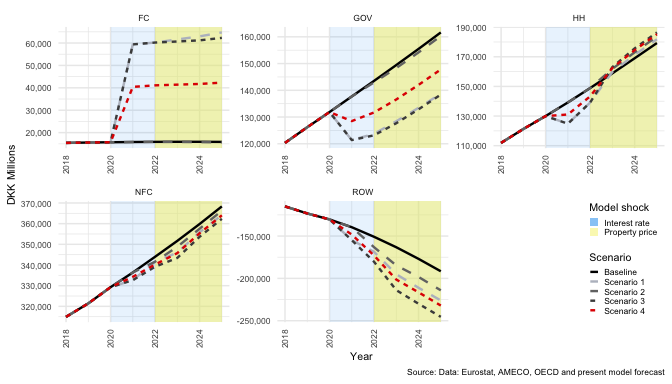
\includegraphics[width=0.95\linewidth]{figures/fl-fi-sfc-Savings-extra-1} \caption{Savings}\label{fig:fl-fi-sfc-Savings-extra}
\end{figure}

\begin{figure}[H]
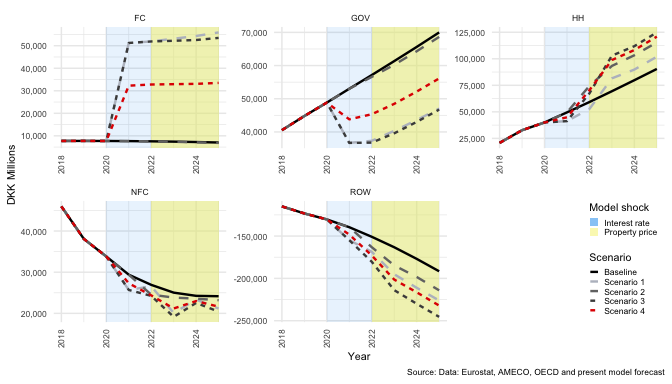
\includegraphics[width=0.95\linewidth]{figures/fl-fi-sfc-Yd-extra-1} \caption{Net Lending}\label{fig:fl-fi-sfc-Yd-extra}
\end{figure}

\begin{figure}[H]
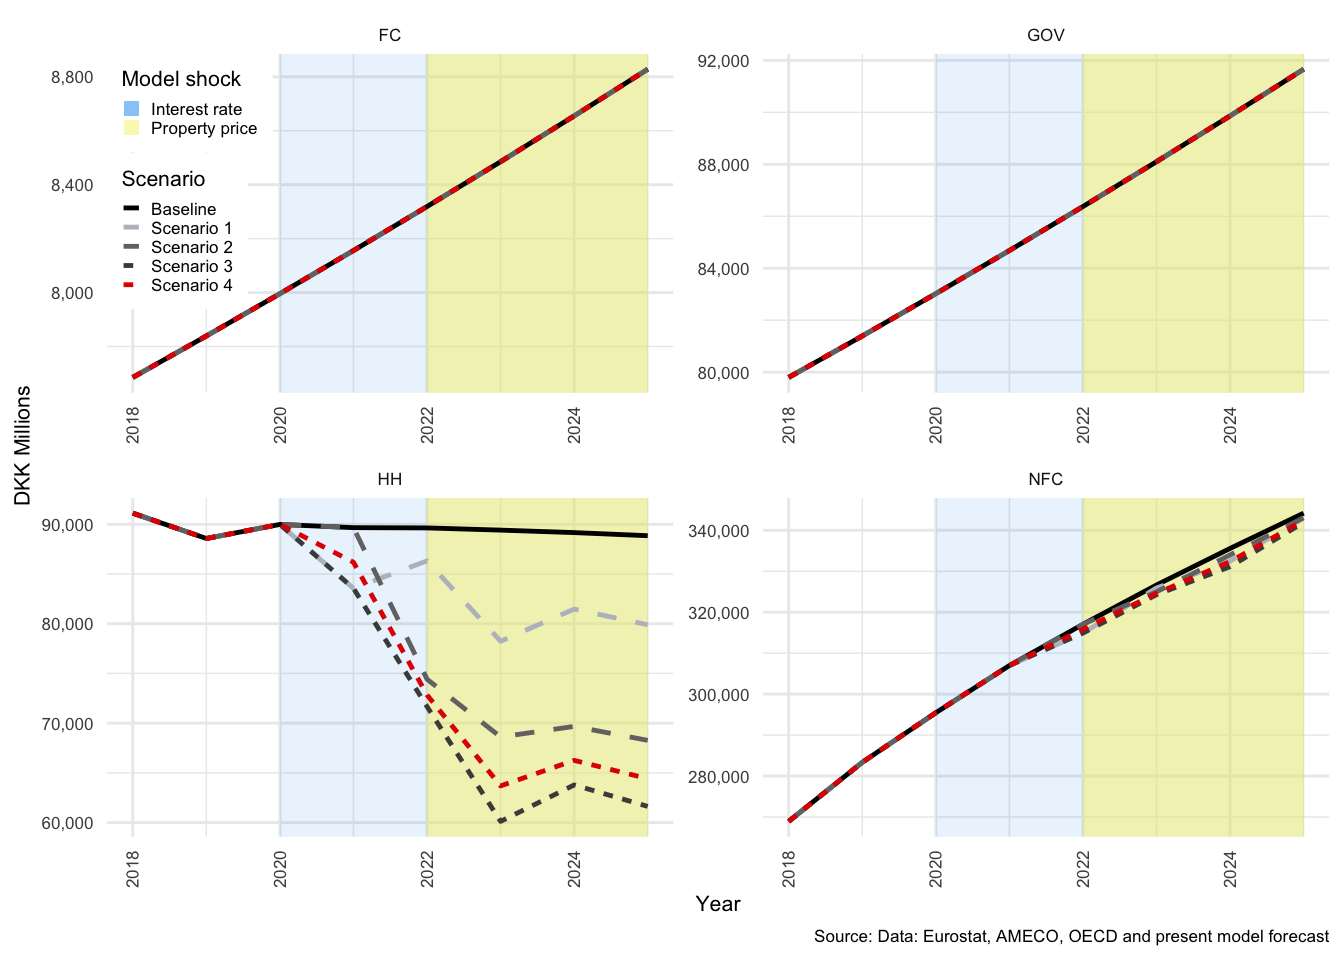
\includegraphics[width=0.95\linewidth]{figures/fl-fi-sfc-INV-extra-1} \caption{Investment}\label{fig:fl-fi-sfc-INV-extra}
\end{figure}

\hypertarget{residual-sector-flows}{%
\subsubsection{Residual sector flows}\label{residual-sector-flows}}

\begin{figure}
\centering
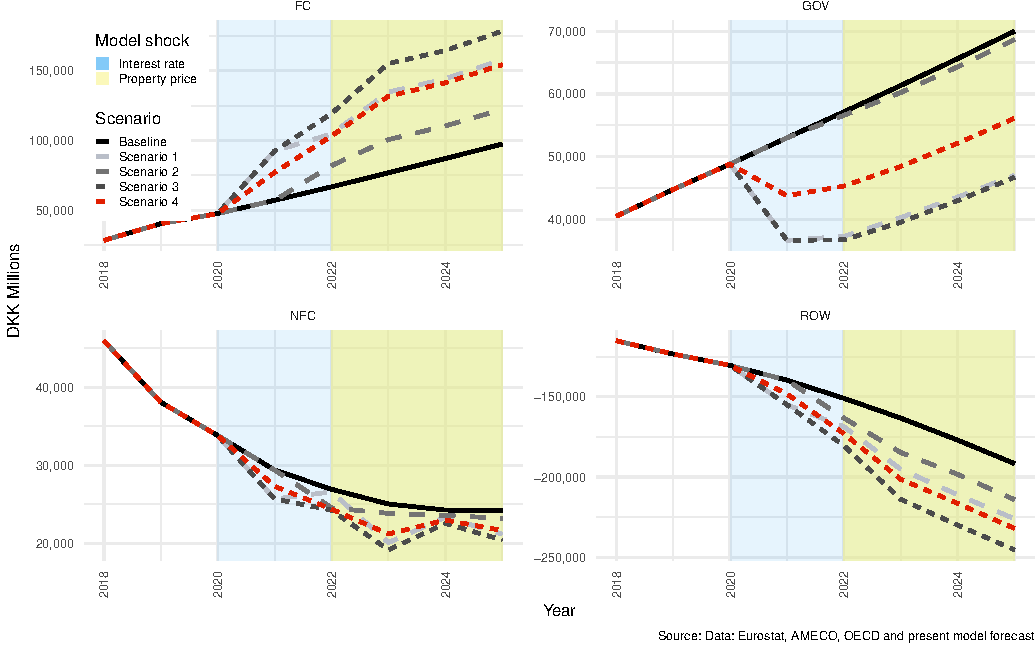
\includegraphics{figures/fl-fi-sfc-NIB-extra-1.pdf}
\caption{\label{fig:fl-fi-sfc-NIB-extra}Net interest bearing asset transactions}
\end{figure}

\begin{figure}[H]
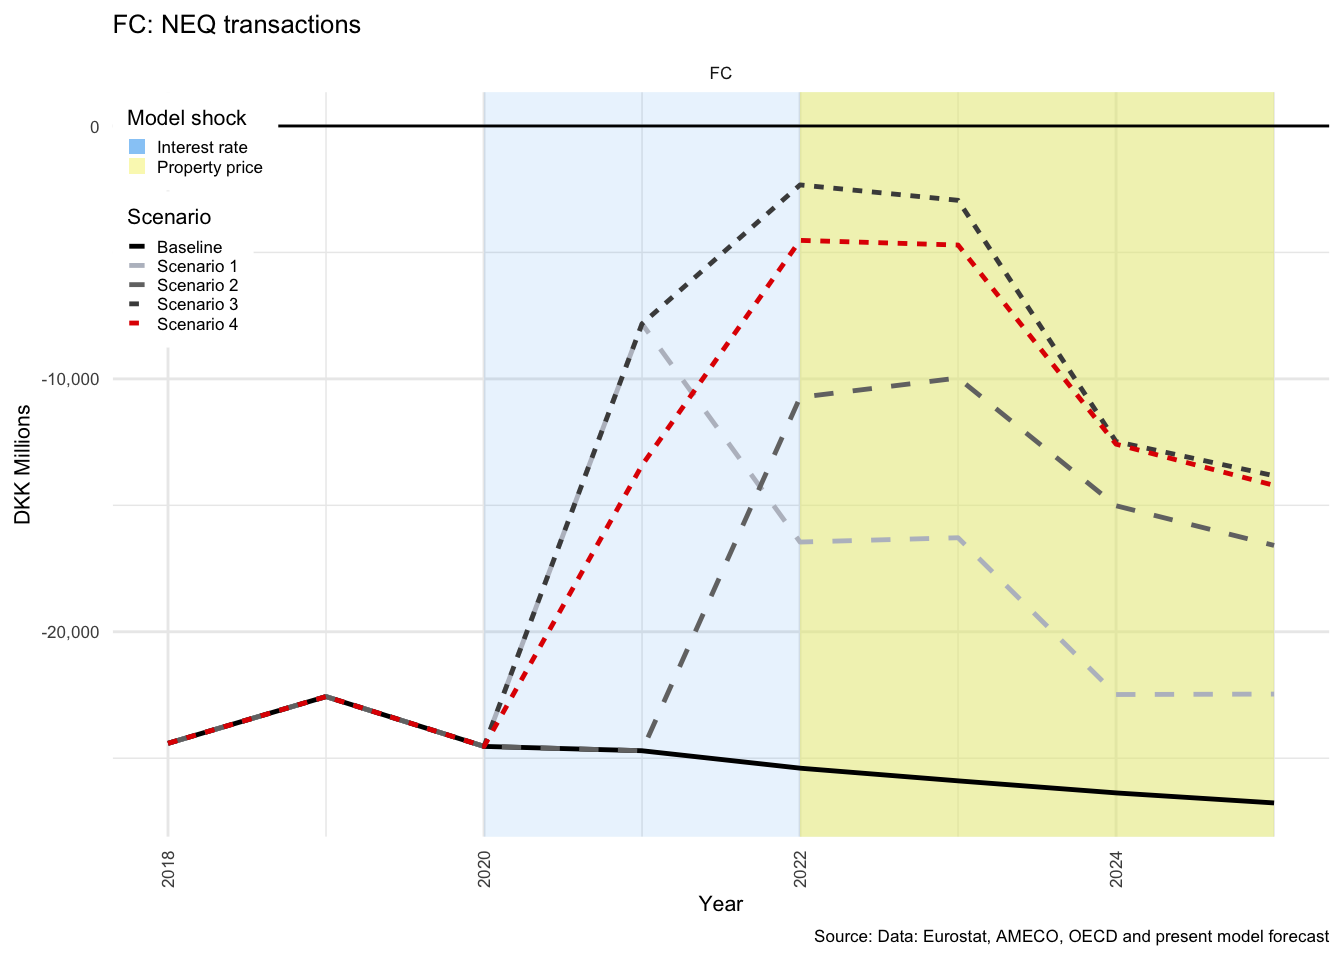
\includegraphics[width=0.5\linewidth]{figures/fl-fi-sfc-passive-FC-HH-1} \includegraphics[width=0.5\linewidth]{figures/fl-fi-sfc-passive-FC-HH-2} \caption{Residual flows for FC and HH}\label{fig:fl-fi-sfc-passive-FC-HH}
\end{figure}

\hypertarget{nw-nominal-prices-all-sectors}{%
\subsubsection{NW: Nominal prices: All sectors}\label{nw-nominal-prices-all-sectors}}

\begin{figure}
\centering
\includegraphics{figures/fl-fi-sfc-plot-fnw-1.pdf}
\caption{\label{fig:fl-fi-sfc-plot-fnw}NW: Nominal prices: All sectors}
\end{figure}

\hypertarget{capital-stock-nominal-prices-hh-nfc}{%
\subsubsection{Capital Stock: Nominal prices: HH, NFC}\label{capital-stock-nominal-prices-hh-nfc}}

\begin{figure}[H]
\includegraphics[width=0.95\linewidth]{figures/fl-fi-sfc-plot-k-1} \caption{Capital Stock: Nominal prices: HH, NFC}\label{fig:fl-fi-sfc-plot-k}
\end{figure}

\hypertarget{financial-transactions-nominal-prices-hh}{%
\subsubsection{Financial transactions: Nominal prices: HH}\label{financial-transactions-nominal-prices-hh}}

\begin{figure}
\centering
\includegraphics{figures/fl-fi-sfc-plot-fin-tr-HH-1.pdf}
\caption{\label{fig:fl-fi-sfc-plot-fin-tr-HH}Financial transactions: Nominal prices: HH}
\end{figure}

\hypertarget{financial-transactions-nominal-prices-nfc}{%
\subsubsection{Financial transactions: Nominal prices: NFC}\label{financial-transactions-nominal-prices-nfc}}

\begin{figure}
\centering
\includegraphics{figures/fl-fi-sfc-plot-fin-tr-NFC-1.pdf}
\caption{\label{fig:fl-fi-sfc-plot-fin-tr-NFC}Financial transactions: Nominal prices: NFC}
\end{figure}

\hypertarget{financial-transactions-nominal-prices-fc}{%
\subsubsection{Financial transactions: Nominal prices: FC}\label{financial-transactions-nominal-prices-fc}}

\begin{figure}
\centering
\includegraphics{figures/fl-fi-sfc-plot-fin-tr-FC-1.pdf}
\caption{\label{fig:fl-fi-sfc-plot-fin-tr-FC}Financial transactions: Nominal prices: FC}
\end{figure}

\hypertarget{financial-transactions-nominal-prices-gov}{%
\subsubsection{Financial transactions: Nominal prices: GOV}\label{financial-transactions-nominal-prices-gov}}

\begin{figure}
\centering
\includegraphics{figures/fl-fi-sfc-plot-fin-tr-GOV-1.pdf}
\caption{\label{fig:fl-fi-sfc-plot-fin-tr-GOV}Financial transactions: Nominal prices: GOV}
\end{figure}

\hypertarget{financial-transactions-nominal-prices-row}{%
\subsubsection{Financial transactions: Nominal prices: ROW}\label{financial-transactions-nominal-prices-row}}

\begin{figure}
\centering
\includegraphics{figures/fl-fi-sfc-plot-fin-tr-ROW-1.pdf}
\caption{\label{fig:fl-fi-sfc-plot-fin-tr-ROW}Financial transactions: Nominal prices: ROW}
\end{figure}

\hypertarget{iba-and-ibl-stock-fc}{%
\subsubsection{IBA and IBL: Stock: FC}\label{iba-and-ibl-stock-fc}}

\begin{figure}[H]
\includegraphics[width=0.95\linewidth]{figures/fl-fi-sfc-plot-a-l-f-1} \caption{IBA and IBL: Stock: FC}\label{fig:fl-fi-sfc-plot-a-l-f}
\end{figure}

\hypertarget{ibl-fixed-and-flexible-stocks-hh}{%
\subsubsection{IBL: Fixed and Flexible: Stocks: HH}\label{ibl-fixed-and-flexible-stocks-hh}}

\begin{figure}[H]
\includegraphics[width=0.95\linewidth]{figures/fl-fi-sfc-plot-ibl-h-1} \caption{IBL: Fixed and Flexible: Stocks: HH}\label{fig:fl-fi-sfc-plot-ibl-h}
\end{figure}

\hypertarget{sec:list-of-variables-shocks}{%
\subsection{Lists of variables from scenarios}\label{sec:list-of-variables-shocks}}

\textbackslash begin\{table\}

\textbackslash caption\{(\#tab:variable-names-table\_shocks)List of variables in scenario tables\}
\centering
\fontsize{10}{12}\selectfont

\begin{tabular}[t]{l|l|l}
\hline
Variable & Type & Description\\
\hline
ALPHA & Ratio & Ratio of fixed interest mortgage debt\\
\hline
B2 & Flow & Gross operating surplus\\
\hline
BETA,DATA & Parameter & Parameter\\
\hline
BOP & Flow & Balance of payments\\
\hline
C & Flow & Consumption\\
\hline
CAB & Flow & Current account balance\\
\hline
CGK & Flow & Capital gains\\
\hline
CGS & Flow & Capital gains\\
\hline
CHECK,B2 & Check & Consistency check: Gross operating surplus\\
\hline
CHECK,CTR & Check & Consistency check: Capital transactions\\
\hline
CHECK,EQ & Flow & Consistency check: Equity Transactions\\
\hline
CHECK,ERROR1 & Check & Consistency check: Error 1\\
\hline
CHECK,ERROR2 & Check & Consistency check: Error 2\\
\hline
CHECK,ERROR3 & Check & Consistency check: Error 3\\
\hline
CHECK,IB & Flow & Consistency check: Interest bearing transactions\\
\hline
CHECK,IB,TFLOW & Check & Consistency check: Interest bearing: Flows\\
\hline
CHECK,INVEST & Check & Consistency check: Investment\\
\hline
CHECK,NEQ & Flow & Consistency check: Net equity\\
\hline
CHECK,NIB & Check & Consistency check: Net interest bearing\\
\hline
CHECK,NIB & Flow & Consistency check: Net interest bearing\\
\hline
CHECK,NIB,TFLOW & Check & Consistency check: Net interest bearing: Flows\\
\hline
CHECK,NP & Check & Consistency check: Net purchases of non-financial assets (NP)\\
\hline
CHECK,NPEN & Flow & Consistency check: Net pensions: Revaluations\\
\hline
CHECK,PEN & Flow & Consistency check: Pensions: Transactions\\
\hline
CHECK,STRA & Check & Consistency check: Social transfers\\
\hline
CHECK,TAX & Check & Consistency check: Tax\\
\hline
CHECK,WAGE & Check & Consistency check: Wages\\
\hline
CPEN & Flow & Financial Liabilities: Change in pension entitlements\\
\hline
CTR & Flow & Capital transfers\\
\hline
CU & Ratio & Capacity Utilisation (Real GNI  /  real capital stock)\\
\hline
D,1998 & Dummy & Dummy variable: 1998\\
\hline
D,200 & Dummy & Dummy variable: 2000\\
\hline
D,2004 & Dummy & Dummy variable: 2004\\
\hline
D,2006 & Dummy & Dummy variable: 2006\\
\hline
D,2007 & Dummy & Dummy variable: 2007\\
\hline
D,2008 & Dummy & Dummy variable: 2008\\
\hline
D,2009 & Dummy & Dummy variable: 2009\\
\hline
D,2010 & Dummy & Dummy variable: 2010\\
\hline
D,2011 & Dummy & Dummy variable: 2011\\
\hline
D,2014 & Dummy & Dummy variable: High taxes: 2014\\
\hline
D,2015 & Dummy & Dummy variable: 2015\\
\hline
D,2016 & Dummy & Dummy variable: 2016\\
\hline
D21 & Flow & Taxes on products\\
\hline
D29 & Flow & Other taxes on production\\
\hline
D31 & Flow & Subsidies D31\\
\hline
D39 & Flow & Subsidies D39\\
\hline
D41,P & Flow & Interest: Paid\\
\hline
D41,R & Flow & Interest: Received\\
\hline
D41B & Flow & Interest: Received\\
\hline
D42,P & Flow & Distributed income of corporations: Paid\\
\hline
D42,R & Flow & Distributed income of corporations: Received\\
\hline
D44,P & Flow & Other investment income: Paid\\
\hline
D44,R & Flow & Other investment income: Received\\
\hline
DELTA & Ratio & Equity to assets ratio\\
\hline
DEP & Flow & Depreciation of fixed capital\\
\hline
EQA & Flow & Financial Assets: Equity assets\\
\hline
EQA & Stock & Financial Assets: Equity assets\\
\hline
EQA,R & Ratio & Equity ratio\\
\hline
EQL & Flow & Financial Liabilities: Equity liabilities\\
\hline
EQL & Stock & Financial Liabilities: Equity liabilities\\
\hline
ERROR,CHECK1 & Check & Error check\\
\hline
ERROR,CHECK2 & Check & Error check\\
\hline
ERROR,CHECK3 & Check & Error check\\
\hline
FA & Flow & Financial Assets\\
\hline
FA & Stock & Financial Assets\\
\hline
FAB & Flow & Financial account balance\\
\hline
FEE59 & Ratio & Danish exports to trading partners: Weighted average total exports (imports by foreign trading partners)\\
\hline
FL & Flow & Financial liabilities\\
\hline
FL & Stock & Financial liabilities\\
\hline
FNL & Flow & Financial Net Lending (Balance)\\
\hline
FNW & Stock & Financial net wealth\\
\hline
G & Flow & Government expenditure\\
\hline
GDP & Flow & Gross domestic product\\
\hline
HFHF & Check & Test variable: Not used\\
\hline
I & Flow & Gross fixed capital formation\\
\hline
IBA & Flow & Financial Assets: Interest bearing assets\\
\hline
IBA & Stock & Financial Assets: Interest bearing assets\\
\hline
IBL & Flow & Financial Liabilities: Interest bearing liabilities\\
\hline
IBL & Stock & Financial Liabilities: Interest bearing liabilities\\
\hline
IBL,RV1 & Flow & Financial Liabilities: Interest bearing liabilities\\
\hline
INFL & Rate & Inflation rate: Price inflation\\
\hline
INFL,M & Rate & Inflation rate: Price inflation: Foreign\\
\hline
INV & Flow & Gross fixed capital formation\\
\hline
K & Stock & Stock of Capital\\
\hline
K,CG & Flow & Capital Gains\\
\hline
KCG & Flow & Capital Gains\\
\hline
KCG,SUM & Flow & Capital Gains - Cummulative sum\\
\hline
LEV & Ratio & Leverage ratio: NFC: Funding liabilities to GDP\\
\hline
LEV1 & Ratio & Leverage ratio: NFC: Funding liabilities\\
\hline
LF & Stock & Labour force: Total number of employable persons\\
\hline
M & Flow & Imports\\
\hline
N & Stock & Labour force: Denmark for workers in production\\
\hline
NEQ & Flow & Net financial stock: Equity\\
\hline
NEQ & Stock & Net financial stock: Equity\\
\hline
NF & Stock & Labour force: Employed persons: Danish waged\\
\hline
NIB & Flow & Net financial stock: Interest bearing\\
\hline
NIB & Stock & Net financial stock: Interest bearing\\
\hline
NL & Flow & Sector Balance\\
\hline
NL,CHECK & Check & Consistency check: Net lending\\
\hline
NP & Flow & Net purchases of non-financial assets (NP)\\
\hline
NPEN & Flow & Net financial stock: Pension\\
\hline
NPEN & Stock & Net financial stock: Pension\\
\hline
NPIR & Flow & Net property income received: Total\\
\hline
NPIR,NEQ & Flow & Net property income received: NEQ\\
\hline
NPIR,NIB & Flow & Net property income received: NIB\\
\hline
NPIR,NPEN & Flow & Net property income received: NPEN\\
\hline
NU & Stock & Labour force: Employed persons: Danish nationals: Employed abroad\\
\hline
NW & Stock & Net Wealth\\
\hline
NX & Flow & Net Exports\\
\hline
OTR & Flow & Other current transfers\\
\hline
P,CGK & Deflation index & Price index: Capital gains\\
\hline
P,NEQ & Deflation index & Price index: Net Equity\\
\hline
P,NIB & Deflation index & Price index: Net interest bearing assets\\
\hline
P,PEN & Deflation index & Price index: Pensions\\
\hline
PC & Deflation index & Price deflator: Consumption\\
\hline
PE & Deflation index & Price deflator: Unknown\\
\hline
PENA & Flow & Financial Assets: Pension assets\\
\hline
PENA & Stock & Financial Assets: Pension assets\\
\hline
PENL & Flow & Financial Liabilities: Pension liabilities\\
\hline
PENL & Stock & Financial Liabilities: Pension liabilities\\
\hline
PG & Deflation index & Price deflator: Government consumption\\
\hline
PH & Deflation index & Price deflator: Houses\\
\hline
PH01 & Deflation index & Price deflator: Houses (Alternative)\\
\hline
PHI1 & Flow & Social contributions to income\\
\hline
PHI2 & Flow & Pension transactions to social contributions\\
\hline
PI & Deflation index & Price deflator: Investment (weighted average of deflators for housing(pk) and all other investment (pk)) . Proportion of dwellings in total investment is approx 0.22, and pi closely resembles the deflator for total investment reported by ameco.\\
\hline
PIP & Flow & Property income paid\\
\hline
PIP,IBL & Flow & Property income paid: IBL\\
\hline
PIP,PENL & Flow & Property income paid: PENL\\
\hline
PIR & Flow & Property income received\\
\hline
PIR,EQA & Flow & Property income received: EQA\\
\hline
PIR,IBA & Flow & Property income received: IBA\\
\hline
PIR,PENA & Flow & Property income received: PENA\\
\hline
PK & Deflation index & Price deflator: Investment (excluding dwellings)\\
\hline
PM & Deflation index & Price deflator: Imports\\
\hline
PNFC & Deflation index & Price deflator: NFC K\\
\hline
POP & Stock & Population\\
\hline
PP & Check & Unknown\\
\hline
PRIVATE & Flow & Gross income\\
\hline
PROD & Stock & Labour Force: Labour productivity\\
\hline
PROFIT & Ratio & Profit share (Residual of wage share)\\
\hline
PX & Deflation index & Price deflator: Exports\\
\hline
PY & Deflation index & Price deflator: GDP\\
\hline
R,EQ & Rate & Rate of return: Equities\\
\hline
R,ERROR1 & Check & Property income error\\
\hline
R,ERROR2 & Check & Property income error\\
\hline
R,ERROR3 & Check & Property income error\\
\hline
R,IBA & Rate & Rate of interest: Interest bearing assets\\
\hline
R,IBL & Rate & Rate of interest: Interest bearing liabilities\\
\hline
R,IBL,SENS & Rate & Rate of interest: Interest bearing liabilities: Weighted mortgage interest rate\\
\hline
R,N & Rate & Rate of return: Mean\\
\hline
R,NET,ERROR1 & Check & Property income error\\
\hline
R,NET,ERROR101 & Check & Property income error\\
\hline
R,NET,ERROR2 & Check & Property income error\\
\hline
R,NET,ERROR201 & Check & Property income error\\
\hline
R,NET,ERROR3 & Check & Property income error\\
\hline
R,NET,ERROR301 & Check & Property income error\\
\hline
R,PEN & Rate & Rate of return: Pensions\\
\hline
R,R,IBL & Rate & Rate of interest: Interest bearing liabilities\\
\hline
RHO & Ratio & Equity ratio\\
\hline
RR & Rate & Rate of return\\
\hline
S & Flow & Savings\\
\hline
SBE & Flow & Social benefit transfers\\
\hline
SCO & Flow & Social benefit contributions\\
\hline
STRA & Flow & Social transfers\\
\hline
T & Flow & Taxes on products\\
\hline
TAX & Flow & Tax\\
\hline
TEST & Check & Test variable: Stock of Capital (Change in)\\
\hline
TOBIN,Q & Index & Index: House price index: Tobin's Q = Ratio between the house price index and the construction cost of housing index\\
\hline
TOP & Ratio & Ratio of foreign to domestic trade\\
\hline
UL,COST & Rate & Labour force: Unit labour cost\\
\hline
ULC & Rate & Labour force: Unit labour cost: Price index: Index for the price deflator with reference to 2010 (all other price deflator indices are referenced to 2010)\\
\hline
UN & Stock & Labour force: Unemployed persons\\
\hline
UR & Ratio & Labour force: Unemployment rate\\
\hline
W & Flow & Wages\\
\hline
WAGE & Rate & Labour force: Wage rate\\
\hline
WI & Rate & Inflation rate: Wage inflation\\
\hline
WS & Ratio & Wage share\\
\hline
X & Flow & Exports\\
\hline
XR & Rate & Exchange rate\\
\hline
Y & Flow & Total income\\
\hline
Y,D & Flow & Disposable Income\\
\hline
YEAR &  & \\
\hline
ZZ & Index & Index: House price index\\
\hline
ZZ,I & Index & Index: House price: Imported from DST\\
\hline
ZZ,INDEX & Index & Index: House price: Mark-up pricing on construction costs\\
\hline
ZZ1 & Index & Index: House price: Imported from DST\\
\hline
\end{tabular}

\textbackslash end\{table\}

\hypertarget{sec:fi-fl-sfc-full-model}{%
\section{Complete set of model equations}\label{sec:fi-fl-sfc-full-model}}

\hypertarget{sec:fi-fl-sfc-model-eq-nf}{%
\subsection{Non-Financial Corporate Sector}\label{sec:fi-fl-sfc-model-eq-nf}}

The following appendix is adapted from \citet{byrialsenraza2019empirical}, except otherwise indicated.
It is included here for completeness in the explanation of the structure of
the model. As in their model, the non-financial corporate sector (NFC) is responsible for all production,
where total nominal production is represented as:

\begin{equation}
Y_t = C_t + I_t + G_t + X_t - M_t
\label{eq:ynominal}
\end{equation}

This can be rewritten in terms of sales, or rather, from an income perspective:

\begin{equation}
S_t = C_t + I_t + G_t + X_t
\label{eq:nfcsales}
\end{equation}

The production equation from Equation (\ref{eq:ynominal}) can be deflated to real prices;

\begin{equation}
y_t = c_t + i_t + g_t + x_t - m_t
\end{equation}

Where the GDP deflator can be represented as:

\begin{equation}
P^y_t = \frac{Y_t}{y_t}
\end{equation}

Outflows for NFC include taxes paid to GOV, wages (\(WB\)) paid to domestic and foreign households, and profits (\(B2\)\footnote{Profits here refer to the gross operating surplus for the sector, ESA non financial transactions item \(B2\).}).

\begin{equation}
WB^N_t = W_t(N^N_t)
\end{equation}

The nominal wage bill is calculated as the wage rate (\(W_t\)) times the
level of employment (\(NN_t\)), where \(NN_t\) includes all domestic employment
of citizens plus the net employment of foreigners in Denmark and Danish citizens abroad.

Taxes paid by NFC are predominantly production based and are therefore
calculated as a proportion of total production in each period (\(Y_t\)).

\begin{equation}
T^N_t = \beta _3(Y_t)
\end{equation}

It is assumed that firms target a fairly stable level of mark-up on production,
and thus \(B2\) is calculated as an estimated proportion of \(Y_t\).

\begin{equation}
B2_t = \beta Y_t
\end{equation}

The stock of NFC fixed capital, (\(K^N_t\)), is diverse, and is calculated via the
standard accounting method, allowing for capital accumulation via investment (\(I^N_t\)),
depreciation (\(D^N_t\)) and capital gains (\(K^N_{CG_t}\)).

\begin{equation}
K^N_t = K^N_{t-1} + I^N_t - D^N_t + K^N_{CG_t}
\end{equation}

Depreciation of capital is assumed to apply to stock held at the end of the previous
period.

\begin{equation}
D^N_t = \delta (K^N_{t-1})
\end{equation}

The capital deflator (\(P^i_t\)) can then be used to calculate the real
value of the stock of capital in each period.

\begin{equation}
k^N_t = \frac{K^N_t}{P^i_t}
\label{eq:realcap}
\end{equation}

Investment is estimated in real terms as a function of capacity utilisation.

\begin{equation}
ln(i^N_t) = \beta _i + ln\beta _i. \Bigg( \frac{y_{t-i}}{k^N_{t-i}}\Bigg)
\end{equation}

It can then be inflated to current prices using the same capital price deflator as in Equation (\ref{eq:realcap}), \(P^i_t\).

\begin{equation}
I^N_t = i^N_t(P^i_t)
\end{equation}

NFC savings (\(S^N_t\)), not to be confused with sales (\(S_t\)) in Equation (\ref{eq:nfcsales}),
can be calculated as the net sum primary and secondary income and expenditures.

\begin{equation}
\begin{split}
S^N_t = & Y_t - WB^N_t + (B2^N_{t} - B2_{t}) + r^N_{t-1}(NIB^N_{t-1})\\
        & + \chi _t (NEQ^N_{t-1}) - T^N_t + STR^N_t + \epsilon ^N
\end{split}
\end{equation}

Net lending (\(NL^N\)) takes into account the additional sources of change
originating from fixed asset adjustments. In particular, \(NP\) is the net
sale and acquisition of non-financial assets, savings and investment reflect
\emph{ex post} portfolio decisions, and finally \(KTR^N\) represents any additional
capital transfers. \footnote{This structure follows for each of the sectors, with the exception of the rest of the world sector (ROW), where ownership of fixed assets is not included, and therefore, by definition, neither is investment. \(NP\) is determined exogenously, and is for the most part of negligible size.} NFC is also assumed to receive all
income from production in the economy, and thus the level of operating surplus must
be adjusted to take into account that of all other sectors, thus NFC retains
(\(B2^N_{t} - B2_{t}\)) gross operating surplus. The \(\epsilon ^N\) refers to adjustments made to ensure stock and flow consistency in the level of property income received or paid during the periods where data was available\footnote{This convention is used for all sectors. The returns on financial assets are estimated with varying degrees of accuracy for each of the sectors. In order to ensure that the model is consistent in all periods, any difference between the estimated returns and actual returns (on a net basis for each asset class) are added to the adjustment term. These errors in estimation are minimised in the estimation specification for each asset class individually.}.

\begin{equation}
NL^N_t = S^N_t - I^N_t- NP^N_t + KTR^N
\end{equation}

The calculation of stocks for each of the classes held by NFC are in equations (\ref{eq:nfc-neq})
and (\ref{eq:nfc-nib}).

Net equities:

\begin{equation}
NEQ^N_t = NEQ^N_{t-1} + NEQTR^N_t + NEQ^N_{CG_t}
\label{eq:nfc-neq}
\end{equation}

Net interest bearing stocks:

\begin{equation}
NIB^N_t = NIB^N_{t-1} + NIBTR^N_t + NIB^N_{CG_t}
\label{eq:nfc-nib}
\end{equation}

Net interest bearing assets, like several others in this model, are determined
by a combination of previous stocks (\(NIB^N_{t-1}\)), transactions (\(NIBTR^N_t\))
and capital gains (\(NIB^N_{CG_t}\)). The transactions component of interest
bearing assets for NFC is determined passively. It is calculated as the remainder
of Savings, after capital transfers, and after portfolio allocation towards
equities. Transactions in equities (\(NEQTR^N\)) are thus the active component of the composition
of the NFC balance sheet portfolio.

\begin{equation}
NIBTR^N_t = NL^N_t - NEQTR^N_t
\end{equation}

Since NFC only holds these two financial assets in the model, the sum constitutes the
financial net wealth (\(FNW^N\)) of NFC.

\begin{equation}
FNW^N_t = NIB^N_t + NEQ^N_t
\end{equation}

This is different to the total net wealth (\(NW^N\)), which also includes the fixed capital
(\(K^N\)) owned by NFC.

\begin{equation}
NW^N_t = FNW^N_t + K^N
\end{equation}

\hypertarget{sec:fi-fl-sfc-model-eq-hh}{%
\subsection{Household Sector}\label{sec:fi-fl-sfc-model-eq-hh}}

The household sector (HH) is the primary focus of this model, in particular the interest bearing
liabilities of the household sector, and the drivers thereof. It is therefore the sector with
most endogenous components. Equation (\ref{eq:Yht}) describes the incomes and expenditures
of HH. The primary sources of which are wages (\(WB^H\)), profits (\(B2\)), property income
(or returns on financial capital, which stems from interest bearing assets, \(IBA^H\),
pensions, \(PENA^H\), and equities, \(EQA^H\)), and social transfers(\(STR^H\)).

\begin{equation}
\begin{split}
Y^H_t = & WB^H_t + B2^H_{t} + r^H_{A_{t-1}}(IBA^H_{t-1})\\
        & - r^H_{L(FI)_{t-1}}(IBL(FI)^H_{t-1})\\
        & - r^H_{L(FL)_{t-1}}(IBL(FL)^H_{t-1})\\
        & + \chi _t(EQA^H_{t-1}) + \psi _t(PENA^H_{t-1}) + STR^H_t + \epsilon ^H
\label{eq:Yht}
\end{split}
\end{equation}

Interest rates are represented by \(r^H\), and the ``A'' (``L'') subscript referring to the assets (liabilities), and (\(\chi _t\)) and (\(\psi _t\)) are the rates of return on equities and pensions. As part of the key change in this model, the level of interest paid on \(IBL\) in this model is split between fixed and flexible rate mortgages into \(r^H_{L(FI)_{t-1}}(IBL(FI)^H_{t-1})\) and \(r^H_{L(FL)_{t-1}}(IBL(FL)^H_{t-1})\). A similar split is present in the financial corporate sector (FC) below.

Social transfers received by the households in the above equations is the sum of social contribution (\(SCON^H\)) paid by the households, social benefits (\(SBEN^H_t\)), and other transfers (\(OTR^H\)) received by the households:
Social transfers:

\begin{equation}
STR^H_t = SBEN^H_t + OTR^H_t - SCON^H
\end{equation}

Total taxes paid by households are a relatively constant proportion of income over time,
and are deducted from total income to give disposable income:

\begin{equation}
YD^H_t = Y^H_t - T^H_t
\end{equation}

The total value of tax payment by households is assumed to be a constant portion (\(\beta _i\))
of household primary and secondary income.

\begin{equation}
T^H_t = \beta _i (Y^H_t)
\end{equation}

The level of social contributions are a proportion of disposable income, adjusted over time.

\begin{equation}
SCON^H_t = \beta _7(YD^H_{t-i})
\end{equation}

The largest components of \(SBEN^H\) are pension and medical payments. \citet{byrialsenraza2019empirical},
modelled changes in benefits against changes in the the wage rate and
the level of unemployment. Although not directly related to the main components of
benefits, they appear to be good proxies for changes in pension distributions, which
in some cases may be based on emoluments.

\begin{equation}
ln(SBEN^H_t) = \beta _i + \beta _i ln(U^N_t) + \beta _i ln(W^H_{t-i})
\label{eq:socialbenefits}
\end{equation}

Since 2007, approximately 35\% - 37\% of all social benefits
were for old age payments. A further 20\% - 22.3\% are attributed to medical benefits, an almost
constant 14.4\% to disability and 10\% - 13.2\% to family and child benefits. Unemployment (app. 5\%),
social exclusion (app. 5\%), housing (app. 2\%) and survivorship (app. 1\%) benefits making up the balance.

\begin{figure}
\centering
\includegraphics{figures/sben-all-dk-1.pdf}
\caption{\label{fig:sben-all-dk}Social benefits by category}
\end{figure}

The old age category, as can be seen from Figure \ref{fig:old-age-public-spend},
is then dominated by tax funded pension payouts (app. 50\% in 2017),
old age accommodation and care (app. 15\%) and civil (app. 11\%) and other pension
schemes (app. 12\%), with the declining anticipated pension allocations (app. 5.2\% in 2017)
and growing labour market supplementary pension benefits (ATP\footnote{ATP is an anagram for \emph{Arbejdsmarkedets Tillægspension}, which translates directly to
  \emph{labour market supplementary pension}.}) (app. 5.8\%) making up the
balance. The full amount therefore could be considered as pension income, but since these
pension benefits are funded predominantly by tax, rather than from assets, they are best
kept separate from the capital income on pension assets described in Equation (\ref{eq:Yht})
above. This is perhaps with the exception of labour market supplementary pension benefits, which are
payouts from a pooled investment portfolio.

\begin{figure}
\centering
\includegraphics{figures/old-age-public-spend-1.pdf}
\caption{\label{fig:old-age-public-spend}Old age social benefits}
\end{figure}

This is not merely a question of semantics, as the old age component is also an element
of wage negotiations for the working population. A large part of social contributions (\(SCON^H\))
are also contributions towards the labour market pension fund.\footnote{The Danish pension system is beyond the scope of this discussion,
  but a brief summary may be useful here. As described by \citet[pp.~2]{andersen2016dps}, the
  system is relatively complex three pillar system, with the most recent comprehensive
  reform taking place in 1964. The three pillars are:
  1.) A state pension (with several minor schemes),
  2.) Semi-mandatory occupational pensions (or labour market pensions), and
  3.) Personal pension savings.
  The state pension and other peripheral benefits (such as old age accommodation support,
  heating support etc) is tax funded and essentially a flat rate benefit for all citizens,
  while the second and third pillars are savings based, and thus have been slower to mature.
  There have been a range of relatively minor adjustments to the state pension system over
  the past few decades, some of which are adjustments according to what other benefits or
  income the person has (partially means tested). The conditions of the occupational pension
  system, much like much of the labour market working conditions agreements, are determined
  via collective agreement. While there are no legislated wage or pension requirements - for
  example there is no minimum wage in Denmark - the coverage of collective bargaining
  agreements is almost universal. \citep{andersen2016dps}}
\(SBEN^H\) is, perhaps understandably, the second largest component of HH disposable income in Denmark.
As can be seen in Figure \ref{fig:sben-all-dk}, this can quickly be understood to be driven
primarily by healthcare and pensions, but in a more general sense, by components of the strong
Danish welfare system. Labour market pension payouts are expected to fall (rise), as are unemployment
benefit payouts, as economic conditions improve (deteriorate). Unemployment, as an indicator of economic
distress, appears to be a good proxy for expected changes in benefit payouts relative to total HH
disposable income. Equation (\ref{eq:socialbenefits}) captures this effect, together with the
effect of changes in the wage rate. The latter because unemployment benefits and several pension
benefits are adjusted according to changes in industry wage rates, as noted by \citet{byrialsenraza2018}
and \citeyearpar{byrialsenraza2019empirical}.

Real disposable income, as will be the case for several other variables in this model, can be
calculated by dividing household disposable income by a consumption price index (\(P^c\)).

\begin{equation}
yd^H_t = \frac{YD^H_t}{P^c_t}
\end{equation}

Consumption, like NFC investment, is estimated in real terms in a standard Keynesian form, and
log-linearised for stationarity. Consumption is taken to be determined by a combination of
real disposable income and household wealth of the preceding period. Although not explicitly
modelled, current consumption thus is assumed to be based purely on expectations developed
in the previous period.

\begin{equation}
ln(c_t) = \beta _0 + \beta _iln(yd^H_{t-i}) + \beta _iln(nw^H_{t-1})
\label{eq:hh_consumption}
\end{equation}

Nominal consumption can be calculated using the consumption price index to inflate the series.

\begin{equation}
C_t = c_t(P^c_t)
\end{equation}

\(P^c\), the consumption price index is endogenous to changes in the wage rate and
the import price index from the previous period. In some way reflecting a delayed adjustment
in (or, sticky) prices, and the importance of international prices for smaller open economies,
such as Denmark.

\begin{equation}
ln(P^c_t) = \beta _0 + \beta _iln(W_{t-i}) + \beta _iln(P^m_{t-i})
\end{equation}

The following equations are related to household interactions with capital an investment
markets.

In this model, households are only permitted to make productive investment in
housing, which, in this model, is considered only as a
primary market, following \citet{Zezza2008}, \citet{fontana2013securitization} and \citet{beckta2015modelling}.
The secondary market for houses is assumed to affect prices, but not the demand
for additional housing investment. Demand for housing investment is determined by
by a Tobin's-Q-like function, partially driven by changes in disposable income and
previous period housing investment, and partially driven by a relative shift in
sales price (\({P^H_{t-i}}\)) and construction cost (\({P^i_{t-i}}\)) indices.

Real investment in fixed assets (dwellings):

\begin{equation}
ln(i^H_t) = \beta _i + \beta _i ln(i^H_{t-i}) + \beta _i ln \Bigg( \frac{P^H_{t-i}}{P^i_{t-i}}\Bigg) + \beta _iln(yd^H_{t-i})
\label{eq:housing-hh}
\end{equation}

As noted by \citet[pp.~20]{byrialsenraza2019empirical}, ``The intuition behind the above equation is straight forward, i.e., an increase in the house prices motivates the households to invest more in the construction of new houses, while an increase in the construction costs would lower housing investment.''

A shift downwards in house prices would conversely reduce overall returns on houses relative to
construction costs, and thus result in a decline in the demand for housing investment.
This would result, all else equal, in an increase in savings and a consequent rise in the demand
for alternative outlets. Limited below to the purchase of financial assets\footnote{\citet{andre2016household}, in a recent OECD working paper argue that while there is an
  obvious connection between the availability of credit and house prices, the extent to which
  house prices are affected by changes in mortgage lending is affected by a wide range of
  factors, including sentiment, employment conditions, legislative changes, and a range of cyclical
  economic factors. \citet{kohlscheen2018residential} also note the co-movement of residential property
  prices and credit as a prominent feature of models of financial cycles, although their focus is
  on commonalities in financial, demographic and real economy factors. Their
  \citep[pp.~2]{kohlscheen2018residential} findings suggest that the primary drivers are
  ``real house prices, nominal interest rates, demographic factors, and the state of housing supply''.
  The present model captures all but demographic factors in the determination of residential (HH)
  investment. They also find strong asymmetries in the effects of interest rates between boom and
  bust cycles, and with rising interest rates rather than falling. This is supported by \citet{scanlon2008}'s
  findings that household mortgage lending is highly sensitive to short-term budget
  implications of interest and capital repayment costs.}.

The nominal level can be calculated by inflating the real investment in housing
series (\(i^H_t\)) by the investment price index (\(P^i_t\)):

\begin{equation}
I^H_t = i^H_t(P^i_t)
\end{equation}

The nominal stock of housing (\(K^H\)), as with other assets to come, follows the simple
process of previous stock, plus acquisition (in this case investment in new houses),
less depreciation (or disposal) plus capital gains.

\begin{equation}
K^H_t = K^H_{t-1} + I^H_t - D^H_t + K^H_{CG_t}
\end{equation}

Capital gains on houses, in turn, are calculated as:

\begin{equation}
KH_{CG} = \Delta P^H_t (K^H_{t-1})
\end{equation}

Which is simply the change in the price of houses applied to the level of stock at
the end of the preceding period.
The change in house prices leading into the current period is then by definition the same
ratio proportion of capital gains to previous housing capital.

\begin{equation}
\Delta P^H_t = \frac{KH_{CG}}{K^H_{t-1}}
\label{eq:changehouseprice}
\end{equation}

Nominal housing capital held by HH at the end of the current period
can be expressed as the price adjusted stock at the end of the previous
period, plus net investment and depreciation.

\begin{equation}
K^H_t = K^H_{t-1}(1 + \Delta P^H_t) + I^H_t- D^H_t
\end{equation}

The deflated real capital index can then be found by dividing the series by the
investment (housing) price index, as in Equation (\ref{eq:changehouseprice}) above.

\begin{equation}
k^H_t = \frac{K^H_t}{P^i_t}
\end{equation}

The level of savings is then calculated as a residual disposable income after
consumption and net pension adjustments - the ESA 2010 \citep{ESA2010} definition
of which is net of contributions, disbursements and returns of pension funds.

\begin{equation}
S^H_t = YD^H_t - C^H_t + CPEN^H_t
\end{equation}

Net lending can then be calculated savings plus additional consideration for the
net acquisition and disposal of fixed assets (\(NP\)) and capital transfers (\(KTR\))
less investment (assumed here to be solely in houses).

\begin{equation}
NL^H_t = S^H_t - I^H_t - NP^H_t + KTR^H_t
\end{equation}

HH must also fund real activities and allocate any excess funds in the financial markets.
As noted above, HH is the sector with most endogenous components in this model. It is
also the sector, together with the financial corporate sector (FC) that has the most complex financial accounts.
As noted by \citet{byrialsenraza2019empirical}, financial market changes in this model are
driven primarily by the demand for credit and assets. As they explained, transmission
is from flows to stocks. The behaviour is primarily modelled in transaction decisions,
and stocks are then calculated as the sum of these together with capital gains.

The net effect of annual changes in the financial position of HH is captured by
financial net lending. This is the sum of changes in financial assets less the
sum of changes in financial liabilities:

\begin{equation}
FNL^H_t = FATR^H_t - FLTR^H_t
\end{equation}

Household financial assets are held in interest bearing assets (\(IBA\)), equities\footnote{The equity component in the balance sheets of the other sectors in this model
  is limited to a net equity position. It is assumed here that HH do not issue equities.} (\(EQA\)) and
pensions (\(PENA\)). Transactions in each of these sum to make up the total
transactions in financial assets.

\begin{equation}
FATR^H_t = IBATR^H_t + EQATR^H_t + PENATR^H_t
\end{equation}

Transactions in equities are determined by a Tobin allocation matrix, thus enforcing a
budget constraint on HH, where the investment decision of the sector is determined at
least in part by relative rates of return. One exception is pension allocations, where a
fairly constant portion of HH income is allocated to pension investments, irrespective of
the rate of return. This leaves equities and interest bearing assets.

Demand for equities is negatively affected by increases in the returns available on interest
bearing assets in the previous period (\(\beta\) on \(r^H_{A_{t-1}}\)), positively related to
returns on equities (\(\chi\)), and positively related to increases in the extension of
credit (\(\beta\) on \(IBLTR^H\)).

\begin{equation}
EQATR^H_t = \beta _i + \beta _i(\chi _t) + \beta _i(r^H_{A_{t-1}}) + \beta _i(IBLTR^H_t )
\end{equation}

The link with \(IBL\) is associated with the investment incentive for more sophisticated
investors, where low interest rate debt can be used to arbitrage higher returns on
equities.

Pension transactions, in addition to the fixed proportion that is reflected
as a constant in the equation below, are positively affected by returns on pensions (\(\psi\))
and the wage bill (\(WB\)). Pensions transactions can thus be affected directly by the
wage rate, or the level of employment (and thus negatively by a rise in unemployment).

\begin{equation}
PENATR^H_t = \beta _i + \beta _i(\psi _t) + \beta _iWB^H_t
\end{equation}

The demand for credit by households is where the current model differs most from
\citet{byrialsenraza2019empirical}. The total demand for new credit is captured
in the level of transactions (\(IBLTR^H\)). This is positively related to the level of demand for (new) housing (\(I^H\)), negatively to the level of debt in the previous period, positively to the total level of transactions in equities (for the same investment reason described above), and negatively related to the interest cost on loans (\(r^H_{L_{t-1}}\)) in the previous period.

\begin{equation}
IBLTR^H_t = \beta _i(I^H_{t-i}) + \beta _i(IBL^H_{t-i}) + \beta _i(FATR^H_t) + \beta _i(r^H_{L_{t-1}})
\end{equation}

The primary change to the model is the introduction of adjustable rate mortgage products in a
fairly generic form, where the total level of outstanding \(IBL\) is split into
fixed-interest (\(IBL_{FI}\)) and flexible-interest bearing liabilities (\(IBL_{FL}\)). The proportion
of interest bearing assets held as \(IBL_{FI}\) is \(\alpha\).

\begin{equation}
IBL^H_{FI_t} = \alpha(IBL^H_t)
\end{equation}

and thus,

\begin{equation}
IBL^H_{FL_t} = (1-\alpha)(IBL^H_t)
\end{equation}

The level of \(\alpha\) is taken from Statistics Denmark, and varies over time. The split is introduced in 2003, when the option was made available to HH. The composition of this debt is significantly more complex, as discussed in Section \ref{sec:fi-fl-rk-dk}
above. This complexity can be simplified using a combination of interest rates and sensitivity or adjustment weights. At an aggregate level, the degree to which flexible rate mortgages adjust to changes in official rates can be estimated for each aggregate group of mortgage products. This is done for two broad groups in for this model, fixed\footnote{Group 1, called ``fixed-interest'' includes:} and flexible\footnote{Group 2, called ``flexible-interest'' includes:}. The effect is calculated as a percentage pass-through of official rate changes. Unfortunately it is not possible to compare rising and falling pass-through rates to existing mortgage holders prior to 2009. For the 2009 to 2017 period, however, fixed and flexible average interest rate payments, relative to outstanding nominal capital (cash) amounts, appears to have followed a very stable spread of approximately 2\%. This is fairly easy to explain in a falling rates environment as borrowers take advantage of the option to refinance debt.

The composition of debt and the expected pass-through rate have a combined effect on
the sensitivity of HH balance sheets and incomes to a shock to either interest rates or
property prices. This simple modification is able to capture the two most dramatics
innovations in the Danish mortgage debt system: the introduction of ARMs and of
delayed amortization (or interest-only period, IO loans) loans.

The incentive to borrow for the purchase of a house, as in Equation (\ref{eq:housing-hh}) above, is
partially driven by interest rates. The available interest rate is then adjusted according to
the weighted average interest rate observed for each of the two groups (flexible and fixed).
The second is the introduction of interest-only periods, as explained in Section \ref{sec:fi-fl-sfc-lit},
the effect of which is to reduce the initial cost of borrowing. Thus as the amount paid on mortgages
per family falls, the incentive to borrow rises.

An alternative is to calculate the interest rate as the total payments made by the
household towards debt, inclusive of amortization payments, as a percentage of total
debt remaining. This alternative is not employed here, but is planned for future research.
Although this would not normally be captured in the interest rate, it
is possible to artificially lower the rate of interest on the flexible rate group in
order to capture this incentive. This is similar for debt with longer term structures,
where monthly costs would reflect the reduced portion allocated to amortization.

Unfortunately, the additional risks factors related to products
with full-term interest-only, or perpetual-interest-only loans would not
be possible to capture in this framework.

The only interest bearing asset held by households in the model is deposits,
which are calculated as the residual effect of transactions in the other assets.
debt and net lending contributing positively, and outflows for equities or pension
investment contributing negatively.

\begin{equation}
IBATR^H_t = NL^H + IBLTR^H_t - EQATR^H_t - PENATR^H_t
\label{eq:ibatr_hh}
\end{equation}

The current stock of each asset is then the sum of the stock from the preceding period,
plus any transactions (positive or negative), plus any capital gains (or losses). The same
is true for all assets and liabilities.

\begin{equation}
IBA^H_t = IBA^H_{t-1} + IBATR^H_t + IBA^H_{CG_t}
\end{equation}

Equities:

\begin{equation}
EQA^H_t = EQA^H_{t-1} + EQATR^H_t + EQA^H_{CG_t}
\end{equation}

Pensions:

\begin{equation}
PENA^H_t = PENA^H_{t-1} + PENATR^H_t + PENA^H_{CG_t}
\end{equation}

Interest bearing liabilities:

\begin{equation}
IBL^H_t = IBL^H_{t-1} + IBLTR^H_t + IBL^H_{CG_t}
\end{equation}

The sum of financial assess (liabilities) provides the total financial assets (liabilities).

\begin{equation}
FA^H_t = IBA^H_t + EQA^H_t + PENA^H_t
\end{equation}

Since the only financial liability for households in this model interest bearing, it makes up the total.

\begin{equation}
FL^H = IBL^H_t
\end{equation}

Net financial wealth is the difference between total assets and liabilities.

\begin{equation}
FNW^H_t = FA^H_t - FL^H_t
\end{equation}

The inclusion of fixed assets provides the total net wealth for each sector, which both in this model and in reality are dominated
by dwellings for the household sector.

\begin{equation}
NW^H_t = FNW^H_t + K^H_t
\end{equation}

This can be deflated to provide wealth at constant prices, where real financial net wealth:

\begin{equation}
fnw^H_t = \frac{FNW^H_t}{P^c_t}
\end{equation}

And, where real wealth, are the result of deflation by the consumption prices index \(P^c_t\)

\begin{equation}
nw^H_t = \frac{NW^H_t}{P^c_t}
\end{equation}

\hypertarget{sec:fi-fl-sfc-model-eq-f}{%
\subsection{Financial Corporate Sector}\label{sec:fi-fl-sfc-model-eq-f}}

The financial sector acts as the provider, and thus counterpart of newly created
credit in this model. The financial corporate sector (FC) is comprised of banks,
insurance and pension companies, as well as several services related to the financial
markets. Property income made up just below 75\% of FC inflows, and approximately the same
proportion of outflows in 1995, and falling to just above 50\% in 2017 - with positive
flows higher than negative flows, reflecting the rental income spread extracted by the
sector.

Savings, according to the national accounts can be expressed as the sum of the net
capital income, gross operating surplus (\(B2^F_t\)) (received), social transfers
(\(STR^F\)) minus taxes paid to the government (\(T^F\)), and the changes in pension entitlements
(\(CPEN^F\)) paid to the households.

This model adjusts the inflow to FC to take into account the split in debt in the household
sector between flexible and fixed, where the average interest rate on each category is applied
to the outstanding level of fixed or flexible debt respectively.

\begin{equation}
\begin{split}
    S^F_t = & B2^F_t \\
            & + r^F_{A(FI)_{t-1}}(IBA^{F\sim H}_{A(FI)_{t-1}}) + r^F_{A(FL)_{t-1}}(IBA^{F\sim H}_{A(FL)_{t-1}}) \\
            & - r^F_{L_{t-1}}(IBL^{F\sim H}_{L_{t-1}}) + r_{N_{t-1}}(NIB^F_{t-1}) \\
            & + \chi _t(NEQ^F_{t-1}) -\psi _t(PENL^F_{t-1}) - T^F_t + STR^F_t - CPEN^F_t + \epsilon ^F
\end{split}
\end{equation}

Where, \(r^F_{A_{t-1}}\), and \(r^F_{L_{t-1}}\) are average interest rates on
assets and liabilities where the household sector is the counterpart, this is
noted using the superscript on, for example, interest bearing assets, \(IBA^{F\sim H}\),
to indicate that these assets are held by FC and that the counterpart is HH.
\(r_{N_{t-1}}\) is a generic rate of return applied toall other interest bearing
assets and liabilities in the form of a net interest bearing (\(NIB\)) position.

Fixed assets are again determined as the stock of the preceding period,
less depreciation, plus additional investment and capital gains.

\begin{equation}
K^F_t = K^F_{t-1} + I^F_t - D^F_t + K^F_{CG_{t-1}}
\end{equation}

Net lending can be then be expressed as the net savings after taking investment
net sales and acquisitions of fixed property and any capital transfers into account.

\begin{equation}
NL^F_t = S^F_t - I^F_t - NP^F_t + KTR^F_t
\end{equation}

The financial equivalent, financial net lending, takes into account any
transactions in the financial assets and liabilities held by the sector.
Again the superscript denotes the sector, and for \(IBA\) and \(IBL\), the counterpart
sector.

\begin{equation}
FNL^F_t = IBATR^{F\sim H}_t + NIBTR^F_t + NEQTR^F_t - IBLTR^{F\sim H}_t - PENLTR^F
\end{equation}

In the cases of both \(IBATR\) and \(IBLTR\), the counterpart sector is HH,
and the values for these flows are by definition equal

\begin{equation}
IBATR^{F\sim H}_t = IBLTR^H_t
\end{equation}

\begin{equation}
IBLTR^{F\sim H}_t = IBATR^H_t
\end{equation}

FC is thus passive to the demands and capacity of HH to borrow in each of these cases.
All other interest bearing transactions are also determined passively from the
transactions in other sectors - where again, the net positions determine the
adjustment required by FC.

\begin{equation}
NIBTR^F_t = -(NIBTR^N_t + NIBTR^G_t+ NIBTR^W_t )
\end{equation}

Again the superscripts on each variable refer to the originating sector,
where \(G\) refers to government, \(N\) to NFC, \(W\) to ROW.

As in the household sector, financial stocks are determined as the closing
value from the preceding period, plus net transactions, plus (less) any capital
gains (losses). This is repeated for the other asset classes.

\begin{equation}
IBA^{F\sim H}_t = IBA^{F\sim H}_{t-1} + IBATR^{F\sim H}_t + IBA^{F\sim H}_{CG_t}
\end{equation}

Although in this model \(IBA^{F\sim H}\) is split into fixed \(IBA_{FI}^{F\sim H}\) and
flexible \(IBA_{FL}^{F\sim H}\) rate products, the accumulation of stocks is calculated
in advance of the split. This ensures stock-flow consistency in a simple fashion, and
still allows the change in property income and expenditure to influence accumulation
over time.

\(IBL\) on the other hand is simply the counterpart of the accumulation of
deposits by households.

\begin{equation}
IBL^{F\sim H}_t = IBL^{F\sim H}_{t-1} + IBLTR^{F\sim H}_t + IBL^{F\sim H}_{CG_t}
\end{equation}

The calculation of the stock at the end of the current period follows the simple
standard structure.

\begin{equation}
NIB^F_t = NIB^F_{t-1} + NIBTR^F_t + NIB^F_{CG_t}
\end{equation}

Pension assets include a domestic and relatively small and exogenous international
component, which accumulates to offshore denominated assets.

\begin{equation}
PENLTR^F_t = PENATR^H_t + NPENTR^W
\end{equation}

The equity asset transactions for FC are the residual flow, in that equity
transactions are not modelled directly, but contributes positively or negatively
depending on the relative sizes of \(NL^F\), and the transactions in other assets.
FC is fully passive in this regard as all other financial asset and liability components
are equally passive to the behaviours generated in other sectors, as discussed above.

To explain the source of the changes in the value of net equity transactions in FC, we need to refer back to HH. Equation (\ref{eq:ibatr_hh_fc}) is a repeat of Equation (\ref{eq:ibatr_hh}) in the HH section, and is shown here to identify the closure of the model.

\begin{equation}
IBATR^H_t = NL^H + IBLTR^H_t - EQATR^H_t - PENATR^H_t
\label{eq:ibatr_hh_fc}
\end{equation}

\(IBLTR^H_t\), \(EQATR^H\) and \(PENATR^H\) are all estimated directly, and \(NL^H\) is endogenous to the changes in HH income and expenditures. The only component that is not specified as for closure in any other sector is the level of \(EQATR^H_t\)

The full effect of \(IBATR^H\) is also absorbed directly into FC via \(IBLTR^{F\sim H}\), which is specified as equal to \(IBATR^H\), which includes the value of \(EQATR^H\), as captured by Equation (\ref{eq:ibltr_fc}).

\begin{equation}
IBLTR^{F\sim H}_t = IBATR^H_t
\label{eq:ibltr_fc}
\end{equation}

\(IBLTR^H\), \(PENATR^H\) and \(IBATR^H\) are all directly offset in the FC via identities for \(IBLTR\), \(PENATR\) and \(IBATR\), all of which are captured in Equation (\ref{eq:neqtr_fc}). The only financial transaction component that is unaccounted for in the equation is \(EQATR^H_t\).

\begin{equation}
NEQTR^F_t = NL^F_t + IBLTR^{F\sim H}_t + PENLTR^F_t - IBATR^{F\sim H}_t - NIBTR^F_t
\label{eq:neqtr_fc}
\end{equation}

Since \(NL^F\) is equal to \(NIBTR^F\), \(NEQTR^F\) is necessarily equal to \(EQATR^H\). This is the redundant equation, which, if specified, would cause the model to be over-specified.

Calculating the accumulation of net equity by FC, like \(NIB^F\), follows the simple standard method.

\begin{equation}
NEQ^F_t = NEQ^F_{t-1} + NEQTR^F_t + NEQ^F_{CG_t}
\end{equation}

Again, financial net wealth can be calculated as financial assets less liabilities.

\begin{equation}
FNW^F_t = NIB^F_t + NEQ^F_t + IBA^{F\sim H}_t - IBL^{F\sim H}_t - PENL^F_t
\end{equation}

And total net wealth can again be calculated with the inclusion of fixed assets.
FC fixed assets are minor relative to financial assets, with a total of
6\% of GDP in 1995, and falling to 4\% of GDP in 2017.

If desired, these can both be calculated in real terms using the consumption
price index, but the repetition is excluded here for brevity.

\begin{equation}
NW^F_t = FNW^F_t + K^F
\end{equation}

\hypertarget{sec:fi-fl-sfc-model-eq-GOV}{%
\subsection{Government Sector}\label{sec:fi-fl-sfc-model-eq-GOV}}

Denmark has a strong welfare system and as a result, a relatively large public sector (GOV.
Government consumption, made up largely of wages to public sector employees, made up
between 25\% and 30\% of GDP, and social transfers (made up largely of pension and
medical expenditures) contributed a further 15\% to 20\% of GDP between
1995 and 2017. The total expenditure of GOV varied between 58\% and 48\% of
GDP between 1995 and 2017, ending on 50.4\%. Thus, roughly half of total GDP can be attributed
to government expenditures.

The bulk of these expenditures are financed by taxation, although a
relatively small of GOV income is generated from semi-private
enterprises (between 2\% and 3\% of GDP, and roughly 5\% of total
positive GOV flows).

The taxes of all other sectors are combined to calculate total tax revenues.

\begin{equation}
T^G_t = T^N_t + T^H_t + T^F_t + T^W_t
\end{equation}

Social transfers are also combined for all other sectors. The largest
of which are to households via old age and medical categories. Old age
transfers predominantly comprise tax funded pension payments, with the exception
of ATP, a supplementary labour pension, funded by an investment portfolio.

\begin{equation}
STR^G_t = -(STR^H_t + STR^N_t + STR^F_t + STR^W_t )
\end{equation}

Savings can then be calculated from government spending, which as
in \citet{byrialsenraza2019empirical}, remains exogenous in this model,
gross operating surplus, interest on net interest bearing stocks,
taxes and social transfers.

\begin{equation}
S^G_t= B2^G_t + r_{N_{t-1}}(NIB^G_{t-1}) + T^G_t+ STR^G_t - G_t + \epsilon ^G
\end{equation}

Government (or public) investment was between 2.6\% and 3.5\% of GDP between
1995 and 2017, and contributes to government capital stock in the same way
as for the other sectors. The on-going stock of capital is then calculated as per the
sections above.

\begin{equation}
K^G_t= K^G_{t-1} + I^G_t- D^G_t+ K^G_{CG_t}
\end{equation}

Net lending is also calculated in the same manner as previously.

\begin{equation}
NL^G_t = S^G_t - I^G_t - NP^G_t + KTR^G_t
\end{equation}

All financial flows in GOV are passively balanced by transactions in the level of net
interest bearing stocks. The assumption here is that any deficit or surplus will be
reflected in a change in these stocks. A deficit will be financed by the issue of debt
and a surplus will finance the redemption thereof.
\(NIBTR^G_t\) is thus the barometer of public sector finance effects of any shock.

\begin{equation}
FNL^G_t= NIBTR^G_t
\end{equation}

The financing requirements of government are thus fully captured in \(NIBTR^G_t\),
the trigger for any need to finance a deficit or invest surplus funds is the
net financing requirement generated in the real sector, net lending (\(NL\)).

\begin{equation}
NIBTR^G_t = NL^G_t
\end{equation}

The change in the stock of \(NIB\) follows the same pattern as other financial assets
in the previous sectors.

\begin{equation}
NIB^G_t = NIB^G_{t-1} + NIBTR^G_t + NIB_{CG_t}
\end{equation}

This concludes the behavioural equations of GOV.

\hypertarget{sec:fi-fl-sfc-model-eq-row}{%
\subsection{The rest of the world}\label{sec:fi-fl-sfc-model-eq-row}}

The foreign sector, like GOV, remains unchanged from \citet{byrialsenraza2019empirical}.
The model reflects that the Danish economy is small and open, and thus is exposed to
relative price differentials with trading partners. In this model the gap in price
differences is reduced to zero after the date at which the first shock is introduced -
this is a marginal difference from \citet{byrialsenraza2019empirical}, but one worth noting.

Because it affects the levels of import and export growth relative to \citet{byrialsenraza2019empirical}'s
baseline model, there is also an impact on the speed of accumulation of foreign assets.
This is artificially accelerated in their model in order to capture the growth of
foreign sector assets. Although unrealistic in the long run, the mechanism
acts as a buffer in that it eliminates the risk that a shock to interest rates
will unnecessarily complicate relative prices, and that Denmark continues to
maintain a positive trade balance (as appears to be realistic from data).

Imports are estimated in real terms in the log-linear form below.

\begin{equation}
ln(m_t) = \beta _i + \beta _iln \Bigg( \frac{P^y_{t-1}}{P^m_{t-1}} \Bigg) + \beta _iln(c_{t-1} + i_{t-1} + x_{t-1})
\end{equation}

As noted by \citet[pp.~27]{byrialsenraza2019empirical}, the ``export function is based on the
Armington (1969) model where the market share of the Danish exports is explained by
relative prices.''

This relation is captured below as annual Danish exports relative to a weighted index
of all trading partners (\(m^W_t\)), which should be determined by domestic prices
(the export price index, \(P^x_t\)) relative to foreign prices (the import price
index, \(P^m_t\)), but moderated by price elasticity (\(\beta\)).

\begin{equation}
\frac{x_t}{m^W_t} = \Bigg( \frac{P^x_t}{P^m_t}\Bigg)^ \beta
\end{equation}

Some simple algebra allows this relation to be written in log linear form, with
exports as the dependent component.

\begin{equation}
ln(x_t) = \beta _{35} + \beta _{36}ln \Bigg(\frac{P^x_{t-1}}{P^m_{t-1}}\Bigg)  + \beta _{38}ln(m^W_t)
\end{equation}

Both imports and exports can be inflated using their relevant price indices to
for current prices.

\begin{equation}
M_t = m_t(P^m_t )
\end{equation}

\begin{equation}
X_t = x_t(P^x_t)
\end{equation}

In this model, actual prices of imports are expressed as the number one (1),
and export prices are estimated as a function of import prices and unit labour costs.
According to \citet{byrialsenraza2019empirical}, this is due to the fact that a large portion
of imports to Denmark are intermediate goods. \citet{Kristoffersen2016} investigated the
effect of effective nominal exchange rate pass-through, and found that while domestic
consumer prices were slow to adjust, the relationship between nominal exchange adjustments
and import prices was stronger but weakening over time\footnote{They attribute the decline in
  pass-through of exchange movements to the growing relative importance of
  the Euro-zone, with which Denmark maintains a fixed exchange rate, together with
  increased invoicing in Euros and enhanced global adherence to inflation targeting
  monetary policy.}.
The influence on export prices depends more dramatically, however, on the
composition of exports in terms of intermediate imports. \citet{Bo2018} discuss the
complexities in identifying the ultimate trading partners, and suggest the trade
in value added (TiVA) method\footnote{They discuss the alternative interpretations of international trade
  in goods, balance of payments in goods, international trade in services, balance
  of payments in goods and services, balance of payments in direct exports and trade in
  value added by final destination. The relative importance of various trading partners
  shifts according to the choice of measure, but Germany, the USA, the UK, Sweden, China,
  Norway, France and the Netherlands comprise just over 50\% off all export. Germany the
  largest share at 11.1\%.}, but also point to the source of
value added in Danish exports, where approximately 58\% of export value is generated
outside of the country\footnote{Germany (11.1\%), Norway (10.1\%), US (9.5\%), Russia (8.7\%),
  the United Kingdom (7.9\%), Sweden (6.4\%) China (4.3\%), and all others (42\%)}. As such, the model allows external price
adjustments to inform part of export prices.

\begin{equation}
ln(P^x_t) = \beta _{39} + \beta _{40}ln(P^m_t) + \beta _{41}ln(ULC_{t-1})
\end{equation}

The savings of the foreign sector (rest of the world, ROW) are expressed from the perspective
of ROW. Thus imports from the model are a revenue for ROW and exports an expenditure.
Net pension flows are either positive or negative, depending on levels of contribution
and disbursements. Interest on \(NIB\) and returns on \(NEQ\) depend on whether the net stock is positive or
negative, wages and social transfers received are positive, and taxes paid are an expenditure.

\begin{equation}
\begin{split}
S^W_t = & M_t - X_t+\chi _t(NEQ^W_{t-1}) + \psi _t(NPEN^W{t-1})+r_{N_{t-1}}(NIB^W_{t-1}) \\
        & + WB^W_t - T^W_t +STR^W_t +\epsilon ^W
\end{split}
\end{equation}

The rates of return on equities (\(\chi _t\)) and on pension assets (\(\psi _t\)) are assumed to be the same as for domestic assets. Danish pension funds invest a large proportion of assets outside of the country, largely as a result of the limited size of the Danish financial markets. As with the previous sectors, net lending can be calculated by taking net acquisitions and disposals of fixed assets, and capital transfers into account. The only difference here being that ROW is assumed not to make investment in Denmark.

\begin{equation}
NL^W_t = S^W_t - NP^W_t + KTR^W
\end{equation}

Net lending is taken to reflect the current account balance for each period.

\begin{equation}
CAB_t = -NL^W_t
\end{equation}

The financial net lending account is again the sum of transactions in net
financial stocks.

\begin{equation}
FNL^W_t = NIBTR^W_t + NEQTR^W_t + NPENTR^W_t
\end{equation}

The present stock of each asset class is again determined by the simple method of
preceding period stock, plus net transactions and capital gains (or less losses).

\begin{equation}
NIB^W_t = NIB^W_{t-1} + NIBTR^W_t + NIB^W_{CG_t}
\end{equation}

\begin{equation}
NEQ^W_t = NEQ^W_{t-1} + NEQTR^W_t + NEQ^W_{CG_t}
\end{equation}

\begin{equation}
NPEN^W_t = NPEN^W_{t-1} + NPENTR^W_t + NPEN^W_{CG_t}
\end{equation}

The residual asset class for ROW is net interest bearing assets,
largely because national liability positions are predominantly
held as international debt.

\begin{equation}
NIBTR^W_t = NL^W_t - NEQTR^W_t - NPENTR^W_t
\end{equation}

Net financial wealth can then be calculated as in the previous
sectors, as the sum of net assets.

\begin{equation}
FNW^W_t = NIB^W_t + NEQ^W_t + NPEN^W
\end{equation}

Since ROW does not own fixed assets, as per the system of
national accounts, net wealth would be identical to financial
net wealth, and is therefore excluded here.

\hypertarget{sec:fi-fl-sfc-model-eq-labour}{%
\subsection{The labour market}\label{sec:fi-fl-sfc-model-eq-labour}}

The final market that must clear in the model is the labour market.
The size of the labour market is determined by the level of demand in
the model, reflecting the Post Keynesian structure. GDP at factor costs
(taken to be total labour costs plus gross operating surplus - profit - for the nation) is
then used to calculate the adjusted wage share, from which the unit labour cost (\(ULC\))
is calculated.

\begin{equation}
Y^F_t = WB^N_t + B2_t
\end{equation}

The adjusted wage share can then be calculated as the wage bill relative to \(Y^F_t\).

\begin{equation}
WS_t = \frac{WB^N_t}{Y^F_t}
\end{equation}

Finally, \(ULC\) is calculated as the ratio between the wage component and total factor costs.

\begin{equation}
ULC_t = \frac{WS_t(Y_t)}{Y^F_t}
\end{equation}

Employment is then determined by the number of persons that are part of the labour force,
but are not employed. Or, the difference between the total labour force (\(LF\)) and the
number of persons that are employed (\(N\)).

\begin{equation}
UN_t = LF_t - N_t
\end{equation}

\(UN\) as a proportion of \(LF\) provides the rate of unemployment.

\begin{equation}
UR_t = \frac{UN_t}{LF_t}
\end{equation}

Employment (\(N\)) is estimated using actual population data and lagged
real GDP.

\begin{equation}
ln(N_t) = \beta _i + \beta _iln(y_{t-1}) + \beta _iln(LF_t)
\end{equation}

A combination of domestically and foreign employed persons provides the total level
of employment (\(N^N_t\))

\begin{equation}
N^N_t = N_t + N^W_t
\end{equation}

Returning to the income of HH, wages (\(WB^H\)) for domestic employees are a product
of locally employed persons and the local wage rate, which is in-turn estimated
as a negative relation with the rate of unemployment.

\begin{equation}
WB^H_t = W_t(N_t)
\end{equation}

\begin{equation}
W_t = \beta _0 + \beta _iUR_{t-i}
\end{equation}

This reflects falling bargaining power in unions as unemployment rises, but also
the relative over-supply of labour.

The number of foreign employed persons is then calculated as the average wage rate
into the total foreign wage bill.

\begin{equation}
N^W_t = \frac{WB^W_t}{W_t}
\end{equation}

\hypertarget{sec:list-of-variables}{%
\subsection{Lists of variables from the model}\label{sec:list-of-variables}}

\textbackslash begin\{table\}

\textbackslash caption\{(\#tab:variable-names-table\_model)List of model variables from equations\}
\centering
\fontsize{10}{12}\selectfont

\begin{tabular}[t]{l|l}
\hline
variable & description\\
\hline
\$\textbackslash{}alpha\$ & Ratio of fixed interest mortgage debt\\
\hline
\$\textbackslash{}beta\$ & Parameter\\
\hline
\$\textbackslash{}chi\$ & Return on equity\\
\hline
\$\textbackslash{}epsilon\$ & Property income adjustment term\\
\hline
\$\textbackslash{}psi\$ & Return on pension stocks\\
\hline
\$B2\$ & Gross operating surplus\\
\hline
\$c\$ & Consumption: Real prices\\
\hline
\$C\$ & Consumption: Nominal prices\\
\hline
\$CAB\$ & Current account balance\\
\hline
\$CPEN\$ & Financial Liabilities: Change in pension entitlements\\
\hline
\$D\$ & Depreciation of fixed capital\\
\hline
\$EQA\_\{CG\}\$ & Financial Assets: Equity assets: Capital gains\\
\hline
\$EQA\$ & Financial Assets: Equity assets\\
\hline
\$EQATR\$ & Financial Assets: Equity assets: Transactions\\
\hline
\$FA\$ & Financial Assets\\
\hline
\$FATR\$ & Financial Assets: Transactions\\
\hline
\$FL\$ & Financial liabilities\\
\hline
\$FLTR\$ & Financial liabilities: Transactions\\
\hline
\$FNL\$ & Financial Net Lending (Balance)\\
\hline
\$FNW\$ & Financial net wealth\\
\hline
\$G\$ & Government expenditure\\
\hline
\$i\$ & Gross fixed capital formation (Investment): Real prices\\
\hline
\$I\$ & Gross fixed capital formation (Investment): Nominal prices\\
\hline
\$IBA\textasciicircum{}\{F\textbackslash{}sim H\}\_\{A(FI)\}\$ & Financial Assets: Interest bearing assets: FC on HH: Fixed interest\\
\hline
\$IBA\textasciicircum{}\{F\textbackslash{}sim H\}\_\{A(FL)\}\$ & Financial Assets: Interest bearing assets: FC on HH: Flexible interest\\
\hline
\$IBA\textasciicircum{}\{F\textbackslash{}sim H\}\_\{CG\}\$ & Financial Assets: Interest bearing assets: FC on HH: Capital gains\\
\hline
\$IBA\textasciicircum{}\{F\textbackslash{}sim H\}\$ & Financial Assets: Interest bearing assets: FC on HH\\
\hline
\$IBA\_\{CG\}\$ & Financial Assets: Interest bearing assets: Capital gains\\
\hline
\$IBA\$ & Financial Assets: Interest bearing assets\\
\hline
\$IBATR\textasciicircum{}\{F\textbackslash{}sim H\}\$ & Financial Assets: Interest bearing assets: FC on HH: Transactions\\
\hline
\$IBATR\$ & Financial Assets: Interest bearing assets: Transactions\\
\hline
\$IBL(FI)\$ & Financial Liabilities: Interest bearing liabilities: Fixed interest\\
\hline
\$IBL(FL)\$ & Financial Liabilities: Interest bearing liabilities: Flexible interest\\
\hline
\$IBL\textasciicircum{}\{F\textbackslash{}sim H\}\_\{CG\}\$ & Financial Assets: Interest bearing liabilities: FC to HH: Capital gains\\
\hline
\$IBL\textasciicircum{}\{F\textbackslash{}sim H\}\_\{L\}\$ & Financial Assets: Interest bearing liabilities: FC to HH\\
\hline
\$IBL\textasciicircum{}\{F\textbackslash{}sim H\}\$ & Financial Assets: Interest bearing liabilities: FC to HH\\
\hline
\$IBL\_\{CG\}\$ & Financial Assets: Interest bearing liabilities: Capital gains\\
\hline
\$IBL\_\{FI\}\$ & Financial Liabilities: Interest bearing liabilities: Fixed interest\\
\hline
\$IBL\_\{FL\}\$ & Financial Liabilities: Interest bearing liabilities: Flexible interest\\
\hline
\$IBL\$ & Financial Liabilities: Interest bearing liabilities\\
\hline
\$IBLTR\textasciicircum{}\{F\textbackslash{}sim H\}\$ & Financial Liabilities: Interest bearing liabilities: FC to HH: Transactions\\
\hline
\$IBLTR\$ & Financial Liabilities: Interest bearing liabilities: Transactions\\
\hline
\$k\$ & Stock of Capital: Real prices\\
\hline
\$K\$ & Stock of Capital: Nominal prices\\
\hline
\$K\_\{CG\}\$ & Stock of Capital: Capital gains\\
\hline
\$KTR\$ & Capital transfers\\
\hline
\$LF\$ & Labour force: Total number of employable persons\\
\hline
\$m\$ & Imports: Real prices\\
\hline
\$M\$ & Imports: Nominal prices\\
\hline
\$N\$ & Labour force: Denmark for workers in production\\
\hline
\$NEQ\_\{CG\}\$ & Net financial stock: Equity: Capital gains\\
\hline
\$NEQ\$ & Net financial stock: Equity\\
\hline
\$NEQTR\$ & Net financial stock: Equity: Transactions\\
\hline
\$NIB\_\{CG\}\$ & Net financial stock: Interest bearing\\
\hline
\$NIB\$ & Net financial stock: Interest bearing\\
\hline
\$NIBTR\$ & Net financial stock: Interest bearing: Transactions\\
\hline
\$NL\$ & Sector net lending balance\\
\hline
\$NP\$ & Net purchases of non-financial assets (NP)\\
\hline
\$NPEN\$ & Net financial stock: Pension\\
\hline
\$NPEN\_\{CG\}\$ & Net financial stock: Pension: Capital gains\\
\hline
\$NPENTR\$ & Net financial stock: Pension: Transactions\\
\hline
\$NW\$ & Net Wealth\\
\hline
\$OTR\$ & Other current transfers\\
\hline
\$P\textasciicircum{}c\$ & Price deflator: Consumption\\
\hline
\$P\textasciicircum{}i\$ & Price deflator: Investment (excluding dwellings)\\
\hline
\$P\textasciicircum{}m\$ & Price deflator: Imports\\
\hline
\$P\textasciicircum{}x\$ & Price deflator: Exports\\
\hline
\$P\textasciicircum{}y\$ & Price deflator: GDP\\
\hline
\$PENA\_\{CG\}\$ & Financial Assets: Pension assets: Capital Gains\\
\hline
\$PENA\$ & Financial Assets: Pension assets\\
\hline
\$PENATR\$ & Financial Assets: Pension assets: Transactions\\
\hline
\$PENL\$ & Financial Liabilities: Pension liabilities\\
\hline
\$PENLTR\$ & Financial Liabilities: Pension liabilities: Transactions\\
\hline
\$r\_\{N\}\$ & Rate of return: Mean\\
\hline
\$r\_\{A(FI)\}\$ & Rate of interest: Interest bearing assets: Fixed interest\\
\hline
\$r\_\{A(FL)\}\$ & Rate of interest: Interest bearing assets: Flexible interest\\
\hline
\$r\_\{L\}\$ & Rate of interest: Interest bearing liabilities\\
\hline
\$r\_\{A\}\$ & Rate of interest: Interest bearing assets\\
\hline
\$r\_\{L(FI)\}\$ & Rate of interest: Interest bearing liabilities: Fixed interest\\
\hline
\$r\_\{L(FL)\}\$ & Rate of interest: Interest bearing liabilities: Flexible interest\\
\hline
\$S\$ & Savings\\
\hline
\$SBEN\$ & Social benefit transfers\\
\hline
\$SCON\$ & Social benefit contributions\\
\hline
\$STR\$ & Social transfers\\
\hline
\$T\$ & Taxes on products\\
\hline
\$ULC\$ & Labour force: Unit labour cost: Price index: Index for the price deflator with reference to 2010 (all other price deflator indices are referenced to 2010)\\
\hline
\$UN\$ & Labour force: Unemployed persons\\
\hline
\$UR\$ & Labour force: Unemployment rate\\
\hline
\$W\$ & Wage rate\\
\hline
\$WB\$ & Wage bill\\
\hline
\$WS\$ & Wage share\\
\hline
\$x\$ & Exports: Real prices\\
\hline
\$X\$ & Exports: Nominal prices\\
\hline
\$Y\$ & Total income: Nominal prices\\
\hline
\$y\$ & Total income: Real prices\\
\hline
\$YD\$ & Disposable income\\
\hline
\end{tabular}

\textbackslash end\{table\}

  \bibliography{book.bib,packages.bib}

\end{document}
